\documentclass[a4paper,11pt]{report}
\usepackage[T1,T2A]{fontenc}
\usepackage{ucs}
\usepackage[utf8x]{inputenc}
\usepackage{latexsym}
%\usepackage{amsmath}
%\usepackage{mathtext}
\usepackage[english,ukrainian,russian]{babel}
\usepackage{tikz}
\usepackage{siunitx}
\usetikzlibrary{patterns}
\usetikzlibrary{positioning}
\usetikzlibrary{decorations.text}
\usetikzlibrary{decorations.pathmorphing}
\usetikzlibrary{snakes}
\usepackage[american,cuteinductors,smartlabels]{circuitikz}
\usepackage{enumitem}
\usepackage{relsize}
\usepackage{wrapfig}
\usepackage{float}
\usepackage{graphicx}
\graphicspath{{./images/}}
\usepackage{hyperref}
\usepackage{cancel}
\usepackage{pgfplots}
\usetikzlibrary{arrows.meta,calc,decorations.markings,math,arrows.meta}
\usepackage{pdfpages}
\usepackage{booktabs}
% http://www1.combinatorics.org/Information/article.html
\author{ Латышко Владимир Данилович \\
Санкт-Петербургский государственный электротехнический\\университет "ЛЭТИ"\\
%\small \texttt{lvd@lvd.spb.ru }}
Прокшин Артем \\
Санкт-Петербургский государственный электротехнический\\университет "ЛЭТИ"
%\small \texttt{taybola@gmail.com}
}

\usetikzlibrary{calc}
\usetikzlibrary{decorations.pathreplacing,intersections,calc}
\ctikzset{bipoles/thickness=1}
\ctikzset{bipoles/length=0.8cm}
\ctikzset{bipoles/diode/height=.375}
\ctikzset{bipoles/diode/width=.3}
% \ctikzset{tripoles/thyristor/height=.8}
% \ctikzset{tripoles/thyristor/width=1}
\ctikzset{bipoles/vsourceam/height/.initial=.7}
\ctikzset{bipoles/vsourceam/width/.initial=.7}
\tikzstyle{every node}=[font=\small]
\tikzstyle{every path}=[line width=0.8pt,line cap=round,line join=round]

\AddEnumerateCounter{\Asbuk}{\@Asbuk}{\CYRM}
\AddEnumerateCounter{\asbuk}{\@asbuk}{\cyrm}
\renewcommand{\theenumi}{(\asbuk{enumi})}
\renewcommand{\labelenumi}{\asbuk{enumi})}


\title{Конспект лекций по дисциплине Силовая электроника}
%\date{}
\renewcommand{\chaptername}{Лекция}
\begin{document}

\tikzset{component/.style={draw,thick,circle,fill=white,minimum size =0.75cm,inner sep=0pt}}
%http://tex.stackexchange.com/questions/132076/how-to-draw-a-dc-motor-in-circuitikz

%http://tex.stackexchange.com/questions/132076/how-to-draw-a-dc-motor-in-circuitikz`
% prepare to create bipoles

\makeatletter
\def\TikzBipolePath#1#2{\pgf@circ@bipole@path{#1}{#2}}
\def\CircDirection{\pgf@circ@direction}

%\pgf@circ@Rlen = \pgfkeysvalueof{/tikz/circuitikz/bipoles/length}

\makeatother 

\newlength{\ResUp} \newlength{\ResDown}
\newlength{\ResLeft} \newlength{\ResRight}

% set default motor size

\ctikzset{bipoles/motor/height/.initial=.8}
\ctikzset{bipoles/motor/width/.initial=.8}

% create motor shape

\pgfcircdeclarebipole{}
 {\ctikzvalof{bipoles/motor/height}}
 {motor}
 {\ctikzvalof{bipoles/motor/height}}
 {\ctikzvalof{bipoles/motor/width}}
 {
    \pgfsetlinewidth{\ctikzvalof{bipoles/thickness}\pgfstartlinewidth}
    \pgfextractx{\ResRight}{\northeast}
    \pgfextracty{\ResUp}{\northeast}
    \pgfextractx{\ResLeft}{\southwest}
    \pgfextracty{\ResDown}{\southwest}

  \pgfpathmoveto{\pgfpoint{0.775\ResLeft}{0.2\ResDown}}
\pgfpathlineto{\pgfpoint{\ResLeft}{0.2\ResDown}}
  \pgfpathlineto{\pgfpoint{\ResLeft}{0.2\ResUp}}
  \pgfpathlineto{\pgfpoint{0.775\ResLeft}{0.2\ResUp}}
\pgfpathellipse{\pgfpointorigin}{\pgfpoint{0.8\ResRight}{0cm}}
    {\pgfpoint{0cm}{0.8\ResUp}}
  \pgfpathmoveto{\pgfpoint{0.775\ResRight}{0.2\ResDown}}
    \pgfpathlineto{\pgfpoint{\ResRight}{0.2\ResDown}}
  \pgfpathlineto{\pgfpoint{\ResRight}{0.2\ResUp}}
  \pgfpathlineto{\pgfpoint{0.775\ResRight}{0.2\ResUp}}
  \pgfusepath{draw} %draw motor
    \pgftext[rotate=-\CircDirection]{\textsf{M}}
 }

% create motorto-path style

\def\motorpath#1{\TikzBipolePath{motor}{#1}}
\tikzset{motor/.style = {\circuitikzbasekey, /tikz/to path=\motorpath, l=#1}}

% end of setup

 

%\maketitle
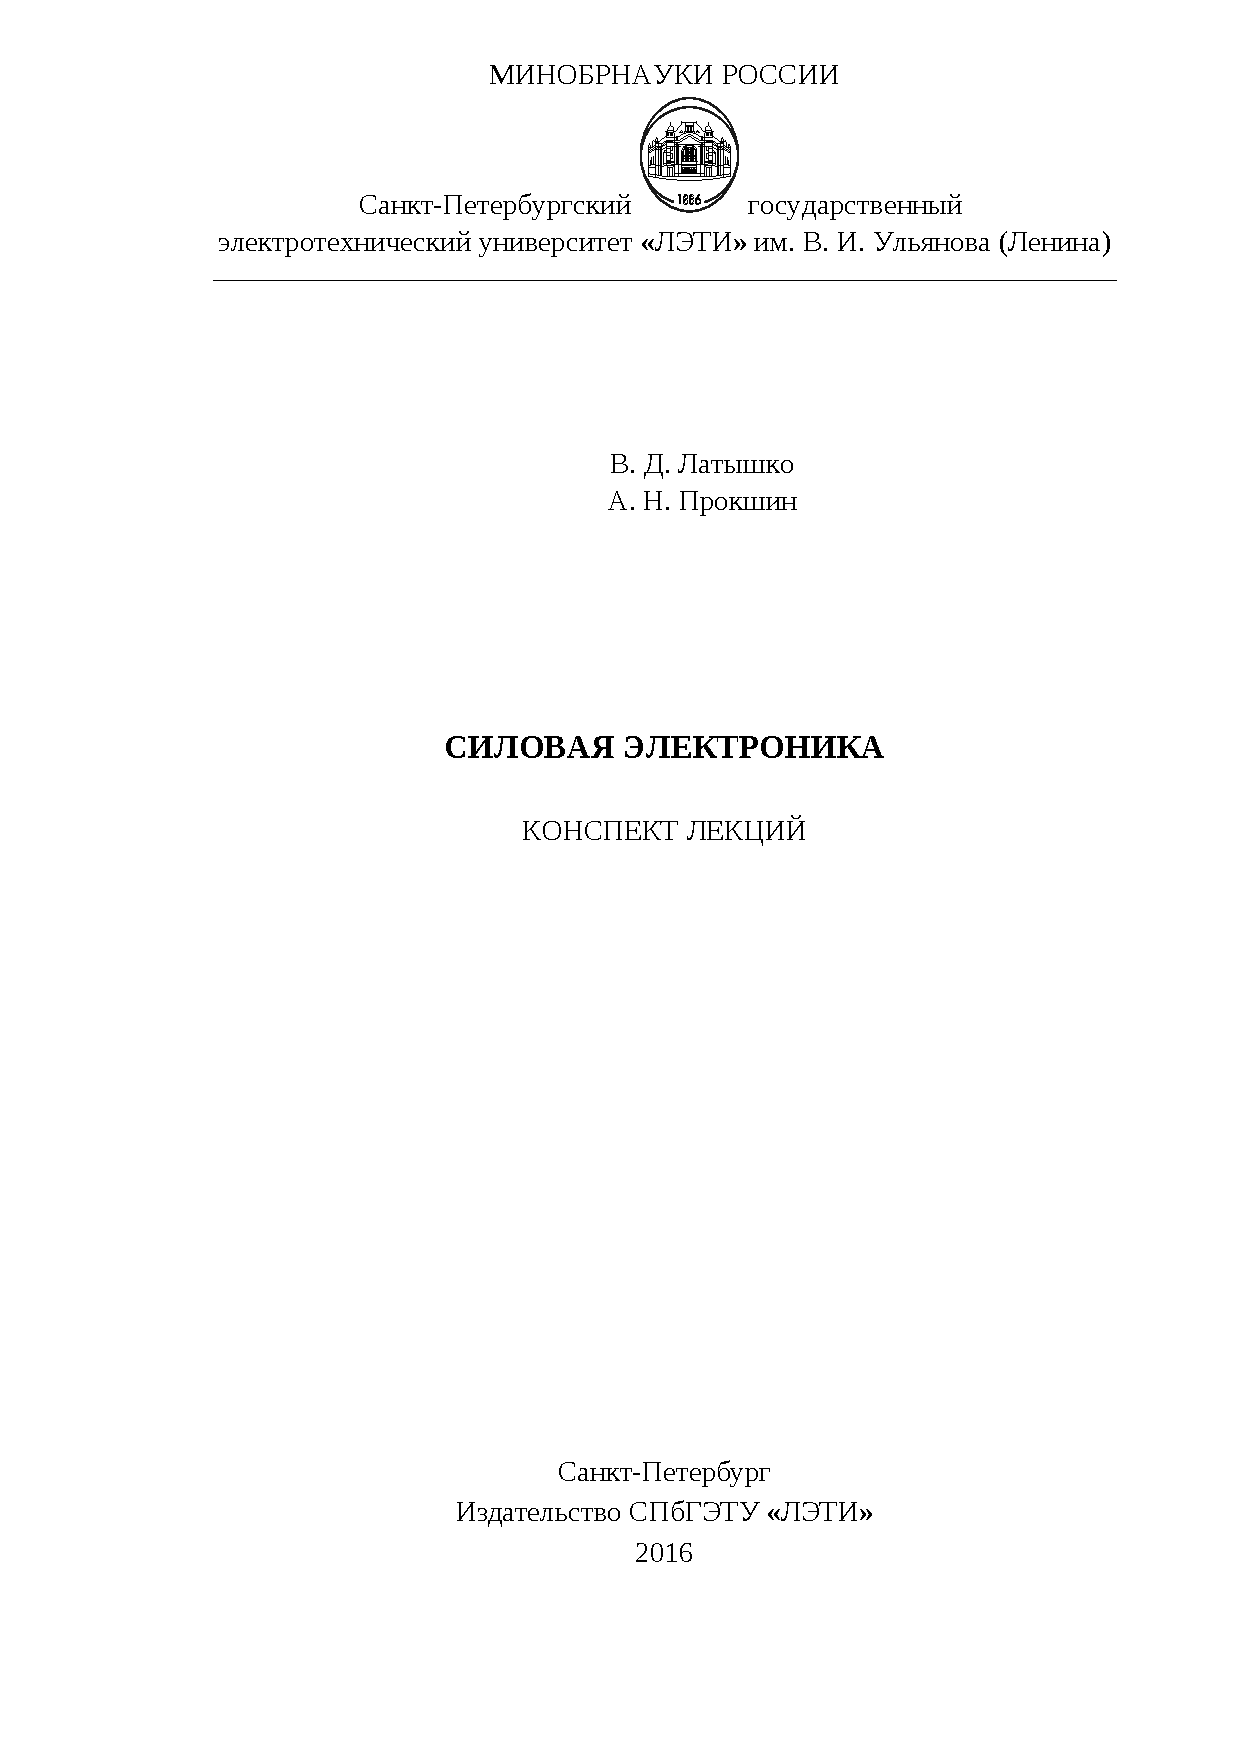
\includepdf[pages=-]{my_1my_12}

\begin{abstract}
	Излагаются принципы преобразования электрической энергии: выпрямления, инвертирования, преобразования частоты и др. Описаны основные схемы преобразовательных устройств, способы управления ими и регулирования основных параметров, показаны области рационального использования различных типов преобразователей.

	Конспект лекций по дисциплине «Силовая электроника» предназначен для бакалавров по направлению подготовки 13.03.02 «Электроэнергетика и электротехника» профилю «Электропривод и автоматика».

\end{abstract}


\tableofcontents
\newpage

Дисциплина называется Силовая Электроника. Также есть синонимы
Силовая Преобразовательная техника, Энергетическая электроника.

Кафедра РАПС -- первая в стране кафедра электропривода.
Дисциплина начиналась с Промышленной электроники. Электронные приборы и
устройства. Есть наука о приборах и устройствах, нелинейных.

Промышленная электроника -- это продолжение ТОЭ в область нелинейных
устройств.
Может быть недостаточно для современного специалиста. Может оказаться
недостаточно

\begin{tabular}{c}
  приборы\\
  электрические цепи\\
  электронные устройства\\
  управление, хранение, обработка информации
\end{tabular}

Было 200 часов, на силовую электронику 280 часов. Сейчас даже курсового
проекта нет. Методички по курсовому проекту будут полезны для расчетов.

Дисциплина относится к силовым устройствам
\begin{itemize}
\item Генераторы Г
\item Двигатели М
\item Трансформаторы Т
\item UZ -- преобразователи электрической энергии из одного вида в другой.
\end{itemize}

Какие параметры электрической энергии известны?:
\begin{itemize}
\item $U_{mo}$ в розетке
\item $U$
\item $f$
\item число фаз
\item ``Форма''  
\end{itemize}  
  
$G$ преобразует механическую энергию в электрическую.
Аккумулятор не зарядишь переменным током. Электролиз -- аллюминий из бокситов,
требует постоянного тока.
Управление скоростью двигателей в производстве.

Чего в мире больше: $G$, $M$, $T$, $UZ$?
Лифт не круглосуточный, предприятия ночью не работают. $G$ не загружены
полностью. $T$ -- по мощности больше всего. В среднем от одного $G$ до
потребителя 3.5 $T$ трансформатора. 6,10,35kV.

Электропривод, управляющий механизм. Электролиз, гальваника.

Задан вопрос на который у самого нет ответа.

\begin{tikzpicture}
  \draw (2,0) rectangle (5,2);
  \draw[->] (0,1)--(1.8,1) node[midway, above] {$U^\prime, f^\prime$}
  node[midway, below] {$m^\prime,(\phi^\prime)$};
  \draw[->] (5,1)--(7,1) node[midway, above] {$U^{\prime\prime}, f^{\prime\prime}$}
  node[midway, below] {$m^{\prime\prime},(\phi^{\prime\prime})$};
  \draw[<-] (3.5,-0.1) -- (3.5,-0.4) node[below]{$U_\textcyrillic{упр}$};
  \draw[<-,thin] (4,-0.6) -- (4.5,-0.6) node[right]{информационный вход};
  \draw (3.5,2)node[above] {$UZ$};  
  \draw[<-,thin] (6.7,1.3)--(7.5,1.5) node[right]
       {\begin{tabular}{l}вот этим хочу\\управлять, если не\\нужно, то нерегулируемый\end{tabular}};
\end{tikzpicture}

\section{Силовые полупроводниковые приборы}
Нарисую УГО прибора:

\begin{circuitikz}
  \draw
  (0,0) node[nfet] (nfet) {}
  (nfet.drain) node[anchor=south] {сток}
  (nfet.source) node[anchor=north] {исток}
  (nfet.gate) node[anchor=east] {затвор}
  (nfet.base) node[anchor=west] {подложка}
  (2,0) node[right] {\begin{tabular}{l}транзистор полевой\\
      с изолированным каналом\\
      канал встроенный\\
  чаще контакты соединяют\end{tabular}}
  (8,0) node[nigfete] (nigfete) {};
\end{circuitikz}

\begin{circuitikz}
  \draw
  (1,0) node[nigbt] (nigbt) {}
  (3,0) node[right] {IGBT с индуцированным затвором}
  ;\end{circuitikz}


Я знаю, что читали приборы. Приборы надо знать, надо знать их характеристики,
как ими пользоваться.

Чем силовые полупроводниковые приборы отличаются от несиловых: мощность,
габариты.

\begin{circuitikz}
  \draw
  (0,1) to[Ty,n=ty1] (0,0)
  (ty1.gate) node[anchor=east] {|} node [anchor=west] {управляющий электрод}
  (0,-0.5) node[right] {запираемый тиристор}
  ;\end{circuitikz}

\begin{tikzpicture}
  \draw (0,0)rectangle(0.5,0.5)
  (0,0.5)rectangle(0.5,1)
  (0,1)rectangle(0.5,1.5)
  (0,1.5)rectangle(0.5,2)
  (0.25,0.25) node {n}
  (0.25,0.75) node {p}
  (0.25,1.25) node {n}
  (0.25,1.75) node {p}
  (0.25,-0.5)--(0.25,0) node[midway,below right] {Катод}
  (0.25,2)--(0.25,2.5) node[midway,above right] {Анод}
  (-0.5,0.75)--(0,0.75) node[midway,below left] {управляющий электрод}
  ;\end{tikzpicture}

\begin{tikzpicture}
  \draw
  (0,0) node[nmos] {};
  \draw[<-] (-0.5,0.7) -- (0,1.2) node[above right] {канал типа n};
\end{tikzpicture}  

В течении двух недель изучить по любому учебнику по СПП
(силовые полупроводниковые приборы). По программе ну отведено ни одного
часа.

Силовые полупроводниковые приборы начали применятся с середины XX века.
До этого были ионные приборы, электровакуумные.
Чем они были хуже будем оценивать с точки зрения силовой электроники.
Допустим, что нет никаких приборов, ни ионных, ни электровакуумных на планете.

Были механические преобразователи

\begin{tikzpicture}
  \draw (0,0) circle(0.5)
%  (-0.375,-0.35)--(-0.75,-0.35)--(-0.75,0.35)--(-0.357,0.35)
%  (0.357,-0.35)--(0.75,-0.35)--(0.75,0.35)--(0.357,0.35)
  (0,0) node {M}
  (-1,-1) circle(0.5)
  (-1,-1) node{Г};
  \draw[thick](-0.643,-0.65)--(-0.2,-0.2);
  \draw[->] (-0.5,0)--(-0.75,0)--(-0.75,0.75)--(-0.25,0.75)--(-0.25,1.25);
  \draw[->] (0.5,0)--(0.75,0)--(0.75,0.75)--(0.25,0.75)--(0.25,1.25);
  \draw[->] (-0.8,-1.1) -- ++(0.8,-0.4)
;\end{tikzpicture}

И получу на выходе, что что мне нужно:
$\textcyrillic{Э}\rightarrow \textcyrillic{М} \rightarrow \textcyrillic{Э}$.
У силовых преобразователей КПД самый главный параметр. В компьютере всё
по-другому.

Что такое управляемый прибор?
\begin{circuitikz}\draw
  (0,1)to[Do,v^=$ $](0,0)
  ;\end{circuitikz}

\begin{circuitikz}\draw
  (0,0)node[nmos](nmos) {}
  [thin](nmos.gate) -- ++ (-0.8,0)
  (-2,-0.6) -- (0,-0.6) node[at start, above] {управление}
;\end{circuitikz}

Сопротивление меняется, можно плавно регулировать, значит $R$ меняется,
значит не могу силовой прибор использовать.

Чем отличается ЭДС от напряжения? В розетке ЭДС или напряжение.
Напряжением будем считать ЭДС + плюс падение на внутреннем сопротивлении.

\begin{circuitikz}
  \draw
  (0,2)to[short,o-](1,2)to[R,l^=$R_\textcyrillic{нагр}$](2,2)
  (2,2)--(2,1.4)
  (2,1)circle(0.4)
  (2,0.6)--(2,0)to[short,-o](0,0)
  (2,1) node {M}
  (0,1) node {E};
  \draw[->] (1.2,1)--(1.55,1);
  \draw(2.5,1) node[right] {\begin{tabular}{l}
      $ER$ -- максимальный ток\\
      если в 2 раза уменьшить\\
      то $R$ возрастет.\\
      Не годится управлять через $R$
  \end{tabular}}
;\end{circuitikz}

{\it Все полупроводниковые приборы должны работать в ключевом режиме --
  железное правило}

Как во всяком правиле есть исключения: если мощность не очень большая.

Неразумно отводить мощность от полупроводникового прибора(ПП), поэтому
используется ключевой режим.

Импульсный режим 0,100,0,100 -- 50\%

\begin{tikzpicture}\draw
  (0,0)--(0.25,0)--(0.25,1)--(0.5,1)--(0.5,0)--(0.75,0)--(0.75,1)--(1,1)
  --(1,0)--(1.25,0)--(1.25,1)--(1.5,1)--(1.5,0)--(1.75,0)
  (0,-0.5) node[right] {500 Герц}
;\end{tikzpicture}

Таким фильтром обычно является сама нагрузка. Если этого не хватает,
то добавим фильтр.

\section{Классификация силовых полупроводниковых преобразователей
  электрической энергии}

Существует много классификаций, в основу кладется тот иил иной
классификационный признак. Мы сделаем классификацию на основе противопоставления
переменного и постоянного тока. Выпрямитель напряжения или тока?
Немного нефизично. $I$ -- производить основную работу(ампер-часы).
Но $U$ является средством получения тока. Так что можно говорить и то и другое.

\hspace{-3cm}
\begin{tikzpicture}\draw
  (0,10.3)rectangle(16.2,11.1)
  (8,10.7) node {\large Преобразователь Параметров Электрической Энергии}
  (1.9, 9.4) node {\large выпрямитель}
  (0,8.4)rectangle(3.8,9.2);
  \draw[->] (1.5,7.6) -- (0.8,6.8);
  \draw[->] (1.9,7.6) -- (2.6,6.8);
  \draw(1.9, 8.8) node {\larger[3] $\sim$ $\rightarrow$ $=$}
  (5.9, 9.4) node {\large инвертор}
  (4,8.4)rectangle(7.8,9.2)
  (5.9, 8.8) node {\larger[3] $=$ $\rightarrow$ $\sim$}
  (8,8.4)rectangle(12.2,9.2)
  (9.9,9.7) node{\larger[1] \begin{tabular}{c}Преобр. переменного\\
      напряжения\end{tabular}}
  (9.9, 8.8) node {\larger[3] $\sim$ $\rightarrow$ $\sim$}
  (14.3,9.7) node{\larger[1] \begin{tabular}{c}Преобр. импульсов\\
  постоянного напряжения\end{tabular}}
  (12.4, 8.4)rectangle(16.2,9.2)
  (14.1, 8.8) node {\larger[3] $=$ $\rightarrow$ $=$}
  (4,8) node {\begin{tabular}{c}может быть импульсное управление\\
      может быть фазное. фазное--удобнее\end{tabular}}
  (10,8) node{\begin{tabular}{c}могут быть\\фазные методы\end{tabular}}
  (14.3,7.8) node{\begin{tabular}{c}широтно-импульсная\\
      фазово-импульсный\\частотно-импульсная\end{tabular}}

  (3,7.15) node[right] {\begin{tabular}{c}в сеть,на 
      гото-\\вую синусоиду\end{tabular}};
  \draw[thin,->] (4.6,7.4)--(5,8.35);
  \draw
  (4,5.7)rectangle(6,6.7)
  (5,6.2) node{\begin{tabular}{c}Зависимый\\инвертор\end{tabular}} 
  (4.8,4.4) node{\begin{tabular}{c}солнечная\\батарея\\
      в розетке 50Гц\\я должен дать 50\\
      по форме,частоте,\\амплитуде\end{tabular}}  
  (6.2,5.7)rectangle(8.5,6.7)
  (7.3,6.2) node{\begin{tabular}{c}Автономный\\инвертор\end{tabular}}
  (7.3,5.2) node{\begin{tabular}{c}паяльник\\я сам хозяин\end{tabular}};
  \draw[->] (7.1,4.8) -- (6.1, 3.1);
  \draw[->] (7.3,4.8) -- (7.3, 3.1);
  \draw[->] (7.5,4.8) -- (8.5, 3.1);
  \draw (5.6,2.2)rectangle(6.6,3.0)
  (6.1,2.6) node {АИН}
  (6.8,2.2)rectangle(7.8,3.0)
  (7.3,2.6) node {АИТ}
  (8,2.2)rectangle(9,3)
  (8.5,2.6) node {АИР}
  (-1.2,5.7)rectangle(1.4,6.7)
  (0.1,6.2) node{\begin{tabular}{c}неуправляемый\\выпрямитель\end{tabular}}
  (1.6,5.7)rectangle(3.8,6.7)
  (0.1,5.0) node{\begin{tabular}{c}диод,управля-\\емый силовой\\
      цепью\end{tabular}}
  (2.7,6.2) node{\begin{tabular}{c}управляемый\\выпрямитель\end{tabular}};
  \draw[->] (2.5,5.6)--(0.2,3.1);
  \draw[->] (2.7,5.6)--(2.6,3.1);
  \draw(-1.2,2.2)rectangle(1.2,3.0)  
  (0,2.6) node {нереверсивные}
  (1.4,2.2)rectangle(3.8,3.0)
  (2.6,2.6) node {реверсивные}
  (2.6,1.4) node {\begin{tabular}{c}2 тиристора\\в обоих\\напралениях
  \end{tabular}}
  ;  
  \draw[->](6.1,7.5)--(5.7,6.75);
  \draw[->](6.3,7.5)--(7.3,6.75);

  \draw (10.4,6.2) node {\begin{tabular}{c}частоту,число фаз\\
      если только\\уровень, то\\
      регулятор переменного\\
      напряжения
  \end{tabular}}
  (9.0,3.7)rectangle(10.0,4.5)
  (9.5,4.1) node {РПН}
  (10.8,3.7)rectangle(11.8,4.5)
  (11.3,4.1) node {НПЧ}
  (11.2,2.8) node {\begin{tabular}{c}непосредст-\\венный\\преобразова-\\
      тель частоты\end{tabular}};
  \draw[->] (10.2,5.2)--(9.5,4.6);
  \draw[->] (10.6,5.2)--(11.3,4.6);
  \draw (14.2,6.2) node {\begin{tabular}{c}только уровень\\
      частота ``0''\\формы нет\end{tabular}}
  (12.4,4)rectangle(13.8,4.8)
  (13.1,4.4) node{\begin{tabular}{c}ревер-\\сивный\end{tabular}}
  (14,4)rectangle(15.8,4.8)
  (14.9,4.4) node{\begin{tabular}{c}неревер-\\сивный\end{tabular}};
  \draw[->](14,5.6)--(13.1,4.9);
  \draw[->] (14.4,5.6)--(14.9,4.9)
;\end{tikzpicture}

АИН --формирует на выходе кривую напряжения.
АИТ -- формирует на выходе кривую тока.
Помним, что все приборы работают в ключевом режиме.

\begin{circuitikz}\draw
  (0,0)--(1.5,0)to[short,-o](1.5,0.75)to[short,o-*](1.5,1.5)
  to[short,*-o](1.5,2.25)--(1.5,3)--(0,3)--(3,3)
  to[short,-o](3,2.25)to[short,o-*](3,1.5)to[short,*-o](3,0.75)
  to[short,o-](3,0)--(1.5,0)
  (0,3) node[left] {{\large +}}
  (0,0) node[left] {{\large --}}
  (1.5,1.5)to[european resistor](3,1.5)
  (1.5,2.25) node[above left] {1}
  (1.5,0.75) node[below left] {2}
  (3,2.25) node[above right] {3}
  (3,0.75) node[below right] {4};
  \draw[->] (1,2.25)--(1.35,2.25);
  \draw[->] (1,0.75)--(1.35,0.75);
  \draw[->] (2.5,2.25)--(2.85,2.25);
  \draw[->] (2.5,0.75)--(2.85,0.75);
  \draw[<-] (3.45,2.4)--(4,3) node[right]{заменяем рубильниками};
  \draw (4.5,2.5)--(5.5,2.5)--(5.5,1.8)
  to[european resistor](7,1.8)--(7,1)--(8,1);
  \draw[<-] (6.5,2.1)--(7.5,2.3) node[right]
       {ток течет слева направо};
  \draw (4.5,-1.2)--(5.5,-1.2)--(5.5,-0.4)
  to[european resistor](7,-0.4)--(7,0.4)--(8,0.4);
  \draw (-2,1)--(-1,1)
  (-2,-1)--(-1,-1)
  (-1.5,-1)to[C,*-*](-1.5,1)
  (-1.5,1.2) node[above] {включаем};
  ;\end{circuitikz}

\begin{tikzpicture}
  \draw[thin,->] (0,0)--(5,0) node[right,below] {t};
  \draw[thin,->] (0,-1.2)--(0,1.3) node[left] {$I$};
  \draw[thin,->] (0,3)--(5,3) node[right,below] {t};
  \draw[thin,->] (0,1.8)--(0,4.3) node[left] {$U$};
  \draw (0,0)--(0.5,1)--(1.5,-1)--(2.5,1)--(3.5,-1)--(4.5,1)
  (0,4)--(0.5,4)--(0.5,2)--(1.5,2)--(1.5,4)--(2.5,4)--(2.5,2)--
  (3.5,2)--(3.5,4)--(4.5,4)--(4.5,2);
  \draw[<-] (5,3.5)--(6,3.5) node[right] {Это напряжение};
  \draw[<-] (5,2.2)--(6,1.8) node[right]
       {\begin{tabular}{c}а также ток\\при активном сопротивлении
       \end{tabular}};
       \draw[<-] (5,-0.5)--(6,-1) node[right] {индуктивное};
 \draw (-0.8,0) node[left] {${\displaystyle L\frac{di}{dt}=U}$}
 ;\end{tikzpicture}

Конденсатор ставить в качестве нагрузки нельзя

${\displaystyle i_c = C\frac{du_c}{dt}}\;\;\;$
${\displaystyle \frac{du}{dt}=\infty}$

Если нельзя, но очень хочется то можно

\begin{tikzpicture}\draw
  (0,0)--(2.5,0)--(2.5,0.75)to[short,o-o](2.5,2.25)--(2.5,3)
  (0,3)--(1,3)to[L](2.5,3)
  (1,0)to[C,*-*](1,3)
  (2.5,1.5)to[european resistor,*-](3.5,1.5)to[C](4.5,1.5)to[L,-*](5.5,1.5)
  (2.5,0)--(5.5,0)--(5.5,0.75)to[short,o-o](5.5,2.25)--(5.5,3)--(2.5,3);
  \draw[<-] (1.85,3.3)--(3,3.6) node[right] {добавим};
  ;\end{tikzpicture}

Включаем в нагрузку. Ток в этой индуктивности

\begin{tikzpicture}
  \draw[thin,->](0,-1)--(0,1.3) node[left] {$I$};
  \draw[thin,->] (0,0)--(5,0) node[right, below] {$t$}; 
  \draw(0,1)--(0.5,1)--(0.5,-1)--(1.5,-1)--(1.5,1)--(2.5,1)--(2.5,-1)--
  (3.5,-1)--(3.5,1)--(4.5,1)--(4.5,-1);  
\end{tikzpicture}

Если вставили индуктивность на входе, то теперь индуктивность в нагрузку нельзя.
Если на входе индуктивность, то индуктивность в нагрузку нельзя.


\begin{circuitikz}\draw
  (0,3)to[L](1.5,3)--(1.5,2.25)to[short,o-o](1.5,0.75)--(1.5,0)--(0,0)
  (1.5,1.5)--(2,1.5)to[L](3,1.5)to[R](4,1.5)--(4.5,1.5)
  (2,1.5)--(2,2.25)to[C](4,2.25)--(4,1.5)
  (1.5,0)--(4.5,0)--(4.5,0.75)to[short,o-o](4.5,2.25)--(4.5,3)--(1.5,3)
;\end{circuitikz}  

АИР(автономный инвертор резонансный) резонансного типа.
Для нашей специальности не очень подходит. Резонансный -- значит
частоту изменить не можем.
Применяется для закалки стали.

Сокращаем количество до 8ми. Генераторы $\rightarrow$ Моторы.

\begin{tikzpicture}\draw
  (0,2)rectangle(2.5,2.8)
  (1.25,2.4) node {{\larger[2] $\sim$ $\rightarrow$ $=$}}
  (3,2)rectangle(5.5,2.8)
  (4.25,2.4) node {{\larger[2] $=$ $\rightarrow$ $\sim$}}
  (2.75,0.5)ellipse(2.7cm and 0.7cm)
  (1.8,0.5) node {\begin{tabular}{c}управляемый\\выпрямитель\end{tabular}}
  (4.1,0.5) node {\begin{tabular}{c}зависимый\\инвертор\end{tabular}};
  \draw[->](1.25,2)--++(0.75,-0.75);
  \draw[->](4.25,2)--++(-0.75,-0.75);
  ;\end{tikzpicture}

Если энергия пошла в обратную сторону. Рассмотрим управляемый выпрямитель.

НПР $\leftrightarrow$ Реверсивный выпрямитель. При одном направлении тока,
а если поставить второй транзистор. И ток и напряжение можно инвертировать.

Переменное напряжение $\sim$ -- это постоянное, которое меняется по
уровню и направлению.

$50 \sim = \sim 500$

Непосредственный -- это не 2х ступенчатый преобразователь
(преобразователь частоты со звеном постоянного тока).

Это классификация одноступенчатых преобразователей.

НПЧ -- одноступенчатый преобразователь!

Реверсивный постоянного $\leftrightarrow$ АИН. Осталось 8, но это неполная
классификация.

\begin{tikzpicture}
  \draw (0,-0.25)rectangle(2.5,0.25)
  (1.25,0) node {\larger[2] $=$ $\rightarrow$ $=$};
\end{tikzpicture}
-- по квадрантам.

Другие классификационные признаки, выбирается параметр, по нему
идет классификация.

2-й параметр) по типам силовых полупроводниковых приборов.

\begin{tabular}{lcl}
  неуправляемые &--&диоды \\
  управляемые &--& однозначно тиристоры
\end{tabular}

Транзисторов достаточно много. Тиристор -- отпираемые, незапираемые по
управляющему току семистор.

3-й параметр) -- тип силовой схемы.

\begin{tabular}{lcl}
нулевые схемы &--& трансформаторы с выводом ``0''-й точки.\\
мостовые& -- &содержат две нулевых.(Одна схема -- объединены катоды,\\
&&другая -- аноды)\\
кольцевые&&\\
комбинированные&&
\end{tabular}

\begin{circuitikz}\draw
  (0,2.7)--(2,2.7) node[right] {``0''} 
  (0,2) node[above] {A} to[D*](0,1)--(2,1)
  (1,2) node[above] {B} to[D*](1,1)to[short,-*](1,0.5)
  (2,2) node[above] {C} to[D*](2,1);
  \draw[<-] (1.2,0.5) -- (2.5,0.5) node[right]
  {так не говорят, что эта точка ``0''-я}
  ;\end{circuitikz}


\begin{circuitikz}\draw
  (3,0)to[D*](2,0)--(1,0)to[D*](0,0)
  (3,0.75)to[D*](2,0.75)--(1,0.75)to[D*](0,0.75)
  (3,1.5)to[D*](2,1.5)--(1,1.5)to[D*](0,1.5)
  (0,0)--(0,1.5)
  (3,0)--(3,1.5)
  (1,1.5)--(1,2) node[above] {A}
  (1.5,0.75)--(1.5,2) node[above] {B}
  (2,0)--(2,2) node[above] {C}
  (3.8, 0.75) node[right] {мостовая}
  ;\end{circuitikz}  

\begin{circuitikz}\draw
  (1,0)to[D*](2,0)
  (1,0)to[D*](0.29,0.71)
  (1,1.42)to[D*](0.29,0.71)
  (1,1.42)to[D*](2,1.42)
  (2.71,0.71)to[D*](2,1.42)
  (2.71,0.71)to[D*](2,0)
  (1,1.42)--(1,2)--(3,2)
  (2,1.42)--(2,2.4)--(0,2.4)
  (0.29,0.71)--(-.3,0.71)
  (2.71,0.71)--(3.3,0.71)
  (1,0)--(1,-0.6)--(3,-0.6)
  (2,0)--(2,-1)--(0,-1)
  ;\end{circuitikz}

4-й признак

С трансформатором или нет. Трансформатор может быть на входе и на выходе.

\begin{circuitikz}\draw
  (0,0)rectangle(2.4,0.6)
  (1.2,0.3) node {Выпрямитель}
  (1.2,0.6) node[above] {на входе}
  (3,0)rectangle(4.8,0.6)
  (3.9,0.3) node {Инвертор}
  (3.9,0.6) node[above] {на выходе}
  ;\end{circuitikz}

5-й признак -- число фаз

6-й признак -- по уровню напряжения >1000Вольт
В последних гостах по среднему уровню напряжения $6|10|35$ kV.

7-й признак -- по назначению.

\begin{tabular}{l}
для возбуждения\\
для зарядки (электрокары)\\
для гальваники
\end{tabular}

8-й признак -- по конструктивному обозначению

\begin{tabular}{lll}
  IR &--& защитная оболочка от окружающей среды\\
  &IR=0& открытое \\
  &IR=23&\\
  &IR=65& пыле-влаго
\end{tabular}

Классификация, на нее буду ссылаться

По приборам или перейти к первому типу.

\begin{tabular}{l}
  Диоды\\
  \hline\\
  обычные\\
  быстровосста-\\навливающиеся\\
  Шотки
\end{tabular}
\begin{tabular}{l}
  Тиристоры\\
  \hline\\
  обычные\\
  симметричные(симисторы)\\
  запираемые\\
\end{tabular}
\begin{tabular}{l}
  Транзисторы\\
  \hline\\
  биполярные\\
  униполярные\\
  pn переходом\\
  с изолированным затвором\\
  со встроенным\\
  с индуцированным
\end{tabular}

Варисторы, стабилитроны(кремнивые ограничители). Везде делается акцент
на большую мощность.

9-й признак -- диапазон мощности современных устройств от зарядки
телефона, до линий передач постоянным током $10^4$, была линия $10^5$ Вольт.

\begin{tabular}{ll}
  $U$& $10^0$..$10^4$В\\
  $I$& $10^{-2}$..$10^4$А\\
  $P$& $10^{-1}$..$10^6$-$10^7$Вт\\
  $T$& 0;0..50,100,200,400Гц..$10^4$ ($10^5$Hz)
\end{tabular}

$10^5$ используется несущая частота, а не рабочая частота.
--- доли микрогенри, 1MGz -- это сопротивление значительное.

\section{Выпрямители}
Установки большой мощности всегда трехфазные. В квартирах разводятся так,
чтобы напряжение было приблизительно одинаковые в среднем для разных фаз.
Будем использовать однолинейное изображение многофазных сетей

\begin{circuitikz}\draw
  (0,1.5)--(0,1)to[C](0,0)
  (-0.3,0)--(0.3,0)
  (-0.1,0.9)--(0.1,1.1)
  (-0.1,1)--(0.1,1.2)
  (-0.1,1.1)--(0.1,1.3)
  (1,0.75) node {{\larger[3] =}}
  (2,1.5)to[C](2,0.5)
  (2.75,1.5)to[C](2.75,0.5)
  (3.5,1.5)to[C](3.5,0.5)
  (2,0.5)--(3.5,0.5)
  (2.75,0.5)--(2.75,0)
  (2.45,0)--(3.05,0)
  (6,1.5)--(6,1)to[C](6,0)
  (5.9,1)--(6.1,1.2) node[right] {12}
  (5.7,0)--(6.3,0)
  ;\end{circuitikz}

\begin{tabular}{cl}
  $U$ & $u=f(t)$\\
  $E$ & e\\
  $I$ & i
\end{tabular}

$I$ -- действующее или среднеквадратичное значение. Постоянное по направлению и есть
пульсации.

\begin{tikzpicture}
  \draw[thin,->] (0,0)--(0,2.3);
  \draw[thin,->] (0,0)--(4,0);
  \draw[domain=0.1:4.7,smooth]
  plot(\x,{1.6 + 0.1*sin((10*\x) r)});
  \draw[<->] (1,0.1)--(1,1.45) node[midway,left] {$I_d$};
  \draw[<->] (2.2,0.1)--(2.2,1.45) node[midway,right] {$i_d$};
  \draw[<-] (2.8,0.8)--(4.2,1.2) node[right] {direct -- прямое, выпрямленное};
  \draw(4.2,0.7) node[right] {для постоянного тока большая буква $I_d$}
;\end{tikzpicture}

\begin{circuitikz}\draw
  (0,0)rectangle(1.5,1)
  (0.75,0.5) node {F}
  (0,1.8)rectangle(1.5,2.6)
  (1.25,2.2)to[Ty](0.25,2.2)
  (0.75,2.6)--(0.75,3.15)
  (0.2,1)--(0.2,1.8) node[midway,left] {{\larger[2] +}}
  (1.3,1)--(1.3,1.8) node[midway,right]{{\larger[2] --}}
  (0.75,3.6) circle(0.45)
  (0.75,4.05) circle(0.45)
  (0.75,4.5)--(0.75,5.3)--(0.25,5.8)
  (0.65,5.4)--(0.55,5.3)--(0.35,5.5)--(0.45,5.6) %выключатель
  (0.75,5.6) node[right] {$QF_1$ -- переменного тока}
  (0.65,4.7)--(0.85,4.9)
  (0.65,4.8)--(0.85,5)
  (0.65,4.9)--(0.85,5.1)
  (0.75,5.8)--(0.75,6.3)
  (-0.4,6.3)--(1.5,6.3)
  (-0.1,6.2)--(0.1,6.4)
  (0,6.2)--(0.2,6.4)
  (0.1,6.2)--(0.3,6.4)

  (1.5,0.8)--(2.5,0.8)--(3,1.3)
  (3.1,0.9) node[above right] {$QF_2$ -- постоянного тока}
  (2.6,0.9)--(2.5,1.0)--(2.7,1.2)--(2.8,1.1) % выключатель
  (3,0.8)--(4.5,0.8)to[european resistor, bipoles/length=1.5cm](6.3,0.8)
  (1.5,0.2)--(6.3,0.2) --(6.3,0.8)
  (1.5,0.2) node[below right] {\larger[2] +}
  (1.5,0.8) node[above right] {\larger[2] --}

  (8,5) to[ospst,l_={S -- switch}] (8,6)
  (7.3,4.2) node[right] {QF -- в силовых цепях}
  (7.5,3.5)to[european resistor](8.5,3.5) node[right] {R}
  (7.5,2.8)--(8,2.8)--(8,3.05)arc(90:360:0.25)--(8.5,2.8) node[right] {L}
  (7.5,2.1)to[C](8.5,2.1) node[right] {C}
  (7.5,1.4)to[battery1](8.5,1.4) node[right] {B}
  (7.5,0.7)to[fuse](8.5,0.7) node[right] {F}

  (-1.7,1.6)rectangle(-0.2,3)
  (-0.95,2.3) node {СУВ}
  ;\end{circuitikz}  

\begin{circuitikz}\draw
  (0,0) node[right] {${\displaystyle C= \varepsilon\frac{S}{d}}$};
  \draw[<-] (1.6,0.3)--(2.4,0.5) node[right] {большое};
  \draw[<-] (1.6,-0.2)--(2.4,-0.2) node[right]
       {\begin{tabular}{c}малое\\пленка\end{tabular}};
  ;\end{circuitikz}  

Электролитический конденсатор пропитан проводящим растворомю создается пленка.
Выключатели по включению по часовой стрелке.
Трансформаторы рисуют так:

\begin{circuitikz}\draw
  (0,1)to[L](0,0)
  (0.75,1)to[L](0.75,0)
  (1.5,1)to[L](1.5,0)
  (0,1)--(1.5,1)
  (0,1.5)--(1.5,1.5)
  (0,1.24)rectangle(1.5,1.26)
  (0,2.5)to[L](0,1.5)
  (0.75,2.5)to[L](0.75,1.5)
  (1.5,2.5)to[L](1.5,1.5)
  ;\end{circuitikz}

VB -- выпрямительный блок. На выходе выпрямителя есть фильтр.

СУВ -- система управления выпрямителя, включает в себя диагностику, измерения,
сигнализацию, контроль, защиты.

Назначение трансформатора:
\begin{itemize}
\item T -- изменяет уровни напряжения
  $$
  U_1 \rightarrow U_2
  $$
\item T -- преобразование числа фаз.
  $$
  m_2 \rightarrow m_1
  $$
\item гальваническая развязка
\item сопротивление К.З.; ограничение тока короткого замыкания Т.К.З. Электрические
  аппараты должны быть устойчивы к токам К.З. Чтобы К.З. не развивалось. Не должно
  приводить к выводу других приборов.

  Есть термическое, динамическое, всё это $I^2_\textcyrillic{КЗ}$.

  $I_\textcyrillic{КЗ}=100$, нагрев $10^4$

  Специальные токоограничивающие реакторы.

  $I_\textcyrillic{КЗ}\approx$ кратен $I_\textcyrillic{ном}$ $5..10..15$ раз.

  Рассмотрим производственное помещение, превышение  $5..10..15$ раз в трансформаторе,
  а для станков это много.
\end{itemize}

T, вернее его $R$ -- естественный ограничитель, в некоторых случаях можно выбросить.
Если нужен только токоограничитель, то ставим токоограничивающий реактор.

\begin{circuitikz}\draw
  (0,0)--(0,0.35)arc(270:0:0.35)--(0,0.7)--(0,2)
  (-0.1,1.2)--(0.1,1.4)
  (-0.1,1.3)--(0.1,1.5)
  (-0.1,1.4)--(0.1,1.6)
  ;\end{circuitikz}

СУВ = СИФУ -- система импульсно-фазового управления. Реализуется теми же программными
средствами в микроконтроллере. выходной сигрнал. через усилитель мощности
подается сигнал.


Фильтр: Всегда задаю вопрос, что такое

\begin{tabular}{ccc}
  R &--& коэффициэнт пропорциональности ${\displaystyle \frac{U}{I}}$\\
  L & --& коэффицэнт пропорциональности ${\displaystyle \frac{\Psi}{I} =
    \frac{\omega \Phi}{I}}$\\
  C &--&${\displaystyle \frac{q}{U}}$
\end{tabular}

Любая из этих величин философская, физическая.
R -- это потери! В нашем случае КПД на первом месте!
\begin{itemize}
\item L
\item C
\item L--C
\item C--L Г-образная
\item C--L--C Т-образная  
\end{itemize}

Основные характеристики фильтра:
Во сколько раз снижается пульсаций.

\begin{circuitikz}\draw
  (0,2)--(2,2)to[L,l={L}](3,2)--(5,2)to[R,l={$R_\textcyrillic{н}$}](5,0)--(0,0)
  (0,1) node {\begin{tabular}{c}U\\u\end{tabular}}
  (2.5,1) node {$U_c + u^\prime$};
  \draw[<->](4,2)--(4,0) node[midway,left] {$u^{\prime\prime}$}
  ;\end{circuitikz}

Обмотка возбуждения генератора это хорошо?

Коэффициэент сглаживания фильтра
${\displaystyle К= \frac{u^{\prime\prime}}{u^\prime}}$

$$
Z = \sqrt{R^2_\textcyrillic{н} + (\omega L)^2}
$$

Отсюда коэффициент сглаживания фильтра =

$K={\displaystyle \frac{u^\prime}{\frac{u^\prime}{z}R_\textcyrillic{н}}}$ =
${\displaystyle \frac{Z}{R_\textcyrillic{н}}} = \sqrt{1 +(\omega T)^2}
\approx \omega T$, при $\omega T = 4$

C-фильтр

\begin{circuitikz}\draw
  (0,2)--(2,2)
  (0,0)--(2,0)
  (1,0)to[C](1,2)
   ;\end{circuitikz}

Пульсация до установки на пульсацию после.
Фильтр будет хорошо действовать когда будут диоды, будет их запирать.

Коэффициэнт сглаживания фильтров -- самостоятельно. Зарисовать схемы.

Это классические реактивные фильтры. Существуют резонансные фильтры.

\begin{circuitikz}\draw
  (0,1.5)--(0.5,1.5)--(0.5,1.15)to[C](1.5,1.15)--(1.5,1.5)
  (0.5,1.5)--(0.5,1.85)to[L](1.5,1.85)--(1.5,1.5)--(2,1.5)
  to[L](2,0.75)to[C](2,0)
  (2,1.5)--(2.75,1.5)to[european resistor](2.75,0)--(0,0);
  \draw[<-] (2.1,0.2)--(3,0) node[right] {для остальных частот добавим} 
  ;\end{circuitikz} Фильтр-пробка  
$$
\omega_\textcyrillic{рез} = \frac{1}{\sqrt{LC}}
$$
Теоретически задержит полностью. Он эффективен только на одной частоте.
$\omega_\textcyrillic{рез}$ -- здесь на резонансной частоте сопротивление 0

В последнее время применяют активные фильтры.

Активный генератор переменной составляющей:

\begin{circuitikz}\draw
  (0,2)to[L](2,2)--(2,1.5)
  (1.5,0.5)rectangle(2.5,1.5)
  (2,1) node {АФ}
  (0,0)--(2,0)--(2,0.5)
  (2,2)--(3.5,2)to[european resistor](3.5,0)--(2,0)
  (1,2.3)node {$i_d$};
  \draw[->](1.3,2.3)--(3.2,2.3);
  \draw[<-] (2.6,1.6)--(3.7,2) node[right]
       {\begin{tabular}{c}в противовазе добавляем\\
           $i^\prime=i^{\prime\prime}$\end{tabular}}
       ;\end{circuitikz}

Это тоже что и резонансный фильтр, но <имеет собственный
источник энергии>. Это тоже преобразователь.

Д.з. -- транзисторы и фильтры.

\section{Элементы защиты}
L и С выдержит пока не горит изоляция.
Основной элемент ПП - кристалл очень малых размеров

Трансформатор,реактор,мотор можно перегружать в десятки раз.
ПП -- граммы. Защита по току очень важна.

ПП -- прочность обратного pn-перехода ограничена. Малое время
для защиты по току(быстродействующая защита).
А по напряжению защит нет. Если перенапряжение состоялось, то всё
распространяется со скоростью света. Защита по напряжению, по недопущению
перенапряжения.

Из-за малой теплоемкости по току защита $10^{-3}...10^{-2}$. Существуют
быстродействующие плавкие предохранителию.

\begin{circuitikz}
  \draw (-0.2,1) node[left] {$I^2 t$ -- Мощность};
  \draw[->](0,0)--(0,2.2) node[left] {$I^2$};
  \draw[->](0,0)--(4,0) node[right] {$t$};
  \draw[domain=0.45:3.5]
  plot(\x, {1/\x});
\end{circuitikz}

Обычные плавкие предохранители олово+медь. Используется плавкая
вставка из технического серебра 99.9\% техническое чистое серебро
(драгоценный, но не благородный метал). Плавкая вставка должна быть
меньше чем ПП, чтобы быстро сгорела -- она должна быть горячей
в нормальном режиме.

$$
W = \left(\int I^2 dt\right)_\textcyrillic{тиристора} >
W_\textcyrillic{предохранителя}
$$
В этом случае тиристор может выдержать.

Все зависит от отношения
$$
\frac{I^2R}{c} \leftarrow \begin{array}{c}\textcyrillic{-- мощность}\\
  \textcyrillic{ -- теплоемкость}
 \end{array}
$$

\begin{circuitikz}
  \draw[->](0,0)--(0,3.2) node[left] {I};
  \draw[->](0,0)--(5.3,0) node[right] {t};
  \draw[domain=0:5]
  plot(\x,{-14*exp(-\x) + 14*exp(-0.6*\x)});
  \draw[domain=0:1]
  plot(\x,3.8*\x);
  \draw (0.7,0)--(0.7,2.2);
  \draw (1.8,0)--(1.8,2.4);
  \draw (3,0)--(3,1.6);
  \draw[<-] (2.2,2.5)--(3,2.8) node[right] {\begin{tabular}{l}
      расплавление\\
      дуга\\
      дуга растягивается
  \end{tabular}};
  \draw[<-] (0.7,-0.1)--(0,-0.4) node[left]
       {\begin{tabular}{l}время\\расплавления\end{tabular}};
  \draw (1.8,-0.4) node[below] {ограничение тока};
  \draw[<-] (3,-0.1)--(3.7,-0.4) node[right] {\begin{tabular}{l}время\\
       отключения\end{tabular}};    
\end{circuitikz}  

\section{Требования ключевого режима}
\begin{circuitikz}\draw
  (0,2)to[short,o-](1,2)--(1.5,2)--(2,2.4)
  (2,2)--(4,2)to[european resistor,l=$Z_\textcyrillic{н}$](4,0)to[short,-o](0,0)
  (1.8,2.4) node[above] {$V_K$}
  (1,2)--(1,2.9)
  (2.6,2)--(2.6,2.9)
  (0,1) node {$U_\textcyrillic{пит}$};
  \draw[->] (0.5,2.7)--(1,2.7);
  \draw[<-] (2.6,2.7)--(3.1,2.7) node[right] {$U_V$};
  \draw[<-] (1.75,1.8)--(1.75,1.3) node[right] {упр};
  \draw[->] (3.2,2.3)--(4,2.3)arc(90:0:0.4)--++(0,-0.1);
  \draw (6.9,1) node {\begin{tabular}{l}волна проводимости\\
      по сечению пробегает\\не мгновенно\end{tabular}}
  (11,1) node {\begin{tabular}{l}$V_D$\\$V_S$\\$V_T$\\
      $V_\textcyrillic{К}$ -- ключ по ГОСТ\end{tabular}}
;\end{circuitikz}  

\begin{circuitikz}
  \draw[->] (0,0)--(0,3.5) node[left] {};
  \draw[thin] (0,0)--(2.5,0) (3.5,0)--(6.5,0) (7,0)--(8.5,0);
  \draw[domain=0:2.5]
  plot (\x, {2.5*exp(-8*(\x-1)*(\x-1)*(\x-1)*(\x-1) -2*(\x-1)*(\x-1))+0.3});
  \draw[domain=3.5:6.5]
  plot (\x, {2.5*exp(-4*(\x-5)*(\x-5)*(\x-5)*(\x-5) -1*(\x-5)*(\x-5))+0.3});
  \draw[thin,snake=snake,segment amplitude = -0.4mm, segment length = 3mm] (2.5,0)--(2.5,2.7);
  \draw[thin,snake=snake,segment amplitude = 0.4mm, segment length = 3mm] (3.5,0)--(3.5,2.7);
  \draw[thin,snake=snake,segment amplitude = -0.4mm, segment length = 3mm] (6.5,0)--(6.5,2.7);
    \draw[thin,snake=snake,segment amplitude = 0.4mm, segment length = 3mm] (7,0)--(7,2.7);
  \draw[thin,loosely dashed] (0.3,3)--(0.3,0) node[below] {$t_1$};
  \draw[thin,loosely dashed] (1.7,3)--(1.7,0) node[below] {$t_2$};
  \draw[thin,<-] (0.3,3)--(0.1,3) node[midway,above] {u};
  \draw[thin] (0.3,3) -- (1.7,3) node[midway,above] {$\delta t_\textcyrillic{вкл}$};
  \draw[thin,<-] (1.7,3) -- (1.9,3);
  \draw[thin,loosely dashed] (4,3)--(4,0) node[below] {$t_3$};
  \draw[thin,loosely dashed] (6,3)--(6,0) node[below] {$t_4$};
  \draw[thin,loosely dashed] (7.3,3)--(7.3,0) node[below] {$t_5$};
  \draw[thin] (0.3,-0.5)--(0.3,-1.5) (6,-0.5)--(6,-1.5);
  \draw[thin,<->] (0.3,-1.3)--(6,-1.3) node[midway,above]
       {$T_K = \frac{1}{f_K}$};
  \draw[thin,<-] (4,3)--(3.8,3) node[midway,above] {};
  \draw[thin] (4,3) -- (6,3) node[midway,above] {$\delta t_\textcyrillic{выкл}$};
  \draw[thin,<-] (6,3) -- (6.2,3);
%  \draw[thin] (0,0)--(0,2.5) 
  \draw (4.2,2.3) node {$\scriptstyle{\Delta}p$};
  \draw [thin, <-] (4.3,2.2) -- (7.3,1) node[right] {\begin{tabular}{c}мгновенная\\
      мощность\end{tabular}};
  \draw (11.6,3) node {\begin{tabular}{c}как правило\\
      $\delta t_\textcyrillic{выкл} > t_\textcyrillic{вкл}$ \end{tabular}};
  \draw (11.6,1) node {\begin{tabular}{l}построим\\
      кривую мощности\\
      это тепло\\
  ${\scriptstyle \Delta}p = i_V U$\end{tabular}}
  ;\end{circuitikz}

Энергия в секунду $=$ мощность.

${\scriptstyle \Delta}P = \frac{w}{T_K}$ -- энергия в сек, мощность.

$=f_K \int\limits_{t_1}^{t_1 + T_K} U_V i_V dt $

где $f_K$ -- энергия потерь на переключении.

\begin{itemize}
\item мощность,выделяемая в открытом состоянии
  \item мощность в закрытом состоянии
\end{itemize}

$ 1) \gg 2) $

Чем больше частота, тем больше потери, но частоту нужно повышать.

\section{Основные типы полупроводниковых приборов}
Приборы неуправляемые -- диоды
\begin{circuitikz}
  \draw
  (0,1)to[D](0,0)
  (0,1)--(0,0)
  ;\end{circuitikz}

стабилитроны
\begin{circuitikz}
  \draw
  (0,0)to[D](0,1)
  (0,1)--(0,0)
  (0.18,0.62)--(0.18,0.5)
  ;\end{circuitikz}

КСОН -- кремниевый стабилизированный ограничитель напряжения.

варисторы
\begin{circuitikz}
  \draw
  (0,0)to[european resistor](1,0)
  (-0.1,-0.3)--(0.2,-0.3)--(0.8,0.3)
  ;\end{circuitikz}

\begin{tikzpicture}\draw
  (0.4,0.4)--(1,0.4)--(1,1.6)--(0.4,1.6)--(0.4,0.4)
  (0.4,1)--(1,1)
  (0.7,0)--(0.7,0.4)
  (0.7,1.6)--(0.7,2)
  (0.7,0.7) node {n}
  (0.7,1.2) node {p}
  (1.4,0.7) circle(0.1) (1.5,0.7) node[right] {+}
  (0,1.3)circle(0.1) (-0.1,1.3) node[left] {--}
  (0,-0) node {--};
  \draw[->] (0,1.1) -- (0,0.6);
  \draw[->] (1.4,0.9) -- (1.4,1.4);
  
;\end{tikzpicture}

$$
\textcyrillic{транзисторы } 
\left\{\begin{tabular}{lcc}
МДП&--&метал-диэлектрик-полупроводник\\
МОП&--&метал-оксид-полупроводник\\
униполярные\\
с изолированным затвором\end{tabular}\right.
$$

\section{Вольт-амперная характеристика}


%\section{Силовые полупроводниковые приборы}
Должны знать на уровне пользователя.

Первым прибором был электровакуумный (кенотрон).

% http://tex.stackexchange.com/questions/66216/draw-arc-in-tikz-when-center-of-circle-is-specified
\begin{tikzpicture}
\draw(0,1)--(0,2)arc(180:0:0.5)--(1,1)arc(0:-180:0.5)

%(0.3,0.5)--(0.3,{1-sqrt(0.5-0.2*0.2)})arc(180:20:0.2)
(0.25,0.3)--(0.25,{1-sqrt(0.5*0.5-0.25*0.25)})arc(180:20:0.25)
(0.15,0.3)--(0.15,{1-sqrt(0.5*0.5-0.35*0.35)})arc(180:30:0.35)
;
\end{tikzpicture}
Катод с помощью термоэлектронной эмиссии испускает электроны.


\chapter{Основные схемы силовых полупроводниковых преобразователей}
\begin{figure}[H]
  \begin{circuitikz}\draw
    (0,5) -- ++ (0.5,0)
    (0,5) to[short] (0,4.83)
    (0,4.5) circle ( 0.33 cm)
    (0,4.5) node {$e_1$}
    (0,4.16)  to[short] (0,4)
    (0,4) to[R,l=$r_\phi$] (0,3)
    (0,3) to[L,l=$L_\phi$] (0,2)
    (0,2)  to[Ty,l=$\!V_1$] (0,1)
    -- ++ (0,-1)
    -- ++ (0.5,0)
    %
    (1.2,5) to[short,-*] ++ (0.5,0)
    to[short,-*] ++ (1.4,0)
    (1.7,5) to[short] ++ (0,-0.17)
    (1.7,4.5) circle ( 0.33 cm)
    (1.7,4.5) node {$e_k$}
    (1.7,4.16)  to[short] ++ (0,-0.16)
    to[R,l=$r_\phi$] ++ (0,-1)
    to[L,l=$L_\phi$] ++ (0,-1)
    to[Ty,l=$\!V_k$] ++ (0,-1)
    to[short,-*] ++ (0,-1)
    -- ++ (0.8,0)
    (1.2,0) to[short] ++ (0.9,0)
    %
    (3.1,5) -- ++ (0.5,0)
    (3.1,5) to[short] ++ (0,-0.17)
    (3.1,4.5) circle ( 0.33 cm)
    (3.1,4.5) node {$e_{k\!+\!1}$}
    (3.1,4.16)  to[short] ++ (0,-0.16)
    to[R,l=$r_\phi$] ++ (0,-1)
    to[L,l=$L_\phi$] ++ (0,-1)
    to[Ty,l=$\!V_{k\,+\,1}$] ++ (0,-1)
    to[short,-*] ++ (0,-1)
    -- ++ (0.5,0)
    (2.5,0) to[short] ++ (0.5,0)
    %
    (5,5) to[short] ++ (0,-0.17)
    (5,4.5) circle ( 0.33 cm)
    (5,4.5) node {$e_{m}$}
    (5,4.16)  to[short] ++ (0,-0.16)
    to[R,l=$r_\phi$] ++ (0,-1)
    to[L,l=$L_\phi$] ++ (0,-1)
    to[Ty,l=$\!V_{m}$] ++ (0,-1)
    -- ++ (0,-1)
    %    -- ++ (0.5,0)
    (4.5,0) to[short,-*] ++ (0.5,0)
    %
    -- ++ (0.5,0)
%   
    (5.5,5) to[short,-*] ++ (-0.5,0)
    -- ++ (-0.5,0)
    ;\end{circuitikz}
\end{figure}

по госту обозначение диода
\begin{circuitikz}\draw
(0,0) to[Do] (1,0)--(0,0)
  ;\end{circuitikz}.

\begin{circuitikz}
  \draw[thin,->](0,0)--(2,0) node[right] {$\omega t$}
  ;\end{circuitikz}

Значения по оси времени откладываются в угловых единицах $\omega t$.
$\displaystyle{\frac{1}{50}\textcyrillic{сек}} $ -- период. $1msec= 18^\circ$

\begin{circuitikz}\begin{scope}[xscale=2,yscale=3]
    \draw[thin,->] (-pi/2,0) -- (pi+pi/2+pi/12,0) node[right] {$\omega t$};
    \draw[thin,->] (0,-1.1) -- (0,1.2) node[left] {U};

    \draw[thin,dotted,help lines,smooth] (-pi/2,1/2) -- (pi+pi/2,1/2);
    \draw[thin,dotted,help lines,smooth] (-pi/2,-1/2) -- (pi+pi/2,-1/2);
    \draw[domain=0:pi/3,thin,dashed,help lines,smooth]
    plot(\x, {1/(pi/3)*\x -1/2+0.02});
    \draw[domain=2*pi/3:3*pi/3,thin,dashed,help lines,smooth]
    plot(\x, {1/(pi/3)*\x -1/2-2+0.02});
    \draw[domain=-pi/3:0,thin,dashed,help lines,smooth]
    plot(\x, {-1/(pi/3)*\x -1/2+0.02});
    \draw[domain=pi/3:2*pi/3,thin,dashed,help lines,smooth]
    plot(\x, {-1/(pi/3)*\x -1/2+2+0.02});
    \draw[domain=3*pi/3:4*pi/3,thin,dashed,help lines,smooth]
    plot(\x, {-1/(pi/3)*\x -1/2+4+0.02});
    
  \draw[yellow,domain=-pi/2:pi+pi/2]
  plot (\x, {cos(\x r)});
  \draw[green,domain=-pi/2:pi+pi/2]
  plot (\x, {cos((\x-2*pi/3) r)});
  \draw[red,domain=-pi/2:pi+pi/2]
  plot (\x, {cos((\x-4*pi/3) r)});

  \draw[thin,<-] (pi/12, {cos(pi/12 r)}) -- (pi/6, 1.1) node[right] {$e_k=\sqrt{2}E$};
\end{scope}\end{circuitikz}

Обмотки трехфазных трансформаторов могут быть включены звездой
\begin{tikzpicture}\begin{scope}[scale=0.5]\draw
    (0,0)--(0,1)
    (0,0)--({cos(120+90)},{sin(120+90)})
    (0,0)--({cos(240+90)},{sin(240+90)})
;\end{scope}\end{tikzpicture}

Все одноименные точки
\begin{circuitikz}\draw
  (0,0) to[L] (0,1) node[below left] {$\scriptstyle{\bullet}$} 
  ;\end{circuitikz}
соеденины или началами или концами в одну точку. Звезда может быть прямой или
обратной.

\begin{tikzpicture}\begin{scope}[scale=0.5]\draw
    (0,2)--++(0,1)
    (0,2)--++({cos(120+90)},{sin(120+90)})
    (0,2)--++({cos(240+90)},{sin(240+90)})

    (0,0)--(0,1)
    (0,0)--({cos(120+90)},{sin(120+90)})
    (0,0)--({cos(240+90)},{sin(240+90)})

    % сердечник
    (-1,1.2) rectangle (1,1.22);
    \draw[thin,<-] (1.2,1.21) -- (2.2,1.21) node[right] {сердечник};
    \draw (2.2,-0.5) node[right] {прямая звезда}
%    ;\end{scope}\end{tikzpicture}

%\begin{tikzpicture}\begin{scope}[scale=0.5]\draw
    (11,2)--++(0,1)
    (11,2)--++({cos(120+90)},{sin(120+90)})
    (11,2)--++({cos(240+90)},{sin(240+90)})

    (11,0.4)--++(0,-1)
    (11,0.4)--++({-cos(120+90)},{-sin(120+90)})
    (11,0.4)--++({-cos(240+90)},{-sin(240+90)})

    % сердечник
    (10,1.2) rectangle (12,1.22);
%    \draw[thin,<-] (1.2,1.21) -- (2.2,1.21) node[right] {сердечник};
    \draw (13.2,-0.5) node[right] {обратная звезда}
    ;\end{scope}\end{tikzpicture}


\begin{figure}[H]
\begin{tikzpicture}\begin{scope}[scale=0.5]\draw
    (0,2)--++(0,1)
    (0,2)--++({cos(120+90)},{sin(120+90)})
    (0,2)--++({cos(240+90)},{sin(240+90)})
    
    (-1,0)--++(0,1)
    (-1,0)--++({cos(120+90)},{sin(120+90)})
    (-1,0)--++({cos(240+90)},{sin(240+90)})

    (1,0.5)--++(0,-1)
    (1,0.5)--++({-cos(120+90)},{-sin(120+90)})
    (1,0.5)--++({cos(-240+90)},{-sin(240+90)})
    % core
    (-1.5,1.2) rectangle (1.8,1.22);
    %
    \draw[thin,<-] (1,2)--(2,2) node[right] {первичная всегда в сети}
    ;\end{scope}\end{tikzpicture}
\end{figure}

\begin{figure}[H]
\begin{tikzpicture}
  \begin{scope}[scale=0.5]\draw
    (0,0)--++(0,1)
    (0,0)--++({cos(120+90)},{sin(120+90)})
    (0,0)--++({cos(240+90)},{sin(240+90)});
    \draw (0,0)--++(1,0);
    \draw[thin,<-] (1.1,0)--(2.1,0) node[right]{звезда с выведенным нулём}
;\end{scope}\end{tikzpicture}    
\end{figure}

Другой способ соединения обмоток -- теругольник. Треугольник тоже бывает прямой
и обратный.

\begin{tikzpicture}
  \draw
  (0,0)to[L](0,1.5)
  (0,0) node[left] {x}
  (0,1.5)node[left] {a}
  (1,0)to[L](1,1.5)
  (1,0) node[left] {y}
  (1,1.5) node[left] {b}
  (2,0)to[L](2,1.5)
  (2,0)node[left] {z}
  (2,1.5) node[left] {c}
  (0,-0.3) node[below] {U}
  (1,-0.3) node[below] {V}
  (2,-0.3) node[below] {W}
  (0,-0.8) node[below] {R}
  (1,-0.8) node[below] {S}
  (2,-0.8) node[below] {T};
  \draw[thin,<-] (2.4,-0.8)-- (3.5,-0.8) node[right] {в новых работах}
;  \end{tikzpicture}

\begin{tikzpicture}
  \draw
  (0,0)to[L](0,1.5) node[above] {A}
  (0,0) node[left] {(X)}
  (1,0)to[L](1,1.5) node[above] {B}
  (1,0) node[left] {(Y)}
  (2,0)to[L](2,1.5)node[above] {C}
  (2,0) node[left] {(Z)}
  (0,0)--(0,-0.25)--(2,-0.25)--(2,0)
  (1,-0.25)--(1,0)
  %
  (0,-0.38)rectangle(2,-0.36)
  %
  (0,-2)to[L](0,-0.75)--(0,-0.5)--++(2.5,0)
  (1,-2)to[L](1,-0.75)--(0.5,-0.75)--(0.5,-2)--(0,-2)
  (2,-2)to[L](2,-0.75)--(1.5,-0.75)--(1.5,-2)--(1,-2)
  (2,-2)--(2.5,-2)--(2.5,-0.5)
  (0,-0.75)node[left] {a}
  (0,-2)node[below left]{x}
  (1,-2)node[below left]{y}
  (2,-2)node[below left]{z}
  ;  \end{tikzpicture}


Рассмотрим изображение звезду как векторную диаграмму.

\begin{tikzpicture}
  \begin{scope}[scale=0.5]\draw
  (0,0)--++(0,1) --++({-cos(90+120)},{-sin(90+120)})
  (0,0)--++({cos(90+120)},{sin(90+120)})--++({-cos(90+240)},{-sin(90+240)})
  (0,0)--++({cos(90+240)},{sin(90+240)})--++(0,-1)
  ;\end{scope}
\end{tikzpicture} -- зигзаг, результирующий будет сдвинут по фазе относительно
фазы A. На рисунке равноплечный зигзаг, бывает неравноплечный зигзаг. Зигзаги
бывают также обратными

\begin{tikzpicture}
  \begin{scope}[scale=0.5]\draw
    (0,0)--++(0,1) --++({-cos(90+240)},{-sin(90+240)})
    (0,0)--++({cos(90+120)},{sin(90+120)})--++(0,-1)
    (0,0)--++({cos(90+240)},{sin(90+240)})--++({-cos(90+120)},{-sin(90+120)})
    ;\end{scope}
\end{tikzpicture}
Сдвиг фазы 30\% -- равноплечный зигзаг, если зигзаг неравноплечный, то сдвиг
фаз может быть от $0^\circ$ до $60^\circ$

Треугольники бывают правые и левые.
\begin{tikzpicture}\begin{scope}[scale=0.5]\draw
  (0,0)--++(0,1)--++({cos(-30)},{sin(-30)})--++({cos(210)},{sin(210)})
  (3,0)--++(0,1)--++({cos(210)},{sin(210)})--++({cos(-30)},{sin(-30)})
  ;\end{scope}
\end{tikzpicture}


Существует соединение обмоток по схеме шестиугольника
\begin{tikzpicture}\begin{scope}[scale=0.9]
%    \path (0,0) node (a0){} --++(0,1)node(a1){};
    \draw[->] (0,0)--++(0,1) coordinate (a1);
    \draw[->] (a1)--++({cos(30)},{sin(30)}) coordinate (a2);
    \draw[->] (a2)--++({cos(-30)},{sin(-30)}) coordinate (a3);
    \draw[->] (a3)--++(0,-1) coordinate (a4);
    \draw[->] (a4)--++({-cos(30)},{-sin(30)}) coordinate (a5);
    \draw[->] (a5)--++({-cos(-30)},{-sin(-30)})
    ;\end{scope}
\end{tikzpicture}

Звезда и треугольник энергетически эквивалентны друг другу. Никакими
силами не определить разницу между
\begin{tikzpicture}
  \begin{scope}[scale=0.5]
    \coordinate (o) (0,0);
    \coordinate (o1) ({2+1/2*cos(90+120)},{1/2*sin(90+120)});
    \draw (o)--++(0,1)
          (o)--++({cos(90+120)},{sin(90+120)})
    (o)--++({cos(90+240)},{sin(90+240)})
    ({2+1/2*cos(90+120)},{1/2*sin(90+120)})
    --++({cos(60)},{sin(60)})--++({cos(-60)},{sin(-60)})--++(-1,0)
    ;      
    \end{scope}
  \end{tikzpicture}

\begin{tikzpicture}
  \begin{scope}[scale=0.5]
    \coordinate (o) (0,0);
    \draw (o)--++(0,1)
    (o)--++({cos(30)},{sin(30)})
    (o)--++({cos(150)},{sin(150)})
    (o)--++({cos(210)},{sin(210)})
    (o)--++(0,-1)
    (o)--++({cos(330)},{sin(330)})
    
    (3,-0.5)--++(0,1)--++({cos(30)},{sin(30)})--++({cos(-30)},{sin(-30)})--++
    (0,-1)--++({-cos(30)},{-sin(30)})--++({-cos(-30)},{-sin(-30)})

    (1.8,0) node {$\Longleftrightarrow$};
     
  \end{scope}
  \end{tikzpicture} -- также никакими силами не определить разницу

\begin{tikzpicture}\begin{scope}[scale=0.5]\draw
    (0,2)--++(0,1)
    (0,2)--++({cos(120+90)},{sin(120+90)})
    (0,2)--++({cos(240+90)},{sin(240+90)})

    (-1,0)--++(0,1)
    (-1,0)--++({cos(120+90)},{sin(120+90)})
    (-1,0)--++({cos(240+90)},{sin(240+90)})

    (1.2,0)--++(0,-1)
    (1.2,0)--++({-cos(120+90)},{-sin(120+90)})
    (1.2,0)--++({cos(-240+90)},{-sin(240+90)})
    % core
    (-1.5,1.2) rectangle (1.8,1.22)
    %
    (-1,0)--(1.2,0);
    \draw[thin,<-] (2,0)--(3.5,0) node[right]{6-фазная звезда}
    ;\end{scope}\end{tikzpicture}

Был 4-й провод ``нулевой'', но оборвался. Если на трансформаторе написано
6кВт это фазное или линейное напряжение. 380В напряжение меряют по междуфазному.
Терминология -- трансформаторы называют по большему напряжению. ``0''
может быть физический, а может быть искусственно созданный.

\begin{circuitikz}\draw
  (0,2.5)--(5,2.5)
  (0,2)--(5,2)
  (0,1.5)--(5,1.5)
  (1,0)to[european resistor](1,1)to[short,-*](1,1.5)
  (2,0)to[european resistor](2,1)to[short,-*](2,2)
  (3,0)to[european resistor](3,1)to[short,-*](3,2.5)
  (1,0)--(4,0)to[lamp](4,1)to[short,-*](4,1.5);
  \draw[thin,<-] (2,-0.1)--(2,-0.6) node[below]
       {это искусственно созданный ``0''}
       ;\end{circuitikz}

Так же искусственный ноль можно сделать в 6-ти фазной сети, подключив 6 чайников,
чего хотите.
\begin{tikzpicture}
  \begin{scope}[scale=0.5]\draw
    (0,0)--++(0,1)
    (0,0)--++({cos(30)},{sin(30)})
    (0,0)--++({cos(-30)},{sin(-30)})
    (0,0)--++(0,-1)
    (0,0)--++({cos(150)},{sin(150)})
    (0,0)--++({cos(210)},{sin(210)})
    %
    (0,-1)--++({cos(30)},{sin(30)})--++(0,1)--++({cos(150)},{sin(150)})--++
    ({cos(210)},{sin(210)})--++(0,-1)--++({cos(-30)},{sin(-30)})
    ;\end{scope}
\end{tikzpicture}

Как получить 9 фаз?

\begin{tikzpicture}\draw
  (0,0)--++(0,1)
  (0,0)--++({cos(90+120)},{sin(90+120)})
  (0,0)--++({cos(90+240)},{sin(90+240)})
  ({cos(50)},{sin(50)})--++({0.73*cos(90+120)},{0.73*sin(90+120)})
  ({cos(130)},{sin(130)})--++({0.73*cos(90+240)},{0.73*sin(90+240)})
  ({cos(170)},{sin(170)})--++({0.73*cos(90+240)},{0.73*sin(90+240)})
  ({cos(250)},{sin(250)})--++(0,0.73)
  ({cos(290)},{sin(290)})--++(0,0.73)
  ({cos(10)},{sin(10)})--++({0.73*cos(90+120)},{0.73*sin(90+120)});
  \draw[dashed]
  (0,0)--({cos(50)},{sin(50)})
  (0,0)--({cos(130)},{sin(130)})
  (0,0)--({cos(170)},{sin(170)})
  (0,0)--({cos(250)},{sin(250)})
  (0,0)--({cos(290)},{sin(290)})
  (0,0)--({cos(10)},{sin(10)})
  (0,0)circle(1cm)
  ;\end{tikzpicture}

это и есть эквивалентная ЭДС. Здесь картина симметричная. Если делать 4 фазы,
получится несимметричная ЭДС.

$r_\phi$ -- эквивалентное фазное -- это сопротивление К.З., учитывающее
индуктивность рассеяния первичной и вторичной обмоток трансформатора.
\begin{tikzpicture}
  \draw[thin,->] (0,0)--(3.2,0) node[right] {$U$};
  \draw[thin,->] (0,0)--(0,2.1) node[left] {$I$};
  \draw (1,0)--(1,2)
  (1,0)--({1+2*cos(60)},{2*sin(60)})
  ({1+1.5*cos(60)},{1.5*sin(60)}) arc(60:90:1.5)
  ;\end{tikzpicture}

\begin{circuitikz}\draw
  (0,3.83)--(0,4)--(7,4)--(7,3.5)
  (0,3.5) circle(0.33)
  (0,3.5) node {$e_1$}
  (0,3.17)--(0,3)to[european resistor,l={$r_\phi$}](0,2)to[L,l={$L_\phi$}](0,1)to[Ty,mirror](0,0)
  (0,0)--(0,-0.33)--(0.3,-0.33)
  (1.8,-0.33)--(3.2,-0.33)
  (4.6,-0.33)--(5,-0.33)
  (2,3.83)--(2,4)
  (2,3.5) circle(0.33)
  (2,3.5) node {$e_k$}
  (2,3.17)--(2,3)to[european resistor,l={$r_\phi$}](2,2)to[L,l={$L_\phi$}](2,1)to[Ty,mirror](2,0)
  (2,0)--(2,-0.33)
  (3,3.83)--(3,4)
  (3,3.5) circle(0.33)
  (3,3.5) node {$e_{k\!+\!1}$}
  (3,3.17)--(3,3)to[european resistor,l={$r_\phi$}](3,2)to[L,l={$L_\phi$}]
  (3,1)to[Ty,mirror](3,0)
  (3,0)--(3,-0.33)
  (5,3.83)--(5,4)
  (5,3.5) circle(0.33)
  (5,3.5) node {$e_m$}
  (5,3.17)--(5,3)to[european resistor,l={$r_\phi$}](5,2)to[L,l={$L_\phi$}]
  (5,1)to[Ty,mirror](5,0)
  (5,0)--(5,-0.33)
  %
  (7,1.5)to[L](7,0.5)
  (7,1.5)to[american current source,l_={$E_\textcyrillic{н}$}](7,2.5)
  to[european resistor,l_=r](7,3.5)
  (7,0.5)--(7,-0.66)--(2.5,-0.66)--(2.5,-0.33)
  ;
  \draw[thin,<-] (7.6,1.8)--(8.5,0.5) node[right]
       {$\begin{array}{c}\textcyrillic{может быть}\\
           \textcyrillic{встречно}\\
           \textcyrillic{или согласно}\\
         \textcyrillic{с напряжением}\end{array}$};
  \draw[thin,<->](8,-0.66)--(8,4) node[midway,right] {$u_d,$ $U_d$};
  \draw[loosely dashed] (0.5,-0.33)--(1.6,-0.33)
  (3.4,-0.33)--(4.4,-0.33);
\end{circuitikz}

Какая полярность нагрузки считается положительной?

\begin{circuitikz}\draw
  (0,0)circle(0.33)
  (0,0)node{e}
  (-0.33,-0.33)node{+}
  (-0.33,0.33)node{-};
  \draw[thin,<-] (0.5,0)--(1.5,0) node[right]{положительная}
  ;\end{circuitikz}
положительная,согласная с током на нагрузке. И называют её противоЭДС

\begin{circuitikz}[]
  \draw
  
  (0,0)to[american current source,v^=$ $](0,1)
  (0.5,0.2)to[short,i_=i](0.5,0.8)
  ;\end{circuitikz}

Если среднее, то $U_d$, если на осциллографе, то $u_d$.

\begin{circuitikz}
  \draw
  (1,3) --(2,3) node[right] {-}
  (1,0.5)--(2,0.5) node[right]{+};
  \draw (1.5,0.5)--(1.5,3) node[midway,left] {$L_\textcyrillic{н}$};
  \draw[->](0.3,0)--(1,0) node[right] {$I_d$ $i_d$};
  \draw (2.5,1.75)circle(0.33);
  \draw (2.85,2.08) node[right] {-};
  \draw (2.83,1.42) node[right] {+};
  \draw[<-] (3,1.75)--(3.8,1.75) node[right] {противоЭДС};
\end{circuitikz}  

Пульсирующий постоянный ток -- это плохой ток. Чтобы уменьшать пульсации
в основном применяют индуктивные фильтры. Обычно индуктивности в обмотке
мотора может быть достаточно. Переменная составляющая может быть мала.

\begin{circuitikz}\draw
  (0,0)to[L,l_={$\chi$}](2,0)
  (0.5,0.25)rectangle(1.5,0.27)
  (1,0.5) node[right]{$L_\Phi$}
  ;\end{circuitikz}
  
Индуктивность может насыщаться, со стальным сердечником можно 
$\displaystyle \frac{\Psi}{I}$, а большой поток, когда есть $L$ фильтра.

$$
\begin{array}{c}
R_d = (R_\textcyrillic{н}+R_\Phi)\\
L_d = (L_\textcyrillic{н}+L_\Phi)
\end{array}
$$

Допущения: В самой сети фазы одинаковы, симметричныю
% http://tex.stackexchange.com/questions/209942/curved-arrows-in-tikz
% http://www.texample.net/tikz/examples/borrowers-and-lenders/
Доказываем:

\begin{circuitikz}
\draw[domain=-0.5:0.5,samples=100]
plot (\x, {1.3+0.5*cos((\x*(pi/6)/0.5)*180)});
\draw[domain=0.5:1.5,samples=100]
plot (\x, {1.3+0.5*cos(((\x+1)*(pi/6)/0.5)*180)});
;
\draw
(0,1)to[Do,v^>={$ $}](0,0) node[below] (n0) {}
(1,1)to[Do,v^<={$ $}](1,0)
;
\draw[thin,<-] (1.4,0.8)--(2,1)node[right] (n1) {предполагаем}
edge[bend left=45,->] node[midway,below right]{значит} (n0.south);
\end{circuitikz}

Если пренебречь сопротивлениями $L_\phi$ и $r\phi$ то должен закрыться 
вентиль.

\subsection{нулевая однофазная однополупериодная схема}

Сеть пришла с $m$ проводами. 
\begin{circuitikz}\draw
(0,0) node[anchor=east]{} to[short,o-](3,0)
to[european resistor,l_=$Z_\textcyrillic{н}$](3,2)
(1,2) to[short,-o](0,2) node[anchor=east]{}
(1,2)to[Do](2,2)to[short](3,2)
(0,1)node{$\sim$}
;\end{circuitikz}

Как считать $\chi$ пока не говорим. В нашем случае $m=1$.
У неё неи ни предыдущей ни последующей фазы. Фильтрация здесь невозможна
потому что нет постоянной ЭДС, нет постоянного тока. Обязательно будет
\underline{перерыв} в токе. <положительная больше отрицательного> 

%http://tex.stackexchange.com/questions/207770/transformers-in-circuitikz
\begin{circuitikz}[american]\draw
(0,0) node[transformer core](T){}
(T.B1)to[D](2.5,0)
(T.B2)to[D](2.5,-2.1)to[short,-*](2.5,0)
(T.B1)to[short](2.5,0) % вентили всегда прочерктваются по ГОСТу
(T.B2)to[D](2.5,-2.1)
($(T.B1)!0.508!(T.B2)-(0.7,0)$) --++(4,0)
to[european resistor,l_=$Z_\textcyrillic{н}$]($(T.B1)+(3.3,0)$)--++(-2,0)
;
\draw[thin,<-] (2,0.2)--(2.5,0.5) 
node[right]{вентили всегда прочерктваются по ГОСТу};
\end{circuitikz}

Схема, вообще говоря, двухфазная. 
Называется однофазная двухполупериодная.
$m=2$! -- эквивалентное число фаз равно двум.

Несимметричная двухфазная система 
\begin{tikzpicture}
\draw[->] (0,0)--(0,1.5);
\draw[->] (0,0)--(1,0);
\end{tikzpicture}

Симметричная, когда модули одинаковые. В трехфазной системе симметричных
не одна , а три ``нулевая'', ``прямая'' и ``обратная''. У 5-фазных
5 штук симметрий.

Симметричная фазная система это такая, модули составляющих одинаковые
и углы между составляющими одинаковы.

$\displaystyle \frac{2\pi}{m}$ -- ``прямая'' симметрия.

$\displaystyle -\frac{2\pi}{m}$ -- ``обратная'' симметрия.

$0$ - нулевая.

\begin{circuitikz}[american]\draw
(0,0) node[transformer core](T){}
(T.B1)to[D](3,0)
(T.B2)to[D](3,-2.1)to[short,-*](3,0)
(T.B1)to[short](3,0) % вентили всегда прочерктваются по ГОСТу
(T.B2)to[D](3,-2.1)
($(T.B1)!0.508!(T.B2)-(0.7,0)$) --++(4.5,0)
to[european resistor,l_=$Z_\textcyrillic{н}$]($(T.B1)+(3.8,0)$)--++(-2,0)
(0, 0.5) node[right]{2 вектора, угол между ними $180^\circ$};
\draw[->](0.6,-0.65)arc(180:90:0.4)--(1.3,-0.25) node[right]
{$\frac{1}{2}$};
\draw[->](0.6,-1.45)arc(180:270:0.4)--(1.3,-1.85) node[right]
{$\frac{1}{2}$};
\draw[thin,<-](2,-1.5)--(3.5,-2.8)node[right]{плохое использование мощности
трансформатора};
\end{circuitikz}

\begin{tikzpicture}\begin{scope}
\draw[thin,->] (-pi/2-0.1,0)--(pi/6+pi+0.2,0) node[right]{$\omega t$};
\draw[domain=-pi/2:pi/2,help lines,smooth]
plot(\x, {cos(\x r)});
\draw[domain=pi/6:pi/6+pi,help lines,smooth]
plot(\x, {cos((\x-2/3*pi) r)});
\draw[domain=-pi/3:pi/3,red]
plot(\x, {cos(\x r)});
\draw[<-](0.3,0.9)--(1,1.3) node[right] {$\sqrt{2}E_2\phi$};
\end{scope}
;\end{tikzpicture}


\begin{figure}[H]
\begin{circuitikz}
\draw
(0,3)to[L](0,2)to[Do](0,1)
(1,3)to[L](1,2)to[Do](1,1)
(2,3)to[L](2,2)to[Do](2,1)
(0,3)to[short](4,3)to[european resistor,l=$Z_\textcyrillic{н}$](4,0.5)
--(1,0.5)--(1,1)
(0,1)--(2,1)
;\end{circuitikz}
\caption{трехфазная нулевая схема}
\end{figure}

ЭДС -- если хотя бы на части периода сохраняет напряжение, то это ЭДС.
1 работник, 2е курят в коридоре. производительность используется на
$\displaystyle \frac{1}{3}$. Если включил активную нагрузку, то получил 
бы $P\sim\frac{1}{3}$ <там среднеквадратичное>.

Если все вентили вывернем, то на нагрузке количественно ничего не изменится
если повернуть 
\begin{circuitikz}\draw
(0,0)to[Do](0,1)
;\end{circuitikz}.
Изменится полярность.

Исторически
\begin{circuitikz}
\draw
(0,1)to[Do](0,0)
(1,1)to[Do](1,0)
(2,1)to[Do](2,0)
(0,0)--(2,0)
;
\draw[thin,<-] (1,0)--(1.8,-0.4) node[right] {жидкий ртутный катод};
\end{circuitikz}
<так и здесь>.

Для сети немного изменится

\begin{circuitikz}
\draw
(0,3)to[short](5,3)
(0,3)to[L](0,2)to[Do,*-](0,1)
(1,3)to[L](1,2)to[Do,*-](1,1)
(2,3)to[L](2,2)to[Do,*-](2,1)

(0,2)--(-0.5,2)--(-0.5,1)
(1,2)--(0.5,2)--(0.5,1)
(2,2)--(1.5,2)--(1.5,1)
(-0.5,0)to[Do,*-](-0.5,1)
(0.5,0)to[Do,*-](0.5,1)
(1.5,0)to[Do,*-](1.5,1)
% нагрузки
(0,1)--(4,1)to[european resistor,l_=$Z_{\textcyrillic{н}'}$](4,3)
(-0.5,0)--(5,0)to[european resistor,l_=$Z_{\textcyrillic{н}''}$](5,3);
\draw[thin,<->](3,1)--(3,3) node[above] {$U_{d'}$};
\draw[thin,<->](6,0)--(6,3) node[right] {$U_{d''}$};
\draw[thin,<-] (5.6,1.2)--(6.7,1) node[right]
{нагрузки $Z_{\textcyrillic{н}'}$ и $Z_{\textcyrillic{н}''}$ одинаковые};
\draw[thin,<-](0.8,0.4)--(1.8,-0.6) node[right]
{Группа ОА --объединенный(общий) анод};
\draw[thin,<-](2.2,1.4)--(3.2,0.4) node[right]
{Группа ОК --объединенный(общий) катод};
\end{circuitikz}

Вентили принадлежат двум группам: Группа ОК и группа ОА.

Прежде был курс ТОЭ --теоретическая часть. Силовая электроника --
практическая часть, будем требовать качественно оформление отчёта.
Продукция -- это техническая документация.

$U_{d'}$ и $U_{d''}$ по величине одинаковые, по фазе отличаются:

\begin{tikzpicture}
\draw[thin,->] (-pi-0.1,0)--(pi+pi/2+0.2,0) node[right]{$\omega t$};
\draw[thin,dashed,red] (-pi,0.75)--(pi+pi/2,0.75);
\draw[thin,dashed,blue] (-pi,-0.75)--(pi+pi/2,-0.75);
\draw[domain=-pi:pi+pi/2,help lines]
plot(\x, {cos(\x r)})
plot(\x, {cos((\x-2*pi/3) r)})
plot(\x, {cos((\x-4*pi/3) r)});
%u';
\draw[domain=-pi:-pi/3,red]
plot(\x, {cos((\x-4*pi/3) r)});
\draw[domain=-pi/3:pi/3,red]
plot(\x, {cos(\x r)});
\draw[domain=pi/3:pi,red]
plot(\x, {cos((\x-2*pi/3) r)});
\draw[domain=pi:pi+pi/2,red]
plot(\x, {cos((\x-4*pi/3) r)});
%u''
\draw[domain=-2*pi/3:0,blue]
plot(\x, {cos((\x-2*pi/3) r)});
\draw[domain=0:2*pi/3,blue]
plot(\x, {cos((\x-4*pi/3) r)});
\draw[domain=2*pi/3:4*pi/3,blue]
plot(\x, {cos(\x r)});
%
\draw[thin,<->] ({3*pi/2-0.1},0.75)--({3*pi/2-0.1},0)
node[midway,right]{$U_{d\;'}$};
\draw[thin,<->] ({4/3*pi},-0.75)--({4/3*pi},0) 
node[midway,right]{$U_{d\;''}$};
\end{tikzpicture}

Примем допущение, что $L_\Phi$ большая а пульсации маленькие по направлению
не меняются.

Постоянное $\displaystyle \frac{U}{R} =i$ (ток).

В нагрузке сумма $U_\textcyrillic{пост}+U_\textcyrillic{перем}$. Для средних
$u_{d\;'}=u_{d\:''}$.

\underline{Значит токи будут одинаковыми}

Токи одинаковые, но я оторвал: сколько втекает столько вытекает при условии
что переменные пульсации равны. Пульсации равны, но сдвинуты по фазе.

\begin{circuitikz}
  \draw
  (0,3)to[short](6,3)
  (0,3)to[L,*-](0,2)to[Do,*-](0,1)
  (1,3)to[L,*-](1,2)to[Do,*-*](1,1)
  (2,3)to[L,*-](2,2)to[Do,*-*](2,1)
  (0,1)to[short](3,1)to[L,l=$L_\Phi$](4,1)to[short](6,1)
  (4.7,1.4)rectangle(5.3,2.6)
  (5,1)--(5,1.4)
  (5,2.6)--(5,3)
  (4.7,1.4)to[short,v^<=$ $](4.7,2.6)
  (6,1)to[voltmeter](6,3)
  %
  (0,2)--(-0.5,2)--(-0.5,1)
  (1,2)--(0.5,2)--(0.5,1)
  (2,2)--(1.5,2)--(1.5,1)
  (-0.5,0)to[Do,*-](-0.5,1)
  (0.5,0)to[Do,*-](0.5,1)
  (1.5,0)to[Do](1.5,1)
  (1.5,0)to[short](-1.5,0)to[L,l=$L_\Phi$](-2.5,0)
  (-2.8,1.4)rectangle(-2.2,2.6)
  (-2.5,0)to[short](-2.5,1.4)
  (-2.5,2.6)--(-2.5,3)--(0,3)
  (-2.8,1.4)to[short,v^>=$ $](-2.8,2.6)
  (-2.5,1)--(-1.5,1)to[voltmeter](-1.5,3)
  %
  (-1.5,3)to[short,*-](-1.5,3.8)--(5,3.8)to[short,-*](5,3)
  (2,3.3)node{пока не оторвал}
  ;
\draw[thin,red] (3.1,2.9)--(3.2,3.1) 
(3.3,2.9)--(3.4,3.1) (3.5,2.9)--(3.6,3.1) (3.7,2.9)--(3.8,3.1) 
(-1.2,2.9)--(-1.1,3.1) (-1,2.9)--(-0.9,3.1) (-0.8,2.9)--(-0.7,3.1)
(-0.6,2.9)--(-0.5,3.1)
;
\draw[thin,<-] (3.5,0.7) -- (3.8,0.2)node[below]
{$\begin{array}{c}\textcyrillic{допущение, что нет}\\
\textcyrillic{переменной составляющей}\end{array}$};
\draw[thin,<-] (-2.8,1.2)--(-3,-1)node[below]
{$\begin{array}{c}\textcyrillic{последнее, вместо}\\
\textcyrillic{двух нагрузок}\\
\textcyrillic{включаем одну}\end{array}$};
\end{circuitikz}

\subsection{мостовая схема}
Мостовая схема представляет собой последовательное соединение двух 
нулевых схем, одна из которых с ОК, другая с ОА. Но так как
нет соединения с нулём трансформатора, то у трансформатора "0" не
нужен, и вместо звезды у трансформатора может быть треугольник.

Нулевая схема выпрямления предполагает, что все обмотки трансформатора
соединены в m-фазную звезду с выведенным нулём и все концы в звезде
(либо все с точкой, либо все без точки) объединены, а нагрузка включена
между ... При этом на нагрузке напряжение больше

\begin{tikzpicture}
\draw[thin,->] (-2*pi/3-0.1,0)--(2*pi+0.2,0) node[right]{$\omega t$};
%\draw[thin,dashed,red] (-pi,0.75)--(pi+pi/2,0.75);
%\draw[thin,dashed,blue] (-pi,-0.75)--(pi+pi/2,-0.75);
\draw[domain=-2*pi/3:2*pi,help lines]
plot(\x, {cos(\x r)})
plot(\x, {cos((\x-2*pi/3) r)})
plot(\x, {cos((\x-4*pi/3) r)});
\draw[domain=pi/2:3*pi/2,help lines,loosely dashed]
plot(\x, {-cos(\x r)});
\draw[domain=-2*pi/3:pi/6,help lines,loosely dashed]
plot(\x, {-cos((\x-2*pi/3) r)});
\draw[domain=-pi/6:5*pi/6,help lines,loosely dashed]
plot(\x, {-cos((\x-4*pi/3) r)});
%суммы
\draw[domain=0:pi/3]
plot(\x, {cos(\x r) - cos((\x-4*pi/3) r)}); %a - c
\draw[domain=pi/3:2*pi/3]
plot(\x, {cos((\x-2*pi/3) r)- cos((\x-4*pi/3) r)}) ;% b-c
\draw[domain=2*pi/3:pi]
plot(\x, {cos((\x-2*pi/3) r)-cos(\x r)});%b-a
\draw[domain=pi:4*pi/3]
plot(\x, {cos((\x-4*pi/3) r)-cos(\x r)});%c-a
\draw[domain=4*pi/3:5*pi/3]
plot(\x, {cos((\x-4*pi/3) r)-cos((\x-2*pi/3) r)});%c-b
\draw[domain=5*pi/3:2*pi]
plot(\x, {cos(\x r)-cos((\x-2*pi/3) r)});%a-b

\draw (0,1) node[above]{a} 
(2*pi/3,1) node[above]{b}
(4*pi/3,1) node[above]{c}
(-pi/3,-0.5) node{$V_6$}
(0,0.5) node{$V_1$}
(pi/3,-0.5) node{$V_2$}
(2*pi/3,0.5) node{$V_3$}
(pi,-0.5) node{$V_4$}
(4*pi/3,0.5) node{$V_5$}
(5*pi/3,-0.5) node{$V_6$}
(pi/6, {sqrt(3)}) node[rotate=90,right] {$V_1-V_2$}
(pi/6+pi/3, {sqrt(3)}) node[rotate=90,right] {$V_3-V_3$}
(pi/6+2*pi/3, {sqrt(3)}) node[rotate=90,right] {$V_3-V_4$}
(pi/6+pi, {sqrt(3)}) node[rotate=90,right] {$V_5-V_4$}
(pi/6+4*pi/3, {sqrt(3)}) node[rotate=90,right] {$V_5-V_6$}
(pi/6+5*pi/3, {sqrt(3)}) node[rotate=90,right] {$V_1-V_6$}
;

\draw[domain=-pi/3:pi/3,red]
plot(\x, {cos(\x r)});
\draw[domain=pi/3:pi,red]
plot(\x, {cos((\x-2*pi/3) r)});
\draw[domain=pi:5*pi/3,red]
plot(\x, {cos((\x-4*pi/3) r)});
%
\draw[domain=-2*pi/3:0,blue]
plot(\x, {cos((\x-2*pi/3) r)});
\draw[domain=0:2*pi/3,blue]
plot(\x, {cos((\x-4*pi/3) r)});
\draw[domain=2*pi/3:4*pi/3,blue]
plot(\x, {cos(\x r)});
\draw[domain=4*pi/3:2*pi,blue]
plot(\x, {cos((\x-2*pi/3) r)});
%
\draw[thin,<-] (2*pi+0.1, 1.5)--(2*pi+0.9,1.5) node[right] 
{$\textcyrillic{везде }1\frac{1}{2}\textcyrillic{ амплитуды}$};
\draw[thin,<-] (pi/6+5*pi/3+0.2, {sqrt(3)+0.1}) -- (2*pi+0.9,2)
node[right] {$\sqrt{3}$};
\draw (2*pi+0.5, 0.6) node (a) {};
\draw (2*pi+0.7,-1) node {} edge[bend right=45,->]
node[midway,right]{$\begin{array}{c}\textcyrillic{добавить с обратным}\\
\textcyrillic{знаком}\end{array}$}
(a.south);
\end{tikzpicture}

3-х пульсная кривая, <название> некрасивое, но правильное.
Например: 

\begin{tabular}{ccc}
3-х фазная нулевая & - & 3-х пульсная\\
3-х фазная мостовая  & - & 6-ти пульсная
\end{tabular}

Амплитуде пульсаций уменьшилась. 

\begin{circuitikz}
\draw
(5,1)to[Do,l=$V_2$,-*](4,1)--(2,1)to[Do,l=$V_5$](1,1)
(5,2)to[Do,l=$V_6$](4,2)to[short,-*](3,2)--(2,2)to[Do,l=$V_3$](1,2)
(5,1)--(5,3)to[Do,l=$V_4$](4,3)--(2,3)to[Do,l=$V_1$,*-](1,3)--(1,1)
(1,2)--(0.5,2)--(0.5,0)--(2,0)
(5,2)--(5.5,2)--(5.5,0)--(4,0)
(3,0) node {$Z_\textcyrillic{н}$}
(2,3)--(2,4) node[above]{a}
(3,2)--(3,4) node[above]{b}
(4,1)--(4,4) node[above]{c}
;\end{circuitikz}

ГОСТ требует нумеровать столбцами, здесь пронумеровано по смыслу:
вентили проводят в порядке
$V_5-V_6$, $V_1-V_6$, $V_1-V_2$, $V_3-V_2$, $V_3-V_4$, $V_5-V_4$. Это
нужно запомнить.

Уменьшилась амплитуда $\Rightarrow$ улучшились условия подавления пульсаций.

%http://www.artofproblemsolving.com/wiki/index.php/LaTeX:Symbols
\begin{tabular}{ccc}
апплитуда $\nearrow$ & $\Rightarrow$ & L $\searrow$\\
$\omega$ $\nearrow$ & $\Rightarrow$ & L $\searrow$ 
\end{tabular}

Размах <пульсаций нулевой схемы> -- 0.5

Сумма двух синусоид, также синусоида

Размах <пульсаций ... схемы> -- 0.13
\begin{tikzpicture}\begin{scope}[scale=0.4]
%суммы
\draw[domain=0:pi/3]
plot(\x, {cos(\x r) - cos((\x-4*pi/3) r)}); %a - c
\draw[domain=pi/3:2*pi/3]
plot(\x, {cos((\x-2*pi/3) r)- cos((\x-4*pi/3) r)}) ;% b-c
\draw[domain=2*pi/3:pi]
plot(\x, {cos((\x-2*pi/3) r)-cos(\x r)});%b-a
\draw[domain=pi:4*pi/3]
plot(\x, {cos((\x-4*pi/3) r)-cos(\x r)});%c-a
\draw[domain=4*pi/3:5*pi/3]
plot(\x, {cos((\x-4*pi/3) r)-cos((\x-2*pi/3) r)});%c-b
\draw[domain=5*pi/3:2*pi]
plot(\x, {cos(\x r)-cos((\x-2*pi/3) r)});%a-b
\end{scope}
\end{tikzpicture}

При той же индуктивности ...

3-х фазная схема самая распространенная схема выпрямления.

Достоинства: в 2 раза возрастает частота пульсации. примерно в 2 раза,
почему, потому что мы считали для $\alpha=0$, при $\alpha\ne 0$ будет 
другая форма кривой напряжения. Примерно в два раза возрастет 
продолжительность протекания тока вентильных обмоток. Вентили раборают
$1/6$ периода, обмотки -- $1/3$.Ток течёт по двум обмоткам.
В 2 раза по среднеквадратичному. При том же выпрямленном напряжении
в 2 раза уменьшается напряжение, прикладываемое к вентилям.

К вентилю прикладывается междуфазное линейное напряжение. В худшем
случае прикладывается амплтуда.

Для высоковольтной преоьразовательной техники важно

$\rightleftharpoons$ Преобразуем энергию в $\rightleftharpoons$ 


$330$кВ,$1000$кВ (Экибастуз-центр)

ПУЭ -- правила цстройства электроустановок.

Есть разные категории потребителей. Доменная печь высотой с Исаакиевский собор.
Задули электрическую печь кокс+уголь+флюс. Если электроснабжение прекратилось
чугун стал в ``козел'' -- нужно выбрасывать.

больницы.

8 мостов -- управляемые

один мост закорачивают.

140 вольт.

Мостовые схемы могут быть с роазным числом фаз.

С пульсациями может быть не так. Амплитуда и число пульсаций
уменьшаются если число фаз нечётное.

\begin{tikzpicture}
\draw[->](0,0)--(0,1);
\draw[->](0,0)--({cos(90+120)},{sin(90+120)});
\draw[->](0,0)--({cos(90+240)},{sin(90+240)});
\draw[->,dashed](0,0)--({cos(90+60)},{sin(90+60)});
\draw[->,dashed](0,0)--({cos(90+180)},{sin(90+180)});
\draw[->,dashed](0,0)--({cos(90+300)},{sin(90+300)});
\end{tikzpicture}

\begin{tikzpicture}
\begin{scope}[scale=0.7]
\draw[->](0,0)--(0,1);
\draw[thin,dashed] (0,0.5)circle(0.65);
\draw (0.9,0.5) node {+};

\draw[->](0,-0.5)--({cos(90+120)},{sin(90+120)-0.5});
\draw[->](0,-0.5)--({cos(90+240)},{sin(90+240)-0.5});
\draw ({cos(90+240)},{sin(90+240)-0.5}) node[right]{-};

\draw[->](4,0)--(4,1);
\draw[->](4,-0.5)--(4,-1.5);
\draw[thin,<-] (4.2,-0.25)--(5,-1) node[right]
{\begin{tabular}{c}
в чётном числе фаз\\
работают эти
\end{tabular}
};  
\end{scope}
\end{tikzpicture}

\begin{tabular}{ccc}
3-х фазная &--& 6-ти пульсная\\
4-х фазная &--& 4-ти пульсная\\
2-х фазная &--& 2-х <фазная?>
\end{tabular}

Вентили работают 1/6 периода. 
9 обмоток -- вентили работают 1/9, 2/9 периода работают вентильные обмотки.
Рост числа фаз уменьшает коэффициэнт использования вентиля и
трансформатора.

192 фазном выпрямлении эквивалентное

2/3 периода работает обмотка 

Весь период

\begin{tikzpicture}
\draw[thin,->] (-3,0)--(3,0);
\draw (-2,1)--(-0.5,1)--(0.5,-1)--(2,-1);
\draw[dashed] (-0.5,1)--(-0.5,0)--(0.5,0)--(0.5,-1); 
\end{tikzpicture}

Грузится однофазным током

\begin{tikzpicture}
\draw[thin,->] (-3,0)--(3,0);
\draw (-2,1)--(0,1)--(0,-1)--(2,-1);
\end{tikzpicture}

Оптимальное 2.7 между 2 и 3

\begin{tabular}{ccc}
\begin{tikzpicture}\begin{scope}[scale=0.4]
%суммы
\draw[domain=0:pi/3]
plot(\x, {cos(\x r) - cos((\x-4*pi/3) r)}); %a - c
\draw[domain=pi/3:2*pi/3]
plot(\x, {cos((\x-2*pi/3) r)- cos((\x-4*pi/3) r)}) ;% b-c
\draw[domain=2*pi/3:pi]
plot(\x, {cos((\x-2*pi/3) r)-cos(\x r)});%b-a
\end{scope}
\end{tikzpicture}
&
$\Rightarrow$
&
12 пульсов\\
\begin{tikzpicture}\begin{scope}[scale=0.4]
%суммы
\draw[domain=0:pi/3]
plot(\x, {cos(\x r) - cos((\x-4*pi/3) r)}); %a - c
\draw[domain=pi/3:2*pi/3]
plot(\x, {cos((\x-2*pi/3) r)- cos((\x-4*pi/3) r)}) ;% b-c
\end{scope}
\end{tikzpicture}
&
$\Rightarrow$
&
12+12 $\rightarrow$ 24 $\rightarrow$ 48 $\rightarrow$ 96 $\rightarrow$ 192
\end{tabular}

32 моста

Можно последовательно, можно параллельно, параллельно через реактор.

32 ванны (4 параллельных 8 штук)

Кроме улучшения гармонического состава выпрямленного напряжения и тока
повышение числа фаз улучшает гармонический состав
тока потребляемого из сети.

\begin{tikzpicture}
\draw[thin,->] (-pi-0.2,0) -- (pi+0.2,0) node[right]{$\omega t$}; 
\draw[domain=-pi-0.2:pi+0.2]
plot (\x, {-sin(\x r)});
\draw[red] (-pi,0)--(-5*pi/6,0)--(-5*pi/6,{sqrt(3)/2})--
(-pi/6,{sqrt(3)/2})--(-pi/6,0)--(pi/6,0)--(pi/6,{-sqrt(3)/2})--
(5*pi/6,{-sqrt(3)/2})--(5*pi/6,0)--(pi,0);
\draw[thin,<-] (pi/12,{-sin((pi/12) r)}) -- (-0.3,-0.6) node[below]{из сети};
\draw[thin,<-,red] (11*pi/12,0.1)-- (4,0.6) node[right]{разные гармоники}; 
\end{tikzpicture}

Гармоники не 50 Герц, не передают мощности, искажают ток. Это главный 
недостаток выпрямителей.


\chapter{Схемы выпрямителей}

Мы занимаемся статическими преобразователями в противовес электромашинным. Статические преобразователи управляются ключами.
Диод, вообще говоря, имеет управление по силовой цепи: в тот момент когда ток спадает до 0, диод выключается.
Диод управляется полярностю сети.
Для тиристоров лучше употреблять термин "запираемый" или "незапираемый", а не управляемый.

Кроме "классических" приборов существуют модули, в которых несколько приборов интегрированы в одном корпусе.
\begin{figure}[H]
%  \includegraphics[scale=1]{l4a.eps}
\centering
\begin{circuitikz}\draw
  (0,2.5) to[Ty] (0,0.5)
  (1.7,0.5) to[Tr] (1.7,2.5)
  node[left] at (2.9,1.5) {$\approx$}
  (4,0) to[short,-*] (4,0.5)
  -- (4.5,0.5)
  to[Ty,mirror] (4.5, 2.5)
  -- (3.5,2.5)
  to[Ty,mirror] (3.5,0.5)
  -- (4,0.5)
  (4,2.5) to[short,*-] (4,3)  
  ;
  \draw[thin, ->] (3.1, 0) -- (3.1, 0.9);
  \draw[thin, ->] (4.9, 0) -- (4.9, 1.5);
  \draw node[below] at (4,-0.1) {это разные цепи управления};
  \draw node[below] at (4,-0.5) {и между ними могут быть киловольты};
\end{circuitikz}
\caption{Семистор}
\end{figure}

\begin{figure}[H]
\centering
%  \includegraphics[scale=1]{l4_1.eps}
\begin{circuitikz}\draw
(1,3) node[npn,rotate=90] (npn1) {}
(npn1) node[anchor=south] {VT1}
(1,0) to[R] (npn1.B)
(3,3) node[npn,yscale=-1,rotate=-90] (npn2) {}
(npn2) node[anchor=south] {VT2}
(npn2.C) to[short] (4,3)
to[short,l_=b] (4.5,3)
(1,0) to[short] (3,0)
      to[R] (npn2.B)
(npn1.E) to[short] (npn2.E)
(2,3) to[short,*-*] (2,4)
(4,3) to[short,*-] (4,4)
(2,4) to[Do, l=VD2] (4,4)
(2,4) to[short] (4,4) % ГОСТ
(0,3) to[short] (0,4)
(2,4) to[Do, l_=VD1] (0,4)
(2,4) to[short] (0,4) % ГОСТ
(0,3) to[short] (npn1.C)
(-0.5,3) to[short,l_=a] (0,3) % put label
(2,3) to[short,*-] (2,-0.3)
;\end{circuitikz}

  \caption{аналог запираемого тиристора}
\end{figure}


Диоды $VD1$ и $VD2$ шунтируют транзисторы. Если к концу $a$ приложен положительный потенциал, а к концу $b$ приложен отрицательный,
то ток идет по цепи $VT1$ -- $VD2$. При противоположной полярности ток идет по цепи $VT2$ -- $VD1$

%\begin{figure}[H]
%  \includegraphics[scale=1]{l4_2.eps}
%  \caption{}
%  \end{figure}

\begin{figure}[H]
\centering
\begin{circuitikz}\draw
(0,0) node[npn] (npn1) {}
(npn1.B) node[anchor=east] {+} %{$\begin{array}{c}VT1\\+\end{array}$}
%(npn1) node[anchor=west] {VT1}
(1,2) -- (0,2) to[Do] (npn1.C)
(0,2) to[short] (npn1.C) % ГОСТ
(1,0) node[pnp,xscale=-1,yscale=-1] (pnp1) {} 
(pnp1.B) node[anchor=west] {-}
(pnp1.C) to[Do] (1,2)
(pnp1.C) to[short] (1,2) % ГОСТ
(npn1.E) to[short] (pnp1.E)
;\end{circuitikz}
\caption{}
\end{figure}


Диоды параллельны. Чтобы открыть транзисторы нужно подать разнополярные сигналы. Но можно схитрить:

\begin{figure}[H]
%  \includegraphics[scale=1]{l4_3.eps} 
\centering
\begin{circuitikz}\draw
(2,0) node[npn] (npn1) {}
(0,0) to[short] (npn1.B)
(0,-2) to[short,o-] (0,0)
(0,-2) node[anchor=north] {+}
(1,-2) to[R] (1,0)
(3,2) -- (2,2) to[Do] (npn1.C)
(2,2) to[short] (npn1.C) % ГОСТ
(3,0) node[pnp,xscale=-1,yscale=-1] (pnp1) {} 
(pnp1.B) to[short] (5,0)
(4,-2) to[R] (4,0)
%(pnp1.B) node[anchor=west] {-} 
(pnp1.C) to[Do] (3,2)
(pnp1.C) to[short] (3,2) % ГОСТ
(npn1.E) to[short] (pnp1.E)
(5,-2) to[short, o-] (5,0)
(5,-2) node[anchor=north] {-}
(2.5,-2) to[short,*-*] (2.5,-0.75)
(1,-2) to[short] (4,-2)
;\end{circuitikz}
\caption{}
\end{figure}

В этой схеме оба транзистора открыты. При противоположной полярности -- закрыты.

\begin{figure}[H]
\centering
%  \includegraphics[scale=1]{l4_4.eps}
%  \caption{}
%  \end{figure}

\begin{circuitikz}[american voltages]\draw
(0,0) node[npn] (npn1) {}
(npn1.C)  to[short, i<=$i$] (0,2)
(0,2) to[short] (1,2)
(1,2) to[short] (2.25, 0.75)
(2.25, 0.75) to[Do] (1,2)
(2.25, 3.25) to[Do, i=$i$] (1,2)
(2.25, 3.25) to[short] (1,2)
(3.5, 2) to[Do,i=$i$] (2.25, 0.75)
(2.25, 0.75) to[short] (3.5, 2)
(3.5, 2) to[Do] (2.25, 3.25)
(2.25, 3.25) to[short] (3.5, 2)
(3.5,2) to[short] (4,2)
        to[short,i<=$i$] (4,-0.75)
        to[short] (0,-0.75)
(2.25, 0.75) to[short, -o] (2.25, 0)
(2.25, 0) node[anchor=north] {$\sim$}
(2.25, 3.25) to[short,-o] (2.25, 4)
(2.25, 4) node[anchor=south] {$\sim$}
;\end{circuitikz}
  \caption{}
  \end{figure}

На этой схеме используется биполярный транзистор, но можно использовать MOSFET, IGBT, pnp. 
Недостаток: ток всегдa будет протекать по трем приборам. В предыдущей схеме ток протекал по двум приборах.
А в случае двух встечных запираемых тиристорах -- один (правда пятислойный).

Самым распространённым типом преобразовательного прибора является выпрямитель.
Затем по распространённости следут НПЧ, тиристорный регулятор переменного
напряжения.

Силовую структуру выпрямителя мы уже знаем. Дальше идет информационная электроника.

Фильтр - как правило, используется индуктивный фильтр и комбинации $LC$, $CL$, $CLC$, резонансные фильтры.

Трансформаторы - схемы включения \rotatebox[origin=c]{180}{$Y$},$\Delta$,$Z$ и обратные $Y$, \rotatebox[origin=c]{180}{$\Delta$}, $Z$, в
которых соединение концов обмоток поменяно местами по сравнению с
прямой конфигурацией. Такие же схемы соединения обмоток используются
и на первичной стороне.

Трансформатор, вентильная группа, фильтр. Фильтр, как правило,
индуктивный фильтр. Конденсаторы не любят быстроменяющегося
напряжения. Емкость эффективна при холостом ходе и малых токах.
Конденсаторы используются в звене постоянного тока.
В инверторах напряжения используется конденсатор,
если инвертор тока -- индуктивность. Кроме $C$-фильтра могут
быть $CL$ и $CLC$ фильтры.

Основные схемы -- "нулевые". Если "нуль" не выведен, то можно
восстановить "искусственный нуль".

\begin{figure}[H]
  \centering
  \begin{circuitikz}[ american voltages]\draw
    (0,4) to[short] (1,4)
    (0,4) node[anchor=east] {A}
    (1,0) to[R, l=Z] (1,2)
    (1,2) to[short] (1,4)
    (0,3) to[short] (2,3)
    (0,3) node[anchor=east] {B} 
    (2,0) to[R, l=Z] (2,2)
    (2,2) to[short] (2,3)
    (0,2) to[short] (3,2)
    (0,2) node[anchor=east] {C}
    (3,0) to[R, l=Z] (3,2)
    (4.5,0) to[lamp] (4.5,2)
    (4.5,2) to[short, -*] (3,2)
    (1,0) to[short,-*] (2,0)
    (2,0) to[short,-*] (3,0)
    (3,0) to[short] (4.5,0)
    ;\end{circuitikz}
  \caption{схема восстановления искусственного нуля}
\end{figure}
При линейном напряжении между фазами 380V получаем напряжение
на лампе 220V. Активное сопротивление $Z$ должно быть на порядок,
или хотя бы в несколько раз меньше сопротивления нагрузки
$R_{\textcyrillic{н}}$
Использовать $R$ вместо $L$ или $С$ - глупость.

\section{нулевые схемы выпрямителей}
\subsection{Однофазная нулевая схема}
\begin{figure}[H]
  \centering
  \begin{circuitikz}[ american voltages]\draw
    (0,2) to[Ty, o-,v^=$ $] (2,2)
    (0,0) to[short, o-] (2,0)
    ;\end{circuitikz}
\caption{однофазная нулевая схема}
\end{figure}

Подавать на тиристор управляющий сигнал, когда на тиристоре
обратное напряжение крайне нежелательно.

При $U_{VS}<0$ и $|I_S| \approx I_{\textcyrillic{упр}} $ возникает
так называемый транзисторный эффект тиристора, который приводит к
нагреву тиристора. Эти токи имеют порядок $10^{-2}...10^{-1}A$
при температуре около $40^\circ$, но могут достигать $1-2A$
при низких температурах $\approx -40^\circ$. Потому
тиристорные(транзисторные) преобразователи требуют подогрева
при низких температурах.
Максимальный управляющий ток при нормальных условиях достигает
$600 mA$. К чему приводит $I_{\textcyrillic{упр}} = 10^{-2}$,
а $U=1000V$? Тиристор рассеивает сотни ватт, а к ним добавится
полкиловатта. А если в схеме 6-12 тиристоров? Поэтому при
отрицательном напряжении на тиристоре управляющий сигнал не подают.

Электрохимическая нагрузка эквивалентна аккумулятору--встречной ЭДС.
В нагрузке обязательно бывает $L$. $e_{\textcyrillic{н}}$, полярность
может быть согласна, а может быть противоположна приложенному
напряжению.
\begin{circuitikz}[ american voltages]\draw
  (0,0) to[R,l=R] (2,0)
  to[L,l=L]  (4,0)
  to[voltage source, l=e] (6,0)
;\end{circuitikz}  
В частном случае роль $E$ может выполнять конденсатор $C$.
Но один $C$ быть не может, он обязательно должен быть в паре c $R$.
\begin{circuitikz}[ american voltages]\draw
  (0,0) to[R,l=R] (0,2)
        to[short] (1,2)
        to[C,l=C] (1,0)
        to[short] (0,0)  
        ;\end{circuitikz}


\subsection{симметричная двухфазная схема}
% http://tex.stackexchange.com/questions/207770/transformers-in-circuitikz
\begin{figure}[H]
    \centering
\begin{circuitikz}[american]
\draw (0,0) node [transformer core](T){}  % reminded by @PaulGessler, thanks.
      (T.A1) node[above] {+}%A1}
      (T.A2) node[below] {-}%A2}
      (T.B1) node[above] {+}%B1} 
      (T.B2) node[below] {-}%B2}
%(T.base) node{K};
(T.B1) to[Ty] ++ (2,0)
to[short] ++ (1,0)
to[R, l=''$Z_{\textcyrillic{н}}$''] ($(T.B1)!0.515!(T.B2)+(3.0,0)$)
(T.B2) to[Ty] ++ (2,0)
to[short, -*] ++ (0,2.1)
;
% 2 new lines for neutral line on the secondary side.
\draw[thick] ($(T.B1)!0.515!(T.B2)-(0.7,0)$)--node[pos=0.5,above,inner sep=0pt](n){$ $}++ (3.7,0);
;\end{circuitikz}
\end{figure}
\subsection{Двухполупериодная однофазная нулевая схема}
\begin{figure}[H]
      \centering
\begin{circuitikz}[american]
  \draw
  (0,0) to[short,o-*] (1,0)
  to[C,-*] (1,1)
  to[C,-*] (1,2)
  to[short,-o] (0,2)
  (1,0) to[Do] (4,0)
  (1,0) to[short] (4,0)
  to[short] (4,2)
  to[short] (1,2)
  to[Do] (4,2)
  (1,1) to[short,-o] (2,1)
  (2,1) node[anchor=south] {-}
  (4,1) to[short,-o] (3,1)
  (3,1) node[anchor=south] {+}
  ;\end{circuitikz}
\end{figure}
Потечет ли ток? Ток не потечёт, поскольку конденсатор не пропускает постоянный ток.
По ``нулевому'' проводу должен протекать постоянный ток.
Создадим искусственный ток:

\begin{figure}[H]
  \centering
  \begin{circuitikz}[american]
    \draw
    (0,0) to[short,o-*] (1,0)
    to[C,-*] (1,1)
    to[C,-*] (1,2)
    to[short,-o] (0,2)
    (1,0) to[short] ++ (2,0)
    (3,0)  to[Do] ++ (3,0)
    (3,0) to[short] ++ (3,0)
    to[short] ++ (0,2)
    to[short] (1,2)
    (3,2) to[Do] ++ (3,0)
    (1,1) to[short,-o] ++ (3,0)
    node[anchor=south] {-}
    (6,1) to[short,-o] ++ (-1,0)
    node[anchor=south] {+}
    (2,0) to[R,*-*,color=red] (2,1)
    (2,1) to[R,-*,color=red] (2,2)
    (3,0) to[L,*-*,color=red] (3,1)
    (3,1) to[L,-*,color=red] (3,2)
    ;\end{circuitikz}
\end{figure}

Для постоянного тока $Z$ не может быть емкостным. ``$Z$'' должен проводить
постоянный ток.

В ``нулевых'' схемах число вентилей равно числу фаз.
\begin{figure}[H]
\caption{$m=3$}
\centering
\begin{circuitikz}[american]
  \draw
  (0,1) to[short] ++ (2,0)
  (0,3) to[Ty,*-*] ++ (0,-2)
  (1,3) to[Ty,*-*] ++ (0,-2)
  (2,3) to[Ty,*-*] ++ (0,-2)
  (1,1) -- ++ (0,-1)
  -- ++ (1,0)
  to[R,l=$Z_{\textcyrillic{н}}$] ++ (2,0)
  -- ++ (0,3)
  -- ++ (-4,0)
  ;\end{circuitikz}
\end{figure}
В $Z_{\textcyrillic{н}}$ должны быть учтены параметры провода. ``Искусственный ноль''
должен пропускать постоянный ток и $Z_{\textcyrillic{н}}$ должен быть на порядок
больше $Z$ от ``искусственного ноля''

%\begin{figure}[H]
  \begin{circuitikz}[american]\draw
    (1,2) to[Ty,mirror,-*] (1,0)
    (2,2) to[Ty,mirror,-*] (2,0)
    (3,2) to[Ty,mirror,-*] (3,0)
    to[short,-o] (0,0)
    node[anchor=east] {-} 
    (0.7,0.6) to[short,-o] (0, 0.6)
    node[anchor=east] {+}
    ;\end{circuitikz}
%\end{figure}

$U_{\textcyrillic{управления}} \approx 10V$, может быть 5-8-10,max 15
  
  \begin{circuitikz}[american]\draw
    (1,1) to[Ty] ++ (0,2)
    node[anchor=south] {A}
    (1,1) to[short] ++ (2,0)
    (2,1) to[short,*-] ++ (0,-1)
    to[R,l=$Z_{\textcyrillic{н}}$] ++ (2,0)
%    (0,2.4) to[short] ++ (0.7,0)
    (0.7,2.4) to[short,-o] (0,2.4)
    node[anchor=east] {+}
    (1,2.7) to[short,*-o] ++ (-1,0)
    node[anchor=east] {-}
    ;\end{circuitikz}
  В этой схеме сигнал управления подается относительно фазы $A$.
  Это означает, что сигналы управления нужно развязывать, например, посредством
  импульсного трансформатора.

  6-фазная схема $m=6$, забирать будем с таких обмоток
Y, \rotatebox[origin=c]{180}{$Y$}
  , рисовать не буду

мостовая схема -- это объединение двух нулевых. Ток будет протекать в два раза дольше. Если это трансформатор, то обмотка лучше используется.
Для того чтобы идти дальше, вернемся к частному случаю. Нулевая
однополупериодная схема.
\begin{figure}[H]
  \begin{circuitikz}[american]\draw
    (0,0) to[short,l_=$\textcyrillic{как бы ``ноль''}$] (4,0)
    (0,2) to[short,o-] ++ (1,0)
    to[Ty] ++ (2,0)
    to[C,*-*] ++ (0,-2)
    (4,0) to[R,*-,color=red] (4,2)
    -- ++ (-1,0)
    (5,0) to[short] ++ (1,0)
    to[C,*-] ++ (0,3)
    -- (3,3)
    to[Ty] ++ (-2,0)
    to[short,-*] ++ (0,-1)
    (4.25,0) node[circ] {}
    (4.5,0) node[circ] {}
    (4.75,0) node[circ] {}
    (6,3) node[anchor=south] {-}
    (4,2) node[anchor=south] {+}
    ;\end{circuitikz}
\end{figure}
Напряжение между $(+)$ и $(-)$ равно удвоенному напряжению на конденсаторе.
$u_{d1}$ поставлена маленькими, поскольку это функция времени.
Сумма $u_{d1} + u_{d2}$. По среднему значению будет в два раза больше чем
$U$. Это схема удвоения, $2U$ -- это напряжения на двух конденсаторах.
Эта схема Латура. Однофазная мостовая -- это схема Греса.
Трехфазная мостовая -- Ларионова. Имена возвращаются.

Рассмотрим еще одну схему удвоения:

%\begin{circuitikz}[ american voltages]
%\draw (0,0) to[R, l=$R_1$, i=$i_1$, v_>=$U_1$, o-*] (2,0);
%\end{circuitikz}
%
%\begin{circuitikz} 
%\draw 
%(0,0) node[npn] (npn2) {} 
%(2,0) node[npn,xscale=-1] (npn1) {}
%(npn2.C) to[short] (npn1.C) 
%(npn2.E) to[short] (npn1.E) 
%;\end{circuitikz}
%
%\begin{figure}[ht]
%\centering
%\begin{circuitikz}\draw
%(0,0) node[npn] (npn1) {} 
%%(npn1.B) node[anchor=east] {$\begin{array}{c}VT1\\+\end{array}$}
%%(npn1) node[anchor=west] {VT1}
%(1,2) -- (0,2) to[D*] (npn1.C)
%(1,0) node[pnp,xscale=-1,yscale=-1] (pnp1) {+}
%(pnp1.B) node[anchor=west] {-}
%(pnp1.C) to[D*] (1,2)
%(npn1.E) to[short] (pnp1.E)
%;\end{circuitikz}
%\caption{}
%\end{figure}
%
%\begin{circuitikz}
%    \draw
%    (0,0)
%        to[V, l=$V_s$] ++(0,2.5)
%;
%\end{circuitikz}
  %
%\begin{figure}[H]
%\begin{circuitikz}\draw
%(0,0) to[C, l=$\SI {10}{\micro\farad}$] (0,2) -- (0,3)
%      to[R, l=2.2] (4,3) -- (4,2)
%      to[L, l=12, i=$i_1$] (4,0) -- (0,0)
%(4,2) to[D*, *-*, color=red] (2,0) 
%(0,2) to[R, l=1, *-] (2,2)
%      to[cV, v=$\SI {.3}{\kilo \ohm} i_1$] (4,2)
%(2,0) to[I, i=1] (2,2)
%;\end{circuitikz}
%\end{figure}
 
% http://www.texample.net/tikz/examples/power-electronics-rectifier/
% Example 4-7, p. 135 of Hart, discontinuous current in full-wave rect
\begin{tikzpicture}
  \begin{scope}[xscale=1,yscale=1.5]
    \newcommand{\alphaa}{60 * pi / 180}
    \newcommand{\betaa}{216 * pi / 180}

    \draw[thin, ->] (-0.2, 0) -- (14,0) node[right] {$\omega t$};

    \foreach \x/\xtext in {0,{pi}/\pi,
      {2*pi}/{2\pi},{3*pi}/{3\pi}}
    \draw (\x,0.1) -- (\x,-0.1) node [below] {$\xtext$};
    \draw (\betaa,-0.1) -- (\betaa,0.1) node [above] {$\beta$};


    % Vs
    \draw[domain=0:14, help lines, smooth]
    plot (\x,{sin(\x r)});

    % Vo and Io
    \foreach \qq [evaluate=\qq as \qqshft using \qq*2*pi] in {0,...,1}
     {
      \begin{scope}[xshift=\qqshft cm,
          every path/.style={ultra thick, color=red}]
        %Vo

        \draw[domain=pi/6+pi/24:{pi/2 + pi/12}]
        plot(\x,{sin(\x r)})
        [domain={pi/2 + pi/12}:2*pi+pi/6+pi/24]
        plot(\x,{1.17*exp(\x*(-0.1))});
        \draw
        [domain=0:pi + pi/6+pi/24]
        plot(\x,{-0.83*exp(\x*(-0.1))})
        [domain=pi + pi/6+pi/24:{pi + pi/2 + pi/12}]
            plot(\x,{sin(\x r)})
            [domain={pi + pi/2 + pi/12}:2*pi]
            plot(\x,{-1.75*exp(\x*(-0.12))})
            ;
       \end{scope}
     }
     \node[right,color=red] at ({pi/2+pi/12},1.05) {$u_{C1}$};
     \node[right,color=red] at ({pi+pi/2+pi/12},-1.05) {$u_{C2}$};
  \end{scope}
  \end{tikzpicture}

\begin{figure}[H]
  \begin{circuitikz}\draw
    (1,0) to[R,l_={$R_{\textcyrillic{н}}$}] ++ (3,0)
    -- ++ (0,1)
    to[C,l={$C_2$}, *-*] ++ (-3,0)
    -- ++ (0,-1)
    (4,4) to[C,l=$C_1$,v=$U$,color=red] ++ (-3,0)
    (4,4) to[Ty,l=$VD_2$] ++ (0,-3)
    (1,1) to[Ty,l=$VD_1$,v=$ $,color=red,*-*] (4,4)
    (1,1) to[short,-o] ++ (-1,0)
    node[anchor=east] {+}
    (1,4) to[short,-o] ++ (-1,0)
    node[anchor=east] {-}
    ;\end{circuitikz}
\end{figure}

При $-$ $+$ на входе конденсатор $C_1$ зарядится $-$ $С_1$ $+$.
При подаче напряжения на $VD_1$
\begin{circuitikz}\draw
  (0,0) to[Ty,l=$VD_1$] (0,2)
  to[short,v=$ $] ++ (0,-2)
  ;\end{circuitikz}
 откроется $VD_2$
\begin{circuitikz}\draw
  (0,2) to[Ty,l=$VD_2$,v=$ $] (0,0)
%  to[short,v=$ $] ++ (0,-2)
    ;\end{circuitikz}
 

\begin{figure}[H]
  \begin{circuitikz}\draw
    (1,0) to[R,l_={$R_{\textcyrillic{н}}$}] ++ (3,0)
    -- ++ (0,1)
    to[C,l={$C_2$},color=red, *-*] ++ (-3,0)
    -- ++ (0,-1)
    (4,4) to[C,l=$C_1$,v=$U$] ++ (-3,0)
    (4,4) to[Ty,l=$VD_2$,v=$2U$,color=red] ++ (0,-3)
    (1,1) to[Ty,l=$VD_1$,*-*] (4,4)
    (1,1) to[short,-o] ++ (-1,0)
    node[anchor=east] {-}
    (1,4) to[short,-o] ++ (-1,0)
    node[anchor=east] {+}
    ;\end{circuitikz}
\end{figure}

За несколько периодов напряжения сети если пренебрегать
$R_{\textcyrillic{н}}$ конденсатор $C_1$ зарядится до амлитулы $U$,
а конденсатор $C_2$ до двух амплитуд $2U$.

\subsection{вариант схема умножения}

\begin{figure}[H]
  \begin{circuitikz}\draw
%    (1,0) to[R,l_={$R_{\textcyrillic{н}}$}] ++ (3,0)
%    -- ++ (0,1)
    (4,1) to[C,l={$C_2$}, *-*] ++ (-3,0)
%    -- ++ (0,-1)
    (4,4) to[C,l=$C_1$] ++ (-3,0)
    (4,4) to[Ty,l=$VD_2$] ++ (0,-3)
    (1,1) to[Ty,l=$VD_1$,mirror,*-*] (4,4)
    (1,1) to[short,-o] ++ (-1,0)
    node[anchor=east] {-}
    (1,4) to[short,-o] ++ (-1,0)
    node[anchor=east] {+}
    (4,4) to[C,l=$C_3$] ++ (3,0)
    (4,1) to[Ty,l=$VD_3$,mirror] ++ (3,3)
    to[Ty,l=$VD_4$,*-*] ++ (0,-3)
    to[C,l=$C_4$] ++ (-3,0)
    (7,4) to[C,l=$C_5$] ++ (3,0)
    (7,1) to[Ty,l=$VD_5$,mirror] ++ (3,3)
    to[Ty,l=$VD_6$,*-] ++ (0,-3)
    to[C,l=$C_6$] ++ (-3,0)   
    ;\end{circuitikz}
\end{figure}

Конденсатор $C_1$ заряжается на положительных полупериодах порциями.
На верхних конденсаторах $C_1$, $C_3$, $C_5$, ... нечётные напряжения
$U$, $3U$, $5U$. На нижних конденсаторах $C_2$, $C_4$, $C_6$, ... нечётные напряжения $2U$, $4U$, $6U$. Таким способом в середине прошлого века получали
наряжение в 1 миллион вольт, полтора миллиона вольт.
Получали 2 миллиона -- была построена линия постоянного тока
Экибастуз-Москва. Несколько миллионов можно было получить.

В первых цветных телевизорах напряжение анод-катод было 25kV. Получали это
напряжение выпрямлением на электровакуумном приборе. Для этого применялся
импульсный трансформатор строчной развертки. Горели строчные трансформаторы
из-за межвитковых замыканий.
Перешли на схему Латура -- пожары прекратились.

Требуется высокое напряжение и малый ток. Газоочистка в трубах
требует высокое напряжение. Сажа притягивается как лохмотья бумажки
притягиваются к расчёстке.

Пример практического применения выпрямителей.

$7\times\underbrace{220\cdot\sqrt{2}}_{283} \approx 1700,1800V$ 
$10\times 283 = 2830V$

Можно ещё одну схему нарисовать. Её почему-то в учебниках не приводят

\begin{figure}[H]
  \begin{circuitikz}\draw
    (3,0) to[C] ++ (-3,0)
    to[Do] ++ (0,3)
    to[C,*-] ++ (3,0)
    (3,0) to[Do] ++ (-3,3)
    -- ++ (0,-3)
    (3,0) to[Do,*-] ++ (-3,3)
    (3,0) -- ++ (-3,3)
    %
    (6,0) to[C] ++ (-3,0)
    to[Do] ++ (0,3)
    to[C,*-o] ++ (3,0)
    (6,0) to[Do] ++ (-3,3)
    -- ++ (0,-3)
    (6,0) to[Do,o-] ++ (-3,3)
    (6,0) -- ++ (-3,3)
    %
    (6,0) to[Do] ++ (3,3)
    to[Do,-*] ++ (0,-3)
    to[C] ++ (-3,0)
    -- ++ (3,3)
    to[C] ++ (-3,0)
    (9,0) -- ++ (0,3)
    %
    (9,0) to[Do] ++ (3,3)
    to[Do,-*] ++ (0,-3)
    to[C] ++ (-3,0)
    -- ++ (3,3)
    to[C] ++ (-3,0)
    (12,0) -- ++ (0,3)
    ;\end{circuitikz}
\end{figure}

Эта схема как бы двухполупериодная. Частота пульсаций 100Гц, а не 50Гц.

\begin{figure}[H]
  \begin{circuitikz}\draw
    (3,0) to[Do, o-] ++ (-3,3)
    to[C,-o] ++ (3,0)
    to[C] ++ (3,0)
    -- ++ (-3,-3)
    to[Do] ++ (3,3)
    (3,0) -- ++ (-3,3)
    ;\end{circuitikz}
\end{figure}
Получили схему Латура.

До сих пор не писали математических соотношений. В Качестве основной схемы рассмотрим
m-фазную ``нулевую'' схему. Минимум $m=2$. Всегда должна быть предыдущая и последующая фазы.
Также всегда должны быть первая и последняя фазы.

\begin{figure}[H]
  \begin{circuitikz}\draw
    (0,5) -- ++ (0.5,0)
    (0,5) to[L,l=$e_1$] ++ (0,-2)
    to[Ty,l=$\!V_1$] ++ (0,-2)
    -- ++ (0,-1)
    -- ++ (0.5,0)    
    %
    (1.2,5) to[short,-*] ++ (0.5,0)
    to[short,-*] ++ (1.4,0)
    (1.7,5) to[L,l=$e_k$] ++ (0,-2)
    to[Ty,l=$\!V_k$] ++ (0,-2)
    to[short,-*] ++ (0,-1)
    -- ++ (0.8,0)
    (1.2,0) to[short] ++ (0.9,0)
    %
    (3.1,5) -- ++ (0.5,0)
    (3.1,5) to[L,l=$e_{k+1}$] ++ (0,-2)
    to[Ty,l=$\!V_{k+1}$] ++ (0,-2)
    to[short,-*] ++ (0,-1)
    -- ++ (0.5,0)
    (2.5,0) to[short] ++ (0.5,0)
    %
    (5,5) to[L,l=$e_m$] ++ (0,-2)
    to[Ty,l=$\!V_m$] ++ (0,-2)
    -- ++ (0,-1)
%    -- ++ (0.5,0)
    (4.5,0) to[short,-*] ++ (0.5,0)
    %
    -- ++ (1,0)
    to[L,l=$L_\Phi\;R_\Phi$] ++ (2,0)
    to[short] ++ (1,0)
    %
    to[battery1,l=$E_{\textcyrillic{н}}$] ++ (0,2)
    to[L] ++ (0,1)
    to[R,l=$R_{\textcyrillic{н}}$] ++ (0,2)
    %
    to[short,-*] ++ (-4,0)
    -- ++ (-0.5,0) 
    ;\end{circuitikz}
\end{figure}






% http://www.texample.net/tikz/examples/power-electronics-rectifier/
% Example 4-7, p. 135 of Hart, discontinuous current in full-wave rect
\hspace{-3 cm}
\begin{tikzpicture}
  \begin{scope}[xscale=1.7,yscale=2.8]
    \newcommand{\alphaa}{68 * pi / 180}
    \newcommand{\betaa}{200 * pi / 180}
    \newcommand{\gammaa}{82 * pi / 180}

    \draw[thin, ->] (-3.5, 0) -- (7,0) node[right] {$\omega t$};
    \draw[thin, ->] (0,0) -- (0,1.3) node[left] {$U$};
    
    \foreach \x/\xtext in {{-pi}/{-\pi},{-pi/6}/{-\frac{\pi}{m}}, 0,{pi}/\pi,
      {2*pi}/{2\pi}}
    \draw (\x,0.1) -- (\x,-0.1) node [below] {$\xtext$};

    \draw[thin] (\alphaa, {cos(\alphaa r)}) -- (\alphaa,-0.6) node [below] {};
    \draw[thin, ->] ({pi/6},-0.55) -- (\alphaa,-0.55) node[right] {$\alpha$};
    \draw[thin] ( {pi/6 - 0.05},{-0.55 - 0.05} ) -- ++ (0.1,0.1); 
%    \draw (\betaa,-0.1) -- (\betaa,0.1) node [above] {$\beta$};
    \draw[thin] (\gammaa,-0.40) -- (\gammaa,{cos((\gammaa - pi/3) r)/2 + cos(\gammaa r)/2}) node [above] {};
%    \draw[thin, ->] ({pi/6},-0.35) -- (\gammaa,-0.35) node[right] {$\gamma$};
%    \draw[thin] ( {pi/6 - 0.05},{-0.35 - 0.05} ) -- ++ (0.1,0.1);
    \draw[thin, ->] ({\alphaa-pi/12}, -0.35) -- (\alphaa,-0.35);
    \draw[thin, <-] (\gammaa,-0.35) -- ({\gammaa+pi/12},-0.35) node[below] {$\gamma$};
    
    
     \draw[thin] ({pi/6},{cos((pi/6) r)}) -- ({pi/6},-0.7) node [above] {} ;

    % Vs
    \draw[domain=-3:6.4, help lines, smooth, yellow!97!black]
    plot (\x,{sin((\x + pi/6) r)});

    \draw[domain=-3:6.4, help lines, smooth, green]
    plot (\x,{sin((\x + 60 * pi / 180 + pi/6) r)});

    \draw[domain=-3:6.4, help lines, smooth]
    plot (\x,{sin((\x + 120 * pi / 180 + pi/6) r)});

    \draw[domain=-3:6.4, help lines, smooth]
    plot (\x,{sin((\x + 180 * pi / 180 + pi/6) r)});

    \draw[domain=-3:6.4, help lines, smooth]
    plot (\x,{sin((\x + 240 * pi / 180 + pi/6) r)});

    \draw[domain=-3:6.4, help lines, smooth]
    plot (\x,{sin((\x + 300 * pi / 180 + pi/6) r)});
    
    
    % -Vs

    % Vo and Io
    \foreach \qq [evaluate=\qq as \qqshft using \qq*pi/3] in {-1,...,2}
     {
      \begin{scope}[xshift=\qqshft cm,
          every path/.style={ultra thick, color=red}]
        %Vo
        \draw[domain={pi/6+\gammaa-pi/2}:\alphaa]
        plot (\x,{cos(\x r)})
        -| (\alphaa,{cos((\alphaa - pi/3) r)/2 + cos(\alphaa r)/2})
        [domain=\alphaa:\gammaa]
        plot (\x,{cos((\x - pi/3) r)/2 + cos(\x r)/2 })
        -| (\gammaa, {cos((\gammaa - pi/3) r) })
        ;        
       \end{scope}
     }
     \node[above,color=red] at ({\gammaa + pi/3},1) {$u$};

     % I
     \draw[thin, ->] (-3.5, -1.7) -- (6.4,-1.7) node[right] {$\omega t$};
     \draw[thin, ->] (0,-1.9) -- (0,-1.2) node[left] {$I$};

     \draw[green] ({\gammaa - pi/3},  -1.4) -- (\alphaa, -1.4);
     \draw[green] (\alphaa, -1.4) -- (\gammaa, -1.7);
     \draw[green] (\gammaa, -1.7) -- ({\alphaa + pi/3},-1.7);

     \draw[yellow!97!black] ({\gammaa - pi/3},  -1.7) -- (\alphaa, -1.7);
     \draw[yellow!97!black] (\alphaa, -1.7) -- (\gammaa, -1.4);
     \draw[yellow!97!black] (\gammaa, -1.4) -- ({\alphaa + pi/3},-1.4);

     \draw[thin] (\alphaa,-1.65) -- (\alphaa,-1.9);
     \draw[thin] (\gammaa,-1.65) -- (\gammaa,-1.9);
     \draw[thin, ->] ({\alphaa-pi/12}, -1.8) -- (\alphaa,-1.8);
      \draw[thin, <-] (\gammaa,-1.8) -- ({\gammaa+pi/6},-1.8) node[below] {$\gamma$}; 
  \end{scope}
  \end{tikzpicture}


В $e_k$ содержатся ($E_{2m\phi}$, $L_\phi$, $r_\phi$).
Где $L_\phi$ -- эквивалентная индуктивность приведенная ко вторичной обмотке.
Как определить параметры? Из опыта к.з. Есть измеренные U, I, Z, P.
Из $I^2 R = P$ определим $L_{\textcyrillic{фазы}}$

$X_{\textcyrillic{фазы}}$, $\omega L_{\textcyrillic{фазы}} = 2\pi f L_\phi$.

$U_0$ -- как бы встречная ЭДС.

$U = U_0 + R_D\cdot I$, где $R_D$ -- динамическое сопротивление.

Принимаем допущение $i_d \approx I_d$ -- пренебрегаем пульсациями.
Еще одно допущение $m\ge 2$. Неуправляемые диоды проходили бы по максимуму
волн. Обозначим $e_1$. На периоде $2\pi$ имеем $m$ пульсаций.
Предположим, что тиристоры имеют задержку отпирания на угол $\alpha$
(угол регулирования)

Кривая выпрямленного напряжения (рис). Не спешите делать его жирным, мы
будем его поправлять.

Ток через фильтр ${\displaystyle L\frac{\partial i}{\partial t} = \frac{\partial \Psi}{\partial t}}$. На постоянном токе $i_d \approx I_d$ пульсациями пренебрегаем.
$U_d$ -- подлежит определению! Предполагаем, что до $k$-й фазы всё включалось.

Рисуем токи $i_k$ $i_{k+1}$, рируем графики $I_d=i+d$, ...
$i_k$ изменяются мгновенно? Да, если пренебречь индуктивностью...
А наши обмотки имеют индуктивность. Мгновенно этот процесс не может завершиться.
Индуктивность $L_{\phi k}$ не хочет отдавать ток, а индуктивность $L_{\phi (k+1)}$
-- принимать.
Что заставляет обмотки обмениваться током -- разность эдс $e_k - e_{k+1}$.
Обе обмотки начинают проводить ток. Получается к.з. Если не пренебрагать
сопротивлением, то на малое сопротивленние. есть два эдс и два $L$.
 $e_{k+1} - e_k$ упадёт на внутреннем сопротивлении по закону Кирхгофа.
 $i_R$, $i_R$, ${\displaystyle L\frac{\partial i}{\partial t}}$,
 ${\displaystyle L\frac{\partial i}{\partial t}}$.

Переход тока с одной фазы преобразователя на другую называется процессом
коммутации.

Время коммутации определяется разностью ЭДС и суммы активно-индуктивнях
сопротивлений коммутируемых(коммутирующих) фаз.
Время процесса(время коммутации), а соответствующий угол принято обозначать
$\gamma$. $-e_{k}+$ $-e_{k+1}+$, но у $e_{k+1}$ плюс больше! В $k$-й фазе
протекал ток. Из него вычитается ток к.з. Течёт прямой ток, навстречу ток к.з.
Когда ток $i$ вентиля становится равным нулю вентиль выключается.

Какое напряжение будет на нагрузке-лампочке, когда к ней приложаться
разные ЭДС.
\begin{circuitikz}\draw
(0,0) to[voltmeter] (3,0)
to[short,-*] ++ (0,1)
to[R] ++ (-1.5,0)
to[battery1,v=$9V$] ++ (-1.5,0)
(3,1) to[short] ++ (0,1)
to[R] ++ (-1.5,0)
to[battery1,v=$12V$] ++ (-1.5,0)
(0,0) to[short,-*] ++ (0,1)
to[short] ++ (0,1)
;\end{circuitikz}

Что покажет вольтметр? Если не указано внутреннее сопротивление, то неизвестно.
Если одинаковые внутренние сопротивления, то вольтметр покажет полусумму
напряжений. Разность напряжений упадет на этих сопротивлениях. Поняв эту детскую
задачу двинемся дальше.
Теряется заштрихованная площадка из-за коммутации на индуктивностях.

Нужно взять интеграл. Площадь считаем в угловых единицах.
$$
u_d = \frac{1}{2\pi/m}\int\limits_{-\frac{\pi}{m} + \alpha}^
{\frac{\pi}{m} + \alpha}\left( u_\phi -
\underbrace{\scriptstyle{\Delta} u_{V_S}}_{
\begin{array}{c}
\textcyrillic{падение} \\
\textcyrillic{на вентиле}
\end{array}
} -
\underbrace{\scriptstyle{\Delta} u_\Phi}_{
\begin{array}{c}
\textcyrillic{падение} \\
\textcyrillic{на фильтре}
\end{array}
}
\right) d\omega t =
$$
где
$$
u_\phi = e_\phi - R_\phi \cdot i_\phi - L_\phi \frac{di_\phi}{dt}
$$
и
$
e_\phi = E_k
$ -- косинусоида.

$$
=  \frac{m}{2\pi}
\underbrace{
\int\limits_{-\frac{\pi}{m}+\alpha}^{\frac{\pi}{m}+\alpha}
\sqrt{2}E_{2\Phi}\cos\omega t\: d\,\omega t
}_
{\begin{array}{c}
\textcyrillic{эквивалентное значение} \\
\textcyrillic{выпрямленной ЭДС}
\end{array}} -{\scriptstyle \Delta} U_d
$$
через $U_d$ обозначены все остальные падения напряжения.
А если нет никаких падений, то нет и $U_d$.

$$
E_d = \frac{m}{2\pi}
\int\limits_{-\frac{\pi}{m}+\alpha}^{\frac{\pi}{m}+\alpha}
\sqrt{2}E_{2\Phi}Cos\,\omega t\: d\,\omega t=
\frac{m}{2\pi} \sqrt{2}\left[\sin\left(\frac{\pi}{m} + \alpha\right)
- \sin\left(-\frac{\pi}{m} + \alpha\right)
\right]
$$
$\cos$ полусуммы на $\sin$ полуразности.

$$
\frac{m}{2\pi}\sqrt{2}\:2\sin\frac{\pi}{m}\cos\alpha = E_{d0}  \cos\alpha
$$
Что такое $E_{d0}$ -- это $U_d$ при $\alpha=0$ или
$E_{d0}$ - выпрямленное ЭДС в случае неуправляемых диодов.

\begin{equation}
E_{d0} = \frac{m}{\pi}\sqrt{2} E_{2\Phi} Sin\frac{\pi}{m}
\end{equation}

\begin{equation}
E_d = E_{d0} Cos \alpha
\end{equation}
Еще не закончили интегрировать, но отметим важный момент

% http://mydebianblog.blogspot.ru/2009/01/tables-in-latex.html
\begin{table}
\begin{center}
\begin{tabular}{|c|c|c|c|c|c|c|c|}
\hline
m & ``1'' & 2 & 3 & 4 & 6 & \hspace{2 cm} & $\infty$ \\
\hline
${\displaystyle \frac{E_{d0}}{E_{2\Phi}}}$ & 0.45 & 0.9 & 1.17 & 1.27 & 1.35 & & $\sqrt{2} \approx 1.414$ \\
\hline
\end{tabular}
\end{center}
\end{table}

При $\infty$: если количество горбиков возрастает, то в пределе подойдёт к $\sqrt{2}$.
Формула верна в предположении, что ток всегда протекает.

\begin{figure}[H]
\begin{tikzpicture}
  \begin{scope}[xscale=0.8,yscale=1.6]
   \draw node[above] at (-pi/2,0.9)  {{\bf m=2}};
   \draw[thin, ->] (-5, 0) -- (8.5,0) node[right] {$\omega t$};
    % Vo and Io
    \foreach \qq [evaluate=\qq as \qqshft using \qq*pi] in {-1,...,2}
     {
      \begin{scope}[xshift=\qqshft cm,
          every path/.style={ultra thick, color=red}]
        %Vo
        \draw[domain=-pi/2:pi/2]
        plot (\x,{cos(\x r)})
        ;        
       \end{scope}
     }
\end{scope}
\end{tikzpicture}
\caption{m=2, E = 0.9}
\end{figure}

\begin{figure}[H]
\begin{tikzpicture}
  \begin{scope}[xscale=0.8,yscale=1.6]
   \draw node[above] at (-pi/3,1)  {{\bf m=3}};
   \draw[thin, ->] (-3.5, 0) -- (10,0) node[right] {$\omega t$};
    % Vo and Io
    \foreach \qq [evaluate=\qq as \qqshft using \qq*2*pi/3] in {-1,...,4}
     {
      \begin{scope}[xshift=\qqshft cm,
          every path/.style={ultra thick, color=red}]
        %Vo
        \draw[domain=-pi/3:pi/3]
        plot (\x,{cos(\x r)});        
       \end{scope}
     }
\end{scope}
\end{tikzpicture}
\caption{m=3, E = 0.866}
\end{figure}


\begin{figure}[H]
\begin{tikzpicture}
  \begin{scope}[xscale=0.9,yscale=1.8]
   \draw node[above] at (-pi/2,1.1)  {{\bf m=6}};
   \draw[thin, ->] (-3, 0) -- (7.2,0) node[right] {$\omega t$};
    % Vo and Io
    \foreach \qq [evaluate=\qq as \qqshft using \qq*pi/3] in {-2,...,6}
     {
      \begin{scope}[xshift=\qqshft cm,
          every path/.style={ultra thick, color=red}]
        %Vo
        \draw[domain=-pi/6:pi/6]
        plot (\x,{cos(\x r)})
        ;        
       \end{scope}
     }
\end{scope}
\end{tikzpicture}
\caption{m=6, E = }
\end{figure}

\begin{figure}[H]
\begin{tikzpicture}
  \begin{scope}[xscale=0.9,yscale=1.8]
   \draw node[above] at (-pi/2,1.1)  {{\bf m=4}};
   \draw[thin, ->] (-4, 0) -- (7.5,0) node[right] {$\omega t$};
    % Vo and Io
    \foreach \qq [evaluate=\qq as \qqshft using \qq*pi/2] in {-2,...,4}
     {
      \begin{scope}[xshift=\qqshft cm,
          every path/.style={ultra thick, color=red}]
        %Vo
        \draw[domain=-pi/4:pi/4]
        plot (\x,{cos(\x r)})
        ;        
       \end{scope}
     }
\end{scope}
\end{tikzpicture}
\caption{m=4, ${\displaystyle E = \frac{\sqrt{2}}{2}}$}
\end{figure}

Вернулись к однополупериодной схеме

\begin{figure}[H]
\begin{tikzpicture}
  \begin{scope}[xscale=0.9,yscale=1.8]
   \draw node[above] at (-pi/2,0.9)  {{\bf m=''1''}};
   \draw[thin, ->] (-3.5, 0) -- (8.5,0) node[right] {$\omega t$};
    % Vo and Io
    \foreach \qq [evaluate=\qq as \qqshft using \qq*pi] in {0,2}
     {
      \begin{scope}[xshift=\qqshft cm,
          every path/.style={ultra thick, color=red}]
        %Vo
        \draw[domain=-pi/2:pi/2]
        plot (\x,{cos(\x r)})
        ;        
       \end{scope}
     }
\end{scope}
\end{tikzpicture}
\caption{m=''1'', E = 0.45}
\end{figure}

Что осталось? Досчитать ${\scriptstyle} \Delta U_d$

$$
{\scriptstyle} \Delta U_d = \frac{m}{2\pi}\left\{
\int\limits_{-\frac{\pi}{m} + \alpha}^{\frac{\pi}{m} + \alpha} L_\phi \frac{d i_\phi}{dt} d\omega t +
\int\limits_{-\frac{\pi}{m} + \alpha}^{\frac{\pi}{m} + \alpha} ( i_\phi r_\phi + i_\phi R_d + U_0 + I_d R_\Phi)d\omega t
\right\} =
$$

$$
U_\phi = e_\phi - L_\phi \frac{\partial i_\phi}{\partial t} - i_R i_\phi
$$

1-й интеграл. смотрим на график $i$
$$
\int\limits_{\frac{\pi}{m} + \alpha \rightarrow {\textcyrillic{в момент включения самой фазы i}}}
^{\frac{\pi}{m} + \alpha \rightarrow {\textcyrillic{в момент включения следующей фазы}}}
\omega L_\phi \frac{di_\phi}{d(\omega t)} d\omega t
$$

$$
\frac{m}{2\pi}\left\{
\underbrace{\left. L_\phi i_\phi \right|_{-\frac{\pi}{m} + \alpha}}_
{
\begin{array}{c}
i_\pi = I_d\; {\textcyrillic{ когда фаза}} \\
{\textcyrillic{начала включатся}}
\end{array}
}
-
\underbrace{ L_\phi i_\phi \bigr|_{\frac{\pi}{m} + \alpha}}_
{
\begin{array}{c}
=0\;{\textcyrillic{ когда фаза}} \\
{\textcyrillic{включилась}}
\end{array}
}
\right\}
$$

Делаем допущение: $i_\phi$ -- меньше чем площадь прямоугольника (приближённо на всём промежутка равно $I_d$ )
$$
\int i_\phi (r_\phi + R_D) d\omega t + \frac{m}{2\pi}(U_0 + I_d R_\Phi)\int d\omega t =
$$
$$
= \frac{m}{2\pi} I_d X_\Phi +
\underbrace{\int i_\phi (r_\phi + R_D) d\omega t}_{\textcyrillic{это возьмём приближённо}} +(U_0 + I_D R_\Phi)
=
$$


\begin{tikzpicture}
\begin{scope}
\draw (0.5,0) -- (3.5,0);
\draw (0.5,0) -- (1,1.5);
\draw (1,1.5) -- (3.5,1.5);
\draw (3.5,1.5); -- (3.5,0);
\draw[thin] (0.5, 0.2) -- (0.5, 2.3);
\draw[thin] (1, 1.6) -- (1, 2.3);
\draw[thin, ->] (0.1, 2.1) -- (0.5, 2.1);
\draw[thin, <-] (1, 2.1) -- (1.6, 2.1) node[left,below] {$\gamma$};
\draw[thin]  (3.6,1.5) -- (4.2,1.5);
\draw[thin]  (3.6,0) -- (4.2,0);
\draw[thin, <->] (4.1,0) -- (4.1,1.5);
\node[right] at (4.2, 0.75) {$I_d$};
\node[right] at (2, -0.75) {${\displaystyle \frac{2\pi}{m}}$};
\end{scope}
\end{tikzpicture}
Площадь трапеции равна ${\displaystyle I_d\left( \frac{2\pi}{m} - \frac{\gamma}{2}\right)}$ 

$$
= \frac{m}{2\pi}I_d \left( \frac{2\pi}{m} - \frac{\gamma}{2}\right)\left(r_\phi + R_D\right)
$$

$$
{\scriptstyle \Delta} U_d = \frac{m}{2\pi} I_d X_\Phi + U_0 + I_d R_\Phi +
\left(r_\phi + R_D\right) \left( 1 - \frac{\gamma m}{4 \pi}\right) I_d
$$

$$
U_d = E_{d0} Cos \alpha - {\scriptstyle \Delta} U_d
$$

\begin{equation}
U_d = E_{d} - U_0 - \frac{m}{2\pi} X_\Phi I_d - I_d \left\{
R_\Phi + \left(r_\phi + R_D\right) \left( 1 - \frac{\gamma m}{4 \pi}\right) 
\right\}
\end{equation}

Осталось определить, как $\gamma$ зависит от тока.



\begin{equation}
E_{d0} = \frac{m}{\pi}\sqrt{2} E_{2\Phi} Sin\frac{\pi}{m}
\end{equation}
-- выпрямленная ЭДС неуправляемого преобразователя

\begin{equation}
E_d = E_{d0} Cos \alpha
\end{equation}
-- выпрямленная ЭДС управляемого преобразователя

\begin{equation}
U_d = E_{d} - U_0 - \frac{m}{2\pi} X_\Phi I_d - I_d \left\{
R_\Phi + \left(r_\phi + R_D\right) \left( 1 - \frac{\gamma m}{4 \pi}\right) 
\right\}
\label{three}
\end{equation}
-- Выпрямленное напряжение для угла $\alpha$, или максимальное (при $\alpha=0$).

$U_0$ -- напряжение на вентиле, $R_D$ -- дифференциальное сопротивление вентиля.
$r_\phi$ -- полное эквивалентное сопротивление фазы с учетом сопротивления сети,
приведённого ко вторичной обмотке, сопротивление проводников.

Для точности отметим член ${\displaystyle \frac{\gamma}{4\pi}}$.

\hspace{-3 cm}
\begin{tikzpicture}
  \begin{scope}[xscale=2,yscale=3]
    \newcommand{\alphaa}{26.0 * pi / 180}
    \newcommand{\gammaa}{21.0 * pi / 180}

    \draw[thin, ->] (-2.7, 0) -- (5.8,0) node[right] {$\omega t$};
    \draw[thin, ->] (0,0) -- (0,1.3) node[left] {$U$};
    
    \foreach \x/\xtext in {{-pi/3}/{-\frac{\pi}{m}}, 0,
      {pi/3}/{\frac{\pi}{m}},{pi}/\pi}
    \draw (\x,0.1) -- (\x,-0.1) node [below] {$\xtext$};

    % A,B,C
    \draw[domain=-2.7:5.8, smooth, yellow]
    plot (\x,{cos((\x) r)}); \node[above] at (0.2,1) {$e_k$};
    \draw[domain=-2.7:5.8, help lines, smooth, green]
    plot (\x,{cos((\x-2/3*pi) r)}); \node[above] at (2*pi/3+0.2,1) {$e_{k+1}$};
    \draw[domain=-2.7:5.8, help lines, smooth]
    plot (\x,{cos((\x-4/3*pi) r)}); \node[above] at (-2*pi/3+0.2,1) {$e_{k-1}$};
    % (A+B)/2 
    \draw[domain={pi/3:pi/3+pi}, loosely dotted]
    plot (\x,{cos(\x r)/2 + cos((\x - 2/3*pi) r)/2});


    
    \foreach \qq [evaluate=\qq as \qqshft using \qq*2*pi/3] in {0,...,1}
     {
      \begin{scope}[xshift=\qqshft cm,
          every path/.style={color=red}]

    % Ed' Ed''
    \draw[domain={-pi/3 + \alphaa + \gammaa}:
        {pi/3+\alphaa-0.03},loosely dotted,red]
    plot ({\x-0.03}, {cos(\x r)-0.03})
    -| ({pi/3+\alphaa-0.06},  {cos((\alphaa +pi/3-2/3*pi) r)-0.03})
    [domain={pi/3+\alphaa-0.06}:{pi+\alphaa}]
    plot ({\x-0.03}, {cos((\x-2/3*pi)r)-0.03});

    \draw[domain={-pi/3 + \alphaa + \gammaa}:
                 {pi/3+\alphaa+\gammaa+0.03},loosely dashed,red]
    plot ({\x+0.03}, {cos(\x r)+0.03})
    -| ({pi/3+\alphaa+\gammaa+0.03},
                     {cos((\alphaa+\gammaa +pi/3-2/3*pi) r)+0.03})
    [domain={pi/3+\alphaa+\gammaa+0.03}:{pi+\alphaa}]
    plot ({\x+0.03}, {cos((\x-2/3*pi)r)+0.03});
        
        %Ed
        \draw[domain={-pi/3 + \alphaa + \gammaa}:{pi/3},ultra thick]
        plot (\x, {cos(\x r)});
        \draw[domain={pi/3}:{\alphaa + pi/3},ultra thick]
        plot (\x,{cos(\x r)})
        -| (\alphaa+pi/3, {cos((\alphaa + pi/3) r)/2 + cos((\alphaa-pi/3) r)/2})
        [domain={\alphaa+pi/3}:{\alphaa+pi/3+\gammaa}]
        plot (\x,{cos(\x r)/2 + cos((\x-2/3*pi) r)/2})
        -| (\alphaa+pi/3+\gammaa, {cos((\alphaa +pi/3+ \gammaa-2*pi/3) r) })
        [domain={\alphaa+pi/3+\gammaa}:{pi/3+2*pi/3}]
          plot(\x,  {cos((\x-2/3*pi) r)})
        ;        
       \end{scope}
     }
     %hatch
     \draw[domain=pi/3 + \alphaa:pi/3 + \alphaa+\gammaa,red,
         pattern=north east lines,pattern color=red]
       ({pi/3+\alphaa},  {cos((\alphaa +pi/3-2/3*pi) r)}) --
     plot (\x,{cos(\x r)/2 + cos((\x - 2/3*pi) r)/2});
     \draw[domain=pi/3 + \alphaa:pi/3 + \alphaa+\gammaa,red,
       pattern=north east lines,pattern color=red]
     plot (\x,{cos((\x - 2/3*pi) r)})
     -| ({pi/3 + \alphaa+\gammaa},{cos((pi/3 + \alphaa+\gammaa) r)/2
       + cos((pi/3 + \alphaa+\gammaa - 2/3*pi) r)/2});
     %
     \node[above,color=red] at ({\gammaa + pi/3},1) {$e_{d\:'}$};
     \draw[thin,->,color=red,dotted]  ({\gammaa + pi/3},1) --
     ({\gammaa + pi/3},{cos((pi/3+\alphaa - 2*pi/3) r)+0.05}); 
     \node[below,color=red] at ({pi-pi/6},-0.5) {$e_{d\:''}$};
     \draw[thin,->,color=red,dashed] ({pi-pi/6},-0.5) --
     ({pi/3+\alphaa+\gammaa+0.1},{cos((pi/3+\alphaa+\gammaa) r)+0.1});
     \node[below] at (pi+0.3, -0.6) {${\displaystyle \frac{e_k + e_{k+1}}{2}}$};
     \draw[thin,->] (pi+0.2,-0.6) --
     (pi+0.3,{cos((pi+0.3) r)/2 + cos((pi-2*pi/3+0.3) r)/2 -0.1});
     \draw[thin] (pi/3, -0.35) -- (pi/3,-0.8);
     \draw[thin] (pi/3+\alphaa,-0.1) -- (pi/3+\alphaa, -0.8);
     \draw[thin,->] (pi/3, -0.6) -- (pi/3+\alphaa,-0.6);
     \node[left] at (pi/3, -0.6) {$\alpha\:'=\alpha$};
     \draw[thin] (pi/3+\alphaa+\gammaa,-0.35) --
     (pi/3+\alphaa+\gammaa,-0.8);
     \draw[thin] (pi/3-0.05,-0.65) -- (pi/3+0.05,-0.55);
     \draw[thin,->] (pi/3+\alphaa-0.25,-0.75) -- (pi/3+\alphaa,-0.75);
     \draw[thin,<-] (pi/3+\alphaa+\gammaa,-0.75) --
     (pi/3+\alphaa+\gammaa+0.3,-0.75) node[below] {$\gamma$};
     \draw[thin] (pi, 0.55) -- (pi,1.2);
     \draw[thin] (pi +\alphaa + \gammaa,1) -- (pi +\alphaa + \gammaa,1.2);
     \draw[thin,->] (pi,1.15) -- (pi +\alphaa + \gammaa,1.15)
     node[right] {$\alpha\:'\,' = \alpha+\gamma$};
     \draw[thin] (pi-0.05,1.1) -- (pi+0.05,1.2);
  \end{scope}
  \end{tikzpicture}    

Почти в каждом билете будет задачка, в которой придется рисовать.
кривую
\begin{tikzpicture}
  \draw[ultra thick,red] (0,0) -- (1,0);
  \end{tikzpicture}
можно получить как полусумму двух кривых $e_{d\:'}$
\begin{tikzpicture}
  \draw[thick,loosely dotted,red] (0,0) -- (1,0);
\end{tikzpicture}
и кривой $e_{d\:'\:'}$
\begin{tikzpicture}
  \draw[thick,loosely dashed,red] (0,0) -- (1,0);
\end{tikzpicture}.

В прошлый раз было убедительно доказано, что при соединении двух ЭДС
с равными внутренними сопротивлениями суммарная ЭДС будет
полусуммой этих ЭДС.

Из-за индуктивности ток в $k$-й фазе спадает с конечной скоростью, а в
$k+1$ -й нарастает с конечной скоростью. Разность ЭДС $e_{k+1} - e_k$
падает на сопротивлении. Площадка
\begin{tikzpicture}
  \begin{scope}[xscale=2,yscale=3]
      \newcommand{\alphaa}{26.0 * pi / 180}
    \newcommand{\gammaa}{21.0 * pi / 180}
         %hatch
         \draw[color=red,domain=pi/3 + \alphaa:pi/3 + \alphaa+\gammaa,
           pattern=north east lines,pattern color=red]
         ({pi/3+\alphaa},  {cos((\alphaa +pi/3-2/3*pi) r)}) --
         % (A+B)/2
         plot (\x,{cos(\x r)/2 + cos((\x - 2/3*pi) r)/2})
         %B
         plot (\x,{cos((\x - 2/3*pi) r)})
         -| ({pi/3 + \alphaa+\gammaa},{cos((pi/3 + \alphaa+\gammaa) r)/2
           + cos((pi/3 + \alphaa+\gammaa - 2/3*pi) r)/2});
         
  \end{scope}
\end{tikzpicture}
показывает падение напряжения из-за индуктивности фазы.
Напомню, $X_\phi = 2\pi f L_\phi$ (индуктивность это величина отношения
${\displaystyle \frac{\textcyrillic{потока}}{\textcyrillic{к току}}}$,
где магнитный поток--это магнитный поток рассеяния,
обусловленный током нагрузки, а не током намагничивания.
\begin{tikzpicture}
  \begin{scope}[xscale=1.7,yscale=2.8]
          \newcommand{\alphaa}{26.0 * pi / 180}
    \newcommand{\gammaa}{21.0 * pi / 180}
     % I
     \draw[thin, ->] (-1.0, -1.7) -- (2,-1.7) node[right] {$\omega t$};
     \draw[thin, ->] (0,-1.9) -- (0,-1.2) node[left] {$I$};

     \draw[green] ({\gammaa - pi/3},  -1.4) -- (\alphaa, -1.4);
     \draw[green] (\alphaa, -1.4) -- (\gammaa, -1.7);
     \draw[green] (\gammaa, -1.7) -- ({\alphaa + pi/3},-1.7);

     \draw[yellow] ({\gammaa - pi/3},  -1.7) -- (\alphaa, -1.7);
     \draw[yellow] (\alphaa, -1.7) -- (\gammaa, -1.4);
     \draw[yellow] (\gammaa, -1.4) -- ({\alphaa + pi/3},-1.4);

     \draw[thin] (\alphaa,-1.65) -- (\alphaa,-1.9);
     \draw[thin] (\gammaa,-1.65) -- (\gammaa,-1.9);
     \draw[thin, ->] ({\alphaa-pi/12}, -1.8) -- (\alphaa,-1.8);
     \draw[thin, <-] (\gammaa,-1.8) -- ({\gammaa+pi/6},-1.8) node[below] {$\gamma$};
     \draw[thin,<->] ({(\gammaa+\alphaa)/2+0.6},-1.7) --
     ({(\gammaa+\alphaa)/2+0.6},-1.4);
     \node[left] at  ({(\gammaa+\alphaa)/2+0.6},-1.55) {$I_d$};
  \end{scope}
\end{tikzpicture}
Делали допущение $i_d = I_d$ -- мгновенное равно среднему, пульсаций нет.
Уменьшить пульсации до нуля мы не можем, но уменьшить до уровня, когда
пульсациями можем пренебречь технически возможно.

Мгновенное значение ЭДС при угле регулирования $\alpha$ и угле коммутации
$\gamma$ представим в виду полусуммы

$$
e_{\alpha,\gamma} = \frac{e_{\begin{tikzpicture}
  \draw[thick,dotted,red] (0,0) -- (0.5,0);
\end{tikzpicture}} +e_{
\begin{tikzpicture}
  \draw[thick,dashed,red] (0,0) -- (0.5,0);
\end{tikzpicture}}}{2} =
\frac{e_{d\:'} + e_{d\:''}}{2} =
$$
Это значит, что каждая из них кривая мгновенного напржения у которого нет $\gamma$.
$$
=\frac{e_{d\:'}(\alpha\:' = \alpha, \gamma\:' =0) +
e_{d\:''}(\alpha\:'' = \alpha + \gamma, \gamma\:''=0)}{2} =
$$

\begin{tikzpicture}
  \draw[thick,dashed,red] (0,0) -- (0.5,0);
\end{tikzpicture} -- при угле $\alpha\:'' = \alpha + \gamma$

$$
E_d(\alpha,\gamma) = \frac{E_{d'}(\alpha,\gamma=0) +
  E_{d''}(\alpha'' = \alpha + \gamma, \gamma'' = 0)
}{2} 
$$

Для чего это делаем. Нужно проинтегрировать на интервале повторяемости

$$
E_d = \frac{E_{d0} cos \alpha' + E_{d0} cos \alpha''}{2} =
E_{d0}\frac{cos \alpha + cos(\alpha + \gamma)}{2}
$$

$$
  E_d = E_{d0}\frac{cos \alpha + cos(\alpha + \gamma)}{2}
$$

Проанализируем результат.
На каждом интервале повторяемости теряем эту площадку
\begin{tikzpicture}
  \begin{scope}[xscale=2,yscale=3]
      \newcommand{\alphaa}{26.0 * pi / 180}
    \newcommand{\gammaa}{21.0 * pi / 180}
          %hatch
          \draw[color=red,domain=pi/3 + \alphaa:pi/3 + \alphaa+\gammaa,
            pattern=north east lines,pattern color=red]
          ({pi/3+\alphaa},  {cos((\alphaa +pi/3-2/3*pi) r)}) --
          % (A+B)/2
          plot (\x,{cos(\x r)/2 + cos((\x - 2/3*pi) r)/2})
          %B
          plot (\x,{cos((\x - 2/3*pi) r)})
          -| ({pi/3 + \alphaa+\gammaa},{cos((pi/3 + \alphaa+\gammaa) r)/2
            + cos((pi/3 + \alphaa+\gammaa - 2/3*pi) r)/2});          
\end{scope}
\end{tikzpicture} -- ${\scriptstyle \Delta}E_d$ -- разница между $e_{d'}$
и $e_{d''}$

\begin{equation}
  E_d = E_{d0}\frac{cos \alpha + cos(\alpha + \gamma)}{2}
  \end{equation}

$$
{\scriptstyle \Delta}E_d = \underbrace{E_d(\alpha,\gamma=0)}_
{\textcyrillic{без коммутации}} - \underbrace{E_d(\alpha,\gamma\ne 0)}_
{\textcyrillic{при  реальном }\gamma} 
$$

Смотрим внимательно на уравнение (\ref{three}) где учтено ${\scriptstyle \Delta}E_d$.
Отметим $X_\phi$ -- падение на индуктивности. Кажущаяся нелепость:
Постоянный ток умножается на индуктивность. Это есть ЭДС самоиндукции
$\frac{m}{2\pi}X_\phi I_d$ -- коммутационное.
В учебниках пишут ${\scriptstyle \Delta}U$, у нас написано $E$, подчеркивая
что природа этого -- падение на самоиндукции.

\begin{equation}
{\scriptstyle \Delta}U_{d\gamma} = {\scriptstyle \Delta}E_{d\gamma} =
E_{d0}\frac{cos\alpha -cos(\alpha + \gamma)}{2} =\frac{m}{2\pi}X_\phi I_d
\label{stressed}
\end{equation}

Коэффициэнт $R_{K} ={\displaystyle \frac{m}{2\pi}X_\phi}$ мы умножаем на ток
нулевой частоты. Это фикция, но так говорят, мы упоминаем шуткаи ради.
Но это сопротивление не греется от проходящего тока, поэтому оно фиктивное.

Из предыдущего (\ref{stressed}) уравнения можем найти $\gamma$

\begin{equation}
  \gamma = arccos\left[cos \alpha -\left(\frac{\frac{\displaystyle m}
      {\displaystyle \pi}X_\phi I_d}{E_{d0}}\right)\right] - \alpha  
\end{equation}

В уравнении (\ref{stressed}) ${\scriptstyle \Delta}U_{d\gamma}$ индекс $\gamma$
подчёркивает, что это падение напряжения вследствие угла коммутации $\gamma$

\begin{equation}
  \gamma = arccos\left[cos \alpha -2\left(\frac{{\scriptstyle \Delta}U_{d\gamma}}
         {E_{d0}}\right)\right] - \alpha  
\end{equation}

\begin{equation}
  \gamma = arccos\left[cos \alpha -\left(2\frac{R_K I_d}
         {E_{d0}}\right)\right] - \alpha  
\end{equation}

где
\begin{equation}
  R_K = \frac{m}{2\pi}X_\phi
\end{equation}

Еще раз перепишем формулу (\ref{three}):
$$
U_d = E_d - U_0 - I_d\left[R_K +R_{\textcyrillic{эквивалентное}}\right]
$$
При практических расчётах приближённно $U_0$ мало, также пренебрегают
влиянием $\gamma$ на коммутационное сопротивление.
$$
\hspace{-2 cm}
U_d = E_{d0} \;cos\;\alpha - I_d\left(R_K +
\underbrace{r_\phi}_{
  \begin{array}{c}
    \textcyrillic{на стороне переменного} \\
      \textcyrillic{тока выпрямителя}
    \end{array}
} +
\underbrace{R_\Phi}_{
    \begin{array}{c}
      \textcyrillic{на стороне постоянного}\\
      \textcyrillic{тока выпрямителя}
      \end{array}
}
\right)
$$
Эту формулу применяют для практических расчётов.

$$
R_K =\frac{m}{2\pi} X_\phi -\left(r_\phi + R_D\right) \frac{\gamma}{4\pi}
$$
-- эта формула для совсем точных расчётов.
Активное сопротивление на постоянном токе уменьшается.

Уравнение (\ref{three}) -- статические характеристики. В статическом режиме
$\alpha$ и $I$ не меняются. То что присутствует $\gamma$ -- его нужно
исключить, решив уравнение относительно $\gamma$

$
U_d = F(\alpha,I_d) 
$ -- можно рассматривать уравнение как функцию двух переменных.

$U_d = f(\alpha)$ при $I_d = const$ -- {\bf регулировочные характеристики}. Почему
во множественном числе? потому что для разных $I_d$.

$U_d = f(I_d)$ при $\alpha=const$ -- {\bf внешние характеристики}.

Как их строят? Строят семейство регулировочных характеристик и семейство
внешних характеристик.

При $I_d$ малых (пренебрегаем падением на внутренних элементах). Это одна
из регулировочных характеристик, причём основная, а внешних -- много.

\subsection{регулировочные характеристики}
характеристики строятся в относительных единицах.



\begin{tikzpicture}
  \begin{scope}[xscale=3.5,yscale=4.5]
    \newcommand{\alphaa}{26.0 * pi / 180}
    \newcommand{\gammaa}{21.0 * pi / 180}

    \draw[thin, ->] (0, 0) -- (3.5,0) node[right] {$\alpha$};
    \draw[thin, ->] (0,-1.2) -- (0,1.3) node[left] {$\frac{U_d}{E_{d0}}$};
    \draw[thin,loosely dashed] (0,-1) -- (pi,-1);
    
    \foreach \x/\xtext in {{pi/6}/{\frac{\pi}{6}}, {pi/3}/{\frac{\pi}{3}},
      {pi/2}/{\frac{\pi}{2}}, {2*pi/3}/\frac{2\pi}{3},
      {5*pi/6}/\frac{5\pi}{6},
      {pi}/{\pi}}
    \draw (\x,0.1) -- (\x,-0.1) node [below] {$\xtext$};

    \foreach \y/\ytext in {-1/-1,-0.5/-0.5,0.5/0.5,1,1}
    \draw (0.1,\y) -- (-0.1,\y) node [left] {$\ytext$};

    % A
    \draw[domain=0:pi, help lines, smooth]
    plot (\x,{cos((\x) r)});
    % нижняя граница
    \draw[domain=0:{pi-(23/180)*pi}, help lines, smooth,dashed]
    plot (\x,{cos((\x) r) - 0.08});
    %
    \draw[thin,<->] ({pi/4}, {cos((pi/4) r)}) --
    ({pi/4}, {cos((pi/4) r) - 0.08});
    \draw[thin] ({pi/4}, {cos((pi/4) r) - 0.04}) --
    ({pi/4+0.3}, {cos((pi/4) r)}) node[right]
         {${\displaystyle \frac{{\scriptstyle \Delta}U_d}{E_{d0}}}$};
    %
    \node[below] at ({pi/6},0.45)
         {$\begin{array}{c}
             \textcyrillic{выпрямительный}\\
             \textcyrillic{режим}
           \end{array}$
         };
    \node[below] at ({5*pi/6},-0.3)
         {$\begin{array}{c}
             \textcyrillic{инверторный}\\
             \textcyrillic{режим}
           \end{array}$
         };

         \node[below] at (2*pi/3,-0.85) {${\scriptstyle \Delta}U_d>0$};
         \draw[thin,->] (2*pi/3,-0.85) -- (2*pi/3+0.25,-0.8);
         \draw[thin,<-] (5*pi/6-0.1,-0.8) -- (5*pi/6+0.4,-0.7)
         node[right]
         {$\begin{array}{c}
             {\displaystyle \frac{E_d}{E_{d0}} {\textcyrillic{-- всё падение}}}\\
             {\textcyrillic{напряжения}}\approx 0\\
             {\textcyrillic{пренебрегаем всем}}
             \end{array}$};
  \end{scope}
\end{tikzpicture}

$\alpha\ge 0$, потому что не сможем включить раньше. Какой теоретический
предел $\alpha$
\begin{tikzpicture}
  \begin{scope}[xscale=1.5,yscale=3]
    \newcommand{\alphaa}{26.0 * pi / 180}
    \newcommand{\gammaa}{21.0 * pi / 180}
    \draw[thin, ->] (0, 0) -- (pi+pi/6+pi/3,0) node[right] {$\omega t$};
    \draw[thin, ->] (0,0) -- (0,1.3) node[left] {$U$};
    
    \foreach \x/\xtext in {{pi/6}/{\frac{\pi}{6}},
      {pi/3}/{\frac{\pi}{3}}, {pi}/{\pi},{4*pi/3}/{\frac{4\pi}{3}}}
    \draw (\x,0.1) -- (\x,-0.1) node [below] {$\xtext$};

    % A,B,C
    \draw[domain=-0.1:{pi/6+pi+pi/3}, smooth, yellow]
    plot (\x,{cos((\x) r)}); \node[above] at (0.2,1) {$e_k$};
    \draw[domain=-0.1:{pi/6+pi+pi/3}, help lines, smooth, green]
    plot (\x,{cos((\x-2/3*pi) r)}); \node[above] at (2*pi/3+0.2,1) {$e_{k+1}$};

    \draw[thin] ({pi/3},-0.35) -- (pi/3,-1.27);
    \draw[thin] ({4*pi/3},{cos((4*pi/3) r)-0.1}) --  ({4*pi/3},-1.27);
    \draw[thin,<->] ({pi/3},-1.15) -- ({4*pi/3},-1.15);
    \node[below] at ({(pi/3+4*pi/3)/2},-1.25)
         {теоретический диапазон $\alpha=\pi$};
  \end{scope}
\end{tikzpicture}

Обычно строят графики $I_d \approx 0$ и $I_d\approx I_{\textcyrillic{номинальный}}$
(близко к номиналу). Падение
\begin{tikzpicture}
  \begin{scope}
     \draw[thin,<->] (0, 0.25) --
    (0, -0.25);
    \draw[thin,<-] (0.1, 0) --   (0.5, 0) node[right]
         {${\displaystyle \frac{{\scriptstyle \Delta}U_d}{E_{d0}}}$};
  \end{scope}
  \end{tikzpicture}
-- единицы процента, до $10\%$. $30\%$ быть не может, поскольку, 15\% падение
на реактивных и 15\% падение на активных сопротивлениях, а 15\% потерь
недопустимо для КПД выпрямителей. У выпрямителях КПД $\approx$ 95\%.

Выпрямленное напряжение становится меньше 0, как это понять? $I>0$ всегда.
Это не диод, $\alpha \ne 0$, это тиристор. $I\cdot U<0$, значит преобразователь
преобразует в обратном направлении. И КПД $\ne 95\%$, потом поговорим об этом
подробнее.

Когда $U \approx 0$, напряжение примерно 10\% от номинала, КПД уменьшается не
потому что увеличиваются потери, а потому что уменьшается мощность.

$P_d = U_dI_d <0$ -- инверторный режим. Инверторный режим преобразователя обычно имеет место когда $E_d<0$ и $\alpha>90^\circ$.

\hspace{-3 cm}
\begin{tikzpicture}
  \begin{scope}[xscale=2,yscale=3]
    \newcommand{\alphaa}{106.0 * pi / 180}
    \newcommand{\gammaa}{21.0 * pi / 180}

    \draw[thin, ->] (-0.2, 0) -- (5.8,0) node[right] {$\omega t$};
    \draw[thin, ->] (0,0) -- (0,1.3) node[left] {$U$};
    
    \foreach \x/\xtext in {0, {pi/3}/{\frac{\pi}{m}},{pi}/\pi}
    \draw (\x,0.1) -- (\x,-0.1) node [below] {$\xtext$};

    % A,B,C
    \draw[domain=-0.2:5.8, smooth, yellow]
    plot (\x,{cos((\x) r)}); \node[above] at (0.2,1) {$e_k$};
    \draw[domain=-0.2:5.8, help lines, smooth, green]
    plot (\x,{cos((\x-2/3*pi) r)}); \node[above] at (2*pi/3+0.2,1) {$e_{k+1}$};
    \draw[domain=-0.2:5.8, help lines, smooth]
    plot (\x,{cos((\x-4/3*pi) r)}); \node[above] at (4*pi/3+0.2,1) {$e_{k-1}$};
    % (A+B)/2 
    \draw[domain={pi/3:pi/3+pi}, loosely dotted]
    plot (\x,{cos(\x r)/2 + cos((\x - 2/3*pi) r)/2});


    
    \foreach \qq [evaluate=\qq as \qqshft using \qq*2*pi/3] in {0,...,1}
     {
      \begin{scope}[xshift=\qqshft cm,
          every path/.style={color=red}]
        
        %Ed
%        \draw[domain={-pi/3 + \alphaa + \gammaa}:{pi/3},ultra thick]
%        plot (\x, {cos(\x r)});
        \draw[domain={\alphaa+\gammaa}:{\alphaa + pi/3},ultra thick]
        plot (\x,{cos(\x r)})
        -| (\alphaa+pi/3, {cos((\alphaa + pi/3) r)/2 + cos((\alphaa-pi/3) r)/2})
        [domain={\alphaa+pi/3}:{\alphaa+pi/3+\gammaa}]
        plot (\x,{cos(\x r)/2 + cos((\x-2/3*pi) r)/2})
        -| (\alphaa+pi/3+\gammaa, {cos((\alphaa +pi/3+ \gammaa-2*pi/3) r) })

        [domain={\alphaa+\gammaa-pi+2*pi/3}:{\alphaa-pi/3+2*pi/3}]
          plot(\x,  {cos((\x) r)})
        ;        
       \end{scope}
     }

     \node[below] at (pi+0.3, -0.6) {${\displaystyle \frac{e_k + e_{k+1}}{2}}$};
     \draw[thin,->] (pi+0.2,-0.6) --
     (pi+0.3,{cos((pi+0.3) r)/2 + cos((pi-2*pi/3+0.3) r)/2 -0.1});
     % alpha
     \draw[thin] (pi/3, 0.35) -- (pi/3,0.8);
     \draw[thin] (pi/3+\alphaa,0.1) -- (pi/3+\alphaa, 0.8);
     \draw[thin,->] (pi/3, 0.75) -- (pi/3+\alphaa,0.75);
     \node[left] at (pi/3, 0.75) {$\alpha$};
     % beta
     \draw[thin] (4*pi/3,-0.4) -- (4*pi/3,0.8);
     \draw[thin,<->] (pi/3+\alphaa, 0.6)--(4*pi/3, 0.6) node[right]
           {$\beta=\pi-\alpha$};
     % U_инвертора
     \draw[thin,color=red] (pi/2,-0.36) -- (5*pi/6+pi,-0.36) node[right]
     {$U_{\textcyrillic{инв}}$};

  \end{scope}
  \end{tikzpicture}    

За счет чего течёт ток?
\begin{figure}[H]
\begin{circuitikz}\draw
(0,4) to[L] (0,2)
node[left] at (0,3.5) {-}
node[left] at (0,2.5) {+}
node[left] at (0,2) {${\textcyrillic{было}}$}
node[right] at (0,3.5) {(+)}
node[right] at (0,2.5) {(-)}
node[right] at (0,2) {${\textcyrillic{стало}}$}
to[Ty,mirror] (0,0)
(2,4) to[L,*-] (2,2)
to[Ty,mirror] (2,0)
(4,4) to[L,*-] (4,2)
to[Ty,mirror] (4,0)
(0,4) to[short,-*] (2,4)
to[short,-*] (4,4)
to[short] (8,4)
(0,0) to[short,-*] (2,0)
to[short,-*] (4,0)
to[short] (8,0)
to (8,1)
to[american voltage source] (8,3)
to[short] (8,4)
node[right] at (8,2.5) {(+)}
node[right] at (8,1.5) {(-)}
node[right] at (8.2,2) {$E_{\textcyrillic{н}}{\textcyrillic{ЭДС нагрузки}}$}
node[right] at (8,0.5) {$
\begin{array}{c}
{\textcyrillic{все напряжения}}\\
{\textcyrillic{отсчитываем}}\\
{\textcyrillic{относительно}}\\
{\textcyrillic{нулевого провода}}
\end{array}
$}
;\end{circuitikz}
\end{figure}
Все напряжения отсчитываются относительно нулевого провода и поэтому
 ток течёт за счёт ЭДС нагрузки!

$\alpha$ двигаем дальше, от этого положительная часть уменьшается,
а отрицательная увеличивается. Если энергия течёт в сеть, значит
\begin{circuitikz}\draw
node[right] at (0,0) {$e_{\textcyrillic{н}}$}
node[left] at (0,0.2) {+}
node[left] at (0,-0.2) {-}
;\end{circuitikz}.

Теперь рисуем картинку при $\alpha>90^\circ$ Введем угол $\beta$:
$$
\beta = \pi - \alpha
$$

$\alpha$ -- угол запаздывания, $\beta$ -- угол опережения.
Рисуем ток.
\begin{figure}[H]
\begin{tikzpicture}
  \begin{scope}[xscale=2,yscale=3]
      \newcommand{\alphaa}{106.0 * pi / 180}
          \newcommand{\gammaa}{21.0 * pi / 180}

    \draw[thin, ->] (-0.2, 0) -- (5.8,0) node[right] {$\omega t$};

    \draw[domain=-0.2:1.8, smooth, yellow]
        plot (\x,0)
    [domain=1.8:2.2, smooth, yellow]
         plot (\x, {1/0.4*(\x-1.8)})
    [domain=2.2:3.8, smooth, yellow]
         plot (\x,1)
    [domain=3.8:4.2, smooth, yellow]
         plot (\x, {-1/0.4*(\x-4.2)})
    [domain=4.2:5.8, smooth, yellow]
         plot (\x,0);
    \draw[domain=-0.2:1.8, help lines, smooth, green]
         plot (\x,1)
    [domain=1.8:2.2, help lines, smooth, green]
        plot (\x,{-1/0.4*(\x-2.2)})
    [domain=2.2:3.8, help lines, smooth, green]
         plot (\x,0)
    [domain=3.8:4.2, help lines, smooth, green]
        plot (\x, {1/0.4*(\x-3.8)})
    [domain=4.2:5.8, help lines, smooth, green]
         plot (\x,1);
    %
    \draw[domain=1.8:3.6, smooth, dashed, yellow]
    plot (\x, {cos(1.4*(\x - 2.7) r) - cos(1.4*(1.8 - 2.7) r)});
    \draw[domain=1.8:3.6, help lines, smooth, loosely dashed,green]
    plot (\x, {-cos(1.4*(\x - 2.7) r) + cos(1.4*(1.8 - 2.7) r)+1});
    %
    \draw (2.7,0.1) -- (2.7,-0.1) node[below] {$\pi$};
\end{scope}
\end{tikzpicture}        
\end{figure}

$\beta>0$ Если не выключить $k$-й вентиль до точки пересечения, то он уже
никогда не выключится.
Если $L$ большая, коммутация не кончится. Темп изменения тока пропорционален
ЭДС. Но ЭДС, а значит и скорость нарастания тока уменьшаются, а дальше
скорость станет отрицательной, а значит, коммутация не будет продолжаться.

Коммутация вентилей должна закончиться до момента отсчета угла $\beta$.
В противном случае переключения фаз не произойдёт. $\beta$ не просто
больше 0, а $\beta>\gamma$. Предположим, что разность $\beta-\gamma$ мала.
Сравним её со временем выключения вентиля. Вентиль может самопроизвольно
включиться $I\approx n$ носителей. $I$ убывает, но рекомбинации носителей
не произошло(вентиль не восстановился).
$\beta-\gamma>{\textcyrillic{времени запирания тиристора}}$.
$\omega t_{\textcyrillic{выкл}}= \sigma$ -- угол запирания или выключения вентиля.

$\beta>\gamma+\sigma$ -- каждый раз условие увеличивается.

Практически, учитывается наличие несимметрии напряжения сети, несимметрии
углов регулирования $\alpha$ (несимметрия СИФУ), с учётом несинусоидальности
и разброса параметров тиристора необходим запас по углу для устойчивой
работы инвертора ($\psi$ -- угол запаса)

\begin{equation}
\beta \ge (\gamma+\beta+\psi) = \beta_{min}
\label{steady_invertor}
\end{equation} -- условие устойчивой работы инвертора.
отсюда, $\alpha_{max} = \pi - \beta_{min}$


\begin{tikzpicture}
  \begin{scope}[xscale=1.5,yscale=1.5]
      \newcommand{\alphaa}{106.0 * pi / 180}
      \newcommand{\gammaa}{21.0 * pi / 180}
    % A,B,C
        \draw[domain=0.1:1.4, help lines, smooth, black]
            plot (\x,{cos((\x) r)});
        \draw[domain=0.1:1.4, help lines, smooth, green]
            plot (\x,{cos((\x-2/3*pi) r)});
        \draw[ultra thick] (1.6,0.6) -- (2,0.6);
        \draw[ultra thick] (1.6,0.4) -- (2,0.4);
        \draw[ultra thick] (1.9,0.7) -- (2.1,0.5);
        \draw[ultra thick](1.9,0.3) -- (2.1,0.5);
        \draw[domain=0.1:1.4, help lines, smooth, dashed, black]
                    plot ({2+\x},{cos((\x) r)});
       \draw[domain=0.1:1.4, help lines, smooth, black]
                           plot ({1.8+\x},{cos((\x) r)});                           
        \draw[domain=0.1:1.4, help lines, smooth, green]
                    plot ({2+\x},{cos((\x-2/3*pi) r)});
                                        
\end{scope}
\end{tikzpicture}
Если сместилась фаза, $\beta$ тоже сместилась. Несимметрия СИФУ - средний угол
18,22. Там где не хватит $\beta$.
Несинусоидальность фазы - опять приводит к необходимости увеличить $\beta$.
От температуры, тока, который был, напряжение приложенное.
${\displaystyle \Delta}_\alpha + {\displaystyle \Delta}\phi$ -- несимметрия
сети + $ {\displaystyle \Delta}\phi$ --несинусоидальность +
 ${\displaystyle \Delta}$ (разброс на углы включения).
 Эмпирически $\beta_{min} = 15...30^\circ$, $\alpha_{max}=150,165^\circ$
К чему приведет невыполнение (\ref{steady_invertor})? Невыполнение (\ref{steady_invertor}) может привести к ``опрокидыванию'' инвертора: вместо инвертора получим
выпрямительный режим -- аварийный режим, связанный с переходом преобразователя
в выпрямительный режим с резким возрастанием выпрямленного тока. Выпрямленный ток
может возрастать до значений, близких к току К.З, Иногда называют током
``двойного'' К.З., т.е. к К.З. одновременно и преобразователя и источника.


\begin{figure}[H]
\begin{circuitikz}\draw
(0,4) to[L] (0,2)
node[left] at (0,3.5) {-}
node[left] at (0,3) {$U_d$}
node[left] at (0,2.5) {+}
node[left] at (0,2) {${\textcyrillic{выпрямленное}}$}
%node[right] at (0,3.5) {(+)}
%node[right] at (0,2.5) {(-)}
%node[right] at (0,2) {${\textcyrillic{стало}}$}
to[Ty,mirror] (0,0)
(1,4) to[L,*-] (1,2)
to[Ty,mirror] (1,0)
(2,4) to[L,*-] (2,2)
to[Ty,mirror] (2,0)
(0,4) to[short,-*] (1,4)
to[short,-*] (2,4)
to[short] (8,4)
(0,0) to[short,-*] (1,0)
to[short,-*] (2,0)
to[short] (8,0)
to (8,1)
to[american voltage source] (8,3)
to[short] (8,4)
%
(3,3.9) to[short,v^=$U_{\textcyrillic{инв}}$] (3,0.1)
(2.9,0.2) -- ++ (0.1,-0.1)
-- ++ (0.1,0.1)
(2.9,3.8) -- ++ (0.1,0.1)
-- ++ (0.1,-0.1)
%
node[right] at (8,2.5) {+}
node[right] at (8,1.5) {-}
node[right] at (8.2,2) {$E_{\textcyrillic{н, противо-ЭДС}}$} 
node[right] at (8,0.5) {}
% I
(6,3.8) to[short,i^>={$I_d$}] (5,3.8)
;\end{circuitikz}
\end{figure}

$$
I_d = \frac{\overbrace{E_{\textcyrillic{н}}}^{\textcyrillic{согласно с током}} -
\overbrace{\mid E_d\mid}^{\textcyrillic{само отрицательно}}
}{R_{\textcyrillic{н}} +R_{\textcyrillic{эквив}}}
$$
Была разность ЭДС, а станет сумма. $U_{\textcyrillic{инв}}$ -- аккумулятор,
выпрямитель, солнечная батарея. $R$ -- маленькая, $R_{\textcyrillic{н}} - 5\%$
и если напряжение не в плюсе а в минусе, то в 19 раз вырастет ток. Получаем
КЗ и для инвертора и для нагруки. Не двойной ток, а ``удвоение'' явления.
А ток $I \approx I_{\textcyrillic{К.З.}}/2$.

Опрокидывание инвертора приводит к аварийному отключению преобразователя. А есть и электронные средства.

Инверторный режим принципиально менее надежен чем выпрямительный режим.

Опрокидывание инвертора может происходить в случае
\begin{itemize}
\item кратковременного исчезновения или резкого уменьшения напряжения питающей сети;
\item в случае пропуска (даже одиночного) управляющего импульса.
\item в случае ложного несвоевременного срабатывания (даже одиночного) какого-либо
вентиля.
\end{itemize}

4 причины: 1) -- невыполнение условий.
пропустили импульс -- пропал контакт.
Ложное отпирание может произойти вследствие сбоя СИФУ -- ток растет лавиной.

Где используется инверторный режим.

Солнечные батареи $-\;\leftarrow;=$. Где инверторы крайне необходимы.
Гидрогенераторы мощностью 100МВт возбуждаются с помощью 10МВт.
Для управления генераторами а обмотке возбуждения гигантская магнитная энергия,
её и нужно передать в сеть. Для включения-выключения генератора требуется форсировка в 5-8-14 раз. На синхронных компенсаторах
в 10-13 раз, 1300В вместо 100в. И такая же скорость снижения должна быть.

Отключение линий.
Разгон -- выпрямительный режим, Самое экономное торможение -- рекуперация,инверторный режим.

\subsection{Прерывистый режим работы преобразователя}
Режим прерывистого выпрямленного тока. Ток нагрузки, правильный ток $I_d$. А если
он(ток) $I_d$ начинает прерываться -- это прерывистый режим.
Пульсация большая. 1й случай -- это нонсенс. А вторая ситуация, когда ток маленький
и ток сравним с пульсацией.

$$
\frac{E_d - E_{\textcyrillic{н}}}{R_\Sigma} = I_d 
$$
В этой формуле $I_d$ -- постоянный, варьируется за счет $E_d - E_{\textcyrillic{н}}$.

$$
e_d = E_d + \left(e_d\right) =const
$$
$\alpha$ не меняется.
$$
\frac{\left(e_d\right)}{{\textcyrillic{переменная}} ``Z''} = const
$$
а ток разложить в ряд Фурье.

Двигатель в холостом режиме $E_{\textcyrillic{двиг}} \approx
E_{\textcyrillic{источника}}$

\begin{tikzpicture}
  \begin{scope}[xscale=1,yscale=1]
  \newcommand{\alphaa}{106.0 * pi / 180}
  \newcommand{\gammaa}{21.0 * pi / 180}
  \draw[thin, ->] (-0.2, 0) -- (9,0) node[right] {$\omega t$};
  \draw[thin,dashed] (-0.2, 2) -- (3.5,2);
  \draw[thin] (0,2) -- (0.5,2.5) -- (1.5,1.5) -- (2.5,2.5) -- (3.5,1.5);
% A,B,C
  % =>
  \draw[ultra thick] (3.8,1.1) -- (4.5,1.1);
  \draw[ultra thick] (3.8,0.9) -- (4.5,0.9);
  \draw[ultra thick] (4.4,1.2) -- (4.6,1.0);
  \draw[ultra thick](4.4,0.8) -- (4.6,1.0);

 \draw[thin,dashed] (5, 0.2) -- (8.5,0.2);
 \draw[thin,red] (5,0.2) -- (5.5,0.7) -- (6.2,0) -- %(6.5,-0.3) -- (7.5,0.7)
 (6.8,0) -- (7.5,0.7)-- (8.2,0) -- (8.5,0);


\end{scope}
\end{tikzpicture}

Пересечь ``нуль'' не может, потому что тиристоры не проводят ток в обратном направлении. Такая
ситуация бывает в при работе двигателя режиме Х.Х. Ток плохой(маленький), но управлять двигателем
нужно и в этом режиме. Для установок,например, для того чтобы вывести двигатель в нужную точку
(позиционирование х,у), это может иметь важное значение.

\hspace{-3 cm}
\begin{tikzpicture}
  \begin{scope}[xscale=2,yscale=3]
    \newcommand{\alphaa}{106.0 * pi / 180}
    \newcommand{\gammaa}{21.0 * pi / 180}
    \newcommand{\En}{0.37}

    \draw[thin, ->] (-0.2, 0) -- (5.8,0) node[right] {$\omega t$};
    \draw[thin, ->] (0,0) -- (0,1.3) node[left] {$U$};

    \draw[thin, ->] (-0.2, -2) -- (5.8,-2) node[right] {$\omega t$};
    \draw[thin, ->] (0,-2) -- (0,-1) node[left] {$I$};


    \foreach \x/\xtext in {0, {pi/3}/{\frac{\pi}{m}},{pi}/\pi}
    \draw (\x,0.1) -- (\x,-0.1) node [below] {$\xtext$};

    % A,B,C
    \draw[domain=-0.2:5.8, smooth, yellow]
    plot (\x,{cos((\x) r)}); \node[above] at (0.2,1) {$e_{k-1}$};
    \draw[domain=-0.2:5.8, help lines, smooth, green]
    plot (\x,{cos((\x-2/3*pi) r)}); \node[above] at (2*pi/3+0.2,1) {$e_k$};
    \draw[domain=-0.2:5.8, help lines, smooth]
    plot (\x,{cos((\x-4/3*pi) r)}); \node[above] at (4*pi/3+0.2,1) {$e_{k+1}$};

    % E_н
    \draw[thin] (-0.2,\En) -- (5.8,\En);
    \draw[thin,<->] (5.6,\En)--(5.6,0)node[midway,right]
    {$E_\textcyrillic{н}$};     

    \foreach \qq [evaluate=\qq as \qqshft using \qq*2*pi/3] in {0,...,1}
     {
      \begin{scope}[xshift=\qqshft cm,
          every path/.style={color=red}]
        
        %Ed
        \draw[domain={pi/3-0.2}:{pi/3 + 0.4},ultra thick]
        plot (\x, {cos(\x r)})
        -| ({pi/3+0.4}, \En);
        \draw[domain={pi/3 + 0.4}:{pi-0.2},ultra thick]
        plot (\x, \En)
        -| ({pi-0.2},{cos((pi-0.2-2/3*pi) r)});

        %Id
        \draw[domain={pi/3-0.2}:{pi/3 + 0.4},ultra thick]
plot(\x, {-2 + (pi/0.6*cos((\x-pi/3-0.1) r) - pi/0.6*cos((0.3) r) });
%plot(\x, {-3*(\x-pi/3+0.7)*(\x-pi/3+0.2)*(\x-pi/3-0.4)-2});
        \draw[domain={pi/3 + 0.4}:{pi-0.2},ultra thick]
        plot (\x, -2);
     \end{scope}

      % подписи под Id
      \draw[thin] (pi/3-0.2,-2)-- (pi/3-0.2,-2-0.12);
       \draw[thin] (pi-0.2,-2)-- (pi-0.2,-2-0.12);
        \draw[thin,<->] (pi/3-0.2,-2.1)--(pi-0.2,-2.1)
        node[midway,below] {$2\pi/m$};
        %alpha
        \draw[thin] (pi/3, 0.6) -- (pi/3, 1);
        \draw[thin] (pi/3-0.1, 0.7) -- (pi/3+0.1, 0.9)
          node[above right] {$\alpha$};
        \draw[thin] (pi-0.2, 0.7) -- (pi-0.2, 1);
%        \draw[thin,<-] (pi-0.2, 0.9) -- (pi+0.1, 0.9) node[right] {$\alpha$};
        \draw[thin,-latex] (pi/3,0.8) -- (pi-0.2, 0.8);
        % \lamdba - угол проводимости
        \draw[thin] (pi-0.2, \En-0.1) -- (pi-0.2, -0.5);
        \draw[thin] (pi+0.4, 0.1) -- (pi+0.4, -0.5);
         \draw[thin,<->] (pi-0.2, -0.4) -- (pi+0.4, -0.4) node[right]
         {$\lambda{\textcyrillic{ -- угол проводимости}}$};
         \node[right] at (pi/3,-1.1) {$
         \begin{array}{c}         
         {\textcyrillic{производная}} \\
         {\textcyrillic{пропорциональна}} \\
         {\textcyrillic{разности напряжений}}
         \end{array}$};
         \draw[thin,->] (pi-0.3,-1.3) -- (pi-0.1,-1.8);
          \draw[thin,->] (2*pi/3,-0.9) -- (pi-0.25, 0.5);
          %
          \draw[thin,dashed] (pi+0.14,-1.75)--(pi+0.14,0.38);
          \draw[thin,<-] (pi+0.1,-2.05) -- (pi+0.1,-2.2) node[right]
          {$\textcyrillic{максимум немного левее из-за } i\cdot r_\phi$};

          %заштрихованная площадка
          \draw[thin,domain={pi-0.2}:{pi + 0.14},pattern=north west lines,
          pattern color=blue]
          (pi-0.2,\En)--
          plot (\x,{cos((\x-2/3*pi) r)});
          \draw[thin,blue] (pi,\En +0.2) --(pi+0.5,\En +1.2)
          node[above] {
$\begin{array}{c}
\textcyrillic{заштрихованная площадка }\sim
          \textcyrillic{ току}\\
          e_\phi -E\textcyrillic{н} -\xcancel{i\cdot r_\pi = L
          \frac{\partial i}{\partial t}}
          \end{array}$};
          
   }
\end{scope}
\end{tikzpicture}
Если бы не было $i\cdot r_\phi$, то максимум тока был бы где
$U=E_\textcyrillic{н}$ (производная в точке максимума равна 0).

Угол проводимости $\lambda$ -- угол, в течении которого ток больше 0.

Никакого угла коммутации не будет. Ток проводит -- пауза -- проводит
следующий вентиль.

Постоянная ЭДС нагрузки
$$
\underbrace{E_d + (e_d)}_{\textcyrillic{выпрямленное}} -
E_{\textcyrillic{н}} = \underbrace{
L \frac{\partial i_d}{\partial t} +R_\Sigma i_d}_
{\textcyrillic{и нагрузка и преобразователь}}
$$
$U_0$ включили в $E_{\textcyrillic{н}}$. Разность
$E_d + (e_d) -E_{\textcyrillic{н}}$ больше 0, чтобы протекал ток.



\begin{figure}[H]
\begin{circuitikz}\draw
(0,4) to[L] (0,2)
to[Ty,mirror] (0,0)
(1,4) to[L,*-] (1,2)
to[Ty,mirror] (1,0)
(0,4) to[short,-*] (1,4)
to[short] (4,4)
(0,0) to[short,-*] (1,0)
to[short] (4,0)
to[american voltage source] (4,1.5)
to[L] (4,2.75)
to[R] (4,4)
%
node[right] at (4.2,1.3) {-}
node[right] at (4.2,0.2) {+}
node[right] at (4.2,0.75) {$E_{\textcyrillic{н}}
{\textcyrillic{ положительное}}$}
;\end{circuitikz}
\end{figure}
В паузе будет ЭДС нагрузки, все вентили выключены.

$$
U_d = \frac{1}{2\pi/m}\left[
\int\limits_{-\frac{\pi}{m} + \alpha}^{-\frac{\pi}{m} + \alpha + \lambda}
\sqrt{2}E_{2\phi}cos(\omega t) d\omega t +
E_{\textcyrillic{н}} \left(\frac{2\pi}{m} - \lambda \right)
\right] =
$$

В вырaжении для $U_d$ выбор начала отсчета и слагаемые изображены на рисунке


\begin{tikzpicture}
  \begin{scope}[xscale=2,yscale=3]
    \newcommand{\alphaa}{106.0 * pi / 180}
    \newcommand{\gammaa}{21.0 * pi / 180}
    \newcommand{\En}{0.37}

    \draw[thin, ->] (-0.2, 0) -- (5.8,0) node[right] {$\omega t$};
    \draw[thin, ->] ({2/3*pi},0) -- ({2/3*pi},1.3) node[left] {$U$};

    % A,B,C
%    \draw[domain=-0.2:5.8, smooth, yellow]
%    plot (\x,{cos((\x) r)}); \node[above] at (0.2,1) {$e_{k-1}$};
    \draw[domain=-0.2:5.8, help lines, smooth, green]
    plot (\x,{cos((\x-2/3*pi) r)}); \node[above] at (2*pi/3+0.2,1) {$e_k$};
    \draw[domain=-0.2:5.8, help lines, smooth]
    plot (\x,{cos((\x-4/3*pi) r)}); \node[above] at (4*pi/3+0.2,1) {$e_{k+1}$};

    % E_н
    \draw[thin] (-0.2,\En) -- (5.8,\En);
    \draw[thin,<->] (5.6,\En)--(5.6,0)node[midway,right]
    {$E_\textcyrillic{н}$};

      % стрелка к -pi/2
        \draw[thin,latex-] (pi/3,0.7) -- (2*pi/3, 0.7) node[midway, below] {$\pi/2$};
      %alpha
        \draw[thin] (pi/3, 0.6) -- (pi/3, 1);
        \draw[thin] (pi/3-0.1, 0.7) -- (pi/3+0.1, 0.9)
          node[above right] {$\alpha$};
        \draw[thin] (pi-0.5, 0.7) -- (pi-0.5, 1);
        \draw[thin,-latex] (pi/3,0.8) -- (pi-0.5, 0.8);
      % \lamdba - угол проводимости
        \draw[thin] (pi-0.5, \En-0.1) -- (pi-0.5, -0.5);
        \draw[thin] (pi+0.4, 0.1) -- (pi+0.4, -0.5);
         \draw[thin,<->] (pi-0.5, -0.4) -- (pi+0.4, -0.4) node[right]
         {$\lambda{\textcyrillic{ -- угол проводимости}}$};

         %заштрихованная площадка
          \draw[thin,domain={pi-0.5}:{pi + 0.4},pattern=north west lines,
          pattern color=blue]
          (pi-0.5,0)--
          plot (\x,{cos((\x-2/3*pi) r)}) -- (pi+0.4,0);
       
      % начало следующего угла проводимости
         \newcommand{\lambdaNext}{(pi+2/3*pi-0.3)}
         \draw[thin] (pi+2/3*pi-0.5,0) -- (pi+2/3*pi-0.5, {cos(((pi+2/3*pi-0.5) -4/3*pi) r)} ) ;
   
      % штрихованная площадка
        \draw[thin,domain={pi+0.4}:{pi+2/3*pi-0.5},pattern=north east lines, pattern color=gray]
         (pi+0.4,0) -- plot (\x,\En) -- (pi+2/3*pi-0.5,0);

  \end{scope}
\end{tikzpicture}

${\displaystyle \lambda < \frac{2\pi}{m}}$ -- означает, что ток прерывистый.

${\displaystyle \lambda > \frac{2\pi}{m} => \lambda = \frac{2\pi}{m} + \gamma}$
-- режим непрерывного тока.

при ${\displaystyle \lambda = \frac{2\pi}{m}}$ -- граница, должны сливаться оба режима, сливаются на отрезке длиной $\gamma=0$.

$$
= \frac{m}{2\pi} \sqrt{2} E_{2\phi}\left[ sin\left(-\frac{\pi}{m} +
\alpha + \lambda\right) - sin\left(-\frac{\pi}{m} +\alpha\right)
\right]
+ E_{\textcyrillic{н}} \left( 1 - \frac{\lambda m}{2\pi} \right) =
$$

$$
\frac{m}{2\pi} \sqrt{2} E_{2\phi} sin \frac{\lambda}{2}
cos\left( \alpha - \frac{\pi}{m} +\frac{\lambda}{2} \right)
+ E_{\textcyrillic{н}} \left( 1 - \frac{\lambda m}{2\pi}\right) =
$$

$$
U_d = E_{d0} \frac{sin\frac{\lambda}{2}}{sin\frac{\pi}{m}}
cos\left(\alpha-\frac{\pi}{m} + \frac{\lambda}{2}\right) +
E_{\textcyrillic{н}} \left( 1 - \frac{\lambda m}{2\pi} \right)
$$

${\displaystyle \lambda = \frac{2\pi}{m}}$ -- граничный режим $\frac{\pi}{m}?$

Частный случай режима работы управляемого преобразователя
на чисто активную нагрузку.
$$
= \int\limits_{-\frac{\pi}{2} + \alpha}^{\frac{\pi}{m}} \cos\omega t\; d\omega t
$$

а если $\alpha=0$ -- тогда не будет прерывистого режима. Прерывистый режим
будет в случае когда $\alpha>0$

$$
\underbrace{\frac{\pi}{m} + \alpha}_{\begin{array}{c}
{\textcyrillic{момент включения}}\\
{\textcyrillic{следующей фазы}}
\end{array}} > \frac{\pi}{2}
$$

Должно выполнятся неравенство, иначе нет прерывистого режима. 
Прерывистый режим при чисто активной нагрузке изображен на рисунке:

\begin{tikzpicture}
  \begin{scope}[xscale=2,yscale=3]
    \newcommand{\alphaa}{106.0 * pi / 180}
    \newcommand{\gammaa}{21.0 * pi / 180}
    \newcommand{\En}{0.37}

    \draw[thin, ->] (-0.2, 0) -- (5.8,0) node[right] {$\omega t$};
    \draw[thin, ->] ({2/3*pi},0) -- ({2/3*pi},1.3) node[left] {$U$};

    % A,B,C
%    \draw[domain=-0.2:5.8, smooth, yellow]
%    plot (\x,{cos((\x) r)}); \node[above] at (0.2,1) {$e_{k-1}$};
    \draw[domain=-0.2:5.8, help lines, smooth, green]
    plot (\x,{cos((\x-2/3*pi) r)}); \node[above] at (2*pi/3+0.2,1) {$e_k$};
    \draw[domain=-0.2:5.8, help lines, smooth]
    plot (\x,{cos((\x-4/3*pi) r)}); \node[above] at (4*pi/3+0.2,1) {$e_{k+1}$};

      % стрелка к -pi/2
        \draw[thin,latex-] (pi/3,0.7) -- (2*pi/3, 0.7) node[midway, below] {$\pi/2$};

      %alpha
        \draw[thin] (pi/3, 0.6) -- (pi/3, 1);
        \draw[thin] (pi/3-0.1, 0.7) -- (pi/3+0.1, 0.9)
          node[above right] {$\alpha$};
        \draw[thin] (pi-0.5, 0.7) -- (pi-0.5, 1);
        \draw[thin,-latex] (pi/3,0.8) -- (pi-0.5, 0.8);
      % \lamdba - угол проводимости
        \draw[thin] (pi-0.5, \En-0.1) -- (pi-0.5, -0.5);
        \draw[thin] (2/3*pi + pi/2, 0.1) -- (2/3*pi + pi/2, -0.5);
         \draw[thin,<->] (pi-0.5, -0.4) -- (2/3*pi + pi/2, -0.4) node[right]
         {$\lambda{\textcyrillic{ -- угол проводимости}}$};

      % начало следующего угла проводимости
         \newcommand{\lambdaNext}{(pi+2/3*pi-0.3)}
         \draw[red] (pi+2/3*pi-0.5,0) -- (pi+2/3*pi-0.5, {cos(((pi+2/3*pi-0.5) -4/3*pi) r)} ) ;

      \draw[red] (pi-0.5, 0) -- (pi-0.5, {cos((pi-0.5-2/3*pi) r)});
       \draw[red,domain=pi-0.5:2/3*pi+ pi/2] plot (\x,{cos((\x-2/3*pi) r)});
       \draw[red] (2/3*pi+ pi/2,0) -- (pi+2/3*pi-0.5,0);
\end{scope}
\end{tikzpicture}

\begin{equation}
\frac{m}{2\pi}\sqrt{2}E_{2\phi}\left[1 - sin\left(\alpha-\frac{\pi}{m}\right)
\right] =
E_{d0} \frac{1 - sin\left(\alpha-\frac{\pi}{m}\right)}{2sin\frac{\pi}{m}}
\end{equation}

$$
\alpha>\frac{\pi}{2} -\frac{\pi}{m}
$$
\begin{equation}
\frac{\pi}{2} -\frac{\pi}{m} < \alpha < \frac{\pi}{2} +\frac{\pi}{m}
\label{7a}
\end{equation}
для разных m разные неравенства (\ref{7a})

\begin{tikzpicture}
  \begin{scope}[xscale=3.5,yscale=4.5]
    \newcommand{\alphaa}{26.0 * pi / 180}
    \newcommand{\gammaa}{21.0 * pi / 180}
    \newcommand{\betamax}{165/180*pi}

    \draw[thin, ->] (0, 0) -- (3.5,0) node[right] {$\alpha$};
    \draw[thin, ->] (0,-1.2) -- (0,1.3) node[left]
         {${\displaystyle \frac{U_d}{E_{d0}}}$}
     node[right] {${\displaystyle \approx\frac{E_d}{E_{d0}}}$};
    \draw[thin,loosely dashed] (0,-1) -- (pi,-1);

    \draw (\betamax,-0.1) -- (\betamax,0.1) node [above] {$165^\circ$};
    
    \foreach \x/\xtext in {{pi/6}/{\frac{\pi}{6}}, {pi/3}/{\frac{\pi}{3}},
      {pi/2}/{\frac{\pi}{2}}, {2*pi/3}/\frac{2\pi}{3},
      {5*pi/6}/\frac{5\pi}{6},
      {pi}/{\pi}}
    \draw (\x,0.1) -- (\x,-0.1) node [below] {$\xtext$};

    \foreach \y/\ytext in {-1/-1,-0.5/-0.5,0.5/0.5,1,1}
    \draw (0.1,\y) -- (-0.1,\y) node [left] {$\ytext$};

    % A
    \draw[domain=0:\betamax, help lines, smooth]
    plot (\x,{cos((\x) r)});
    % нижняя граница
    \draw[domain=0:{pi-(23/180)*pi}, help lines, smooth,dashed]
    plot (\x,{cos((\x) r) - 0.08});
    %
    %m=2
    \draw[domain=0:\betamax, help lines, smooth]
    plot (\x, {(1-sin((\x-pi/2) r))/2/sin((pi/2) r)});
    %m=3
    \draw[domain={pi/2-pi/3}:{pi/2+pi/3}, help lines, smooth]
    plot (\x, {(1-sin((\x-pi/3) r))/2/sin((pi/3) r)});
    %m=6
    \draw[domain={pi/2-pi/6}:{pi/2+pi/6}, help lines, smooth]
    plot (\x, {(1-sin((\x-pi/6) r))/2/sin((pi/6) r)});
    %m=12
    \draw[domain={pi/2-pi/12}:{pi/2+pi/12}, help lines, smooth]
    plot (\x, {(1-sin((\x-pi/12) r))/2/sin((pi/12) r)});
    %
    \draw[thin] ({pi/2+0.1}, {(1-sin(((pi/2+0.1)-pi/12) r))/2/sin((pi/12) r)})
    -- (2*pi/3+0.4, 0.4) node[right] {m=12};
    \draw[thin] ({pi/2+0.05}, {(1-sin(((pi/2+0.05)-pi/6) r))/2/sin((pi/6) r)})
    -- (2*pi/3+0.3, 0.47) node[right] {m=6};
    \draw[thin] ({pi/2}, {(1-sin(((pi/2)-pi/3) r))/2/sin((pi/3) r)})
    -- (2*pi/3, 0.54) node[right] {m=3};
    \draw[thin] ({pi/2-0.05}, {(1-sin(((pi/2-0.05)-pi/2) r))/2/sin((pi/2) r)})
    -- (2*pi/3-0.3, 0.68) node[right] {m=2};
    \draw[thin] ({pi/2},0) -- ({(pi/3+pi/2)/2},-0.35) node[below] {$m=\infty$};
    %        
    %
    \node[below] at ({pi/6},0.45)
              {$\begin{array}{c}
                  \textcyrillic{выпрямительный}\\
                  \textcyrillic{режим}
                \end{array}$
              };
%    \node[below] at ({5*pi/6},-0.3)
%                   {$\begin{array}{c}
%                       \textcyrillic{инверторный}\\
%                       \textcyrillic{режим}
%                     \end{array}$
              %                   };
              
      \draw[thin,<-] (5*pi/6-0.1,-0.8) -- (5*pi/6-0.5,-0.9)
      node[left]  {$I_d\approx 0$};
      \draw[thin] (pi,-0.2) -- (pi,-0.4);
      \draw[thin] (\betamax,-0.15) -- (\betamax,-0.4);
      \draw[thin,<->] (\betamax,-0.35) -- (pi,-0.35) node[right] {$\beta_{max}$};
  \end{scope}
\end{tikzpicture}

Если ${\displaystyle \alpha<\frac{\pi}{2} - \frac{\pi}{m}}$ тогда это непрерывный
 режим. При $m=2$ прерывистый режим начинается как только $\alpha>0$.
$$
\begin{array}{cc}  
  m=2 & {\displaystyle E_d =\frac{1+cos\alpha}{2}}\\
  m=3 & {\textcyrillic{до 30}}^\circ{\textcyrillic{ справедлива синусоида, затем }}
  {\displaystyle E_d = 1-sin(\alpha)}
\end{array}
$$

\subsection{Внешние характеристики $\alpha=const$}

\hspace{-1.5cm}
\begin{tikzpicture}
  \begin{scope}[xscale=1.5,yscale=3.5]
    \newcommand{\betamin}{160/180}
    % axis x,y
    \draw[thin, ->] (0, 0) -- (8,0) node[right]
         {${\displaystyle \frac{I_d}{I_{d0}}}$};
    \draw[thin, ->] (0, -1) -- (0,1.2) node[left]
         {${\displaystyle \frac{U_d}{E_{d0}} }$};
         \draw[thin, loosely dashed] (0,-1) -- (8,-1);
    % ylabel
    \foreach \y/\ytext in {-1/-1,{-\betamin}/\beta_{min},0/0,1/1}
    \draw (0.1,\y) -- (-0.1,\y) node[left] {$\ytext$};
    % \beta_min
    \draw[thin,loosely dashed] (0, {-\betamin}) -- (8, {-\betamin+0.1});
    \node at (0.3,-0.4) {$'1-0'$};
    \draw[thin,<-] ({sqrt(0.49*(1-0.8*0.8))} ,-0.8) -- (-0.5,-0.7) node[left]
         {$\begin{array}{c}\textcyrillic{режим}\\'1-1'\end{array}$};
     \draw[thin,<-] (5.5,{3*sqrt(1-5.5*5.5/36)-1}) -- (7,0.4) node[right]
         {$\begin{array}{c}\textcyrillic{режим}\\'2-2'\end{array}$};
     \node at (7,-0.4) {$\begin{array}{c}\textcyrillic{режим}\\'3-2'\end{array}$};
    \node at (1.3,-0.6) {$\begin{array}{c}\textcyrillic{режим}\\'2-1'\end{array}$};
    % eclipse (1-1)
    \draw[domain=0:0.7, help lines,dotted, smooth]
    plot (\x,{sqrt(1-\x*\x/0.49)});
    \draw[domain=0:0.7, help lines,dotted, smooth]
    plot (\x,{-sqrt(1-\x*\x/0.49)});
    %ellipse (2-2)
    \draw[domain=4.75:6, help lines,dotted, smooth]
    plot (\x,{3*sqrt(1-\x*\x/36)-1});
    %
% наклон    \draw[thin] (0,1) -- (6,0.8);
    \draw[thin] (0,1) -- (4.76,1-1/30*4.76);
    % 0.2/6*180/pi
    \draw[domain=4.76:6.79, help lines, smooth]
    plot (\x, {-0.4*\x*\x +2*0.4*4.76*\x + 1 -1/30*4.76 -0.4*4.76*4.76
    });
    
    
    \node[rotate=-4.45] at (3,1) {$\alpha=0^\circ$};    
    \draw[thin] ({sqrt(0.49*(1-0.67*0.67))},{0.67-1/30}) -- (5.2, 0.67-1/30*5.2);
    % рисуем параболу ax^2 + bx + c
    % выбираем a=1
    % из f'(x)=0 = 2ax+b => b=-2 a x0
    % a x0^2 + b x0 + c = y0
    % a x0^2 -2 a x0^2 +c = y0
    % c = y0+a x0^2
    \draw[domain=0:{sqrt(0.49*(1-0.67*0.67))}, help lines, smooth]
    plot (\x, {\x*\x -2*sqrt(0.49*(1-0.67*0.67))*\x + 0.67 +
      0.49*(1-0.67*0.67 ) -0.0335
     });
    \draw[domain=5.2:6.67, help lines, smooth]
    plot (\x, {-0.6*\x*\x +2*0.6*5.2*\x + 0.67 -1/30*5.2 -0.6*5.2*5.2
    });
    
    
    \node[rotate=-4.45] at (3.1,0.67) {$\alpha=30^\circ$};
    \draw[thin] ({sqrt(0.49*(1-0.33*0.33))},{0.33-1/30}) -- (5.54, 0.33-1/30*5.54);
    \draw[domain=0:{sqrt(0.49*(1-0.33*0.33))}, help lines, smooth]
    plot (\x, {1.2*\x*\x -2*1.2*sqrt(0.49*(1-0.33*0.33))*\x + 0.33 +
      1.2*0.49*(1-0.33*0.33 ) -0.0335
    });
    \draw[domain=5.54:6.57, help lines, smooth]
    plot (\x, {-0.9*\x*\x +2*0.9*5.54*\x + 0.33 -1/30*5.54 -0.9*5.54*5.54
    });
    
       
    \node[rotate=-4.45] at (3.2,0.33) {$\alpha=60^\circ$};
    \draw[thin] ( 0.7, {0-1/30})  -- (5.8, -1/30*5.8);
    \draw[domain=0:{sqrt(0.49*(1-0*0))}, help lines, smooth]
    plot (\x, {1.4*\x*\x -2*1.4*sqrt(0.49*(1-0.*0.))*\x + 0. +
      1.4*0.49*(1-0.*0. ) -0.0335
    });
    \draw[domain=5.8:6.46, help lines, smooth]
    plot (\x, {-1.4*\x*\x +2*1.4*5.8*\x  -1/30*5.8 -1.4*5.8*5.8
                      });
    
    \node[rotate=-4.45] at (5.2,-0.1) {$\alpha=90^\circ$};
    \draw[thin] ({sqrt(0.49*(1-0.33*0.33))},{-0.33-1/30}) -- (5.92, -0.33-1/30*5.92);
    \draw[domain=0:{sqrt(0.49*(1-0.33*0.33))}, help lines, smooth]
    plot (\x, {1.8*\x*\x -2*1.8*sqrt(0.49*(1-0.33*0.33))*\x -0.33 +
      1.8*0.49*(1-0.33*0.33 ) -0.0335
          });
    \draw[domain=5.92:6.32, help lines, smooth]
    plot (\x, {-1.8*\x*\x +2*1.8*5.92*\x  -0.33-1/30*5.92 -1.8*5.92*5.92
                });
    \node[rotate=-4.45] at (3.4,-0.33) {$\alpha=120^\circ$};

    
    \draw[thin] ({sqrt(0.49*(1-0.66*0.66))},{-0.66-1/30}) -- (5,  {-0.66-0.16});
    \draw[domain=0:{sqrt(0.49*(1-0.67*0.67))}, help lines, smooth]
    plot (\x, {3*\x*\x -2*3*sqrt(0.49*(1-0.67*0.67))*\x -0.67 +
      3*0.49*(1-0.67*0.67 ) -0.028
    });
    

    \node[rotate=-4.45] at (3.5,-0.66) {$\alpha=150^\circ$};

    \node[rotate=2] at (3.5,-0.9)
         {\textcyrillic{граница устойчивости инверторного режима}};
  \end{scope}
\end{tikzpicture}

$$
\beta_{min} = \gamma + \delta + \psi
$$
Если тока нет, то нет $\gamma$ и $\delta$, остается одна $\psi$.
С ростом тока $I$ растет $\gamma$ и $\delta$.
Максимальные пульсации $U$ при $\alpha=0$. На границе прерывистого режима
среднее напряжение примерно равно пульсациям.
${\displaystyle
  \lambda = \frac{2\pi}{m}}$
-- граничный режим. Справа справедливо уравнение (3)
Кривые близки к прямой линии до прерывистого, граничного режима.
Режим ``1-0'' ${\displaystyle 0<\lambda < \frac{2\pi}{m}}$ -- прерывистый режим,
  проводит один вентиль ``1'', затем он выключается ``-0'' -- никто из
  вентилей не проводит.

$$
  \begin{array}{ccl}
    ``1-1'' & {\displaystyle \lambda = \frac{2\pi}{m}} &
{\textcyrillic{-- граничный режим}} \\ 
   ``1-2'' &{\displaystyle \frac{4\pi}{m}>\lambda>\frac{2\pi}{m}} &{\textcyrillic{-- двухвентильная коммутация}}
  \end{array}
$$

Рассмотрим общий случай многофазного $m\ge 6$ преобразователя.
Основной режим -- режим двухвентильной коммутации.
  При больших токах и больших $L$

  ``2-2'' -- ${\displaystyle \lambda = \frac{4\pi}{m}}$;

 ``2-3'' -- ${\displaystyle \frac{4\pi}{m} <\lambda < \frac{6\pi}{m}}$;

  Это были характеристики для нулевых схем. В мостовых схемах происходит
  коммутация:  одна половина моста взаимодействует с другой половиной
  моста.

  Иногда режим ``2-2'' создают специально. Представим К.З.

\begin{tikzpicture}
  \begin{scope}[xscale=1,yscale=1.2]
    \draw[thick,red] (0,2) -- (7,0.1);
    \draw[thin, ->] (0, 0) -- (8,0) node[right] {$I$};
    \draw[thin, ->] (0, -3) -- (8,-3) node[right] {$I$};
    \draw[thin,<-] (7,-0.05) -- (6,-0.2) node[below]
    {${\textcyrillic{это величина тока К.З.}}$};
    \draw[thick,red] (0,-1) -- (5,-2);
    \draw[thick,red] (5, -2) -- (5.5,-2.9);
    \draw[thin,<-] (5.5,-3.05) -- (5.5,-3.2) node[below]
    {${\textcyrillic{облегчённое выключение тока К.З.}}$};
  \end{scope}
\end{tikzpicture}

\subsection{реверсивные преобразователи}
Ток только справа, отрицательного тока быть не может.
$$
%\textcyrillic{отрицательная } \underbrace{U\cdot I}_
\begin{array}{ccc}
  & {U\cdot I} & \omega\cdot M\\
  \textcyrillic{отрицательная} & \textcyrillic{электрическая} &
  \textcyrillic{механическая } \\
  & \textcyrillic{мощность} & \textcyrillic{мощность}
\end{array}
$$

Двигатель постоянного тока:

$$
E_\phi = \omega C_\phi
$$
$$
M_\textcyrillic{эм} = C_\phi I
$$
$$
C_\phi = \frac{pN}{2\pi a}
$$
здесь $p$ -- количество полюсов, $N$ -- число активных...,
$a$ -- число параллельных ветвей.

Положительный ток, отрицательный момент.
Не дай бог двигатель постоянного тока потеряет возбуждение
$\Phi\downarrow$ $\omega\uparrow$
Если $\Phi\downarrow$ 10-кратное форсирование в 10 раз дороже.
Применялось при ртутных вентилях, с 20В падением в дуге, и охлаждением.
С реверсом поля якоря тогда пытались <сделать> реверсивный поток.
Лучше сделаем отрицательный ток.

\subsection{классификация реверсивных тиристорных преобразователей}

\begin{figure}[H]
  \begin{tikzpicture}
    \begin{scope}
      \draw (0,0) -- (4,0) -- (4,2) -- (0,2) -- (0,0);
      \node at (2,1) {$\begin{array}{c}
          \textcyrillic{с одной}\\
          \textcyrillic{группой вентилей}
        \end{array}$};
      \draw (6,0) -- (12,0) -- (12,2) -- (6,2) -- (6,0);
      \node at (9,1) {$\begin{array}{c}
          \textcyrillic{с двумя}\\
          \textcyrillic{группами вентилей}
        \end{array}$};
      \draw[thin,->] (1,0) -- (0,-1);
      \node at (0,-1.5) {$\begin{array}{c}
        \textcyrillic{с контактным}\\
        \textcyrillic{реверсором}
        \end{array}$};
       \draw[thin,->] (3,0) -- (3.2,-0.7);
      \node at (3.2,-1.8) {$\begin{array}{c}
          \textcyrillic{с помощью ключей}\\
          \textcyrillic{с бесконтактным}\\
          \textcyrillic{полупроводниковым}\\
          \textcyrillic{реверсором}\\
          \textcyrillic{переключает концы}
        \end{array}$};
      \node at (9,-0.4) {$\textcyrillic{\underline{по типу силовой схемы}}$};
      \draw[thin,->] (8,-0.6) -- (7,-1);
      \draw[thin,->] (9,-0.6) -- (9,-1.8);
      \draw[thin,->] (10,-0.6) -- (11,-0.8);
      \node at (7,-1.3) {$\textcyrillic{перекрёстная}$};
      \node at (11,-1.3) {$\begin{array}{c}
          \textcyrillic{встречно-}\\
          \textcyrillic{паралельная}
        \end{array}$};
      \node at (9,-2) {$\textcyrillic{Н-схема}$};

      \node at (9,-3.8){$\begin{array}{c}
          \textcyrillic{\underline{по способу управления}}\\
          \\
          - \textcyrillic{c совместным управлением комплектами вентилей}\\
          - \textcyrillic{с раздельнам управлением комплектами вентилей}
      \end{array}$};
      \end{scope}
    \end{tikzpicture}
\end{figure}    


\subsection{Контактный реверсор}
\begin{figure}[H]
\begin{tikzpicture}
  \begin{scope}\draw
    (0,0) to[short] (1.5,0)
    (2,0) circle (0.5cm)
    node at(2,0) {M}
    (2.5,0) to[short] (4,0)
    to[short,-*] (4,1)
    to[ospst,mirror,l_=$K_4$] (2,1)
    to[cspst,-*,l=$K_3$] (0,1)
    to[short] (0,0)
    (4,1) to[short] (4,2)
    to[cspst,l=$K_2$] (2,2)
    to[ospst,mirror,l_=$K_1$] (0,2)
    to[short,-*] (0,1)
    (1,3) -- (3,3) -- (3,4) -- (1,4) -- (1,3)
    (2.5,3.5) to[Ty] (1.5,3.5)
    (1.5,3) to[short,-*] (1.5,2)
    (2.5,3) to[short,-*] (2.5,1)
    % сеть
    (2,4) to[short,-*] (2,5)
    (1.9,4.3) -- ++ (0.2,0.2)
    (1.9,4.4) -- ++ (0.2,0.2)
    (1.9,4.5) -- ++ (0.2,0.2)
    (1,5) to (3,5)
    (1.3,4.9) -- ++ (0.2,0.2)
    (1.4,4.9) -- ++ (0.2,0.2)
    (1.5,4.9)  -- ++ (0.2,0.2)
  ;\end{scope}
\end{tikzpicture}
\end{figure}
Если включены $K_2$ и $K_3$, ток течет через двигатель справа налево $\Longleftarrow$,
Если включены $K_1$ и $K_4$, ток течет через двигатель слева направо $\Longrightarrow$.

Как разорвать, возникает дуга. На переменном токе энергия $\uparrow\downarrow$. Дуга затухает, когда переменный ток перейдет через 0.

Для преобразователя уменьшим средний ток до 0, и в этот момент перебросим контакты.

Переключение инверторов
\begin{figure}[H]
  \begin{tikzpicture}
    \draw[thin,->] (0,0) -- (7,0) node[right] {$\omega t$};
    \draw[thin,->] (0,-1.8) -- (0,1.7) node[left] {$U,I$};
    \draw[thick,blue] (0,1.5) -- (2,1.5) -- (2,-1.5) -- (4,-1.5) -- (4,1.5) -- (6,1.5);
    \draw[thick,red] (0,1) -- (2,1) -- (3,0) -- (4,0) -- (5,-1) -- (6,-1);
    \node[above] at (1.5, 1.5) {$U$};
    \node[below] at (1,1) {$i_d$};
    \node[below] at (0.5,0.1) {
      $\begin{array}{c}
        \textcyrillic{выпрямительный}\\
        \textcyrillic{режим}
      \end{array}$};
    \node[right] at (4.5,1) {$\textcyrillic{переключение в инверторный режим}$};
    \draw[thin,->] (4.4,0.9) -- (3.4,0);
  \end{tikzpicture}
\end{figure}  

\subsection{бесконтактный ключ}
\begin{figure}[H]
  \begin{tikzpicture}
    \begin{scope}\draw
      (0,0) to[short] (1.5,0)
      (2,0) circle (0.5cm)
      node at(2,0) {M}
      (2.5,0) to[short] (4,0)
      to[short,-*] (4,1)
      to[Do,l^=$VT_4$] (2,1)
      to[Do,-*,l^=$VT_3$] (0,1)
      to[short] (0,0)
      (4,1) to[short] (4,2)
      to[Do,l^=$VT_2$] (2,2)
      to[Do,l^=$VT_1$] (0,2)
      to[short,-*] (0,1)
      (1,3) -- (3,3) -- (3,4) -- (1,4) -- (1,3)
      (2.5,3.5) to[Ty] (1.5,3.5)
      (1.5,3) to[short,-*] (1.5,2)
      (2.5,3) to[short,-*] (2.5,1)
      % сеть
      (2,4) to[short,-*] (2,5)
      (1.9,4.3) -- ++ (0.2,0.2)
      (1.9,4.4) -- ++ (0.2,0.2)
      (1.9,4.5) -- ++ (0.2,0.2)
      (1,5) to (3,5)
      (1.3,4.9) -- ++ (0.2,0.2)
      (1.4,4.9) -- ++ (0.2,0.2)
      (1.5,4.9)  -- ++ (0.2,0.2);
      %
      \draw[thin,<-,red] (0.5,0.5) -- (0,-0.5) node[below,red] {$\textcyrillic{К.З.}$};
      \draw[loosely dashed,red] (0.9, 1.4) ellipse (0.6cm and 1.1cm)   
      ;\end{scope}
  \end{tikzpicture}
\end{figure}
Схема включения ключей аналогична контактному реверсору. $VT_1$--$VT_4$ и
$VT_2$--$VT_3$.
Необходимо сделать паузу чтобы не были включены одновременно $VT_1$ и $VT_3$
иначе произойдет короткое замыкание.
Недостатки -- сэкономил 1 тиристор, а купил 4. Схема применяется для малой мощности,
для возбудителей, для гальваники. В гальванике технологически требуется сныть-нанести покрытие. Тренировка аккумуляторов.
В линиях постоянного тока происходит реверс мощности а не реверс тока.


Под реверсией понимают изменение чего-либо на противопожное.
Если иметь ввиду двигатель, то реверс означает вращение в другую сторону.
Напряжение реверсируется даже в нереверсивном преобразователе.
Для того чтобы ток был реверсивным нужно как минимум два комплекта вентилей.
В классификации реверсивных преобразователей в первом классе были
преобразователи с одной группой вентилей. Переключение тока происходило
посредством переключения полюсов нагрузки с полюсами питания.
В истинно реверсивных преобразователях существуют две группы вентилей.

\subsection{перекрестрая схема}
исторически самая первая.

\begin{figure}[H]
\begin{circuitikz}\draw
  (0,3.5) to[L] ++ (0,-1)
  to[Ty,l_=$\begin{array}{c}
      \textcyrillic{1я группа}\\
      \textcyrillic{вентилей}\end{array}$] ++ (0,-1.5)
  -- ++ (1,0)
  (0,3.5) -- ++ (1,0)
  to[L] ++ (0,-1)
  to[Ty,-*] ++ (0,-1.5)
  -- ++ (1,0)
  (1,3.5) -- ++ (1,0)
  to[L] ++ (0,-1)
  to[Ty,-*] ++ (0,-1.5)
  % уравнительный реактор Ур1
  -- ++ (1.5,0)
  to[L,l={$\textcyrillic{Ур1}$}] ++ (0,1)
  -- ++ (1.5,1.5)
  -- ++ (1,0)
  % 2я группа вентилей
  to[L] ++ (0,-1)
  to[Ty,-*] ++ (0,-1.5)
  -- ++ (1,0)
  (6,3.5) -- ++ (1,0)
  to[L] ++ (0,-1)
  to[Ty,-*] ++ (0,-1.5)
  -- ++ (1,0)
  (7,3.5) -- ++ (1,0)
  to[L] ++ (0,-1)
  to[Ty,l=$\begin{array}{c}
      \textcyrillic{2я группа}\\
      \textcyrillic{вентилей}\end{array}$] ++ (0,-1.5)
  % уравнительный реактор Ур2
  (6,1) -- ++ (-1.5,0)
  to[L,l_={\textcyrillic{Ур2}}] ++ (0,1)
  -- ++ (-1.5,1.5)
  -- ++ (-1.5,0)
  % мотор
  (1,1) -- ++ (0,-1.5)
  -- ++ (2.5,0)
  (4,-0.5) circle (0.5 cm)
  (4,-0.5) node {M}
  (4.5,-0.5) -- ++ (2.5,0)
  -- ++ (0, 1.5)
  % первичная сторона
  (3, 5) to[L] ++ (0,-1)
  -- ++ (1,0)
  (4, 5) to[L] ++ (0,-1)
  -- ++ (1,0)
  (5, 5) to[L] ++ (0,-1)
  % core
  [thick] (0,3.74) rectangle (8,3.77)
  ;\end{circuitikz}
\caption{перекрестная схема реверсивного преобразователя}
\end{figure}

$\textcyrillic{Ур1}$ и $\textcyrillic{Ур1}$ -- уравнительные реакторы.
Силовые индуктивности рисуются как
\begin{circuitikz}\draw
  (0,0.8) -- ++ (0,-0.8)
  (0.5,0) arc(0:270:0.5)
  (0.5,0) -- ++ (-0.5,0)
  (0,-0.5) -- ++ (0,-0.3)
  ;\end{circuitikz}
 или как  
\begin{circuitikz}\draw
(0,0.8) --++ (0,-0.3)
(-0.5,0) arc(-180:90:0.5)
(-0.5,0)--++(0.5,0)
(0,0)--++(0,-0.8)  
  ;\end{circuitikz}

\begin{figure}[H]
  \begin{circuitikz}\draw
    (0,1) to[L,-*] ++(2,0)
    to[L] ++(2,0)
    --++(0,1)
    to[Ty,*-] ++(-1.3,0)
    --++(-1.4,0)
    to[Ty,*-*] ++(-1.3,0)
    --++(0,-1)
    (4,2)--++(0,1)
    to[Ty,*-*]++(-1.3,0)
    --++(-1.4,0)
    to[Ty,-*]++(-1.3,0)
    --++(0,-1)
    (4,3)--++(0,1)
    to[Ty]++(-1.3,0)
    to[short,-*]++(-0.7,0)
    --++(-0.7,0)
    to[Ty]++(-1.3,0)
    --++(0,-1)
    %LLL
    (1.3,2)--++(0,2)
    to[L]++(0,1.3) %La'
    --++(-0.4,0)
    --++(0,1.7)
    --++(1.8,0)
    (2,4) to[L]++(0,1.3) %Lb
    --++(-0.4,0)
    --++(0,1.5)
    --++(-0.3,0)
    (1.3,5.5) to[L]++(0,1.3) %La''

    (1.3,5.5)--++(0.7,0)
    to[L,*-]++(0,1.3) %Lb''
    (2.7,3)--++(0,1)
    to[L]++(0,1.3) %Lc'
    --++(-0.4,0)
    --++(0,1.5)
    --++(-0.3,0)
    (2,5.5)--++(0.7,0)
    to[L,*-]++(0,1.3) %Lc''
    --++(0,0.2)
    %мотор
    (2,1)--++(0,-0.5)
    (2,0) circle (0.5cm)
    (2,0) node {M}
    (2,-0.5)--++(0,-0.5)
    --++(2.3,0)
    --++(0,6.5)
    --++(-1.6,0)
    %core
    [thick] (0.9,7.2) rectangle (3.1,7.22)
    % первичная сторона
    (1.3,7.4) to[L]++(0,1.3)
    (2,7.4) to[L]++(0,1.3)
    (2.7,7.4) to[L]++(0,1.3)
    (1.3,7.4) -- (2.7,7.4)
    ;
    % стрелки
%    \draw[<-] (0.2,1.5) -- (0.8,1.5) node[right] {i};
    \draw[<-] (0.2,2.5) -- (0.8,2.5)  node[right] {\it{i}};
    \draw[->] (0.8,3.5) -- (0.2,3.5);
    \draw[->] (0.1,4.4) arc (90:180:0.4) --++(0,-2.9) arc (180:270:0.4) --++(0.3,0)
    node at (-0.5,2.5) {\it{i}};
    \draw[dashed,->] (3.5,0.8) -- (3.9,0.8) arc (270:360:0.3) --++(0,1.1)
    arc (0:90:0.3) --++ (-0.5,0) node[left] {\it{i}};
    % подписи
    \draw (-1.4,3.9) node {$\begin{array}{c}\textcyrillic{1я группа}\\
        \textcyrillic{вентилей}\end{array}$}
    (5.3,3.9) node {$\begin{array}{c}\textcyrillic{2я группа}\\
                \textcyrillic{вентилей}\end{array}$}
    ;\end{circuitikz}
\caption{встречно-параллельная схема} 
\end{figure}


\begin{figure}[H]
  \begin{circuitikz}\draw
    (0,1) to[Ty] ++(1.3,0)
    --++(1.6,0)
    (4,1) to[Ty,-*]++(-1.3,0)
    %
    (0,1) --++(0,1)
    to[Ty,*-] ++(1.3,0)
    to[short,-*] ++ (0.7,0)
    --++(0.7,0)
    (4,1) --++ (0,1)
    to[Ty,*-] ++(-1.3,0)
    %
    (0,2) --++(0,1)
    to[Ty,*-*] ++(1.3,0)
    --++(1.6,0)
    (4,2) --++(0,1)
    to[Ty,*-] ++(-1.3,0)
    % LLL
    (1.3,-0.3) to[L] ++(0,1.3)
    --++(0,2)
    (2,-0.3) to[L] ++(0,1.3)
    --++(0,1)
    (2.7,-0.3) to[L] ++(0,1.3)
    % мотор
    (0,3) to[short,-*]++(0,1)
    --++(1.5,0)
    (2,4) circle (0.5cm)
    (2,4) node {M}
    (4,3) to[short,-*]++(0,1)
    --++(-1.5,0)
    %
    (0,4)--++(0,3)
    (4,4)--++(0,3)
    (1.3,5) to[Ty,-*]++(-1.3,0)
    (2.7,5) to[Ty,*-*]++(1.3,0)
    (1.3,5)--++(1.4,0)--++(0,2)
    %
    (1.3,6) to[Ty,-*]++(-1.3,0)
    (2.7,6) to[Ty,-*]++(1.3,0)
    (1.3,6) to[short,-*]++(0.7,0)--++(0.7,0)
    (2,6)--++(0,1)
    %
    (1.3,7) to[Ty,*-*]++(-1.3,0)
    (2.7,7) to[Ty,-*]++(1.3,0)
    (1.3,7)--++(1.4,0)
    % LLL
    (1.3,7) to[L]++(0,1.3)
    (2,7)   to[L]++(0,1.3)
    (2.7,7) to[L]++(0,1.3)
    % Lурав
    (1.3,-0.3)--++(3.7,0)
    --++(0,3.8)
    to[L,l_={$L_\textcyrillic{урав}$}]++(0,1)
    --++(0,3.8)
    --++(-3.7,0)
    % core
    [thick] (1,8.4) rectangle (3,8.43)
    % первичная сторона
    (1.3,8.53)--++(1.4,0)
    (1.3,8.53) to[L]++(0,1.3)
    (2,8.53) to[L]++(0,1.3)
    (2.7,8.53) to[L]++(0,1.3)
    ;
    %стрелки
    \draw[->] (0.1,7.4) arc (90:180:0.4) --++ (0,-3) arc (180:270:0.4)
    --++ (0.7,0) node[right] {\it{i}};
    \draw[->] (2.8,3.7)--++(1.1,0) arc(90:0:0.4)--++(0,-1.4)arc(0:-90:0.4)
    --++(-0.4,0);
    \draw[dashed,<-] (2.8,4.4)--++(1.1,0) arc(279:360:0.4)--++(0,2.2)
    arc (0:80:0.4);
    \draw[dashed,->] (-0.3,3)--++(0,-2) arc(180:270:0.4)--++(0.4,0)
    ; 
  \end{circuitikz}
\caption{H-схема}
\end{figure}  

Все схемы изображены для случая трёхфазной нулевой схемы.
На примере одной схемы разберём как различаются схемы по признакам
классификации.
Перекрестная схема состоит из двух групп вентилей, каждая из которых
питается от 3х индивидуальных обмоток трехфазного трансформатора.
Вторая схема. Если управлять вентилями с одинаковым $\alpha$ то получим
К.З. на индуктивность. Первая группа вентилей проводит сверху вниз,
другая группа вентилей проводит снизу вверх. Питается от одного комплекта
вентильных обмоток.

Всякий раз когда появляется нулевая схема вентилей трансформаторные обмотки
соединяются в зигзаг во избежание вынужденного намагничивания трансформатора.

Возвращаясь к первой схеме реверс это реверс тока, не обязательно реверс скорости,
но обязательно реверс момента.
Если нужно реверсировать момент, то нужно применять реверсивный преобразователь.
Прокатные станы производят металический лист для автомобилей. Нужно регулировать скорость, нужно регулируемое торможение.
Ток идет по первой группе вентилей, затем по мотору, затем через Ур2.
Вторая обмотка не работает! В трансформаторе ток течет в одну сторону,
подмагничивает сердечник постоянным током. Если есть 3-х фазный трансформатор с
3мя штыревыми сердечниками на каждом сердечнике ток течёт в одну сторону.
Как преодолеть подмагничивание трансформатора? Рассмотрим схему 2. Ток дотёк
до трансформатора и разделяется на 2 обмотки. Ток протекает по обмоткам
создавая МДС в обе стороны
\begin{tikzpicture}
  \begin{scope}[xscale=1,yscale=1]
  %A;
  \draw[very thick,red,->] (0,0) --++(0,1);
  \draw (0,1) --++ ({-cos(240+90)},{-sin(240+90)});
  %B
  \draw (0,0) --++({cos(120+90)},{sin(120+90)});
  \draw[very thick,red,->] ({cos(120+90)},{sin(120+90)}) --++ (0,-1);
  %C
  \draw (0,0) --++({cos(240+90)},{sin(240+90)});
  \draw ({cos(240+90)},{sin(240+90)}) --++ ({-cos(120+90)},{-sin(120+90)});
\end{scope}  
\end{tikzpicture}
2 обмотки зигзага работают в разные стороны. Для преобразователя малой мощности
можно использовать схемы звезда или треугольник. Для преобразователя большой
мощности используют зигзаг. Есть альтернатива для того чтобы избежать
подмагничивания: можно увеличить количество железа в трансформаторе, а
можно увеличить количество меди соединив обмотки в зигзаг.
\begin{tikzpicture}
  \draw[->] (0,0)--(0,1);
  \draw[->] (0,1)--++({-cos(240+90)},{-sin(240+90)});
  \draw[dashed,->] (0,0) --({-cos(240+90)},{1-sin(240+90)});
\end{tikzpicture}
Векторное сложение МДС даст $\sqrt{3}$ при соединении обмоток в зигзаг,
а если соединить последовательно получилось бы увеличение в 2 раза.
\begin{tikzpicture}
  \draw[->] (0,0)--(0,1);
  \draw[->] (0,1)--++(0,1);
\end{tikzpicture}
В зигзаге получил примерно 15\% снижение возможного напряжения. Меди намотал на
200вольт, а получил 173вольта.
Одним из условий борьбы с вынужденным намагничиванием, чтобы ток протекал
в обе стороны. Из-за этого МДС будет направлена в разные стороны.

3-я схема. Ток протекает как нарисовано на схеме. Обмотки можно перевернуть
как в зигзаге
\begin{circuitikz}
\begin{scope}[xscale=0.8,yscale=0.8]\draw
  (0,0) to[L]++(0,1) node[right=2.4mm,below=0.6mm] {$\bullet$}
  (0.8,0) to[L]++(0,1) node[right=2.4mm,below=0.6mm] {$\bullet$}
  (1.6,0) to[L]++(0,1) node[right=2.4mm,below=0.6mm] {$\bullet$}
  %
  (0,1.2) to[L]++(0,1)
  (0,1.2) node[right=2.4mm,above=0mm] {$\bullet$}
  (0.8,1.2) to[L]++(0,1)
  (0.8,1.2) node[right=2.4mm,above=0mm] {$\bullet$}
  (1.6,1.2) to[L]++(0,1)
  (1.6,1.2) node[right=2.4mm,above=0mm] {$\bullet$}  
  ;\end{scope}\end{circuitikz}
можно не переворачивать
\begin{circuitikz}
  \begin{scope}[xscale=0.8,yscale=0.8]\draw
    (0,0) to[L]++(0,1) node[right=2.4mm,below=0.6mm] {$\bullet$}
    (0.8,0) to[L]++(0,1) node[right=2.4mm,below=0.6mm] {$\bullet$}
    (1.6,0) to[L]++(0,1) node[right=2.4mm,below=0.6mm] {$\bullet$}
    %
    (0,1.2) to[L]++(0,1) node[right=2.4mm,below=0.6mm] {$\bullet$}
    (0.8,1.2) to[L]++(0,1) node[right=2.4mm,below=0.6mm] {$\bullet$}
    (1.6,1.2) to[L]++(0,1) node[right=2.4mm,below=0.6mm] {$\bullet$}
    ;\end{scope}\end{circuitikz}.
Реактор здесь один -- $L$. Если ток течёт слева направо то половина вентилей
не работает. Вентильная группа $\textcyrillic{ВГ}_2$ обеспечивает протекание
тока в другую сторону. Ток по обмоткам трансформатора будет протекать в том же
направлении. В обратную сторону протекает ток обозначенный штриховкой.

1я схема) 2 набора обмоток и две вентильные группы. Каждый набор обмоток на
свою вентильную группу.

2я схема) Один набор обмоток на две группы вентилей.

3я схема)

\begin{tikzpicture}\draw
  (0,0.5) node {1й набор обмоток}
  (0,0) node {2й набор обмоток}
  (4.5,0.5) node {1я группа вентилей}
  (4.5,0) node {2я группа вентилей}  
  ;
  \draw[->] (1.7,0) -- (2.6,0);
  \draw[->] (1.7,0) -- (2.6,0.5);
  \draw[->] (1.7,0.5)  -- (2.6,0);
  \draw[->] (1.7,0.5) -- (2.6,0.5);
\end{tikzpicture}

Первая схема применялась с ионными вентилями. В то время применялись схемы с общим
катодом. Два бака катодов не применялось.
С тиристорными вентилями применялась вторая схема. Один комплект обмоток лучше чем
два.

Если считать что в каждом направлении машина работает 50мин - 1 час, то
считается что машина работает долго. Габариты удваиваются
$\displaystyle{\frac{S_1 + S_2}{2}}$. В длительном режиме суммарная мощность
трансформатора увеличивается в полтора раза. Сощность обмотки определяет расход
меди. Первичная обмотка всегда входит с коэффициэнтом 100\%.

$$
S_\textcyrillic{трансформатора} = \frac{S_1 + S_2}{2}
$$
Если в каждом направлении длительно работать, то
$S \approx 1.5 S_\textcyrillic{нагрузки}$, но так не говорят для постоянного тока,
говорят $=1.5  P_\textcyrillic{нагрузки}$

$[S] = V\!A(kV\!A)$, а мощность нагрузки киловатты
$S_\textcyrillic{трансформатора} = 1.5k P_\textcyrillic{нагрузки}$,
где $k$ зависит от коэффициэнта мощности и от ... (коэффициэнта формы?)

Если включение кратковременное м 50\% течёт и 50\% не течёт, то
среднеквадратичное включение $\displaystyle{\frac{1}{\sqrt{2}}}$
\begin{tikzpicture}
  \draw[thin,->] (0,0) -- (6,0);
  \draw[thick] (0,0)--(1,0)--(1,1)--(2,1)--(2,0)--(3,0)--(3,1)--(4,1)--(4,0)--(5,0);
  \end{tikzpicture}

$$
S_\textcyrillic{трансформатора} = \frac{1+2{\displaystyle \frac{1}{\sqrt{2}}}}{2}
\approx 1.205 k P_\textcyrillic{нагрузки}
$$

В любом случае в первой схеме больше потерь чем второй. Это главный недостаток
перекрёстной схемы. Третья схема: сделать выводы из трансформатора --
конструкция получается белее сложная.

Классификация по способу управления -- совместное управление группами вентилей
и раздельное управление группами вентилей.
Рассмотрим схему два. Ток не будет протекать справа -- раздельное управление.
По реализации оно сложнее. Включается инверторный режим, возникает опрокидывание.

Если не отключать вентили, а регулировать
$$
cos \alpha_1 + cos \alpha_2?
$$

\subsection{Эквивалентная схема замещения реверсивного тиристорного преобразователя}
\begin{circuitikz}\draw
  (0,5.6)--++ (0,-0.3)
  (0,4.8) circle (0.5cm)
  (0,4.8) node {$e_{d1}$}
  (0.5, 4.8) node[right] {$f(\alpha_1)$}
  (0,4.3)--++(0,-0.3)
  (0,1) to[battery1,l=$U_0$]++(0,1)
  to[L,l=$L_1$]++(0,1)
  to[R,l=$R_1$]++(0,1)
  (0,1) to[Do]++(0,-1)
%  --++(0,-0.5)
  %
  --++(3,0)
%  --++(0,0.5)
  to[Do,l=''VD'']++(0,1)
  to[battery1,l=$U_0$]++(0,1)
  to[L,l=$L_2$]++(0,1)
  to[R,l=$R_2$]++(0,1)
  --++(0,0.3)
  (3,4.8) circle (0.5cm)
  (3,4.8) node {$e_{d2}$}
  (3.5, 4.8) node[right] {$f(\alpha_2)$}
  (3,5.3)--++(0,0.3)
  %
  (3,0)--++(3,0)
  --++(0,0.5)
  (6,1) circle(0.5)
  (6,1) node {$E_\textcyrillic{н}$}
  (6,1.5)--++(0,0.5)
  to[L,l_=$L_\textcyrillic{н}$]++(0,1.5)
  to[R,l_=$R_\textcyrillic{н}$]++(0,2.1)
  --++(-6,0);
  %
  \draw[<-](-0.4,0.5)--++(-1.2,0) node[left] {идеальный диод};
  \draw[<-](2.4,0.2)--++(-1.5,-1) node[below] {все его параметры вошли в элементы выше выше}
  ;\end{circuitikz}

Вторая вентильная группа $U_0,L_2,R_2$

Предполагаем
$$
L_1=L_2=L
$$
$$
R_1=R_2=R
$$

$$
\underbrace{\displaystyle{}e_{d1}}_{\displaystyle \textcyrillic{мгновенное значение}}=
\overbrace{E_{d0}\;cos\alpha_1}^{
  \begin{array}{c}\textcyrillic{среднее значение}\\
    \textcyrillic{выпрямленного ЭДС}\end{array}} +
\underbrace{e_{d1\sim}}_{\displaystyle \textcyrillic{добавили пульсации}}
$$

$$
e_{d2} = E_{d0} \; cos \alpha_2 + e_{d2\sim}
$$

Чему равны $E_{d01}$ и $E_{d02}$ в первой схеме? Мы полагаем, что если $\alpha$ неодинаковые,
то пульсации неодинаковые.

Если раздельное управление?

А почему $\alpha$ разные.

\begin{circuitikz}\draw
  (0,1) to[Do] (0,0)
  (0,0) -- (1.4,0)
  (1.4,0) to[Do]++(0,1);
  \draw[->] (0.3,2)--(0.3,0.6) arc(180:360:0.4)--++(0,1.4);
  \draw (0,1.7) node {\it{i}};
\end{circuitikz}
Ток может протекать минуя нагрузку.


\begin{tikzpicture}[scale=10]
  \draw[thin,domain={-pi/4}:{pi/4},samples=100]
  plot (canvas polar cs:angle=\x r,radius=  {5*sqrt(2*cos(2*\x r))});
  \draw[thin,domain={pi-pi/4}:{pi-pi/4+0.15},samples=100]
  plot (canvas polar cs:angle=\x r,radius=  {5*sqrt(2*cos((-2*\x) r))});
  \draw[thin,domain={pi-pi/4+0.2}:{pi+pi/4},samples=100]
    plot (canvas polar cs:angle=\x r,radius=  {5*sqrt(2*cos((-2*\x) r))});
  \draw[thin,domain={pi/4}:{-pi/4},samples=100]
  plot (canvas polar cs:angle=\x r,radius=  {5*sqrt(2*cos(2*\x r))});
  \draw[thin,domain={pi+pi/4}:{pi},samples=100]
  plot (canvas polar cs:angle=\x r,radius=  {5*sqrt(2*cos((-2*\x) r))});
  % стрелка
  \draw[domain={pi-pi/4+0.1}:{pi-pi/4+0.15},samples=100,very thick,->]
  plot (canvas polar cs:angle=\x r,radius=  {0.02+5*sqrt(2*cos((-2*\x) r))})
  node[above right] {\it{i}};
  \end{tikzpicture}
В первой схеме протекает уравнительный ток, нежелательный, может быть неприемлимо
большой, аварийно-опасный.

%\begin{tikzpicture}[scale=2]
%  \draw[->] (-1,0) -- (1,0);
%  \draw[->] (0,-1) -- (0,1);
%  \draw node [red] at (-1,.25) {\scriptsize{Kardioida $r=5-5\sin \theta$}};
%  \draw[color=red,domain=0:6.28,samples=200,smooth]
%  plot (canvas polar cs:angle=\x r,radius={5-5*sin(\x r)});  %r = angle en radian
%  \end{tikzpicture} 

\begin{circuitikz}\draw
  (0,5.6)--++ (0,-0.3)
  (0,4.8) circle (0.5cm)
  (0,4.8) node {$e_{d1}$}
  (-0.3,5.3) node[left] {-}
  (-0.3,4.3) node[left] {+}
  (0.5, 4.8) node[right] {$\alpha=0$}
  (0,4.3)--++(0,-0.3)
  (0,1) to[battery1,l=$U_0$]++(0,1)
  to[L,l=$L_1$]++(0,1)
  to[R,l=$R_1$]++(0,1)
  (0,1) to[Do]++(0,-1)
  ;\end{circuitikz}
Условие отсутствия уравнительного тока $e_{d1}+e_{d2}\le 0!$ при пренебрежении $U_0$.

$e_{d1}+e_{d2}\le 2U_0$

$$
E_{d0} (cos \alpha_1 + cos \alpha_2) + e_\textcyrillic{уравнительное} \le 2U_0
$$
где $e_\textcyrillic{уравнительное} = e_{d1\sim} + e_{d2\sim}$

Можно записать отдельно условия отсутствия уравнительного тока:

Переменная составляющая уравнительного тока должна быть $\le 2U_0$ и
постоянная составляющая уравнительного тока должна быть $\le 2U_0$.

Для постоянной составляющей
$$
E_{d0} (cos \alpha_1 + cos \alpha_2)\le 2U_0 \Rightarrow cos \alpha_1 + cos \alpha_2
\le \frac{2U_0}{E_{d0}}
$$

Если $\displaystyle \frac{2U_0}{E_{d0}}\approx 0$ тогда пишем для случая равенства 0:

$$
  \bcancel{2}cos\frac{\alpha_1 +\alpha_2}{2}\cdot cos \frac{\alpha_1 -\alpha_2}{2} \le 0
$$

$$
  \begin{array}{c}
    0<\alpha_1<\pi-\xcancel{\beta_{min}}\\
    0<\alpha_2<\pi-\xcancel{\beta_{min}}
    \end{array}
$$
  
но $\displaystyle cos \frac{\alpha_1-\alpha_2}{2}\ne 0$ никогда не равно нулю на всем
  диапазоне.

  \begin{equation}
    cos \frac{\alpha_1+\alpha_2}{2}\le 0
  \end{equation}

  $$
  E_{d0}(cos \alpha_1+ cos\alpha_2)\le2U_0
  $$
  \begin{equation}\left\{\begin{array}{ll}
      \alpha_1+\alpha_2\ge\pi&
        {\displaystyle\textcyrillic{ ( при} \frac{U_0}{E_{d0}}=0)}\\
      {\displaystyle cos\; \alpha_1+ cos\;\alpha_2 \le \frac{2U_0}{E_{d0}}}&
    \end{array}\right.
\label{codrive}
  \end{equation}
  Условия  (\ref{codrive}) являются условиями совместного управления.
  $\alpha_1$ меняется, чтобы вторая группа не мешала $\alpha_1=\pi-\alpha_2$

  \begin{tikzpicture}
    \begin{scope}[scale=1]
      \draw[thin,->] (0,0) -- (6,0) node[right] {$\alpha_1$};
      \draw[thin,->] (0,0) -- (0,6) node[left] {$\alpha_2$};
    \draw[domain=0:5]
    plot (\x,5-\x);
    \draw[dashed,domain=0:4.9]
        plot (\x,5-\x-0.1);
    \draw[domain=0:4.28]
    plot (\x, {acos( (0.1-cos((\x*pi/5) r)) )/180*5 });
    % 2U_0/E_d0 = 0.5/5
    \draw[loosely dotted,domain=0:4.5]
        plot (\x,5-\x-0.5);
    \draw[dotted,domain=0:3.33]
    plot (\x, {acos( (0.5-cos((\x*pi/5) r)) )/180*5 });
    \draw[thin,<-] (0.3,{5-0.3}) -- (1.5,5.9) node[right] {$\alpha_2 = \pi - \alpha_1$};
    \draw[<-] (0.5,{5-0.5-0.1}) -- (2.5,4.7) node[right]
         {$\displaystyle{\frac{2U_0}{E_{d0}}}$};
    \draw[thin,<-] (3.4,4.9) -- (4.5,5.1) node[right] {2B};
    \draw[thin,<-] (3.4,4.4) -- (4.5,4.2) node[right] {100B};
    \end{scope}
  \end{tikzpicture}  

  Регулируем напряжение на нагрузке.

  \begin{tikzpicture}
    \begin{scope}[xscale=2,yscale=3]
      \draw[thin,->] (-1.2,0) -- (1.3,0) node[right] {$\frac{U_d}{E_{d0}}$};
      \draw[thin,->] (0,0) -- (0,1.2) node[left] {?};
      \draw[thin] (-1.1,1) -- (1.1,1) node[right] {$\pi$};
      \draw[thin,dashed] (-1.1,0.9) -- (1.2,0.9) node[right] {$\pi-\beta_{min}$};
      \draw[domain=-1:1,samples=200]
      plot(\x, {acos(\x)/180});
      \draw[domain=-1:1,samples=200]
      plot(\x, {asin(\x)/180+0.5});
      %
      \draw[thin] (0,0.5) -- (-0.3,0.5) node[left] {$\frac{\pi}{2}$};
      \draw[thin] (0.75,0.25) -- (1,0.3) node[right] {$arccos,arcsin$};
      \draw[thin,<-] (-0.05,0.45) -- (-0.25,-0.25) node[right] {$\alpha_1= \alpha_2$};
    \end{scope}
  \end{tikzpicture}

  Получили соотношение для постоянных составляющих при совместном управлении.

  $$
  e_{d1\sim} + e_{d2\sim} = U_\textcyrillic{ур} \le 0
  $$
  Корректно ли ставить такую задачу? переменная составляющая на самом деле --
  знакопеременная. Уравнительный ток останется. Если ток переменный, то его можно
  ограничить индуктивностью до заранее выбранного значения.

  \begin{tikzpicture}[scale=3]
    \draw[thin,domain={-pi/4}:{pi/4},samples=100]
    plot (canvas polar cs:angle=\x r,radius=  {5*sqrt(2*cos(2*\x r))});
    \draw[thin,domain={pi-pi/4}:{pi-pi/4+0.15},samples=100]
    plot (canvas polar cs:angle=\x r,radius=  {5*sqrt(2*cos((-2*\x) r))});
    \draw[thin,domain={pi-pi/4+0.2}:{pi+pi/4},samples=100]
    plot (canvas polar cs:angle=\x r,radius=  {5*sqrt(2*cos((-2*\x) r))});
    \draw[thin,domain={pi/4}:{-pi/4},samples=100]
    plot (canvas polar cs:angle=\x r,radius=  {5*sqrt(2*cos(2*\x r))});
    \draw[thin,domain={pi+pi/4}:{pi},samples=100]
    plot (canvas polar cs:angle=\x r,radius=  {5*sqrt(2*cos((-2*\x) r))});
    % стрелка
    \draw[domain={pi-pi/4+0.1}:{pi-pi/4+0.15},samples=100,very thick,->]
    plot (canvas polar cs:angle=\x r,radius=  {0.02+5*sqrt(2*cos((-2*\x) r))})
    node[above right] {\it{i}};
  \end{tikzpicture} -- переменная составляющая 50-70\%. Что можно сделать?

  Иногда делают навстречу постоянное напряжение
  \begin{tikzpicture}
    \begin{scope}[xscale=1.5,yscale=2]
      \draw[thin,->] (-1.2,0) -- (1.3,0) node[right] {$\frac{U_d}{E_{d0}}$};
      \draw[thin,->] (0,0) -- (0,1.2) node[left] {?};
      \draw[thin] (-1.1,1) -- (1.1,1) node[right] {$\pi$};
%      \draw[thin,dashed] (-1.1,0.9) -- (1.2,0.9) node[right] {$\pi-\beta_{min}$};
      \draw[domain=-1:1,samples=200]
      plot(\x, {0.3+acos(\x)/180});
      \draw[domain=-1:1,samples=200]
      plot(\x, {0.3+asin(\x)/180+0.5});
    \end{scope}
  \end{tikzpicture}

  Для ограничения уравнительного тока обусловленного переменной составляющей
  уравнительного тока используются уравнительные реакторы.

  Схему иногда называют ''восьмеркой''. Как расчитать реакторы? Существуют графики,
  можно определить зависимость от одного угла, либо от выпрямленного напряжения.
  Ток переменный или постоянный. Пойдёт ток как в однополупериодной схеме.
  
  \begin{circuitikz}\draw
    (0,1) to[Do] (0,0)
    (0,0) -- (1.4,0)
    (1.4,0) to[Do]++(0,1);
  \end{circuitikz} -- однополупериодная схема.

  Если ток течёт без перерыва, то падение напряжения $U=0$.
  $I_\textcyrillic{малый ток}\cdot r_\textcyrillic{проводов}$ -- величина второго
  порядка малости если обеспечен $I_\textcyrillic{малый ток}$.

  Зависимость $U_\textcyrillic{выпрямленного}$ от $\alpha$.

  Задавшись максимальным уравнительным током $\Rightarrow$ зададимся индуктивностью.
  Ток загружает вентили, загружает трансформатор.
  Используемые уравнительные реакторы выбираются по максимальному значению
  $U_\textcyrillic{ур.}$, зависящему от соотношения углов $\alpha$. Обычно
  величина $I_\textcyrillic{ур.}$ ограничивается на 10\% меньше от номинального
  $I_\textcyrillic{выпрямленного}$

  Как протекает ток в схеме 2
  \begin{circuitikz}\draw
    (1,3) to[L,l=$A$] (1,2)--(0,2)--(0,0)
    to[L] (1,0) --(2,0) to[L](3,0)--(3,2)--(2,2)--(2,3) to[L,l=C] (2,4)
;    \end{circuitikz}
  Ток из одной фазы переходит в другую.
  В тертьей схеме
  \begin{circuitikz}\draw
    (1,5)--(1,4)to[short,l=A](0,4)--(0,2)to[short,l=B](1,2)--(1,0)--(3,0)to[L,l=$L$](3,2)
    (0,2)--(0,1)to[short,l=C](1,1)
    ;\end{circuitikz}
  существует два контура уравнительного тока, а реактор один для двух контуров тока.
  H-схема -- средняя. Вторая схема самая хорошая. Фирмы-производители не часто
  использовали H-схему.

  Для мостовой схемы зигзаг не нужен.
  
  \begin{circuitikz}\begin{scope}
    \draw
  (1,1) to[Ty] (2,1) -- (4,1) to[Ty,*-] (5,1)--(5,2)
  (1,1)--
  (1,2) to[Ty] (2,2) -- (3,2)--(4,2) to[Ty] (5,2)--(5,3)
  (1,2)--
  (1,3) to[Ty,-*] (2,3) -- (4,3) to[Ty] (5,3)
  %
  (5,4) to[Ty,-*] (4,4)--(2,4) to[Ty] (1,4)--(1,5)
  (5,4)--
  (5,5) to[Ty] (4,5)--(2,5) to[Ty] (1,5)--(1,6)
  (5,5)--
  (5,6) to[Ty] (4,6)--(2,6) to[Ty,*-] (1,6)
  %
  (2,3)--(2,8)
  (3,2)to[short,*-*](3,5)--(3,8)
  (4,1)--(4,8)
  %
  (2,8)to[L,l=A](2,9.3)--(2.4,9.3)--(2.4,8)--(3,8)
  (3,8)to[L,l=B](3,9.3)--(3.4,9.3)--(3.4,8)--(4,8)
    
    %уравнительные реакторы
    (1,2)--(0,2)--(0,2.5) arc(90:-180:0.5)--(-1,2)
    (-0.4,2.1) node[above] {$L_2$}
    (1,5)--(0,5)--(0,5.5) arc(90:-180:0.5)--(-1,5)
    (-0.4,5.1) node[above] {$L_1$}
    %
    (5,2)--(6,2)--(6,2.5) arc(90:360:0.5)--(7,2)
    (6.4,2.1) node[above] {$L_4$}
    (5,5)--(6,5)--(6,5.5) arc(90:360:0.5)--(7,5)
    (6.4,5.1) node[above] {$L_3$}
    %к мотору
    (-1,5)to[short,-*](-1,2)--(-1,0)--(2.5,0)
    (7,5)to[short,-*](7,2)--(7,0)--(3.5,0)
    %мотор
    (3,0) circle (0.5cm)
    (3,0) node {M}
    %core трансформатора
    (2,9.49) rectangle (4,9.51)
    %LLL
    (2,9.7)to[L](2,11)
    (3,9.7)to[L](3,11)
    (4,9.7)to[L](4,11)
    (2,9.7)--(4,9.7)
    
    %рисуем ток
    (1.4,6.5) node {$\leftarrow A$}
    (2.4,2.3) node {$B\rightarrow$}
    ;
    % рисуем ток КЗ при коммутации
    \draw[dotted,color=red,->] (1.9,6.1)--(1,6.1)arc(90:180:0.1)--(0.9,5.5)
    arc(0:-90:0.4)--(-0.3,5.1)arc(90:180:0.6)--(-0.9,2.7)arc(180:270:0.6)--
    (0.5,2.1)arc(270:360:0.4)--(0.9,3)arc(180:90:0.1)--(1.4,3.1)arc(270:360:0.5)
    --(1.9,5.8);
    \draw[dotted,color=red,<-] (-1,3.6)--(-1.5,-1) node[right]
         {часть периода при коммутации будет течь ток К.З.};
   %
  \draw[dotted] (4.1,8.1)to[L,l=C](4.1,9.4)--(4.5,9.4)--(4.5,8.1)--(5.1,8.1);
  \draw[thin,<-] (4.5,8.7) -- (6,9) node[right]
       {$\begin{array}{c}\textcyrillic{чтобы подчеркнуть,}\\
           \textcyrillic{что средняя точка не нужна}\\
\textcyrillic{и обмотка C не нужна!}
         \end{array}$};
    \end{scope}
\end{circuitikz}  

  Куда включить реакторы? Сначала включим по самой сложной/полной схеме. Потом будем
  выбрасывать. $\cancel{L_2}\cancel{L_3}$ -- можно убрать два реактора, только
  симметрично. Могут использоваться 2 реактора или все четыре. Наличие двух
  контуров уравнительного тока с большой составляющей переменного напряжения
  является главным недостатком встречно-параллельной схемы.

  \begin{circuitikz}\draw
    (4,2)to[Ty](3,2)--(1,2)to[Ty](0,2)
    (4,3)to[Ty](3,3)--(1,3)to[Ty](0,3)
    (4,4)to[Ty](3,4)--(1,4)to[Ty](0,4)
    %
    (10,2)to[Ty](9,2)--(7,2)to[Ty](6,2)
    (10,3)to[Ty](9,3)--(7,3)to[Ty](6,3)
    (10,4)to[Ty](9,4)--(7,4)to[Ty](6,4)
    %
    (0,4)--(0,0)--(1,0)to[L,l=$\textcyrillic{Ур}_1$](2,0)--(5,0)--(8,0)
    to[L,l=$\textcyrillic{Ур}_2$](9,0)--(10,0)--(10,4)
    % средняя точка моста
    (4,2)--(4,4)
    (6,2)--(6,4)
    (4,3)--(6,3)
    %LLL LLL
    (1,4)to[short,*-]++(0,1)to[L](1,6.3)
    (2,3)to[short,*-]++(0,2)to[L](2,6.3)
    (3,2)to[short,*-]++(0,3)to[L](3,6.3)--++(-2,0)   
    %
    (7,4)to[short,*-]++(0,1)to[L](7,6.3)
    (8,3)to[short,*-]++(0,2)to[L](8,6.3)
    (9,2)to[short,*-]++(0,3)to[L](9,6.3)--++(-2,0)

    %мотор
    (5,0)to[short,*-](5,1)
    (5,2)to[short,-*](5,3)
    (5,1.5) circle (0.5cm)
    (5,1.5) node {M}
    
    %core
    (1,6.49) rectangle (9,6.51)
    % LLL первичная сторона
    (4,6.7)to[L]++(0,1.3)
    (5,6.7)to[L]++(0,1.3)
    (6,6.7)to[L]++(0,1.3)
    (4,6.7)--(6,6.7)
    ;\end{circuitikz}
  
  Выбор уравнительного напряжения -- по амплитуде.
  6-ти пульсная схема + 6-ти пульсная = пульсации меньше. А в предыдущей схеме 3-х
  пульсная (4 реактора,мощность на большую амплитуду и низкую частоту) H-схема
  имеет преимущество, потому что один реактор.

  При раздельном управлении
  импулься поступают на одну ... Необходимость использования уравнительных реакторов
  отсутствует. По этому признаку можем отличить раздельное управление.

  По сравнению с предыдущей схемой
  
  \begin{circuitikz}\draw
    % средняя точка моста
    (4,2)--(4,4)
    (6,2)--(6,4)
    (4,3)--(6,3)
    
    %мотор
    (5,0)to[L,*-](5,1)
    (5,2)to[L,-*](5,3)
    (5,1.5) circle (0.5cm)
    (5,1.5) node {M}
    %
    (2,0)--(8,0)
    ;
    \draw[thin,<-] (5.4,0.5)--(6.4,2) node[right]
         {$\begin{array}{c}\textcyrillic{сглаживающие реакторы}\\
             \textcyrillic{ставим здесь или здесь}\end{array}$};
    \draw[thin,<-] (5.4,2.5)--(6.4,2);
  \end{circuitikz}
  
  Отсутствие уравнительных токов и отсутствие реакторов является главным достоинством
  раздельного способа управления.

  Если один выпрямитель а другой инвертор сумма углов 180.
  $$
  \begin{array}{cc}
    \alpha=60 & \alpha=120\\
    cos = \frac{1}{2} &  cos = -\frac{1}{2}
    \end{array}
  $$

  В схеме замещения:
 \begin{circuitikz}\draw
    (0,1) to[Ty] (0,0) -- (2,0) to[Ty] (2,1)
    (0,1.5) node{+}
    (0,2) node{-}
    (2,1.5) node{+}
    (2,2) node{-}
    (0,-0.6)node{напряжение $\frac{1}{2}$ и $\frac{1}{2}$}
    ;\end{circuitikz}

 А как протекает ток? агрузка выбирает куда течь току. Возникает полная аналогия
 с системой Леонардо(генератор+двигатель)
 
 \begin{circuitikz}\draw
   (0,0)circle(0.5)
   (0,0)node{M}
   (0,-0.7)node{противо ЭДС}
   (0,2)circle(0.5)
   (0,2)node{G}
   (-0.5,0)--(-1,0)--(-1,2)--(-0.5,2)
   (0.5,0)--(1,0)--(1,2)--(0.5,2)
   ;\end{circuitikz}   
 
 Двигатель выбирает направление тока.

 Обмоткой возбуждения можно заставить ...

 Недостаток раздельного управление ... ток не протекает ... но из-за управл.

 Плохо, что всегда есть инвертор. потому что принципиально инвертор ненадежен.
 Инверторный двигатель не в состоянии выбрать направление.

 Второй недостаток схемы совместного?? управления -- всегда имеет инверторный режим.
 Достоинство = полная идентичность с системой двигатель+генератор
 

 А при раздельном управлении нужно соответствующее управление.

 Как реализовать раздельное управление?

 \subsection{Принципы построения раздельной системы управления}

 \begin{circuitikz}\draw
   (0,5.6)--++ (0,-0.3)
   (0,4.8) circle (0.5cm)
   (0,4.8) node {$e_{d1}$}
   (-0.5, 4.8) node[left] {$\alpha_1\rightarrow$}
   (0,4.3)--++(0,-0.3)
   (0,1) to[battery1,l=$U_0$]++(0,1)
   to[L,l=$L_1$]++(0,1)
   to[R,l=$R_1$]++(0,1)
   (0,1) to[Do]++(0,-1)
   %  --++(0,-0.5)
   %
   --++(3,0)
   %  --++(0,0.5)
   to[Do]++(0,1)
   to[battery1,l=$U_0$]++(0,1)
   to[L,l=$L_2$]++(0,1)
   to[R,l=$R_2$]++(0,1)
   --++(0,0.3)
   (3,4.8) circle (0.5cm)
   (3,4.8) node {$e_{d2}$}
   (1.5, 4.8) node[right] {$\alpha_2\rightarrow$}
   (3,5.3)--++(0,0.3)
   %
   (3,0)--++(3,0)
   --++(0,0.5)
   (6,1) circle(0.5)
   (6,1) node {$E_\textcyrillic{н}$}
   (6,1.5)--++(0,0.5)
   to[L,l_=$L_\textcyrillic{н}$]++(0,1.5)
   to[R,l_=$R_\textcyrillic{н}$]++(0,2.1)
   --++(-6,0);
   %
   ;\end{circuitikz}
 
 При переходе к раздельному управлению технологи не торопились снимать уравнительные реакторы.
 Инерционность реакторов помогала защите.

 При переключении вентильных групп
 \begin{enumerate}
 \item вначале выключаются импульсы одной вентильной группы, затем включаются на другой;
 \item отключать можно в тот момент когда ток равен нулю. Потому что пока есть ток
   есть инверторный режим нельзя включать. Включение при нулевом токе в нагрузке.
 \item после того как ток спал до нуля, но включать только после паузы превышающей
   время выключения вентилей
 \end{enumerate}

 \begin{enumerate}
 \item вначале отключили, потом включили
 \itemотключение после того как ток $I=0$
 \item выключение спустя $\scriptstyle{\Delta}t >t_\textcyrillic{выключение тиристора}$.
   Есть дополнительное условие: нельзя отключать импульсы в момент формирования импульсов
 \item тиристор открылся а датчик не смог ... определить что ток есть. Запрет отключения
   в момент когда импульс сформировался.
 \item (замена второго пункта, вариант) Вместо контроля за током используется контроль
   состояния всех тиристоров(вентилей)   
 \end{enumerate}

 $10kA$, чтобы гарантировать что тиристоры выключились, $I<I_\textcyrillic{удержания}$,
 100-200mA. Покажет ток утечки тиристоров, а этот ток может быть большим, потому что
 используется несколько тиристоров.
 Ток утечки 18 закрытых тиристоров может быть больше чем ток удержания одного тиристора.
 Определив ток, не знаем что эо за ток: ток удержания одного тиристора или ток утечки всех.

 Датчики ДЗВ (запирания вентилей). Будем контролировать
 $\scriptstyle{\Delta}U_\textcyrillic{тиристора}$. 15 вольт -- гарантия что тиристор заперт.
 На каждом больше 15 вольт -- точно заперт
\begin{figure}[H]
 \begin{tikzpicture}
   \draw[thin,->] (-pi/2,0) -- (3*pi/2+pi/2,0) node[right] {$\omega t$};
   %
   \draw[domain=-pi/2:pi/2]
   plot (\x,{cos(\x r)});
   \draw[domain={0+pi/6}:{pi+pi/6}]
   plot (\x,{cos((\x-pi/2-pi/6) r)});
   \draw[domain={pi/2+pi/3}:{3*pi/2+pi/3}]
   plot (\x,{cos((\x-pi-pi/3) r)});
   % скобки
   \draw[red,thin] (pi/6-0.15,-0.2)--(pi/6-0.15,0.2) (pi/6+0.15,-0.2)--(pi/6+0.15,0.2);
   \draw[thin,<-] (pi/6,0) -- (pi/6,-0.6) node[below] {зоны ложного запрета};
   % отрезки на кривых
   \draw[red,domain={pi/2-0.2}:{pi/2+0.2},very thick]
   plot (\x,{cos(\x r)+0.05});
   \draw[red,domain={pi/2+pi/3-0.2}:{pi/2+pi/3+0.2},very thick]
   plot (\x,{cos((\x-pi-pi/3) r)+0.05});
   \end{tikzpicture}
\end{figure}
Тиристор открыт -- на нем нуловое напряжение. Лучше ложный запрет чем ложное разрешение.

НПЧ -- непосредственный преобразователь частоты.
 


Завершаем рассмотрение реверсивных преобразователей.
\subsection{Функциональная схема раздельного управления}
\begin{circuitikz}
  \draw[thick,dashed,double,->](0,0)--(2,0);
  \draw[thick,dashed,double,->](0,0)--(0,2)
        node[midway,left]{$U_\textcyrillic{ЗНТ}$};

  \draw
  (2,-0.5) rectangle (3.5,0.5) (2.75,0)node{БРУ}
  (-1,2) rectangle (1,3) (0,2.5)node {САР} (0,3.5)node{(ACP)}
  (1.5,1)rectangle(2.5,5) (2,3)node{ВУ}
  (4,1.5)rectangle(5.5,2.5) (4.75,2)node{СУ2}
  (4,4)rectangle(5.5,5) (4.75,4.5)node{СУ1};
%  \draw[->] (4.75,1)--(4.75,1.5);
%  \draw[->] (4.75,3.5)--(4.75,4);
  \draw[->] (2.5,2)--(4,2)node[midway,above]{$U_\textcyrillic{упр2}$};
  \draw[->] (2.5,4.5)--(4,4.5)node[midway,above]{$U_\textcyrillic{упр1}$};
  \draw[->] (3.5,0)--(3.75,0)--(3.75,3.25)--
  (4.75,3.25)node[midway,above]{$u_1$}--(4.75,4);
  \draw[->] (3.5,0)--(3.75,0)--(4.75,0)node[midway,above]{$u_2$}--(4.75,1.5);
  \draw[->,dashed] (5.5,4.5)--(7,4.5)node[midway,above]{$\alpha_1$}; 
  \draw[->,dashed] (5.5,2)--(9.5,2)--(9.5,4.5)--(11,4.5)node[midway,above]{$\alpha_2$};
  \draw[->] (1,2.5)--(1.5 ,2.5);
  % выпрямитель-инвертор
  \draw
  (7,4)rectangle(9,5)
  (7,5)node[above]{ВГ1}
  (8.5,4.5)to[Do](7.5,4.5)--(8.5,4.5)
  (7.87,4.34)--(7.70,4.17)
  (11,4)rectangle(13,5)
  (13,5)node[above]{ВГ2}
  (12.5,4.5)to[Do](11.5,4.5)--(12.5,4.5)
  (11.87,4.34)--(11.70,4.17)
  %соединения от выпрямителя-инвертора
  
  (7.5,4)--(7.5,1.5)to[L](7.5,0)
  to[american controlled current source,l=$\textcyrillic{ДТ}_1$](10,0)
  to[american controlled current source,l=$\textcyrillic{ДТ}_2$](12.5,0)  
  (8.5,4)--(8.5,3.5)--(11.5,3.5)--(11.5,4)
  (12.5,4)--(12.5,1.5)to[L](12.5,0)
  (8,5)--(8,5.5) -- (10-0.433*21/12,6.65-21/12*0.25)
  (8,5.8)node[above]{m фаз}
  (12,5)--(12,5.5)--(10+0.433*21/12,6.65-21/12*0.25)
  (12,5.8)node[above]{m фаз}
  (10,6.65+0.82)to[ospst,l_=QF](10,8.7)--++(-3,0) % к трехфазной сети
  (8,8.5)--(8.4,8.9)
  (7.8,8.5)--(8.2,8.9)
  (7.6,8.5)--(8.0,8.9)
  %мотор  (10,3.5)--(10,1.5)to[short](10,0) (10,1.25)node[component]{M}
  (10,3.5)to[short,*-](10,1.5)to[motor,-*](10,0);
  \draw[dotted](7.5,0.75)circle(0.5); % выбрасываем L уравнительный
  \draw[thin](7,0.25)--(8,1.25);
  \draw[dotted](12.5,0.75)circle(0.5); % выбрасываем L уравнительный
  \draw[thin](12,0.25)--(13,1.25);
  \draw[->] (8.75,-0.3)--(8.75,-0.75)--(3,-0.75)--(3,-0.5);
  \draw[->] (11.25,-0.3)--(11.25,-1)--(2.5,-1)--(2.5,-0.5);
  %трансформатор (10, 6.65) (-0.433,-0.25)
  \draw({10-0.433*2/3},{6.65-0.25*2/3}) circle(0.5)
  ({10+0.433*2/3},{6.65-0.25*2/3}) circle(0.5)
  (10,{6.65+0.5*2/3}) circle(0.5) 
  ;\end{circuitikz}

Трансформатор имеет особенность преобразовывать число фаз. У Каждой вентильной группы ({\it ВГ}) своя
система управления СИФУ ({\it СУ}) или система управления вентилями ({\it СУВ}).
Каждая ${\textcyrillic{\it СУ}}_N$ генерирует
сигналы с углом $\alpha_N$.
Импульсов должно быть {\it m}. Уравнительные реакторы используются только в случае совместного управления.
На схеме уравнительные реакторы обведены кружками, чтобы подчеркнуть, что в раздельном управлении они не
обязательны. При совместном управлении должно выполнятся условие $\alpha_1+\alpha_2>\pi$, в противном
случае протекает большой уравнительный ток.

\begin{circuitikz}
  \draw (4,1.5)rectangle(5.5,2.5) (4.75,2)node{СУ2};
  \draw[red,<-] (4.75,1.5)--(4.75,1) node[right,color=black]{-- вход для выключения СИФУ.};
\end{circuitikz}

\begin{circuitikz}
  \draw
  (2,-0.5) rectangle (3.5,0.5) (2.75,0)node{БРУ};
  \draw[<-] (2.2,-0.5)--(2.2,-1) node[below]{$\textcyrillic{ДТ}_1$};
  \draw[<-] (3.3,-0.5)--(3.3,-1) node[below]{$\textcyrillic{ДТ}_2$};
  \draw[dashed,double,->] (0,0)--(2,0);
\end{circuitikz}

    {\it БРУ} -- блок раздельного управления. Токи управления от датчиков тока
    $\textcyrillic{ДТ}_1$ и  $\textcyrillic{ДТ}_2$ (10-100mA, мах 10-15V).
    {\it БРУ} $\equiv$ {\it ЛПУ} -- он же логическое переключающее устройство.
  Стрелкой \begin{circuitikz}
    \draw[dashed,double,->] (0,0)--(1,0);\end{circuitikz} обозначен сигнал инициирующий работу
  (вначале отключить, затем включить после паузы).

\begin{figure}[H]  
  \begin{tikzpicture}[scale=1]
  \draw[thin,->,domain={pi/3}:{2*pi},samples=100,red]
  plot (canvas polar cs:angle=\x r,radius= {30*20/sqrt((30*cos(\x r))^2 +(20*sin(\x r))^2)})
  node[above right] {$I_1$};  
  \draw(-0.6,1.2)node {$\textcyrillic{ВГ}_1$};
  \draw(0.5,-1.1) to[motor] (0.5,-0.1);
  \end{tikzpicture}
  \hspace{2cm}
  \begin{tikzpicture}
  \draw[thin,->,domain={pi/2}:{2*pi-pi/4},samples=100,red]
  (4,0) plot (canvas polar cs:angle=\x r,radius= {30*20/sqrt((30*cos(\x r))^2 +(20*sin(\x r))^2)})
  node[above right] {$I_2$};
  \draw(-0.5,-1.1) to[motor] (-0.5,-0.1);
   \end{tikzpicture}
  \caption{направление тока} 
\end{figure}

Одновременно токи $I_1$ и $I_2$ не могут существовать, должна быть пауза, чтобы тиристоры
выключились.

Для измерения переменного тока существует трансформатор тока, изолированный от силовой цепи.
Существуют ``трансформатор постоянного тока'' построенный на принципе подмагничивания.
Чаще всего используется токоизменительный шунт.
%\begin{tikzpicture}
%\end{tikzpicture}
Исторически шунты расчитывались на протекание тока $45mV$, в настоящее время
расчитываются на $75mV$. С помощью шунта превратили сигнал тока в напряжение. Чтобы не было
ошибок в динамике нужно чтобы шунт был безиндуктивный. Представим, что через
преобразователь проходит ток $10kA$, или 1000А, тогда даже миливольты превращаются
в большее ватты.

Заострим проблему: Сумма токов утечек например 10 включенных параллельно вентилей
может превысить ток удержания. Выключаются вентили последовательно, и наконец остается
один последний вентиль в котором
$$
\begin{array}{ccc}
  10kA &-& 75mV\\
  10mA&-&
\end{array}
$$
величина может превысить порог чувствительности для удержания одного.

({\it АСР}) -- автоматическая система регулирования по ГОСТу. ({\it САР}) --
система автоматического регулирования.

\begin{circuitikz}
  \draw[->,dashed,double] (0,0)--(0,1) node[midway,right]{$U_\textcyrillic{знт}$}; 
\end{circuitikz} -- сигнал заданного направления тока, тоже логический (0 или 1)
Отключать можно тогда, когда $I=0$.
Увеличиваем $\alpha$, ток $I$ падает до нуля, в этот момент {\it БРУ} отключает импульсы,
и это же побудительный момент для перемены направления тока. Не показаны выдержки
времени. Кроме того есть запрет на переключения в момент формирования импульсов

\begin{circuitikz}
  \draw[<-,dashed](0,0)--(1,0)--(1,1) node{$\alpha_1$};
  \draw[<-,dashed](0,-0.3)--(2,-0.3)--(2,0.5)node{$\alpha_2$};
  \draw[<-,thin] (2.1,-0.1)--(3,-0.1)node[right]
       {$\begin{array}{c}
           \textcyrillic{сам импульс }\alpha_2\\
           \textcyrillic{запрещает себя выключать}
        \end{array}$};
  \end{circuitikz}

функция необязательная но часто используеммая. Ненадежность токовой логики
шунта с усилителем. Возникает проблема: ток перегрузки двигателя 250\% номинала.
Контролируемый ток 1/1000 доля номинала. Вместо датчика тока используются датчики
напряжения 1-2...4В -- падение напряжения в открытом состоянии.
Вместо датчика тока используются датчик запертого состояния тиристора.
Бывает, что датчик говорить ``0'', но это может оказаться переменный ток проходящий
через нуль. Схемы управления бывают аналоговыми, цифроаналоговыми
Когда система управления реализуется аппаратно нужны ли две систмемы управления.
У трансформатора не работает. Убрали уравнительные реакторы, для этого и была нужна
система раздельного управления, чтобы оптимизировать.
Зачем два СИФУ? Аппаратно и програмно алгоритм может быть выполнен с одной
{\it СУ}. Тогда вместо двух систем импульсов(включения и выключения) используется
переключатель между двумя СИФУ. Если СИФУ одно, $\alpha_1\downarrow$
$\alpha_2\uparrow$ (переключение и на выходе и на входе). Обязательно должен
предусмотреть переключение на входе.

\subsection{Внешние характеристики реверсивных преобразователей}
До этого рисовали внешние характеристики в 2х квадрантах, сейчас нарисуем в
4х квадрантах

\hspace{-2cm}
\begin{tikzpicture}
  \begin{scope}[xscale=1.3,yscale=3]
    \newcommand{\betamin}{160/180}
    % axis x,y
    \draw[thin, ->] (0, 0) -- (6,0) node[right]
         {${\displaystyle \frac{I_d}{I_{d0}}}$};
    \draw[thin, ->] (0, -1) -- (0,1.2) node[left]
         {${\displaystyle \frac{U_d}{E_{d0}} }$};
         \draw[thin, loosely dashed] (0,-1) -- (6,-1);
    % ylabel
    \foreach \y/\ytext in {-1/-1,{-\betamin}/\beta_{min},0/0,1/1}
    \draw (0.1,\y) -- (-0.1,\y) node[left] {$\ytext$};
    % \beta_min
    \draw[thin,loosely dashed] (0, {-\betamin}) -- (6, {-\betamin+0.1});
    \node at (0.3,-0.4) {$'1-0'$};

    % eclipse (1-1)
    \draw[domain=0:0.7, help lines,dotted, smooth]
    plot (\x,{sqrt(1-\x*\x/0.49)});
    \draw[domain=0:0.7, help lines,dotted, smooth]
    plot (\x,{-sqrt(1-\x*\x/0.49)});
    %ellipse слева
    \draw[domain=-0.7:0, help lines,dotted, smooth]
    plot (\x,{sqrt(1-\x*\x/0.49)});
    \draw[domain=-0.7:0, help lines,dotted, smooth]
        plot (\x,{-sqrt(1-\x*\x/0.49)});
% наклон    \draw[thin] (0,1) -- (6,0.8);
    \draw[thin] (0,1) -- (4.76,1-1/30*4.76);
    % 0.2/6*180/pi
%    \draw[domain=4.76:6.79, help lines, smooth]
%    plot (\x, {-0.4*\x*\x +2*0.4*4.76*\x + 1 -1/30*4.76 -0.4*4.76*4.76
%    });


    \node[rotate=-4.45] at (3,1) {$\alpha=0^\circ$};
    \draw[thin] ({sqrt(0.49*(1-0.67*0.67))},{0.67-1/30}) -- (5.2, 0.67-1/30*5.2);
    % рисуем параболу ax^2 + bx + c
    % выбираем a=1
    % из f'(x)=0 = 2ax+b => b=-2 a x0
    % a x0^2 + b x0 + c = y0
    % a x0^2 -2 a x0^2 +c = y0
    % c = y0+a x0^2
    \draw[domain=0:{sqrt(0.49*(1-0.67*0.67))}, help lines, smooth]
    plot (\x, {\x*\x -2*sqrt(0.49*(1-0.67*0.67))*\x + 0.67 +
      0.49*(1-0.67*0.67 ) -0.0335
     });

    \draw[thin] ({-sqrt(0.49*(1-0.67*0.67))},{0.67+1/30}) -- (-5.2, 0.67+1/30*5.2);
%    \draw[domain=0:{sqrt(0.49*(1-0.67*0.67))}, help lines, smooth]
%    plot (\x, {\x*\x -2*sqrt(0.49*(1-0.67*0.67))*\x + 0.67 +
%      0.49*(1-0.67*0.67 ) -0.0335
%    });
    


    \node[rotate=-4.45] at (3.1,0.67) {$\alpha=30^\circ$};
    \draw[thin] ({sqrt(0.49*(1-0.33*0.33))},{0.33-1/30}) -- (5.54, 0.33-1/30*5.54);
    \draw[domain=0:{sqrt(0.49*(1-0.33*0.33))}, help lines, smooth]
    plot (\x, {1.2*\x*\x -2*1.2*sqrt(0.49*(1-0.33*0.33))*\x + 0.33 +
      1.2*0.49*(1-0.33*0.33 ) -0.0335
    });
    \draw[thin] ({-sqrt(0.49*(1-0.33*0.33))},{0.33+1/30}) -- (-5.54, 0.33+1/30*5.54);
%    \draw[domain=0:{sqrt(0.49*(1-0.33*0.33))}, help lines, smooth]
%    plot (\x, {1.2*\x*\x -2*1.2*sqrt(0.49*(1-0.33*0.33))*\x + 0.33 +
%      1.2*0.49*(1-0.33*0.33 ) -0.0335
%    });
    


    \node[rotate=-4.45] at (3.2,0.33) {$\alpha=60^\circ$};
    \draw[thin] ( 0.7, {0-1/30})  -- (5.8, -1/30*5.8);
    \draw[domain=0:{sqrt(0.49*(1-0*0))}, help lines, smooth]
    plot (\x, {1.4*\x*\x -2*1.4*sqrt(0.49*(1-0.*0.))*\x + 0. +
      1.4*0.49*(1-0.*0. ) -0.0335
    });
    \draw[thin] ( -0.7, {0+1/30})  -- (-5.8, 1/30*5.8);
    
    \node[rotate=-4.45] at (5.2,-0.1) {$\alpha=90^\circ$};
    \draw[thin] ({sqrt(0.49*(1-0.33*0.33))},{-0.33-1/30}) -- (5.92, -0.33-1/30*5.92);
    \draw[domain=0:{sqrt(0.49*(1-0.33*0.33))}, help lines, smooth]
    plot (\x, {1.8*\x*\x -2*1.8*sqrt(0.49*(1-0.33*0.33))*\x -0.33 +
      1.8*0.49*(1-0.33*0.33 ) -0.0335
          });
   \draw[thin] ({-sqrt(0.49*(1-0.33*0.33))},{-0.33+1/30}) -- (-5.92, -0.33+1/30*5.92);
    
    \node[rotate=-4.45] at (3.4,-0.33) {$\alpha=120^\circ$};


    \draw[thin] ({sqrt(0.49*(1-0.66*0.66))},{-0.66-1/30}) -- (5,  {-0.66-0.16});
    \draw[domain=0:{sqrt(0.49*(1-0.67*0.67))}, help lines, smooth]
    plot (\x, {3*\x*\x -2*3*sqrt(0.49*(1-0.67*0.67))*\x -0.67 +
      3*0.49*(1-0.67*0.67 ) -0.028
    });
    \draw[thin] ({-sqrt(0.49*(1-0.66*0.66))},{-0.66+1/30}) -- (-5,  {-0.66+0.16});

    \node[rotate=-4.45] at (3.5,-0.66) {$\alpha=150^\circ$};

    \node[rotate=2] at (3.5,-0.9)
         {\textcyrillic{граница устойчивости инверторного режима}};
  \end{scope}
\end{tikzpicture}

Говорили, что область внутри эллипса это область прерывистого тока.
По умолчанию все углы в радианах. $\beta_{min}(\gamma,\delta,\psi)$,
$\alpha_{max} = 150^\circ-160^\circ$.
Забыли про правую полуплоскостью На левой--другой преобразователь.
По отношению к нагрузке этот преобразователь включён ``наоборот''?

Симметрично относительно начала координат внешние характеристики
реверсивных преобразователей с раздельным управлением.

А что с совместным управлением? $\alpha_1+\alpha_2>180^\circ$.
Не учёл падение от активных сопротивлений и $U_0$ и не рисуем область
многовенлильной коммутации.

При совместном управлении различают два способа управления:
\begin{itemize}
\item совместное согласованное  $\alpha_1+\alpha_2\approx \pi$
  с максимально доступной точностью.
  \item совместное несогласованное, когда  $\alpha_1+\alpha_2>\pi$
  \end{itemize}

В инженерном плане равенство $=\pi$ невозможно точно измерить и оно
легко может нарушиться из-за нестабильности. Если же заведомо не стремиться
к равенству нулю, тогда будет заведомо большой уравнительный ток.
<Если импульсы не отключаются то правая ЭДС присутствтвует слева?>

\begin{circuitikz}\draw
  (0,0)to[L](1,0)to[european resistor](2,0)--(2.2,0)(2.5,0)circle(0.3)
  (2.8,0)--(3,0)to[ammeter](4,0)--(4,1.5)
  (2.5,0)node{$E_m$}
  (4,1.5)--
  (4,3)to[ammeter,mirror](3,3)--(2.8,3)(2.5,3)circle(0.3)(2.2,3)--(2,3)
  to[Ty](1,3)to[L](0,3)--(0,0)
  (2.5,3)node{$E_{d1}$}
  (0,1.5)to[L,*-](1,1.5)to[Ty](2,1.5)--(2.2,1.5)
  (2.5,1.5)circle(0.3)(2.8,1.5)--(3,1.5)to[ammeter,-*](4,1.5)
  (2.5,1.5)node{$E_{d2}$};
  \draw[red,->](3,2.7)--(0.8,2.7)arc(90:270:0.45)--(3,1.8);
  \draw[thin,<-](0.3,2.25)--(-0.4,2.25) node[left]
       {$\begin{array}{c}\textcyrillic{уравнительный ток}\\
         \textcyrillic{всегда в одну сторону}\end{array}$}
;\end{circuitikz}

Уравнительный ток всегда идет минуя нагрузку. Рассмотрим пример
$$
\begin{array}{c}
  60A\leftarrow\\
  80A\rightarrow\\
  20A\leftarrow
\end{array}
$$
Какой уравнительный ток? Уравнительный ток равен $60A$
$$
\begin{array}{c}
  350A\leftarrow\\
  90A\rightarrow\\
  260A\rightarrow
\end{array}
$$

Меньший из двух вентильных токов -- уравнительный. А разность есть ток нагрузки.
Увеличили угол значит падение напряжения на вентидлях уменьшились?
Уравнительный ток большой, значит углы раздвигаются.

Совместное управление не миф, а может быть реализовано достаточно точно.

На графике изображен ток в нагрузке, но есть уравнительный ток.
Для реверсивного преобразователя
\begin{tikzpicture}
  \draw[domain=0:1]
  plot(\x,{(\x-1)^2+1});
\end{tikzpicture}
Внутри эллипса ток собственно в вентильной группе.

Поэтому характеристики спрямляются

\begin{tikzpicture}
  \begin{scope}[xscale=1.5,yscale=2]
  \draw[thin,->] (-2,0)--(2,0) node[right]{$\omega t$};
  \draw[thin,->] (0,-0.2)--(0,1);
  \draw[domain=-1.5:-0.25]
  plot(\x,-0.2*\x+0.5);
  \draw[domain=-0.25:0.25]
  plot(\x,-0.4*\x+0.45);
  \draw[domain=0.25:1.5]
  plot(\x,-0.2*\x+0.4);
  \end{scope}
\end{tikzpicture}

Дадим оценку тому что прошли: совместное управление мы его обругали,
но есть спрямление характеристик в области малых токов.
В теории автоматического управления электроприводами.  
Нужен измеритель  уравнительного тока. В одной вентильной группе сумма
уравнительного тока плюс нагрузка, в другом только уравнительный ток.
Спрямление характеристик -- достоинство совместного управления.

\subsection{Пульсации выпрямленного напряжения и тока}
Выпрямленное с дефектами, пульсациями. Нужно количественно оценить амплитуду
пульсаций. Как определить амплитуду переменной составляющей?

\begin{tikzpicture}
  \draw[red](-pi,0.65)--(pi,0.65);
  \draw[domain=-pi:pi,help lines,smooth]
  plot(\x, {cos(\x r)})
  plot(\x, {cos((\x-pi/3) r)})
  plot(\x, {cos((\x+pi/3) r)})
  plot(\x, {cos((\x-2*pi/3) r)})
  plot(\x, {cos((\x+2*pi/3) r)})
  plot(\x, {cos((\x+pi) r)});
  \draw[domain=-pi+0.3:-2*pi/3+0.3-pi/6,red,pattern=north east lines,
  pattern color=red]
  (-pi+0.3, 0.65) --
  plot(\x, {cos((\x+pi) r)});
  \draw[domain=-pi+0.3+pi/6:-2*pi/3+0.3,red,pattern=north east lines,
  pattern color=red]
  plot(\x, {cos((\x+pi) r)})
  -|({-2*pi/3+0.3}, 0.65);
  
  \draw[domain=-2*pi/3+0.3:-pi/3+0.3-pi/6,red,pattern=north east lines,
  pattern color=red]
  (-2*pi/3+0.3, 0.65) --
  plot(\x, {cos((\x+2*pi/3) r)});
  \draw[domain=-2*pi/3+0.3+pi/6:-pi/3+0.3,red,pattern=north east lines,
  pattern color=red]
  plot(\x, {cos((\x+2*pi/3) r)})
    -|({-pi/3+0.3}, 0.65);
  
  \draw[domain=-pi/3+0.3:0*pi/3+0.3-pi/6,red,pattern=north east lines,
  pattern color=red]
  (-pi/3+0.3, 0.65) --
  plot(\x, {cos((\x+pi/3) r)});
  \draw[domain=-pi/3+0.3+pi/6:0*pi/3+0.3,red,pattern=north east lines,
  pattern color=red]
  plot(\x, {cos((\x+pi/3) r)})
  -|({0*pi/3+0.3}, 0.65);
  

  \draw[domain=0*pi/3+0.3:pi/3+0.3-pi/6,red,pattern=north east lines,
  pattern color=red]
  (0*pi/3+0.3, 0.65) --
  plot(\x, {cos((\x) r)});
  \draw[domain=0*pi/3+0.3+pi/6:pi/3+0.3,red,pattern=north east lines,
  pattern color=red]
  plot(\x, {cos((\x) r)})
  -|({pi/3+0.3}, 0.65);
    

  \draw[domain=pi/3+0.3:2*pi/3+0.3-pi/6,red,pattern=north east lines,
  pattern color=red] 
  (pi/3+0.3,0.65) --
  plot(\x, {cos((\x-pi/3) r)});
  \draw[domain=pi/3+0.3+pi/6 : 2*pi/3+0.3,red,
      pattern=north east lines,pattern color=red]
  plot(\x, {cos((\x-pi/3) r)})
  -|({2*pi/3+0.3}, 0.65);
  \draw[red]
  ({-pi+5*pi/3+0.3}, 0.65) -- ({-pi+5*pi/3+0.3}, {cos((-pi+3*pi/3+0.3) r)});  
  ;

  % http://tex.stackexchange.com/questions/54464/hatch-a-rectangle-in-tikz
  %  \draw [thick,pattern=north west lines, pattern color=red] (1,0)--(1,1) to [bend left] (4,4) -- (4,0) --cycle;
  \end{tikzpicture}

Можно представить рядом Фурье m-пульсаций.
$$
f_\textcyrillic{гармоники} = k(mf_c)
$$
где $k=1...k...$, $f_C$ -- частота сети

Найдем $U_k$ гармоники.

При $m=6$, $f_c=50\textcyrillic{Гц}$
$$
\begin{array}{ccc}
  f_\textcyrillic{гармоники}&=&300\\
  &&600\\
  &&900\\
  &&1200
\end{array}
$$

Допустим, мы знаем как выбрать фильтр? Нам нужно фильтровать гармоники тока,
а не гармоники $U$. Зная $U_k$ найти $I_k$, затем сложить. Неблагодарная
задача. Обычно берут первую гармонику, учитывают с коэффициэнтом запаса.

$$
E_{dkm} = \frac{\sqrt{2}E_{d0}}{(km)^2-1}
\sqrt{cos^2\alpha + (km \:sin\alpha)^2}
$$
Чем больше $\alpha$ гармоника возрастает. Максимальная величина гармоники
при $\displaystyle \alpha=\frac{\pi}{2}$, Это понятно из графика и из
формулы

$$
(E_{dkm})_{max} = \frac{km}{(km)^2-1} \sqrt{2} E_{d0}
$$
С ростом $m$ гармоники убывают.

Можно считать, что гармоники обратно пропорционально частоте.

$$
E_{\sim} = \frac{m}{(m)^2-1} \sqrt{2} E_{d0}
$$
$$
f = mf_c
$$
С коэффициэнтом запаса 10-20\%.
Если $\alpha$ не доходит до $90^\circ$, тогда считают для максимального $\alpha$.

Ток возбуждения $I_{min}$, нулём никогда не бывает. По заданному току

$$
I_\sim = \frac{E_\sim}{\omega L_\Sigma}=
$$
   $L_\Sigma$ по всей цепи и постоянного и переменного тока

$$
=\frac{\cancel{m}\sqrt{2}E_{d0}}{(m^2-1)2\pi \cancel{m}F_cL_\Sigma}
(m\textcyrillic{ можно сократить})
$$

$$
L_\Sigma = L_\phi + L_\textcyrillic{н} + L_\Phi
$$
Возникает задача. Если нужно ограничить до заданной величины.

Рассмотрим другой способ решения, нравится больше, но тоже приближенный.

Рассмотрим небольшую задачу:

\begin{circuitikz}\draw
  (0,1)to[battery1,*-*](0,2)
  (0,1)--(1,1)to[voltmeter,l_=$V_1$](1,2)--(0,2)
  (0,1)--(0,0)--(2,0)
  (3,0)to[L](2,0)
  (2,-0.5)--(2,-1.5)--(2.24,-1.5)
  (2,-0.5)to[L](3,-0.5)--(3,-1.5)--(2.76,-1.5)
  (2.5,-1.5)circle(0.26)
  (2.5,-1.5)node{G}
  (2.5,-1.76)node[below]{100V}
  (2,-1.5)node[left]{$f=100\textcyrillic{Гц}$}
  (2,-0.24)rectangle(3,-0.26)
  (0,2)--(0,3)--(3,3)
  (3,0)to[voltmeter,l=$V_2$,*-*](3,3)
  %
  (3,3)to[L](4,3)
  (3,3.24)rectangle(4,3.26)
  (4,4)--(4,3.5)to[L](3,3.5)--(3,4)
  (2.9,3.9)--(3,4)--(3.1,3.9)
  (3.9,3.9)--(4,4)--(4.1,3.9)
  (2.9,4)--(3,4.1)--(3.1,4)
  (3.9,4)--(4,4.1)--(4.1,4) node[right]{$50\textcyrillic{Гц}$}
  (3,4.1)--(3,4.5) node[above right]{$\sim 100V$}
  (4,4.1)--(4,4.5)
  %
  (3,0)--(4,0)
  (5,0)to[L,-*](4,0)
  (4,-0.5)--(4,-1.5)--(4.24,-1.5)
  (4,-0.5)to[L](5,-0.5)--(5,-1.5)--(4.76,-1.5)
  (4,-0.24)rectangle(5,-0.26)
  (4.5,-1.5)circle(0.26)
  (4.5,-1.5)node{G}
  (4.5,-1.76)node[below]{100V}
  (5,-1.5)node[right]{$f=200\textcyrillic{Гц}$}
  (4,0)to[voltmeter,l_=$V_3$,*-*](4,3)
  %
  (5,0)--(7,0)
  (4,3)--(7,3)
  (7,0)to[voltmeter](7,3)
  ;
  \draw[thin,<-] (7.26,1.5)--(8,1.5)
  node[right]{$\begin{array}{c}\textcyrillic{действующее значение}\\
      \textcyrillic{не магнитоэлектрический}\end{array}$};
\end{circuitikz}

Если частоты не одинаковы, то действующее значение равно квадратному корню из
суммы квадратов.

Оценим
$$
E_d=E_{d0}\;cos \alpha
$$
Не учтен угол коммутации в формуле. При больших $\alpha$ угол $\gamma$ уменьшается.
$\gamma$ вызван индуктивностью, для высших гармоник это сопротивление -- гармоники будут
уменьшаться. Должен учитывать худший случай. Поэтому сейчас угол коммутации игнорируем.
Найдем среднеквадратичную составляющую:
$$
\sqrt{2} E_{2\phi} = \frac{E_{d0}}{\frac{m}{\pi} sin \frac{\pi}{m}}
$$
из формулы (1)

$$
E_{d\textcyrillic{средне квадратичное}} = \sqrt{
  \frac{1}{2\pi/m}\int\begin{array}{c}\textcyrillic{от квадрата}\\
  \textcyrillic{мгновенного значения}\end{array}} =
$$

$E_{d\textcyrillic{средне квадратичное}}$ -- это на активную нагрузку(физический смысл)

$$
=\sqrt{
  \frac{1}{2\pi/m}\int\limits_{-\frac{\pi}{m}+\alpha}^{\frac{\pi}{m}+\alpha}
  \frac{E_{d0}}{\frac{m}{\pi} sin \frac{\pi}{m}} cos \omega t}
=
\frac{E_{d0}}{\sqrt{2}\frac{m}{\pi} sin \frac{\pi}{m}}
\sqrt{1+\frac{m}{2\pi}sin\frac{2\pi}{m}cos2\alpha}
$$

$$
E_{d\nu} = \sqrt{E^2_{d\textcyrillic{ср.кв.}} - E_d^2} =
$$

$E_{d\nu}$ -- действующее значение всех гармоник на стороне постоянного тока. $E_d$ -- $E_{d\textcyrillic{среднее}}$

$$
= E_{2\phi}\sqrt{1-\frac{m}{\pi}sin\frac{\pi}{m}
  \left[2\frac{m}{\pi}sin\frac{\pi}{m}\left(cos\alpha\right)^2 -
    cos\frac{\pi}{m}cos2\alpha\right]}
$$

Вместо $E_{2\phi}$ можно подставить
$\displaystyle \frac{E_{d0}}{\sqrt{2}\frac{m}{\pi}sin\frac{\pi}{m}}$, можно преобразовать,
в разной форме можно записать, но эта форма понятнее.

Напряжение может интересовать только при чисто активной нагрузке.

Наибольшие пульсации имеет граничный режим, который можно понимать как случай когда
постоянная составляющая равна пульсациям
\begin{tikzpicture}
  \begin{scope}[scale=0.5]
  \draw[domain=-2*pi:2*pi]
  plot(\x, {sin(\x r)+1.5});
  \draw[thin,loosely dotted](-2*pi,1.5)--(2*pi,1.5)node[right]{};
  \draw[thin,->](-2*pi,0)--(2*pi,0)node[right]{$\omega t$};
  \draw[thin,->](-2*pi+0.2,1.5)--(-2*pi+0.4,0.1) node[below]
       {$\textcyrillic{если среднее будет уменьшаться}$};
\end{scope}
\end{tikzpicture}

Переменная составляющая не влияет на постоянную. Зависит от $\alpha$, но зависит еще от
ЭДС нагрузки. если среднее будет уменьшаться то это никак не отразится на переменной
составляющей.

Прерывистый режим начнётся, когда переменная составляющая коснётся 0. Это и будет
граничный режим.

\begin{tikzpicture}
  \begin{scope}[scale=0.5]
    \draw[domain=-2*pi:2*pi]
    plot(\x, {sin(\x r)+1});
    \draw[thin,loosely dotted](-2*pi,1)--(2*pi,1)node[right]{};
    \draw[thin,->](-2*pi,0)--(2*pi,0)node[right]{$\omega t$};
  \end{scope}
\end{tikzpicture}

6-ти пульсная кривая.

\begin{tikzpicture}
  \begin{scope}[scale=1.5]
    \draw[very thin,->] (-pi-0.1,0) -- (pi+0.1,0) node[right] {$\omega t$};
    \draw[thin,->] (-2*pi/3,-0.1)--(-2*pi/3,1.2) node[left] {$U$};
    
  %  \draw[red](-pi,0.65)--(pi,0.65);
  \draw[domain=-pi/2-0.1:pi/2+0.1,help lines,smooth]
  plot(\x, {cos(\x r)});
  \draw[domain=-pi/2+pi/3-0.1:pi/2+pi/3+0.1,help lines,smooth]
  plot(\x, {cos((\x-pi/3) r)});
  \draw[domain=-pi/2-pi/3-0.1:pi/2-pi/3+0.1,help lines,smooth]
  plot(\x, {cos((\x+pi/3) r)});
  \draw[domain=-pi/2+2*pi/3-0.1:pi-pi/4+0.1,help lines,smooth]  
  plot(\x, {cos((\x-2*pi/3) r)});
  \draw[domain=-pi-0.1:-2*pi+pi/2+2*pi/3+0.1,help lines,smooth]
  plot(\x, {cos((\x-2*pi/3) r)});
  \draw[domain=-pi-0.1:pi/2-2*pi/3+0.1,help lines,smooth]  
  plot(\x, {cos((\x+2*pi/3) r)});
%    \draw[domain=2*pi-pi/2-2*pi/3-0.1: pi-pi/4+0.1,help lines,smooth]
%    plot(\x, {cos((\x+2*pi/3) r)});
  \draw[domain=-pi-0.1:-pi/2+0.1,help lines,smooth]  
  plot(\x, {cos((\x+pi) r)});
  \draw[domain=pi/2-0.1:pi-pi/4+0.1,help lines,smooth]
    plot(\x, {cos((\x+pi) r)});
  
  \draw[red] (-pi+0.3-pi/24,0.65)-- (-pi+0.3+pi/24,0.65);
  
  \draw[domain=-pi+0.3+pi/24:-2*pi/3+0.3-pi/6,red,pattern=north east lines,
    pattern color=red]
  (-pi+0.3+pi/24, 0.65) --
  plot(\x, {cos((\x+pi) r)});
  \draw[domain=-pi+0.3+pi/6:-2*pi/3+0.3-pi/24,red,pattern=north east lines,
    pattern color=red]
  plot(\x, {cos((\x+pi) r)})
  -|({-2*pi/3+0.3-pi/24}, 0.65);

  \draw[red] (-2*pi/3+0.3-pi/24,0.65)-- (-2*pi/3+0.3+pi/24,0.65); 

  \draw[domain=-2*pi/3+0.3+pi/24:-pi/3+0.3-pi/6,red,pattern=north east lines,
    pattern color=red]
  (-2*pi/3+0.3+pi/24, 0.65) --
  plot(\x, {cos((\x+2*pi/3) r)});
  \draw[domain=-2*pi/3+0.3+pi/6:-pi/3+0.3-pi/24,red,pattern=north east lines,
    pattern color=red]
  plot(\x, {cos((\x+2*pi/3) r)})
  -|({-pi/3+0.3-pi/24}, 0.65);

 \draw[red] (-pi/3+0.3-pi/24,0.65)-- (-pi/3+0.3+pi/24,0.65);  
  
  \draw[domain=-pi/3+0.3+pi/24:0*pi/3+0.3-pi/6,red,pattern=north east lines,
    pattern color=red]
  (-pi/3+0.3+pi/24, 0.65) --
  plot(\x, {cos((\x+pi/3) r)});
  \draw[domain=-pi/3+0.3+pi/6:0*pi/3+0.3-pi/24,red,pattern=north east lines,
    pattern color=red]
  plot(\x, {cos((\x+pi/3) r)})
  -|({0*pi/3+0.3-pi/24}, 0.65);
  
 \draw[red] (0*pi/3+0.3-pi/24, 0.65)--(0*pi/3+0.3+pi/24, 0.65);
  
  \draw[domain=0*pi/3+0.3+pi/24:pi/3+0.3-pi/6,red,pattern=north east lines,
    pattern color=red]
  (0*pi/3+0.3+pi/24, 0.65) --
  plot(\x, {cos((\x) r)});
  \draw[domain=0*pi/3+0.3+pi/6:pi/3+0.3-pi/24,red,pattern=north east lines,
    pattern color=red]
  plot(\x, {cos((\x) r)})
  -|({pi/3+0.3-pi/24}, 0.65);

 \draw[red] (pi/3+0.3-pi/24,0.65) -- (pi/3+0.3+pi/24,0.65);
  
  \draw[domain=pi/3+0.3+pi/24:2*pi/3+0.3-pi/6,red,pattern=north east lines,
    pattern color=red]
  (pi/3+0.3+pi/24, 0.65) --
  plot(\x, {cos((\x-pi/3) r)});
  \draw[domain=pi/3+0.3+pi/6 : 2*pi/3+0.3-pi/24,red,
    pattern=north east lines,pattern color=red]
  plot(\x, {cos((\x-pi/3) r)})
  -|({2*pi/3+0.3-pi/24}, 0.65);

  % ток
  \draw[thin,->] (-pi-0.1,-1)--(pi+0.1,-1) node[right] {$\omega t$};
  \draw[thin,->] (-2*pi/3,-1.1)--(-2*pi/3,-0.2) node[left] {$I$};
  \draw[red,domain=-pi/3+0.3+pi/24: 0*pi/3+0.3-pi/24]
  plot(\x, {-1-1.5*(\x-(-pi/3+0.3+pi/24))*(\x-(0*pi/3+0.3-pi/24))*(\x-(-pi/2+0.1))});
  \draw[red,domain=0*pi/3+0.3+pi/24: 1*pi/3+0.3-pi/24]
  plot(\x, {-1-1.5*(\x-(0*pi/3+0.3+pi/24))*(\x-(1*pi/3+0.3-pi/24))*(\x-(pi/3-pi/2+0.1))});

  \draw[red,domain=-2*pi/3+0.3+pi/24: -pi/3+0.3-pi/24]
  plot(\x, {-1-1.5*(\x-(-2*pi/3+0.3+pi/24))*(\x-(-pi/3+0.3-pi/24))*(\x-(-pi/3-pi/2+0.1))});

  \draw[red] (-pi/3+0.3-pi/24,-1)--(-pi/3+0.3+pi/24,-1);
  \draw[red] (0*pi/3+0.3-pi/24,-1)--(0*pi/3+0.3+pi/24,-1);
  
  % линии напряжение-ток-\lambda
  \draw[thin] (-pi/3+0.3+pi/24,0.6)-- (-pi/3+0.3+pi/24,-0.95);
  \draw[thin](-pi/3+0.3+pi/24,-1.05)--(-pi/3+0.3+pi/24,-1.4);
  \draw[thin] (0*pi/3+0.3-pi/24,0.3)-- (0*pi/3+0.3-pi/24,-0.95);
  \draw[thin](0*pi/3+0.3-pi/24,-1.05)--(0*pi/3+0.3-pi/24,-1.4);
  \draw[thin,dashed] (-pi/6+0.3+0.03,0.6)--(-pi/6+0.3+0.03,-0.65);
  % lambda
  \draw[thin,<->] (-pi/3+0.3+pi/24,-1.3) -- (0*pi/3+0.3-pi/24,-1.3) node[midway,below]{$\lambda$};  
  \end{scope}  
\end{tikzpicture}  

Знаю, что ток маленький $R_\phi$, $R_D$, $R_\Phi$. $I_\textcyrillic{малое} R_\Sigma$,
много меньше ЭДС синусоиды

$$
\begin{array}{ccc}
  \textcyrillic{ЭДС нагрузки}& + & \xcancel{\textcyrillic{синусоидa}}\\
  \uparrow&&\\
  \textcyrillic{непренебрежимо}
\end{array}
$$

Есть ЭДС нагрузки плюс индуктивность.

$$
e_d -E_\textcyrillic{н} = L_\Sigma \frac{\partial i_d}{\partial t} + \xcancel{i_dR_\Sigma}
$$

Член $i_dR_\Sigma$ демонстративно зачеркнут, потому что второго порядка малости. Даже
при номинальном токе составляет несколько процентов.

$i_d$ это и есть $i_\textcyrillic{фазы}$.

Проинтегрировав эту разность $i_d = f(\omega t)$, а потом возьмём интеграл

$$
I_{d \textcyrillic{среднее}} = \int i_d\; d(\omega t) =
$$

$\displaystyle \lambda = \frac{2\pi}{m}$ -- граничный режим.

$$
\frac{1}{2\pi/m} \int\limits_{-\frac{\pi}{m}+\alpha}^{\frac{\pi}{m}+\alpha}
i_d\;d(\omega t)
$$
-- среднее значение граничного тока.

$$
I_{d\;\textcyrillic{гр}} = f(m,\alpha) = I(\sim)
$$
-- амплитуда пульсаций выпрямленного тока.

Полагая, что $I_\textcyrillic{среднее} =
I_\textcyrillic{амплитуда пульсаций выпрямленного тока}$, получим зависимоть
максимальных пульсаций с учётом гармонического состава. Этот способ учитывает реальную
кривую без разложения её в ряд Фурье.

Чему равна амплитуда тока?

\begin{tikzpicture}
  \draw[thin,->] (-pi/2-0.1,0)--(5*pi/2+0.1,0) node[right] {$\omega t$};
  \draw[thin,dashed] (-pi/2-0.1,0.5)--(5*pi/2+0.1,0.5);
  \draw[domain=-pi/2:pi/2]
  plot (\x, {cos(\x r)});
  \draw[domain=pi/2:3*pi/2]
  plot(\x, {cos((\x-pi) r)});
  \draw[domain=3*pi/2:5*pi/2]
  plot (\x, {cos(\x r)});
  %  \draw[domain=3*pi/2:2*pi]
  %  plot(\x, {-cos(\x r)});
  \draw[thin,<->] (0,0.5)--(0,1);
  \draw[thin,<-] (0,0.75)--(1,1.3) node[right]{амлитуда положительной полуволны};
  \draw[thin,<->] (pi/2,0)--(pi/2,0.5);
  \draw[thin,<-] (pi/2,0.25)--(pi/2+1,-0.3) node[right]{амлитуда отрицательной полуволны};
\end{tikzpicture}

Можно ли считать полную амплитуду удвоением амлитуды нижней полуволны. Точного
расчёта пульсаций тока не существует.

Размах колебаний $(A_+ + A_-)$.

Зачем ограничивать пульсации тока. Каким образом выбирать ограничения. Ограничивают,
потому что потери на $R$ чем меньше тем лучше. Но ноль не может быть. Граница прерывистого
режима плохо. Чем меньше граница тем лучше.

Хороший критерий был -- электропривод постоянного тока. Но коллектор -- слабое место.
Коллектор--пластины--искрение, меняется магнитный поток. Нужно постараться, чтобы
тока в этот момент не было. ЭДС движения... Сумма ЭДС должна быть равна 0.
$I_\textcyrillic{якоря максимум}$ -- ограничивают.

$n_\textcyrillic{оборотов}$ -- $\frac{\partial i}{\partial t}$ тем больше искрение.
Переменная составляющая  тока. Добавил пульсации -- возникло искрение
$L\frac{\partial i}{\partial t}$ -- от переменной составляющей. А от частоты зависит
переменная составляющая? Принято считать, что не зависит, 2\% от номинального
для крупных машин. Станина -- литая сталь, поковка, литьё. Наборные пластины -- дорого.
Если поток добавочных полюсов должен компенсировать $I_\textcyrillic{якоря}$
Якорь шихтованный -- нет намагничивающих токов и поток не запаздывает, а в станине
эти эффекты ограничивают 2\%
Станина тоже из стали: из шихтованной стали 20\% пульсации

$
{\scriptstyle \Delta} I = I^2_\textcyrillic{ном} R
$
несколько процентов 3-2\%. КПД 96.5 - 3,4\% -- потери стали,меди,механические.

Добавилась пульсация 5\%
$$
I = \sqrt{I^2_\textcyrillic{пост} + I^2_\textcyrillic{перем}} R
$$

Выражение граничного тока:

$$
I_{d\textcyrillic{гран}} = \frac{E_{d0}}{\omega L}\left[1-\frac{\pi}{m}\,ctg \frac{\pi}{m}
\right]
\,sin\,\alpha
$$
где, $\omega$ -- питающей сети. $\omega_\textcyrillic{сети} =2\pi f_\textcyrillic{сети}$
Максимум при  $\alpha=90^\circ$, очевидно, зависит от числа фаз.

Это выражение даст эллипс

\begin{tikzpicture}
  %ellipse elipse
  \draw[domain=0:0.7, help lines,dotted, smooth]
  plot (\x,{sqrt(1-\x*\x/0.49)});
  \draw[domain=0:0.7, help lines,dotted, smooth]
  plot (\x,{-sqrt(1-\x*\x/0.49)});
  \draw[thin] (0.2,0) -- (0.2,{sqrt(1-0.2*0.2/0.49)}) --++ (2,-0.3);
  \draw[thin] (0.5,0) -- (0.5,{sqrt(1-0.5*0.5/0.49)}) --++ (2,-0.3);
\end{tikzpicture}

\subsection{Энергетические характеристики тиристорных преобразователей}

КПД $\eta = f(U_d)$, при $I_d=const$. Зависимость от напряжения и тока, $\alpha$ -- управления.

Электрические машины:
\begin{itemize}
\item постоянного тока(генераторы,моторы))
\item синхронные
\item асинхронные
\item трансформаторы 
\end{itemize}

Напряжение сети $=const$, от $cos\,\phi$

В электрических машинах $\displaystyle \eta = f(\frac{I}{I_\textcyrillic{ном}})$ или
$\displaystyle f(\frac{S}{S_\textcyrillic{ном}})$ или
$\displaystyle f(\frac{P}{P_\textcyrillic{ном}})$, $cos\,\phi$

У синхронных генераторов зависимость от $\phi$ нагрузки.

Когда я меняю напряжение интересует что будет с $cos\,\phi$

КМ($\lambda$) --коэффициент мощности, есть отношение активной мощности к полной.

$$
\textcyrillic{КПД} = \frac{P_\textcyrillic{вых}}{P_\textcyrillic{входа}}
$$

$$
\lambda = \frac{P}{S}
$$
где, $P$ -- активная мощность, $S$ -- полная мощность.

$
\textcyrillic{Коэффициэнт мощности} = cos\,\phi
$ -- неверно в общем случае. Так можно говорить, если напряжение
симметрично, синусоидально, и одной частоты. В нашем случае разные частоты.

Допущение: сеть симметрична и синусоидальна.

$$
\lambda = \frac{S_{(1)}}{S}\cdot\frac{P}{S_{(1)}}
$$

$S$ -- полная мощность $U\cdot I$ формальное произведение.

$S_{(1)} = U_{(1)}\cdot I_{(1)}$ -- если однофазная система.
$$
S =\underbrace{U_\textcyrillic{средне квадратичное}}_
{\textcyrillic{по допущению }U_1}\cdot I_\textcyrillic{средне квадратичное}
$$
А ток -- это наш ток и мы знаем, что он несинусоидальный. Если включу
на активное сопротивление последовательно 100V и 100V, получу 200V.
А если включить на активно-индуктивную нагрузку.
У нас было 50Гц, А в токе разные частоты. Другие частоты в токе несут ли
активную и реактивну мощность? Несут токи одинаковой частоты
$U(\omega)\cdot I(\omega)$ -- одинаковой частоты.
\begin{tikzpicture}
  \draw[domain=0:3*pi,samples=100,red]
  plot(\x, {sin(\x r)});
  \draw[domain=0:3*pi,samples=100,blue]
  plot(\x,{sin((2*\x) r)});
\end{tikzpicture}

Есть колебательная мощность. Это реактивная? нет

\begin{tikzpicture}
  \draw[thin,->] (0,0)--(2*pi+pi/2+0.2,0) node[right] {$\omega t$};
  \draw[domain=0:2*pi+pi/2]
  plot(\x,{sin(\x r)});
  \draw[domain=0:2*pi+pi/2,red]
  plot(\x,{sin((\x-pi/2) r)});  
  \end{tikzpicture}

Знаки разные(в этом смысле похоже на предыдущий случай), но не совсем. <могу поставить <C> и
скомпенсировать>

$$
\begin{array}{cccc}
  P&[\textcyrillic{вт}]&=&UI_\textcyrillic{актив}\\
  Q&[\textcyrillic{вар}]&=&UI_\textcyrillic{реактив}\\
  S&[\textcyrillic{ВА}]&=&{\displaystyle S=\sqrt{P^2+Q^2}}
  \end{array}
$$
Эти соотношения для одинаковых частот.

Если частоты разные, то это мощность искажения
$$
\lambda = \frac{S_1}{S}\frac{P}{S_1} = \nu\,cos\,\phi
$$,
где $S_1 = U_1\cdot I_1$

Нелинейные нагрузки искажают форму тока, портят стандарты, требуют принятия мер для качетва напряжения.
Несинусоидальность не больше стольки-то \%.

Пренебрегаем влиянием внешних.

$$
\eta = \frac{P_\textcyrillic{вых}}{P_\textcyrillic{вх}}
$$
$$
\lambda = \frac{S_1}{S}\frac{P}{S_1} = \nu\,cos\,\phi
$$

Наша специальность самая энернгетическая.

$$
Р\textcyrillic{вых} = U_dI_d
$$

$$
Р\textcyrillic{вх} = Р\textcyrillic{вых} + {\scriptstyle \Delta}P_\Sigma
$$,
где $P_\Sigma$ -- потери, то что преобразовалось в тепло, электромагнитную волну, звук, свет.

Представим, что мы регулируем напряжение.

$$
\eta = \textcyrillic{КПД} = \frac{U_d\,I_d}{U_d\,I_d + {\scriptstyle \Delta}P_\Sigma}
$$

${\scriptstyle \Delta}P_\Sigma $ на активных элементах:
  $I_d^2\,r_{\Sigma\textcyrillic{эквив}} +...+I_d\,k_0U_0 + {\scriptstyle \Delta}P_{xx}$,
  где $k_0U_0$ может быть несколько вентилей. Ток в вентилях меняется пропорционально $I_d$,
  $I_\phi$ -- в обмотке трансформатора. $I_\phi\div I_d$ (ток в обмотке трансформатора пропорционален
  $I_d$, в два раза увеличилось $I_\phi$, значит в два раза увеличилось $I_d$, т.е. есть
  составлающая пропорциональная $I_d$)

  А если выключено, потери не зависят от $I_d$ (система управления, лампочки)

  $$
  = aI^2_d + bI^1_d + cI^0_d
  $$

  $$
  \eta = (\textcyrillic{добавил и вычел } \pm {\scriptstyle \Delta}P_\Sigma) =
  1 - \frac{{\scriptstyle \Delta}P_\Sigma}{U_dI_d +{\scriptstyle \Delta}P_\Sigma} =
\label{eta}
  $$
Выражение(\ref{eta}) меньше единицы когда и $U_d$ и $I_d$ одного знака. $I_d>0$ всегда больше нуля.
значит $0<U_d<0$ (может быть и больше и меньше нуля)

$$
= 1 - \frac{\displaystyle \frac{{\scriptstyle \Delta}P_\Sigma}{U_d\,I_d}}
{\displaystyle 1\;+\;\frac{{\scriptstyle \Delta}P_\Sigma}{U_d\,I_d}}
$$

Сейчас будем рассматривать $I_d=const$ при бесконечном увеличении $U_d$ $\eta\rightarrow1$
Но $U_d$ не больше чем $U_{d\;max}$

\begin{tikzpicture}
  \begin{scope}[scale=5]
    \draw[thin,->] (-1.2,0)--(1.2,0) node[right]{$\frac{U}{E_{d0}}$};
    \draw[thin,->] (0,-0.1)--(0,1.2) node[left]{$\eta$};
    \draw[thin,dotted] (-1,0)--(-1,1)--(1,1)--(1,0);
    \draw[thin,dotted] (-1.2,1) -- (-1,1);
    \draw[thin,dotted] (1,1) -- (1.3,1);
  \draw[domain=0.001:0.8]
  plot(\x, {1-(1/\x)/(10+(1/\x))});
  \draw[domain=0.8:1.3,dashed]
  plot(\x, {1-(1/\x)/(10+(1/\x))});
  \draw[domain=-0.8:-0.1]
  plot(\x, {1+(1/\x)/10});
  \draw[domain=-1.2:-0.8,dashed]
  plot(\x, {1+(1/\x)/10});
  %
  \draw[thin,dashed]  (0.8, {1-(1/0.8)/(10+(1/0.8))})-- (0.8,0) node[below]
       {$\frac{U_{d\,max}}{E_{d0}}$};
       \draw[thin,dashed]  (-0.8, {1+(1/(-0.8))/10}) -- (-0.8,0) node[below]
       {$\frac{U_{d\,max}}{E_{d0}}$};
  
  %если ток вырос
  \draw[domain=0.001:0.8,dashed]
  plot(\x, {1-(1/\x)/(7+(1/\x))});
  \draw[domain=-0.8:-0.125,dashed]
  plot(\x, {1+(1/\x)/8});
  %
  \draw[thin,<-] (-0.1,0)--(0.3,-0.3) node[below]{$U_d=-\frac{{\scriptstyle \Delta}P_\Sigma}{I_d}$};  
  \draw[thin,<-] (-0.125,0) -- (-0.4,-0.3) node[below]{если ток вырос};

  \draw[thin,<-] (0.7,{1-(1/0.7)/(10+(1/0.7))}) -- (0.9,0.7) node[right] {$I_d=const$};
  \draw[thin,<-] (-0.7,{1+(1/(-0.7))/10}) -- (-0.9,0.7) node[left] {$I_d=const$};
  \draw[thin,<-] (0.6, {1-(1/0.6)/(7+(1/0.7))}) -- (0.6,0.5) node[right] {$I_{d2}>I_{d1}$};
  %  \draw[thin,<-]]
  \end{scope}
  \end{tikzpicture}


$P_\textcyrillic{вых}$. При отрицательном $\eta$ поменялись местами выход и вход.
То, что было $\eta_\textcyrillic{выпрямителя}$ при $(U_d>0)$ стало
при $U_d<0$

$$
\eta_\textcyrillic{инвертора} = \frac{U_d\,I_d+{\scriptstyle \Delta}P_\Sigma}
    {U_d\,I_d} = 1 +\hspace{-0.8cm}
    \underbrace{\frac{{\scriptstyle \Delta}P_\Sigma}{U_d\,I_d}}_
               {\begin{array}{c}\textcyrillic{отрицательно}\\
                   \textcyrillic{эта дробь}\\
                   \textcyrillic{станет равна -1}\end{array}}
               $$
при $\displaystyle u_d = -\frac{{\scriptstyle \Delta}P_\Sigma}{I_d}$
-- КПД упадёт до 0 и обратно пропорционально току.

$$
{\scriptstyle \Delta}P_\Sigma = \frac{a\,I_d^2}{I_d} 
$$

$\eta_\textcyrillic{граничное} =0!$ при $U_d>0$

$\eta_\textcyrillic{граничное}$ при $\displaystyle U_d< U_{d_\textcyrillic{граничное}} =
-\frac{{\scriptstyle \Delta}P_\Sigma}{I_d}$

Осталось понять чему равен $\eta$ при $U_{d_\textcyrillic{граничное}}<U_d<0$:

\underline{$\eta$ по определению} равен нулю потому что $P_\textcyrillic{вых}$ =0.

\subsection{Энергетические реки:}

\begin{tikzpicture}
  \draw[thick,help lines] (0,3)--(5,3);
  \draw[thick,help lines] (0,0)--(2,0)arc(90:0:1);
  \draw[thick,help lines] (2,0.8)arc(90:0:1.8);
  \draw[thick,help lines] (2,0.8)--(5,0.8);
  \draw (-0.8,1.3) node[left] {сеть};
  \draw[<-,double] (0.8,1.7)--(0.3,1.7) node[left]{$P_\textcyrillic{вх}$};
  \draw[->,double] (4.2,1.7)--(4.7,1.7) node[right]{$P_\textcyrillic{вых}$};
  \draw[->,double] (3.15,-0.3) arc(40:0:1.1) node[below]
       {${\scriptstyle \Delta} P_\Sigma$};
   \draw (5.8,1.3) node[right] {нагрузка};
\end{tikzpicture}


\begin{tikzpicture}
  \draw[thick,help lines] (0,3)--(5,3);
  \draw[thick,help lines] (5,0)--(3,0)arc(90:180:1);
  \draw[thick,help lines] (3,0.8)arc(90:180:1.8);
  \draw[thick,help lines] (3,0.8)--(0,0.8);
  \draw (-0.8,1.3) node[left] {сеть};
  \draw (5.8,1.3) node[right] {нагрузка};
  \draw[->,double] (4,0.4)--(3,0.4)arc(90:180:1.4) node[below]
  {${\scriptstyle \Delta} P_\Sigma$};
  \draw[<->,thin] (0.2,3)--(0.2,0.8) node[midway,right]
       {$P_\textcyrillic{сети}=P_\textcyrillic{вых}$};
  \draw[<->,thin] (4.8,3)--(4.8,0) node[midway,right]
       {$P_\textcyrillic{вх}$};
  \draw[thick,help lines] (4.6,1)--(3.6,1);
  \draw[thin,<-] (4.4,1)--(4.4,-0.6) node[below]
       {$\begin{array}{c}\textcyrillic{сокращается }U_d\,I_d,\\
         \textcyrillic{а потери неизменны}\end{array}$};
\end{tikzpicture}  


\begin{tikzpicture}
    \draw[thin,->] (-1.2,0)--(1.2,0);% node[right]{$\frac{U}{E_{d0}}$};
    \draw[thin,->] (0,-0.1)--(0,1.1);
    \draw[domain=-0.8:-0.1]
    plot(\x, {1+(1/\x)/10});
    \draw[thin,<-] (-0.1,-0.05)-- (-0.4,-0.5) node[below]
    {Нагрузка едва покрывает потери};
\end{tikzpicture}    
%--Нагрузка едва покрывает потери.

Нагрузка отдает, а до сети ничего не доходит.

\begin{tikzpicture}
  \draw[thick,help lines] (0,0.8)--(5,0.8);
  \draw[thick,help lines] (0,0)--(1,0)arc(90:0:1);
  \draw[thick,help lines] (5,0)--(4,0)arc(90:180:1);
  \draw[->,double] (0.2,0.35)--(0.95,0.35)arc(90:0:1.35)
  node[below] {${\scriptstyle \Delta}P_\Sigma\textcyrillic{ потери}$};
  \draw[->,double] (4.8,0.35)--(4.05,0.35)arc(90:180:1.35);
  
\end{tikzpicture}
Нагрузка не выпрямительный режим, но и не инверторный.
Получают только потери.

А если $I_d$ изменится: $I_d$ вырос в два раза, числитель вырастет в два раза,
но и ${\scriptstyle \Delta}P_\Sigma$ тоже вырастет. Всё зависит от
коэффициента(-тов).

Реально, КПД упадт.

слева, при большом токе вырастет $\gamma$

\subsection{Коэффициент мощности}
$\nu$ -- коэффициэнт искажения $cos\,\phi$ -- коэффиниент угла сдвига тока,
численно равен коэф мощности, когда напряжение и ток синусоидальны.

$$
cos\,\phi = \frac{P}{S}
$$

$S$ всегда положительна, $P$ бывает и положительна и отрицательна.
$Q>0$ -- индуктивность, так принято. Преобладают нагрузки, которые
потребляют положительную реактивную мощность.
В воздушной линии $C\sim\frac{S}{d}$
В кабельных линиях -- емкости.

$C$ генерирует в сеть реактивную мощность.

$\phi$ положительный, когда ток отстает от напряжения.

$sin\,\phi<0 \Rightarrow Q<0$

Cos может быть и положительным и отрицательным.

$$
\frac{P}{S} = |I|\cdot|U|\cdot cos\,\phi
$$

$cos\,\phi=-0.5$ Инвертор работает с углом $\sim 60^\circ$.

Реактивная мощность не передаёт балластную мощность. Из-за реактивных токов
приходится увеличивать мощность <приборов,трансформаторов>

Ток, который создаёт магнитное поле

$$
L=\frac{\Phi}{i}
$$

У синхронных машин магнитное поле создаётся обмоткой возбуждения.
У аснхронных двигателей создаётся реактивным током.

$\alpha$ сдвинул на $90^\circ$ -- я принудительно сдвинул начало генерации тока.

\begin{tikzpicture}
  % оси
  \draw[thin,->] (-pi/2,0)--(2*pi,0) node[right]{$\omega t$};
  \draw[thin,->] (-pi/2,-0.1)--(-pi/2,1.2) node[left] {$U$};
  \draw[thin,->] (-pi/2,-1.5)--(2*pi,-1.5) node[right]{$\omega t$};
  \draw[thin,->] (-pi/2,-1.6)--(-pi/2,-0.4) node[left] {$I$};
  %
  \draw[domain=-pi/2:pi/2,help lines,smooth]
  plot(\x, {cos(\x r)});
  \draw[domain=pi/6:7*pi/6,help lines,smooth]
  plot(\x, {cos((\x-2*pi/3) r)});
  \draw[domain=5*pi/6:11*pi/6,help lines,smooth]
  plot(\x, {cos((\x-4*pi/3) r)});
  % 
  \draw[thin,red,domain=-pi/3+0.3:-pi/3+2*pi/3+0.3]
  plot(\x, {cos(\x r)+0.05})
  |- (pi/3+0.3, {cos((pi/3+0.3-2*pi/3) r)+0.05});
  \draw[thin,red,domain=-pi/3+2*pi/3+0.3:-pi/3+4*pi/3+0.3]
  plot(\x, {cos((\x-2*pi/3) r)+0.05})
  |- (-pi/3+4*pi/3+0.3, {cos((-pi/3+4*pi/3+0.3-4*pi/3) r)+0.05});
  \draw[thin,red,domain=-pi/3+4*pi/3+0.3:-pi/3+6*pi/3+0.3]
  plot(\x, {cos((\x-4*pi/3) r)+0.05});
  %
  \draw[help lines,smooth] (-pi/2,-1.3)--(-pi/3,-1.3)--(-pi/3,-0.8)--(pi/3,-0.8)
  --(pi/3,-1.3)--(pi/2,-1.3);
  \draw[help lines,smooth] (pi/6,-0.6) node[right]{$I(\alpha=0)$};
  \draw[help lines,smooth,red](-pi/2+0.3,-1.4)--(-pi/3+0.3,-1.4)--
  (-pi/3+0.3,-0.9)--(pi/3+0.3,-0.9)--(pi/3+0.3,-1.4)--(pi/2+0.3,-1.4);
  \draw[red] (pi/2,-1.2)node[right]{$I(\alpha>0)$};
  %
  \draw[thin] (0,-0.8) -- (0,-2);
  \draw[thin] (0.3,-0.9) -- (0.3,-2);
  \draw[thin,->] (-0.3,-1.9)--(-0,-1.9);
  \draw[thin,<-] (0.3,-1.9)--(0.8,-1.9) node[right]
       {$\phi\approx\alpha\textcyrillic{ в первом приближении}$};
  \draw[thin,<-] (-0,-2.1)--(-0.3,-2.1) node[left]{$\alpha$};
  \draw[thin,<-] (0.3,-2.1)--(0.5,-2.1);
\end{tikzpicture}

$\alpha=0$ -- фаза тока совпадает с фaзой напряжения. $\phi = \alpha$ в
первом приближении.

Насколько сдвинулись гармоники тока? Но это никак не связано с энергией!

$I_d=const$ будем рассматривать для всех энергетических характеристик.

$$
P=U_d\,I_d\;\; \xcancel{(+{\scriptstyle \Delta}P_\Sigma)}
$$
равенство буду считать хотя бы примерно(пока не буду считать потери)

Поддерживая $I_d=const$ $S$ будет оставаться неизменной.
$S_1 \cong const$, потому что $I_d \cong const$

\begin{tikzpicture}
  \draw (0,1) node {$\displaystyle cos\,\phi = \frac{P}{S_{(1)}} \approx U_d \approx Cos\,\alpha$};
  \draw (-0.5,0.35) node[rotate=80] {=};
  \draw (-0.5, 0) node{$const$};
  \draw (0.8,0.4) node[rotate=110] {=};
  \draw (0.8,0) node[right]
   {$\displaystyle U_d=E_{d0}\frac{cos\,\alpha + cos(\alpha+\gamma)}{2}$};
\end{tikzpicture}

При $\alpha=0\;\gamma=0$ $U_d=E_{d0}$

Чисто активная мощность, значит ...

При $\alpha=0\;\gamma=0$ $U_d=E_{d0}$, $P=S_1$

$P\Bigl|_{\scriptstyle \begin{array}{c}\scriptstyle{\alpha=0}\\
    \scriptstyle{\gamma=0}\end{array}} = S_1 = E_{d0}I_d$

при $P$, которое я регулирую

$$
\frac{P}{S} = \frac{E_d\,I_d \frac{cos\,\alpha + cos(\alpha+\gamma)}{2}}{E_d\,Id}
$$

отсюда
$$
cos\,\phi = \frac{cos\,\alpha + cos(\alpha + \gamma)}{2}
$$
достаточно точно, угол $\phi$ пропорционален $\alpha$.


Мы рассматривали энергетические характеристики тиристорных преобразователей, зависимых
от сети. Рассматривали КПД.

Напомню коэффициэнт мощности, который определялся как
$$
\lambda = \frac{P}{S}
$$
при допущении: Напряжение <на первичной стороне> синусоидальное.

$U = U_{(1)}$ -- напряжение равно напряжению первой гармоники.

Если сеть трехфазная, то 
$S = 3U_\phi I$. Формула написана для фазного напряжения, если рассматривать линейное, то
добавим $\sqrt{3}$. $I$ синусоидальным считать нельзя.

$$
I = \sqrt{\sum\limits_{k=0}^\infty I_k^2}
$$

$$
k = \frac{f_{\textcyrillic{гармоники}}}{f_{\textcyrillic{сети}}} = m,m \pm 1
$$

грубо ${\displaystyle \frac{I_{(k)}}{I_{(1)}}} \simeq \frac{1}{k}$ -- так можно считать для
малых $k$.

при $m=6$ $k=5,7,11,13,17,19$ `Это соотношение выполняется для первых $m$. Выполняется
тем более точно, чем меньше угол коммутации $\gamma=0$, А угол $\alpha=0$. Эти условия
выполняются в том случае если ток мал и индуктивность мала, или и то и другое.

Если подставить значение $S$  и $P$.

Активная мощность передается током и напряжением одинаковых частот.

$P = U\cdot I_{(1)}Cos\phi_{\cancel{(1)} \textcyrillic{ -- но могу и не писать}}$

Напряжение и токи разных частот не передают ни активной ни реактивной мощности.
Активную и реактивную мощность передают $U$ и $I$ одинаковых частот.

Это допущение. На самом деле сеть не бесконечной мощности, ток будет падать на сопротивлениях
и напряжение тоже будет иметь гармоники, но по допущению гармоник напряжения нет.

$$
Q =U\cdot I_{(1)}\; Sin\:\phi = 3U_\phi I_{(1)}Sin\phi
$$

$$
\lambda = U\cdot I{(1)}\; Cos\phi = \frac{ 3U_\phi I_{(1)}Cos\phi}{3U_\phi I}=
\frac{ I_{(1)}}{\sqrt{\sum\limits_{k=1}^\infty I_k^2}}Cos\phi = \nu\cdot Cos\phi
$$

\begin{equation}
  \lambda = \nu\cdot Cos\phi
  \end{equation}

Что такое $\nu$? Это коэффициэнт несинусоидальностиЮ лучше назвать коэффициэнт искажения тока.
$\nu < 1$, А насколько.

Пренебрегая углом коммутации
$$
\nu \cong \frac{3}{\pi} = 0.955
$$

С ростом гармоник амплитуда $I_{(k)}$ падает. Первые гармоники вносят наибольший вклад в
$I =\sqrt{\sum I^2_{{k}}}$.

Продолжим равенство
$$
=  \frac{I_{1}}{\sqrt{I_{(k)}^2 + \sum\limits_{k>1} I^2}} = \frac{I_{(1)}}
{\sqrt{I_1^2+I_\nu^2}}
$$
Все $I$ в формуле -- действующие значение, и $\nu= \sum\limits_{k>1} I^2$

Коэффициэнт $\lambda$ равен $cos\phi$ только в случае если есть только первая гармоника,
а если нет, то
напомним
$$
cos \phi = \frac{cos\alpha + cos(\alpha+\gamma)}{2} 
$$

Если $\gamma$ мало, то $cos\phi = cos\alpha$. Часто используют приближение
$cos\phi = cos(\phi + \frac{\gamma}{2})$. Если знаете $\alpha$ и $\gamma$, то зачем
пользоваться приближенным, если есть точное.

Если $cos\phi$ мал, то это плохо, потому что $Q \sim sin\phi$. Так что надо повышать,
говорят что до 0.95.

Если я возьму катушку, это плохо, но важна еще мощность, сила тока. Если $cos\phi=0.1$ это
не плохо, если полная мощность 10ватт.

У трансформаторов на холостом ходу очень низкий $cos\phi$, но при холостом ходе
течёт малы ток.

Когда говорят о коэффициэнте мощности тиристорного преобразователя, то ...

$$
P = 3U_\phi I_{(1)} cos\phi_{(1)} \simeq U_d I_d
$$

$$
Q=3U_\phi I_{(1)} sin\phi_{(1)} \simeq \sqrt{1-\left(
\frac{P}{E_dI_d}
  \right)^2} 
$$
Почему так. Вернулись к $S$ полной мощности.

$$
S = 3U_\phi \sqrt{I_{(1)}^2 + I_{(\nu)}^2} =
\sqrt{\left(3U_\phi I_{(1)}\right)^2 + \left(3U_\phi I_\nu\right)^2} =
  \sqrt{S_{(1)}^2+S_\nu^2}
$$

  $S_{(1)}$ -- так обозначили по аналогии с током. $S_{(\nu)}$ -- полная мощность остальных
  гармоник, мощность искажения по аналогии с током искажения.

  Для первой гармоники справедливо

  $$
  S_{(1)} =\sqrt{P^2+Q^2}
  $$
  \begin{equation}
    S=\sqrt{P^2+Q^2+S_\nu^2}
  \end{equation}

$$  
  S_{(1)} = 3U_\phi I_{(1)} \simeq const
  $$

  Рассматриваем, как меняется $S$, меняя $\alpha$ при $I_d=const$

  \begin{tikzpicture}
    \draw[->,thin] (-0.2,0)--(2*pi+0.4,0);
    \draw[domain=-0.2:2*pi+0.2,help lines,smooth]
    plot (\x, {sin(\x r)});
    \draw[domain=-0.2:pi/6+0.1,help lines,smooth]
     plot (\x, {sin((\x+2*pi/3) r)});
   %
     \draw[domain=pi/3:pi/3+0.04]
     plot(\x, {10*(\x-pi/3)});
     \draw[domain=5*pi/6-0.3:5*pi/6-0.26]
     plot(\x, {-10*(\x-5*pi/6+0.26)});
     \draw[domain=pi/3+0.04:5*pi/6-0.3]
     plot(\x, 0.41);
     %
     \draw[thin] (pi/3,-0.05)--(pi/3,-0.55) (5*pi/6-0.26,-0.05)--(5*pi/6-0.26,-0.55);
     \draw[thin,<->] (pi/3,-0.5)--(5*pi/6-0.3,-0.5) node[midway,below]{$\lambda$};
     \draw[thin,<-]  (pi/3-0.05,0.15) -- (pi/6,-1)
     node[below] {$\textcyrillic{наклон--из-за влияния }\gamma$};

\draw[thin,<-] (5*pi/6-0.2,0.41)--(pi+0.2,0.41) node[right]{ток $I_d$ имеет постоянную амплитуду};
   \draw[thin] (pi/6,0.6) -- (pi/6,1.3) (pi/3+0.04,0.6)--(pi/3+0.04,1.3);
   \draw[thin,->] (pi/6,1.2)--(pi/3+0.04,1.2) node[midway,above] {$\alpha$};
    \draw[thin] (pi/6-0.08,1.2-0.08) -- (pi/6+0.08,1.2+0.08)
;\end{tikzpicture}

Ток $I_d$ имеет постоянную амплитуду, $\lambda$ примерно одной ширины.
Влияние $\gamma$ мало. Значит действующее значение не меняется.

При постоянстве выпрямленного тока $I_d$ и изменении угла $\alpha$ величина
1-й гармоники сетевого тока сохраняется практически неизменной с точностью
до долей процента!

\begin{tikzpicture}
\draw[thin,->](-5.2,0)--(7,0) node[below]
{$\displaystyle \frac{U_d}{E_{d0}} = \frac{P}{E_{d0}I_d} =\overline{p}$};
\draw[thin,->] (0,-0.5)--(0,6) node[left]
{$\displaystyle \overline{q}=\frac{Q}{E_{d0}I_d}$}
node[right] {   $\overline{q}$ -- с чертой относительная величина}
;
\draw[domain=-5:5,samples=400]
plot(\x, {sqrt(25-\x*\x)});
\draw[dashed,thin](1.5,0)--(1.5,{sqrt(25-1.5*1.5)})--(0,{sqrt(25-1.5*1.5)});
\draw[thin,->] (0,0)--(1.5,{sqrt(25-1.5*1.5)}) node[midway]
{$\overline{s_1}_{\textcyrillic{относит.}}$};
\draw (1.5,0) node[above right]{$p_\textcyrillic{отн.}$}
(0, {sqrt(25-1.5*1.5)}) node[below left]{$q_\textcyrillic{отн.}$}
(-5,0)node[below]{-1} (5,0) node[below] {1};
%\begin{axis}[stack plots=y,area style,smooth,enlarge x limits=false]
%\addplot coordinates{(0,1.2) (1,1) (2,2) (3,2)}\closedcycle;
%\addplot coordinates{(0,1) (1,1.5) (2,0) (3,0)}\closedcycle;
%\addplot coordinates{(0,1) (1,1) (2,2) (3,2)}\closedcycle;\end{axis}
\draw [thick,pattern=north east lines, pattern color=red]
(4.5,0)--(5,0)arc(0:25:5)--(4.5,0);
\draw[thin,dashed] (4.5,1.5)--(4.5,5) node[midway]{$I_d=const$};
\draw[thin,dashed] (-1,-1)--(4.5,4.5) node[right] {$cos\:\phi$};
%\draw[decoration={text along path,text={$cos\:\phi$},
%text align={center}},decorate] (-1,-1)--(4.5,4.5);
%\draw[thin,dashed] (-1,-1)--(4.5,4.5) node[at end]{$cos\:\phi$};

\draw[thin] (4.7,1)--(5.5,1.3) node[right]
{\begin{tabular}{c}
коммутационное\\
падение
\end{tabular}
};
\draw[thin,<-] (4.45,-0.05) -- (2.8,-2.2) node[below]
{$U_{d\textcyrillic{относит.}max}$};
\draw[thin,<-] (-4.45,-0.05) -- (-3.2,-2.2) node[below]
{\begin{tabular}{c}$U_{d\textcyrillic{относит.}min}$\\дальше идет\\
опрокидывание инвертора\end{tabular}};
\draw[thin,<-] (2.5,-0.2) -- (2,-0.8) node[below]{выпрямитель};
\draw[thin,<-] (-2.5,-0.2) -- (-2,-0.8) node[below]{инвертор};
\draw[thin] (-4.5,0) -- (-4.5,{sqrt(25-4.5*4.5)});
\draw[thin] (4.5,-0.1)--(4.5,-1.3) (5,-0.6)--(5,-1.3);
\draw (4.75,-1.3) node[below]
{$\displaystyle \frac{\scriptstyle{\Delta}U_\gamma}{E_{d0}}$};
\draw[<->] (0.8,0)arc(0:72:0.8) node[midway,above right] {$\phi$};
\end{tikzpicture}

\begin{equation}
S_1 \textcyrillic{ (в относительных единицах) } = \frac{S_{1}}{E_{d0}I_d}
\approx 1
\end{equation}
Академически не точно, но с точностью доли процента.

При $\alpha=0$, при отсутствии $\gamma$, $cos\phi = 1$, значит,
полная мощность равна активной мощности.

\begin{equation}
S_{1max} \approx E_{d0}I_d
\end{equation}
значит $\alpha=0$, $\gamma=0$. $S_1$ с достаточно большой точностью
можно считать равным $E_{d0}I_d$.

$\left(\overline{q}\right)^2 + \left(\overline{p}\right)^2
= \left(\overline{s_{1}}\right)^2 = 1 
$ в относительных единицах.

Провели окружность, но пользоваться с осторожностью. Например, если
$I_d$ номинал, два номинала.
Коммутационное $U_{d\textcyrillic{коммутационное}}$ зависит от $I$

$\overline{p} = \textcyrillic{численно равно} = cos\phi$

Круговая диаграмма более информативна.

Представим $cos\phi =0$, но если ток номинальный $Q=100\%$.

Низкое значение(большое значение) $cos\phi$ при глубоком регулировании
выпрямленного напряжения, или, точнее, большое значение реактивной мощности
является главным недостатком тиристорных преобразователей.

Второй главный недостаток -- это сравнительно большая величина высших
гармоник, потребляемых из сети тока.

Достоинство -- высокий КПД

<Провели линию $cos\phi$> Что такое отрицательный $cos\phi$? Это...

$m=6$, $k=5,7,11,13,17,19,23,25$

$$
\nu \approx \frac{3}{\pi} = 0.955 = \frac{I_\nu}{I}
$$

$$
I = \sqrt{I_1^2 + I_\nu^2}
$$

Хочу найти в абсолютных единицах чему равно $I_\nu$.
$I_{\nu max} \approx 0.3I$ -- высшие гармоники 30\%. Это доказывает, что
высших гармоник достаточно много.

\subsection{Непосредственные преобразователи частоты}
правильное наименование -- с непосредствственной связью, без звена
постоянного тока.

НПЧ представляет собой реверсивный тиристорный преобразователь, выпрямленное
значение которого изменяется с заданной частотой. Выпрямленное напряжение
изменяется по величине и знаку.

\begin{tikzpicture}\draw
(0,0)to[short,o-](0,1.5)--(0.5,1.5)
(0.5,0.5)rectangle(3.5,2.5)
(1,1)to[Ty](3,1)--(3,2)to[Ty](1,2)--(1,1)
(3.5,1.5)--(4,1.5)to[short,-o](4,0)
(2,2.5)--(2,3)
(2,3.5)circle(0.5)
(2.5,3.2) node[right] {m фаз}
(2,4.3)circle(0.5) 
(2,4.8)--(2,5.3)--(1.7,5.8)
(2,5.5)node[right]{Q}
(2,5.8)to[short,-*](2,6.3)
(0,6.3)--(4,6.3)
(1,6.1)--(1.4,6.5)
(0.85,6.1)--(1.25,6.5)
(0.7,6.1)--(1.1,6.5)
;\end{tikzpicture}

\hspace{-4cm}
\begin{tikzpicture}
 \begin{scope}[xscale=1.3,yscale=2.8]
    \newcommand{\alphaa}{68 * pi / 180}
    \newcommand{\betaa}{200 * pi / 180}
    \newcommand{\gammaa}{82 * pi / 180}

    \draw[thin, ->] (-2*pi/3, 0) -- (4*pi+0.3,0) node[right] {$\omega t$};
    \draw[thin, ->] (0,0) -- (0,1.3) node[left] {$U$};

    \foreach \x/\xtext in {{-pi/6}/{-\frac{\pi}{m}}, 0,{pi}/\pi,
      {2*pi}/{2\pi}, {3*pi}/{3\pi}}
    \draw (\x,0.1) -- (\x,-0.1) node [below] {$\xtext$};

   % Vs
    \draw[domain=-2*pi/3:4*pi, help lines, smooth,samples=200]
    plot (\x,{sin((\x + pi/6) r)});

    \draw[domain=-2*pi/3:4*pi, help lines, smooth,samples=200]
    plot (\x,{sin((\x + pi / 3 + pi/6) r)});

    \draw[domain=-2*pi/3:4*pi, help lines, smooth]
    plot (\x,{sin((\x + 2 * pi / 3 + pi/6) r)});

    \draw[domain=-2*pi/3:4*pi, help lines, smooth,samples=200]
    plot (\x,{sin((\x + 3*pi / 3 + pi/6) r)});

    \draw[domain=-2*pi/3:4*pi, help lines, smooth,samples=200]
    plot (\x,{sin((\x + 4 * pi / 3 + pi/6) r)});

    \draw[domain=-2*pi/3:4*pi, help lines, smooth]
    plot (\x,{sin((\x + 5 * pi / 3 + pi/6) r)});

  %red
\draw[domain=-2*pi/3:-pi/6,red]
 plot (\x,{sin((\x + pi/6 + 2*pi/3) r)+0.02});
\draw[domain=-pi/6:pi/6+pi/6,red]
 plot (\x,{sin((\x + pi/6 + pi/3) r)+0.02})
-| (pi/3, {sin((pi/3 + pi/6) r)+0.03});
\draw[domain=pi/3:pi - pi/6,red]
plot (\x,{sin((\x + pi/6) r)+0.03})
-| (pi - pi/6, {sin((pi-pi/3) r)+0.03});
\draw[domain=pi - pi/6:pi+pi/3,red]
plot (\x,{sin((\x - pi/6) r)+0.03})
-| (pi+pi/3, {sin((pi-pi/6) r)+0.03});
\draw[domain=pi+pi/3:pi+pi/3+pi/6 + pi/3,red]
plot (\x,{sin((\x - pi/3 - pi/6) r)+0.03})
-| (2*pi-pi/6,{sin((pi) r)+0.03});
\draw[domain=2*pi-pi/6:2*pi-pi/6+pi/6 + pi/3,red]
plot (\x,{sin((\x - 2*pi/3 - pi/6) r)-0.03})
-| (2*pi+ pi/3,{sin((pi+ pi/6) r)-0.02});
\draw[domain=2*pi+ pi/3:2*pi+ pi/3+pi/6 + pi/3,red]
plot (\x,{sin((\x - pi - pi/6) r)-0.02});
\draw[domain=3*pi-pi/6:3*pi-pi/6+pi/6 + pi/3,red]
plot (\x,{sin((\x + pi/3 + pi/6) r)})
-| (3*pi+ pi/3,{sin((3*pi+ pi/3 + pi/6) r)});
\draw[domain=3*pi+ pi/3:3*pi+ pi/3+pi/6 + pi/3,red]
plot (\x,{sin((\x + pi/6) r)})
-| (4*pi-pi/6,{sin((4*pi-pi/6-pi/6) r)});
\draw[domain=4*pi-pi/6:4*pi,red]
plot (\x,{sin((\x - pi/6) r)});

% blue
\draw[domain=-pi/6:pi/6+pi/6+pi/6,blue]
 plot (\x,{sin((\x + pi/6 + pi/3) r)-0.02})
-| (pi/2,{sin((pi/2 + pi/6) r)-0.03});
\draw[domain=pi/6+pi/6+pi/6:pi/2+2*pi/3,blue]
plot (\x,{sin((\x + pi/6) r)-0.03})
-| (pi/2+2*pi/3, {sin((pi/2+2*pi/3 - pi/6) r)-0.02});
\draw[domain=pi/2+2*pi/3:pi/2+4*pi/3+0.03,blue]
plot (\x,{sin((\x - pi/6) r)-0.02});
\draw[domain=pi/2+4*pi/3:pi/2+6*pi/3,blue]
plot (\x,{sin((\x - pi/3 - pi/6) r)+0.02});


    % Vo and Io
%    \foreach \qq [evaluate=\qq as \qqshft using \qq*pi/3] in {-1,...,2}
%     {
%      \begin{scope}[xshift=\qqshft cm,
%          every path/.style={ultra thick, color=red}]
        %Vo
%        \draw[domain={pi/6+\gammaa-pi/2}:\alphaa]
%        plot (\x,{cos(\x r)})
%        -| (\alphaa,{cos((\alphaa - pi/3) r)/2 + cos(\alphaa r)/2})
%        [domain=\alphaa:\gammaa]
%        plot (\x,{cos((\x - pi/3) r)/2 + cos(\x r)/2 })
%        -| (\gammaa, {cos((\gammaa - pi/3) r) })
%        ;
%       \end{scope}
%     }
\end{scope}
\end{tikzpicture}

$\alpha$ изменяется периодически $\alpha=f(t)$.

Было
\begin{equation}
E_d = E_{d0}Cos\alpha
\label{lec8_1}
\end{equation}
, $\alpha=f(t)$

\begin{equation}
E_d = E_m Cos\left(\phi_\textcyrillic{нач.} + w_\textcyrillic{вых.}t\right)
\label{lec8_2}
\end{equation}
где, $w_\textcyrillic{вых.} = 2\pi f_\textcyrillic{вых.}$

Приравняв \ref{lec8_1} и \ref{lec8_2} находим:

$$
Cos\alpha = \frac{E_m}{E_{d0}} Cos\left(\phi_\textcyrillic{нач.} + w_\textcyrillic{вых.}t\right)
$$

\begin{equation}
\alpha = arccos\left[\frac{E_m}{E_{d0}} Cos\left(\phi_\textcyrillic{нач.} + 
w_\textcyrillic{вых.}t\right)\right]
\end{equation}

Частный случай, при $E_m=E_{d0}$

\begin{equation}
\alpha = \phi_\textcyrillic{нач.} + w_\textcyrillic{вых.}t
\end{equation}

Это объясняет, почему были сделаны равные приращения на рисунке выше.

Принцип работы при любом числе фаз. 

Было написано $U$, а использую $E$, потому что не учитываем падение на вентилях.

На выходе <было рассмотрено> однофазное напряжение. Но нужно трехфазное. Поэтому 
такие НПЧ содержат три реверсивных преобразователя.


Коротко о том,что прошли.

Рассматривали ИППН, классификацию ИППН, классификация в основном по квадрантам. Рассматривали
одно-квадрантные,двух-квадрантные, четырех-квадрантные.

\begin{circuitikz}\draw
%  (0,2)to[short,o-](1,2)
  (1.5,2) node[nigbt,rotate=90](nigbt1){}
  (1.5,2) node[above] {VT}
  (0,2)to[short,o-] (nigbt1.C)
  (nigbt1.E)-- (3,2)to[L,-o](5,2)
(0,0)to[short,o-o](5,0)
(3,0)to[Do,l_=$VD$,*-*](3,2)
  ;\end{circuitikz}

Замечание: может стоять IGBT-транзистор, может стоять мосфет,
\begin{circuitikz}\draw
  (0,0)node[nigfete](nigfete){}
  (nigfete.B) node[anchor=west] { подложка}
  (nigfete.G) node[anchor=east] {затвор }
  (nigfete.D) node[anchor=south] {сток}
  (nigfete.S) node[anchor=north] {исток}
;\end{circuitikz}

а может стоять обычный тиристор с углом искуственной коммутации:  

\begin{circuitikz}\draw
  (0,5)to[short,o-*](1,5)--(1,3)to[C,v_>=$ $](2.5,3)
  (1,3)to[C,v^<=$ $](2.5,3)--(3,3)to[Do,*-*](3,5)
  (1,5)to[Ty](3,5)--(4.5,5)to[L](4.5,4)to[Do](4.5,3)--(3,3)
  (4.5,5)--(6,5)
  (0,0)to[short,o-*](6,0)to[Do,*-*](6,5)--(8,5)to[L,l=$L_\textcyrillic{н}$](8,3.5)
  to[R,l=$R_\textcyrillic{н}$](8,2)
  (8,1)circle(0.35)
  (8.35,1)node[right]{$E_\textcyrillic{н}$}
  (6,0)--(8,0)--(8,0.65)
  (8,1.35)--(8,2);
  \draw[thin,<-] (1.75,2.6) -- (1.75,2) node[below]{должен зарядиться так};
  \draw[thin,<-] (1.75,3.4) --(1.2,3.6) node[above]{исходный заряд};
  \draw[thin,<-] (6.3,2.5) -- (6.7,2.5) node[below,rotate=90] {оставим этот диод};
  \draw[dashed] (1.2,5)-- (1.2,6);
  \draw (1.2,6)to[short,-o](1.2,6.1)node[left] {\large{-}};
  \draw[dashed] (2.8,5)-- (2.8,6);
  \draw (2.8,6)to[short,-o](2.8,6.1)node[right] {\large{+}};
;\end{circuitikz}

Искусственная коммутация $\cong$ принудительная коммутация $\cong$ ёмкостная коммутация.
Искусственная коммутация и  принудительная коммутация -- синонимы.
\begin{circuitikz}
\begin{scope}[scale=0.75]
  \draw[dashed] (1.2,5)-- (1.2,6);
  \draw (1.2,6)to[short,-o](1.2,6.1)node[left] {\large{-}};
  \draw[dashed] (2.8,5)-- (2.8,6);
  \draw (2.8,6)to[short,-o](2.8,6.1)node[right] {\large{+}};
  \end{scope}
  ;\end{circuitikz} -- Кратковременно подключить, искусственно включить, принудительно
включить источник. Чаще всего таким источником является заряженный конденсатор. 

\begin{circuitikz}
\begin{scope}[scale=0.75]
  \draw (1.2,5)-- (1.2,6);
  \draw (1.2,6)to[short,-o](1.2,6.1)node[left] {\large{-}};
  \draw (2.8,6)to[ospst] (2.8,5);
  \draw (2.8,6)to[short,-o](2.8,6.1)node[right] {\large{+}};
  \draw[thin,red,->] (0,5.2) -- (0.4,5.2) arc(-90:0:0.2) -- (0.6,6)  
  arc(180:90:0.6)  --(2.8,6.6) node[midway,above] {ток}
  arc(90:0:0.6)-- (3.4,5.4) arc(180:270:0.2) -- (3.9,5.2);
  \end{scope}
;\end{circuitikz} -- источник перехватывает \underline{ток} нагрузки.
Но главная задача -- отключить нагрузку.

Это делается в два этапа:
\begin{itemize}
\item запереть тиристор
\item отключить нагрузку
  \end{itemize}

\begin{circuitikz}
\begin{scope}[scale=0.75] 
  \draw (0,5)-- (1.2,5)-- (1.2,6) to[C,l_=$C$](2.8,6)--(2.8,5) -- (4,5);
  \draw[thin,red,->] (0,5.2) -- (0.4,5.2) arc(-90:0:0.2) -- (0.6,6)  
  arc(180:90:0.6)  --(2.8,6.6) node[midway,above] {ток}
  arc(90:0:0.6)-- (3.4,5.4) arc(180:270:0.2) -- (3.9,5.2);
  \end{scope}
;\end{circuitikz} -- конденсатор идеально подходит для обоих этапов. Конденсатор перезаряжается
и перехватывает энергию. Ёмкостная коммутация -- частный случай искуссственной коммутации,
когда источником является конденсатор.

Можем использовать импульсный трансформатор. 

\section{Непосредственные преобразователи частоты (без промежуточного звена постоянного тока)}

НПЧ -- реверсивный тиристорный преобразователь, с любым числом фаз, с любым способом управления (совместимым с ...)

Общий принцип -- угол $\alpha$ непрерывно изменяется обеспечивая .... изменение постоянного напряжения выходной составляющей.

$f_{\textcyrillic{выхода}} \le f_{\textcyrillic{сети}}, f_{\textcyrillic{входа}} = 50 {\textcyrillic{Гц.}} $

Это главная особенность и один из главных недостатков. $f_{\textcyrillic{выхода}} = 50 {\textcyrillic{Гц.}} $ может быть достигнуто
при большом $m \rightarrow \infty$

\begin{circuitikz}
\newcommand{\PI}{3.149265}
\draw[thin] (-2,0) -- ({\PI/2+0.5}, 0);
\draw[domain=-2:-1.5,help lines,smooth]
    plot (\x, {cos((\x+1.5) r)});
\draw[domain=-1.5:-1,help lines,smooth]
    plot (\x, {cos((\x+1) r)});
\draw[domain=-1:-0.5,help lines,smooth]
    plot (\x, {cos((\x+0.5) r)});
\draw[domain=-0.5:pi/2+0.5,help lines,smooth]
    plot (\x, {cos(\x r)});
\draw[thin,-{Stealth[scale=1.5]}] (-0,-0.8) node[below] {быстрее снижаться не может}  -- ({\PI/4},{0.5});

\draw[domain=-0.5+2*pi:pi/4+2*pi,help lines,smooth]
    plot (\x, {cos(\x r)});
\draw[domain=pi/4+2*pi:pi/3+2*pi + 0.5,help lines,smooth]
    plot (\x, {cos((\x+0.7) r)});
\draw[thin,dashed] ({\PI*(1/4.+2)},0.1) -- ({\PI*(1/4.+2)}, {sqrt(2)/2});
\draw[thin,-{Stealth[scale=1.5]}] ({\PI*(1/4.+2)-0.6},-0.6) node[below] 
{$\begin{array}{c}
\textcyrillic{такое невозможно --}\\
\textcyrillic{связано с невозможностью}\\ 
\textcyrillic{запирания тиристора}\end{array}$} -- ({\PI*(1/4.+2)-0.1},-0.1);
\end{circuitikz}

Так считалось пока не было запираемых тиристоров. Но нужно менять принцип управления -- нужно включать предыдущую фазу $(k-1)$ а не последующую.
Но с энергетическими процессами. Запасенная в индуктивности фазы связана с большими потерями. Чем меньшее число фаз, я должен набрать 
новую синусоиду из кусочков синусоид 50Гц. Из четырех кусочков, из трех, из двух! Очень большие искажения если из трех.
Полуволну 25Гц набрать из 3х кусочков синусоид.
\begin{circuitikz}
\newcommand{\PI}{3.149265}
\draw[thin] (0,0) -- ({\PI}, 0);
\draw[domain=0:pi, help lines,smooth] 
plot (\x, {sin(\x r)});
\draw[domain=0.2:pi/3] 
  plot (\x, {sin((2*\x+ \PI/2) r)});
\draw[domain=pi/3:2*pi/3]
  plot (\x, {sin((2*\x- \PI/3) r)});
\draw[domain=2*pi/3:pi-0.2]
  plot (\x, {sin((2*\x+ 4*\PI/3) r)});
\end{circuitikz}

Можно сделать вывод: при $m \approx 6$ -- самое распространенное число фаз ${\displaystyle f_{\textcyrillic{выхода max}} \approx \frac{f_{\textcyrillic{сети}}}{2}}$, оптимисты говорят $\frac{2}{3}$

При $f_{\textcyrillic{сети}} = 50 {\textcyrillic{Гц.}}$ $f_{\textcyrillic{выхода max}} = 25...33$

\section{Силовые схемы НПЧ}

\begin{tabular}{c|cl}
\toprule
$m_{\textcyrillic{вх}}$ & $m_{\textcyrillic{вых}}$ \\
\midrule
1(2) & 1(2), 3 & одно-двухполупериодные\\
3 & 1 \\
3 & 3 \\
3 & >3 \\
\bottomrule
\end{tabular}

Где применять? Для электропривода нужны 3 фазы. Для мощной нагрузки $3\rightarrow 3$. А каждая фаза -- два нереверсивных преобразователя,
значит нужны 6 комплектов вентилей. Питание либо от 3-х фазного трансформатора, либо от четырехобмоточного.


\begin{tikzpicture}\draw 
(1.3,1.0)rectangle(2.7,2.3) (1.5,1.3)to[Ty](2.5,1.3)--(2.5,2)to[Ty](1.5,2)--(1.5,1.3) % преобразователь
(2.4,1)to[short,-*] (2.4,0.7)
(1.6,1)--(1.6,0.5) node[below] {B}
(-0.7,1.0)rectangle(0.7,2.3) (-0.5,1.3)to[Ty](0.5,1.3)--(0.5,2)to[Ty](-0.5,2)--(-0.5,1.3) % преобразователь
(0.4,1)to[short,-*] (0.4,0.7)
(-0.4,1)--(-0.4,0.5) node[below] {A}
(3.3,1.0)rectangle(4.7,2.3) (3.5,1.3)to[Ty](4.5,1.3)--(4.5,2)to[Ty](3.5,2)--(3.5,1.3) % преобразователь
(4.4,1)to[short,-*] (4.4,0.7)
(3.6,1)--(3.6,0.5) node[below] {C}
%
(2,2.3)--(2,3) (1.9,2.55) -- (2,2.65) node[right] {m} -- (2.1,2.75) % соединитель /m
(2,3.5)circle(0.5) % нижяя обмотка 
({2-0.8*cos(30)}, {4.3 - 0.8*sin(30)}) circle(0.5) % левая обмотка 
({2-1.3*cos(30)}, {4.3 - 1.3*sin(30)})--({2-2.3*cos(30)}, {4.3 - 2.3*sin(30)})--({2-2.3*cos(30)}, 2.3) 
 (-0.1,2.55) -- (0,2.65) node[right] {m}-- (0.1,2.75) % соединитель  / m
%
({2+0.8*cos(30)}, {4.3 - 0.8*sin(30)}) circle(0.5) % правая обмотка
({2+1.3*cos(30)}, {4.3 - 1.3*sin(30)})--({2+2.3*cos(30)}, {4.3 - 2.3*sin(30)})--({2+2.3*cos(30)}, 2.3)
(3.9,2.55) -- (4,2.65) node[right] {m} -- (4.1,2.75) % соединитель /m
%
(2,4.3)circle(0.5)  %  верхняя обмотка , расстояние между центрами 1.3
(2,4.8)--(2,5.3)--(1.7,5.8)
(2,5.5)node[right]{Q}
(2,5.8)to[short,-*](2,6.3)
(0,6.3)--(4,6.3) % верхний провод
(1.1,6.2)--(1.3,6.4) (0.95,6.2)--(1.15,6.4) (0.8,6.2)--(1.0,6.4) % ///
(0.4,0.7) -- (4.8,0.7) % нижний провод

(7,3.5)circle(0.5) % нижяя обмотка
(7,4.3)circle(0.5)  %  верхняя обмотка
(7,4.8) -- (7,5.8)
(6.9,5.15) -- (7.0,5.2) -- (7.1,5.25) % соединитель ///
(6.9,5.25) -- (7.0,5.3) -- (7.1,5.35) % соединитель ///
(6.9,5.35) -- (7.0,5.4) -- (7.1,5.45) % соединитель ///

(9,3.5)circle(0.5) % нижяя обмотка
(9,4.3)circle(0.5)  %  верхняя обмотка
(9,4.8) -- (9,5.8)
(8.9,5.15) -- (9.0,5.2) -- (9.1,5.25) % соединитель ///
(8.9,5.25) -- (9.0,5.3) -- (9.1,5.35) % соединитель ///
(8.9,5.35) -- (9.0,5.4) -- (9.1,5.45) % соединитель ///

(11,3.5)circle(0.5) % нижяя обмотка
(11,4.3)circle(0.5)  %  верхняя обмотка
(11,4.8) -- (11,5.8)
(10.9,5.15) -- (11.0,5.2) -- (11.1,5.25) % соединитель ///
(10.9,5.25) -- (11.0,5.3) -- (11.1,5.35) % соединитель ///
(10.9,5.35) -- (11.0,5.4) -- (11.1,5.45) % соединитель ///

(9,2.8) node {вместо одного четырехобмоточного 3 двухобмоточных}

;\end{tikzpicture}

Если $m=3$, значит 2 моста по 6 вентилей, 36 тиристоров.

Для упрощения схема НПЧ используется без трансформатора. Трансформаторы обычно используются для преобразования напряжения, числа фаз, ограничения тока К.З.,
для гальванической развязки. Для функции ограничения тока К.З. используются реакторы.

\begin{tikzpicture}
\draw 
(0,4.2) to[Ty] (0,3)
(0.5,4.2) to[Ty] (0.5,3)
(1,4.2) to[Ty] (1,3)

(2,3) to[Ty] (2,4.2)
(2.5,3) to[Ty] (2.5,4.2)
(3,3) to[Ty] (3,4.2)
% соединяем тиристоры сверху
(1,4.2) -- (2,4.2)
(0.5,4.2) -- (0.5,4.3) -- (2.5,4.3) -- (2.5,4.2)
(0,4.2) -- (0,4.4) -- (3,4.4) -- (3,4.2)
% соединяем тиристоры снизу
(0,3) -- (1,3) (2,3) -- (3,3) 


(0,3) -- (0,2)                                           (3,2) -- (3,3)
           (0,2) to[L,l={Ур$_1$}] (1.5,2) to[L,l={Ур$_2$}] (3,2)
(1.5,6) to[L] (1.5,4.4) to[short,-*] (1.5,4.3) 
(1.1,6) to[L,-*] (1.1,4.4)
(1.9,6) to[L] (1.9,4.4) to[short,-*] (1.9,4.2)
;\end{tikzpicture}


\section{Импульсные преобразователи постоянного напряжения}

Постоянное напряжение просто так не трансформируется трансформатором. Тролейбус 800 вольт. В салоне лампочки 12,24 вольта.
Солнечные батареи -- постоянное небольшое напряжение, а нужно напряжение постоянного тока 220 вольт. 

1) Квадрантность

\begin{tikzpicture}[scale=0.6]
\draw[->,>=latex](-3,0) -- (3,0) node[right] {$I$};
\draw[->,>=latex](0,-2) -- (0,3) node[left] {$U$};
\draw (2.5,1.5) -- (0,1.5) node[left] {$U_\textcyrillic{пит.}$};
\end{tikzpicture}

2) Тип СПП -- обязательно запираемые. возможно угол искусственной коммутации. Используются силовые транзисторы, запираемые тиристоря и неуправляемые диоды (вспомогательные приборы).

Некоторые типы регулируемые только вниз, некоторые -- только вверх.

\begin{enumerate}
\itemпонижающие напряжение
\itemповышающие
\itemпонижающие и повышающие
\end{enumerate}

Рассмотрим одноступенчатые преобразователи. Если со звеном постоянного тока -- двухступенчатые.
Различают трансформаторняе и бестрансформаторные (трансформаторы выполняют вспомогательныю функцию)

\begin{tikzpicture}
\draw (0,2) to[Ty-,l={$V_s$},o-] (3,2) to[R,l={$R_\textcyrillic{н}$}] (3,0) to[short,-o] (0,0); 
\draw (0,1) node {$U_\textcyrillic{пит.}$};
\draw (3.4,2) node {$+$};
\draw (3.4,0) node {$-$};
\end{tikzpicture}

\begin{tikzpicture}
\draw[->,>=latex] (0,0) -- (0,2) node[right] {$U$};
\draw[->,>=latex] (0,0) -- (8,0) node[right] {$\omega t$};
\newcommand{\y}{1.8}
\foreach \x in {2,4,6}
   \draw ({\x-0.5},0) -- ({\x-0.5},{\y}) -- ({\x},{\y}) -- ({\x},0); 

%\draw[thin,->,>=latex] (1,{\y/2}) -- (1.5,{\y/2});
%\draw[thin,->,>=latex] (2.5,{\y/2}) -- (2,{\y/2});
\draw[thin,<->,>=latex]  (1.5,{\y/2}) -- (2,{\y/2}) node[midway,above] {$\tau$};
\draw[thin] (1.5,-0.05) -- (1.5,-1); \draw[thin] (3.5,-0.05) -- (3.5,-1);
\draw[thin,<->,>=latex] (1.5,-0.85) -- (3.5,-0.85) node[midway,above] (A) {$T_k$};
\draw[<-,>=latex,thin] (A.south) --++ (0.3,-0.5) node[below right] {период коммутации, $f_k$ -- частота коммутации ${\displaystyle T_k = \frac{1}{f_k}}$};
\end{tikzpicture}

Меряем прибором магнитооптической системы.

Регулировочная характеристика понижающего ИППН:
$$
U_\textcyrillic{вых.} = \frac{\tau}{T_k} U_\textcyrillic{пит.} = \tau f_k U_\textcyrillic{пит.}
$$

Если активная нагрузка -- почти всё хорошо.

Если менять $\frac{\tau}{T_k} = 0...1$, то так же меняется $U_\textcyrillic{вых.}$

Но нагрузка может быть обмотка возбужения. Нужно включать фильтр. Если включить емкость -- плохо, для тиристоров большие броски тока. Значит нужна индуктивность.

\begin{tikzpicture}
\draw (0,2) to[Ty-,l={$V_s$},o-] (3,2) to[L] (5,2) to[R,l_={$R_\textcyrillic{н}$}] (5,0) to[short,-o] (0,0);
\draw (0,1) node {$U_\textcyrillic{пит.}$};
\draw (3,0) to[D-,l_={$V_D$}] (3,2);
\newcommand{\RC}{1.55}
\newcommand{\RO}{(\RC+0.2)}
\draw[->,>=latex,dashed] ({4+\RC*cos(120)},{1+\RC*sin(120)}) arc (120:-205:\RC);  
\draw[->,>=latex,dashed] (2.7,{1+\RO}) -- ({4},{1+\RO}) arc (90:-90:{\RO}) -- (1,{1-\RO}); 
%\draw (3.4,2) node {$+$};
%\draw (3.4,0) node {$-$};
\draw[<-,>=latex] ({4+\RC*cos(-5)},{1+\RC*sin(-5)}) --++ (2,-0.3) node[right] {ключ открыт}; 
\draw[<-,>=latex] ({4+\RO*cos(-15)},{1+\RO*sin(-15)}) --++ (2,-0.8) node[right] {ключ закрыт}; 
\end{tikzpicture}

$V_D$ -- шунтирует нагрузку.

Напряжение практически не изменится. Изменится ток $\frac{U_\textcyrillic{пит.}}{R_\textcyrillic{н}}$. Индуктивность сгладит ток.

\begin{tikzpicture}
\draw[->,>=latex] (0,0) -- (0,2) node[right] {$U$};
\draw[->,>=latex] (0,0) -- (8,0) node[right] {$\omega t$};
\newcommand{\y}{1.8}
\newcommand{\delt}{0.8}
\foreach \x in {2,4,6}
   \draw ({\x-\delt},0.1) -- ({\x-\delt},{\y}) -- ({\x},{\y}) -- ({\x},0.1) -- ({2+\x-\delt},0.1);
\draw[domain=2:{4-\delt}]
  plot({\x},{\y*0.8*exp(-0.3*(-2+\x))});
\draw[domain={4-\delt}:7.5,dashed]
  plot({\x},{\y*0.8*exp(-0.3*(-2+\x))});
%\newcommand{\xo}{\y*0.8*exp(-0.3*(-2+4-\delt))}
\draw[domain={4-\delt}:4]
 plot({\x},{2. - exp(-0.3*(-4+\delt+\x)))});
\draw[domain=4:7,dashed]
 plot({\x},{2. - exp(-0.3*(-4+\delt+\x)))}); 
\draw[domain=4:{6-\delt}]
  plot({\x},{\y*0.675*exp(-0.3*(-4+\x))}); 
\draw[domain={6-\delt}:7.5,dashed]
  plot({\x},{\y*0.675*exp(-0.3*(-4+\x))});
\draw[domain={6-\delt}:6]
 plot({\x},{1.85 - exp(-0.3*(-6+\delt+\x)))});
\draw[domain={6:7},dashed]
 plot({\x},{1.85 - exp(-0.3*(-6+\delt+\x)))});
\draw[domain=6:7.5]
  plot({\x},{\y*0.77*exp(-0.3*(-6+\delt+\x))});
\draw[dotted] (0.5,1) -- (7.8,1) node[right] {$U_D$ -- среднее значение на нагрузке};

\draw[<-,>=latex] ({2-\delt/2},{\y}) --++ (-0.5,0.5) node[above] {$U_{V_D}$};
\draw[<-,>=latex] ({4-\delt/2},{2. - exp(-0.3*(\delt/2))}) --++ (-0.3,1.2) node[above] {$U_\textcyrillic{нагрузки}$};
\draw[<-,>=latex] ({(2+(4-\delt))/2},0.1) --++ (0.5,-0.5) node[below] {падение на диоде мало}; 
\end{tikzpicture}

$U_{V_D}$ --запирает диод.

Отрицательного напряжения нет, преобразователь одноквадрантный. Чем плох одноквадрантный? Если нужно увеличить -- увеличиваем $\tau$. А если нужно
уменьшить $\tau=0$ -- процесс пойлет по экспоненте.

$L$ -- может быть или фильтр или входить в нагрузку.

До 100 кГц работают приборы.

$T_\textcyrillic{эм.} = \frac{L}{R} $ -- электромагнитная постоянная времени цепи. 

Амплитуда пульсаций уменьщается при увеличении $L$ или при увеличении $f_n$ частоты.

$$
Ri + L\frac{\partial i}{\partial t} = E(t)
$$

$(3-4) T_\textcyrillic{эл.магнитное} = \scriptstyle{\Delta} i_\textcyrillic{спадения тока}$

Для того чтобы ускорить спадение -- нужно работать в двух-квадрантном ИППН

\section{двух-квадратный ИППН}
\begin{tikzpicture}
\draw (0,3) to[Ty-,l={$V_{S_1}$},o-] (5,3) to[L,l={$L_\textcyrillic{н}$}] (5,1.5) to[R,l={$R_\textcyrillic{н}$}] (5,0);
\draw (5,0) to[Ty-,l={$V_{S_2}$},-o]  (0,0);
\draw (4,0) -- (4,1) -- (3,2) to[D-,l_={$V_{D_1}$}] (1,2) to[short,-*] (1,3);
\draw (1,0) to[short,*-] (1,1)  to[D-,l_={$V_{D_2}$}] (3,1) -- (4,2) -- (4,3);
\end{tikzpicture}

Нагрузкой может быть и ЭДС и электродвигатель. В общем случае L,R,E.

\begin{tikzpicture}
\draw[->,>=latex] (0,-2) -- (0,3);
\draw[->,>=latex] (0,0) -- (7,0) node[right] {$\omega t$};
\newcommand{\y}{1.8}
\newcommand{\delt}{0.8}
\newcommand{\deltY}{0.5}
\foreach \x in {0,2,4} {
\draw ({\x},{\y+\deltY}) -- ({\x},{-\y+\deltY}) -- ({\x+\delt},{-\y+\deltY})  -- ({\x+\delt},{\y+\deltY}) -- ({\x+2},{\y+\deltY});
}
\draw[dotted] (0,{\deltY}) -- (6,{\deltY}) node[right] {среднее напряжение на нагрузке};
\path[->,>=latex]  ({1.8+\delt},{2.3+\deltY}) node[above] {$U_\textcyrillic{нагрузки}$} edge[bend right=20] ({2+\delt},1.6); 

\draw[<->,>=latex,thin] (({\delt},{(\y+\deltY)/2}) -- ((2,{(\y+\deltY)/2}) node[midway,above] {$\tau$};
\draw ({(2+\delt+4)/2},{(\y+\deltY)/2}) node {$+$};
\draw ({(4 + 4+\delt)/2},{(-\y+\deltY)/2}) node {$-$};
\end{tikzpicture}

$\tau$ -- когда оба тиристора включены. Выключил -- ток в индуктивности. работает ЭДС индукции. Какой ток был такой и остается в первый момент.


\begin{tikzpicture}
%\draw (0,3) -- (1,3);
%\draw  to[L,l={$L_\textcyrillic{н}$}] (5,1.5) to[R,l={$R_\textcyrillic{н}$}] (5,0);
%\draw (5,0) to[Ty-,l={$V_{S_2}$},-o]  (0,0);
%\draw (4,0) -- (4,1) -- (3,2) to[D-,l_={$V_{D_1}$}] (1,2) to[short,-*] (1,3);
\draw (0,0) to[short,o-] (1,0) -- (1,1)  to[D-,l_={$V_{D_2}$}] (3,1) -- (4,2) -- (4,3) -- (5,3)  to[L,l={$L_\textcyrillic{н}$}] (5,1.5) to[R,l={$R_\textcyrillic{н}$}] (5,0) -- (4,0) -- 
(4,1) -- (3,2) to[D-,l_={$V_{D_1}$}] (1,2) -- (1,3) to[short,-o] (0,3);
\path[->] (0,0.3) edge[bend left=20]  node[midway,left] {теперь ток течет так} (0,2.7);
\end{tikzpicture}

Тиристоры включены -- энергия из источника питания передается в нагрузку.\\
Тиристоры выключены -- энергия из нагрузки передается в источник питания.

Когда включены тиристоры \begin{tikzpicture}\draw (0,0) ellipse (7mm and 3mm) node {$+$ $-$};\end{tikzpicture} источника подключены к \begin{tikzpicture}\draw (0,0) ellipse (7mm and 3mm) node {$+$ $-$};\end{tikzpicture} нагрузки.
Когда выключены тиристоры \begin{tikzpicture}\draw (0,0) ellipse (7mm and 3mm) node {$+$ $-$};\end{tikzpicture} источника подключены к \begin{tikzpicture}\draw (0,0) ellipse (7mm and 3mm) node {$-$ $+$};\end{tikzpicture} нагрузки.


% https://msd.com.ua/elektroprivoda-metallorezhushhix-stankov/tipovye-rezhimy-raboty-elektroprivoda/

Регулировочная характеристика двухквадрантного ИППН

$$
U_d = \frac{\tau U_\textcyrillic{пит.} - (T_k - \tau)U_\textcyrillic{пит.}}{T_k} = \left( \frac{2\tau}{T_k} - 1\right)U_\textcyrillic{пит.}
$$

Если $\tau =\frac{T_k}{2}$, то $U_d = 0$. Если $\tau < \frac{T_k}{2}$  -- появляется отрицательное напряжение -- IV квадрант

Число полупроводниковых приборов выросло вдвое.

\begin{tikzpicture}
\draw[->,>=latex,thin] (0,-2.7) -- (0,3) node[right] {${\displaystyle \frac{U_\textcyrillic{н}}{U_\textcyrillic{пит.}}}$};
\draw[->,>=latex,thin] (0,0) -- (7,0) node[right] {${\displaystyle \frac{\tau}{T_k}}$}; 
\draw (0,0) -- (5,2.5);
\draw (0,-2.5) -- (5,2.5);
\draw[thin] (0.05,2.5) -- (-0.05,2.5) node[left] {1};
\draw[thin] (0.05,-2.5) -- (-0.05,-2.5) node[left] {-1};
\draw[<-,thin,>=latex] (4.5,2) -- (5.5,2) node[right] {двухквадрантный};
\path[thin,<-,>=latex] (4.5,2.25) edge[bend left=20] node[above right=2mm and 5mm] {одноквадрантный} (5.5,3.2) ;
\end{tikzpicture}

Возьму электромагнитный прибор, меряющий среднеквадратичное

$$
X= \sqrt{\frac{1}{T} \int\limits_{0}^{T} X^2(t) dt}
$$

Есть средне-квадратичное, $n$-й степени

$$
X^n_\textcyrillic{ср.}= \sqrt{\frac{1}{T} \int\limits_{0}^{T} X^n(t) dt}
$$

Для среднего $n=1$ не нужно брать корня

$X^n$ находят применения в статистических расчетах, в фильтрах.

$$
\overline{X^2}  = U_\textcyrillic{пит.}\!
$$
-- при любых $\tau$ оно не меняется для двухквадрантного.

Для одноквадрантного 
$$
\overline{U^2} = \sqrt{\frac{\tau}{T}}\cdot U_\textcyrillic{пит.}
$$

Для чего среднеквадратичное -- греем паяльник. Двухквадрантным не удастся регулировать лампочку. Лампочка будет гореть постоянно $\sqrt{f^2}$.

Оценим пульсации

\begin{tikzpicture}
\draw[->,>=latex] (0,-2) -- (0,3);
\draw[->,>=latex] (0,0) -- (7,0) node[right] {$\omega t$};
\newcommand{\y}{1.8}
\newcommand{\delt}{0.8}
\newcommand{\deltY}{0.5}
\foreach \x in {0,2,4} {
\draw ({\x},{\y+\deltY}) -- ({\x},{-\y+\deltY}) -- ({\x+\delt},{-\y+\deltY})  -- ({\x+\delt},{\y+\deltY}) -- ({\x+2},{\y+\deltY});
}
	\draw[dotted] (0,{\deltY}) -- (6,{\deltY}) node[right] {$U_\textcyrillic{н}$ ($U_\textcyrillic{н}$ большое)};
%\path[->,>=latex]  ({1.8+\delt},{2.3+\deltY}) node[above] {$U_\textcyrillic{нагрузки}$} edge[bend right=20] ({2+\delt},1.6);

%\draw[<->,>=latex,thin] (({\delt},{(\y+\deltY)/2}) -- ((2,{(\y+\deltY)/2}) node[midway,above] {$\tau$};
%\draw ({(2+\delt+4)/2},{(\y+\deltY)/2}) node {$+$};
%\draw ({(4 + 4+\delt)/2},{(-\y+\deltY)/2}) node {$-$};
\end{tikzpicture}

${\displaystyle U = \frac{\tau}{T}}$ -- среднеквадратичное постоянного напряжения.

$\overline{U^2_\textcyrillic{н}} = \sqrt{U^2_\textcyrillic{н} + U^2_{\textcyrillic{н}\sim}}$ -- из суммы квадратов всех гармоник

$$
U_{\textcyrillic{н}\sim} = \sqrt{U^2_\textcyrillic{н ср.кв.} - \underbrace{U^2_\textcyrillic{н}}_\textcyrillic{постоянная составляющая}} =
$$
$$
=\sqrt{U^2_\textcyrillic{пит.} - U^2_\textcyrillic{пит.}\left(2\frac{\tau}{T_k} -1\right)^2} = U_\textcyrillic{пит.} \sqrt{-\left(2\frac{\tau}{T_k}\right)^2 + 2 \frac{2\tau}{T_k}} =
$$
$$
= 2U_\textcyrillic{пит.} \sqrt{\left(\frac{\tau}{T_k}\right)\left(-\frac{\tau}{T_k} + 1\right)} - \textcyrillic{средне квадратичное значение переменной составлящей.}
$$


\begin{tikzpicture}
\draw[->,>=latex,thin] (0,-2.7) -- (0,3) node[right] {${\displaystyle \frac{U_\textcyrillic{н}}{U_\textcyrillic{пит.}}}$};
\draw[->,>=latex,thin] (0,0) -- (7,0) node[right] {${\displaystyle \frac{\tau}{T_k}}$};
\draw (0,0) -- (5,2.5);
\draw (0,-2.5) -- (5,2.5);
\draw[thin] (0.05,2.5) -- (-0.05,2.5) node[left] {1};
\draw[thin] (0.05,-2.5) -- (-0.05,-2.5) node[left] {-1};
\newcommand{\x}{3.2}
\path[->,thin,>=latex] (5,3) node[above right=7mm and 5mm] {двухквадрантный} edge[bend right=20] ({\x},{5*sqrt(\x/5*(1-\x/5))});
\renewcommand{\x}{4.5}
	\path[thin,->,>=latex] (5,{1.25-0.5})  node[above right=7mm and 5mm] {одноквадрантный} edge[bend right=20]  (4.5,{2.5*sqrt(\x/5*(1-\x/5))}) ;
\draw[domain=0:5,samples=200,help lines, gray]
	plot({\x},{2.5*sqrt(\x/5*(1-\x/5))});
\draw[domain=0:5,samples=200,help lines, gray]
        plot({\x},{5*sqrt(\x/5*(1-\x/5))});

\draw[<-,>=latex,thin] (1,-1.5) --++ (1,-0.1) node[right] {$\overline{U}$};
	\draw[<-,>=latex,thin] (2.5,1.25) --++ (1.5,-2) node[right] {совпадают $\overline{U}$ и $\overline{U^2}$};
\end{tikzpicture}

Для одноквадрантного ${\displaystyle U=\sqrt{\frac{\tau}{T_k}-\left(\frac{\tau}{T_k}\right)^2}}$ -- для двуквадрантного такая же формула, только без коэффициэнта 2.


Работа возможна при одном направлении тока. При отрицательном напряжении -- рекуперация. $U\cdot I < 0$ -- ток течет из нагрузки в источник.
Считал, что выпрямленный ток непрерывен.

Что, если есть ЭДС нагрузки? При работе на активно-индуктивную нагрузку возникает противо-ЭДС. В обоих типах преобразователя возможен прерывистый режим преобразователя.
Поэтому внешние характеристики преобразователя при малых токах нагрузки (в прерывистом режиме) становятся нелинейными, подобными характеристикам управляемых выпрямителей.

\begin{tikzpicture}
\draw[->,>=latex] (0,0) -- (6,0) node[right] {};	
\draw[->,>=latex] (0,-2.5) -- (0,3);
\draw[name path=eclipse 1, loosely dashed] (0,-2) arc(-90:90:1 and 2);
	\path[name path=line 1] (0,1) -- (5,0);
	\draw[name intersections={of=eclipse 1 and line 1}] (5,0) -- (intersection-1);
\end{tikzpicture}	

\begin{tikzpicture}
\draw	(-0.5,4) -- (0,4) to[L] (0,{2*4/3}) to[R] (0,{4/3}) to[esource] (0,0) -- (-0.5,0); 
	\draw ({0},{4/3/2}) node {$E_\textcyrillic{н}$};
\end{tikzpicture}
Ток примерно одинаковый. Если ЭДС нагрузки увеличивать, то $<i>$ будет уменьшаться. Когда тока нет, то напряжение на нагрузке примерно равно напряжению источника. Заперты все полупроводниковые приборы.
Внешние характеристики должны быть прямыми, но есть сопротивление. Граница зависит от частоты, от $\frac{1}{T}$. Относительное значение R зависит от мощности (К\%) Чем мощнее источник, тем жестче характеристики
на границе прерывистого режима для двухквадрантного. на границе прерывистого режима для двухквадрантного. Для одноквадрантного аналогично, только в I-м квадранте.

ЭДС нагрузки действует встречно в момент когда ток равено 0.
На участке где прерывистый режим ЭДС болше 0.

\begin{tikzpicture}
\draw[->,>=latex] (0,0) -- (6,0) node[right] {};
\draw[->,>=latex] (0,-2.5) -- (0,3);
\draw[name path=eclipse 1, loosely dashed] (0,-2) arc(-90:90:1 and 2);
        \path[name path=line 1] (0,1) -- (5,0);
        \draw[name intersections={of=eclipse 1 and line 1}] (5,0) -- (intersection-1);
	\draw (0,2) -- (-0.1,2) node[left] {1}; 
	\draw (0,0) -- (-0.1,0) node[left] {0.5}; 
\end{tikzpicture}

\section{4-х квадрантный ИППН}

\begin{circuitikz}
	\draw (0,3) to[short,o-] (2,3) to[Ty-,l_={$V_{S1}$},-*] (2,1.5) to[Ty-,l_={$V_{S2}$},-*] (2,0) to[short,-o] (0,0);
	\draw (2,0) to[short,-*] (2.75,0) to[D-,-*] (2.75,1.5) to[D-,l_={$V_{D2}$},-*] (2.75, 3) to[short,-*] (2,3);
	\draw (2,1.5) --  (2.75,1.5) to[R] (5.25,1.5);
	\draw (2.75,3) -- (5.25,3) to[Ty-,l_={$V_{S3}$},*-*] (5.25,1.5) to[Ty-,l_={$V_{S4}$},-*] (5.25,0) -- (2.75,0);
	\draw (5.25,0) -- (6,0) to[D-,-*] (6,1.5) to[D-,-*] (6,3) -- (5.25,3);
	\draw (5.25,1.5) -- (6,1.5);
\end{circuitikz}

На $\tau$ включены $V_{S1} - V_{S4}$, на $T-\tau$ --$V_{S3} - V_{S2}$. Концы нагрузки левый полюс к плюсу питания. Форма напряжения такая же как у двухквадрантного.
Отличие в том, что ток может протекать в обе стороны по нагрузке. Важная особенность 4х квадрантного -- отсутствие зоны прерывистого режима.
Регулировочные и внешние характеристики как у двухквадрантного. В цепи тока всегда два последовательных ПП. В 4х квадрантном возможны другие способы управления.
Если не включена одна из диагоналей тогда 4х квадрантниый превращается в друхквадрантный. 4 варианта когда 4х квадрантный становится одноквадрантным. Например
$V_{S2}$, $V_{S3}$ выключены, а $V_{S4}$ включен постоянно. Какова бы ни была ЭДС нагрузки, если включена какая либо пара ключей. 
Если ЭДС больше чем питания, ток перейдет через 0 и пойдет по диодам и напряжение не изменится.
Схема совпадает со схемой однофазного мостового АИН.

Примечание1: если включена пара $V_{S1}$, $V_{S2}$ -- К.З. Что значит одновременно? Чуть-чуть ошибся, выключил, но все ПП инерционны. Во избежание режима вначале запирается, а потом открывается.
Время делают больше чем время запирания (времени включения ПП).

Примечание2: Включение 1ms, точнее доли $\frac{1}{1000000}$сек. Даже небольшая индуктивность 1метр 1мм диаметрр и мы имеем индуктивность $L=\sim0.1$мкГ = $10^{-6}$.
Резко выключаем ток индуктивности

\begin{tikzpicture}
	\draw (0,3) to[short,o-]
	(3,3) to[Ty-] (3,1.5) -- (4,1.5) to[Ty-]	(4,0) --(3,0); \draw (0,0) to[short,o-] (0.5,0);
	\node {} (0,0.2) edge[bend left=20,->,>=latex] (0,2.8); 
	\draw (0+7,3) to[short,o-]
        (4+7,3) to[Ty-] (4+7,1.5) -- (3+7,1.5) to[Ty-]        (3+7,0) --(2+7,0); \draw (0+7,0) to[short,o-] (0.5+7,0);
        \node {} (0,0.2) edge[bend left=20,->,>=latex] (0,2.8);

	\draw (0,1.5) node[right] {\begin{minipage}[t]{3cm} ток изменил \\свое направление\end{minipage}};
	\node {} (-0.5,-1) edge[bend left=40,->,>=latex] (-0.5,1.5);
	\draw (-0.5,-1) node[right] {а если есть индуктивность, то катастрофа};
\end{tikzpicture}


\begin{tikzpicture}
	\draw(0,0) -- (1.5,0) (0,1.5) -- (1.5,1.5) (0.75,1.5) to[C] (0.75,0);
	\draw[<-,>=latex] (1.8,0.75) --++(1,0) node[right] {токи, а это номинальные токи в сотни ампер};
	\draw[<-,>=latex] (0.9,0.6) --++(0,-1) node[below] {большая Емкость};
\end{tikzpicture}	

$I=500A$, $l=0.5m$

$$
L\frac{\partial i}{\partial t} = 10^{-6} \frac{500}{1\cdot 10^{-6}} = 500\textcyrillic{Вольт-падение на проводе 1м}
$$

Емкость должна быть большая. Проводники делают плоскими 
\begin{tikzpicture} \draw(0,0) -- (1.5,0) (0,0.1) -- (1.5,0.1) (0,0.3) -- (1.5,0.3) (0,0.4) -- (1.5,0.4);  \end{tikzpicture}, образуют плоский
	конденсатор

$
L=\frac{\Phi}{I}
$
\begin{tikzpicture}
	\draw (0,0) circle (0.2cm) node {$+$};
	\draw[->] (0,0) (0.8,0) arc (0:-170:0.8);
	\draw (0,0) (-0.8,0) arc (180:25:0.8);
	\draw (3,0) node {напряженность $\frac{H}{l}$};
	\draw (3,-0.5) node {$l$-- длина окружности};
\end{tikzpicture}	

Растет магнитное сопротивление окружности. Длина окружности $\equiv D$ и магнитная силовая линия вдоль проводника и индуктивность упадет.

\begin{tikzpicture}
	\draw (0,0) -- (0,1.5) (0.06,0) -- (0.06,1.5)  (1,0) -- (1,1.5) (1.06,0) -- (1.06,1.5);
	\draw (-0.2,0.2) node {+};
	\draw (-0.2,0.75) node {+};
	\draw (-0.2,1.2) node {+};
       \draw (1.26,0.2) node {$-$};
        \draw (1.26,0.75) node {$-$};
        \draw (1.25,1.2) node {$-$};
	\draw[<-,>=latex] (1.03,1.6) --++ (0.5,0.8) node[left] {Лист};
\end{tikzpicture}

Разводим проводники и ...

У всех конденсаторов есть внутренняя индуктивность L$\mid$L$\mid$L то уменьшаются индуктивности.


%\include{real_lection11} %надо дописывать
%\include{real_lection12} %надо дописывать

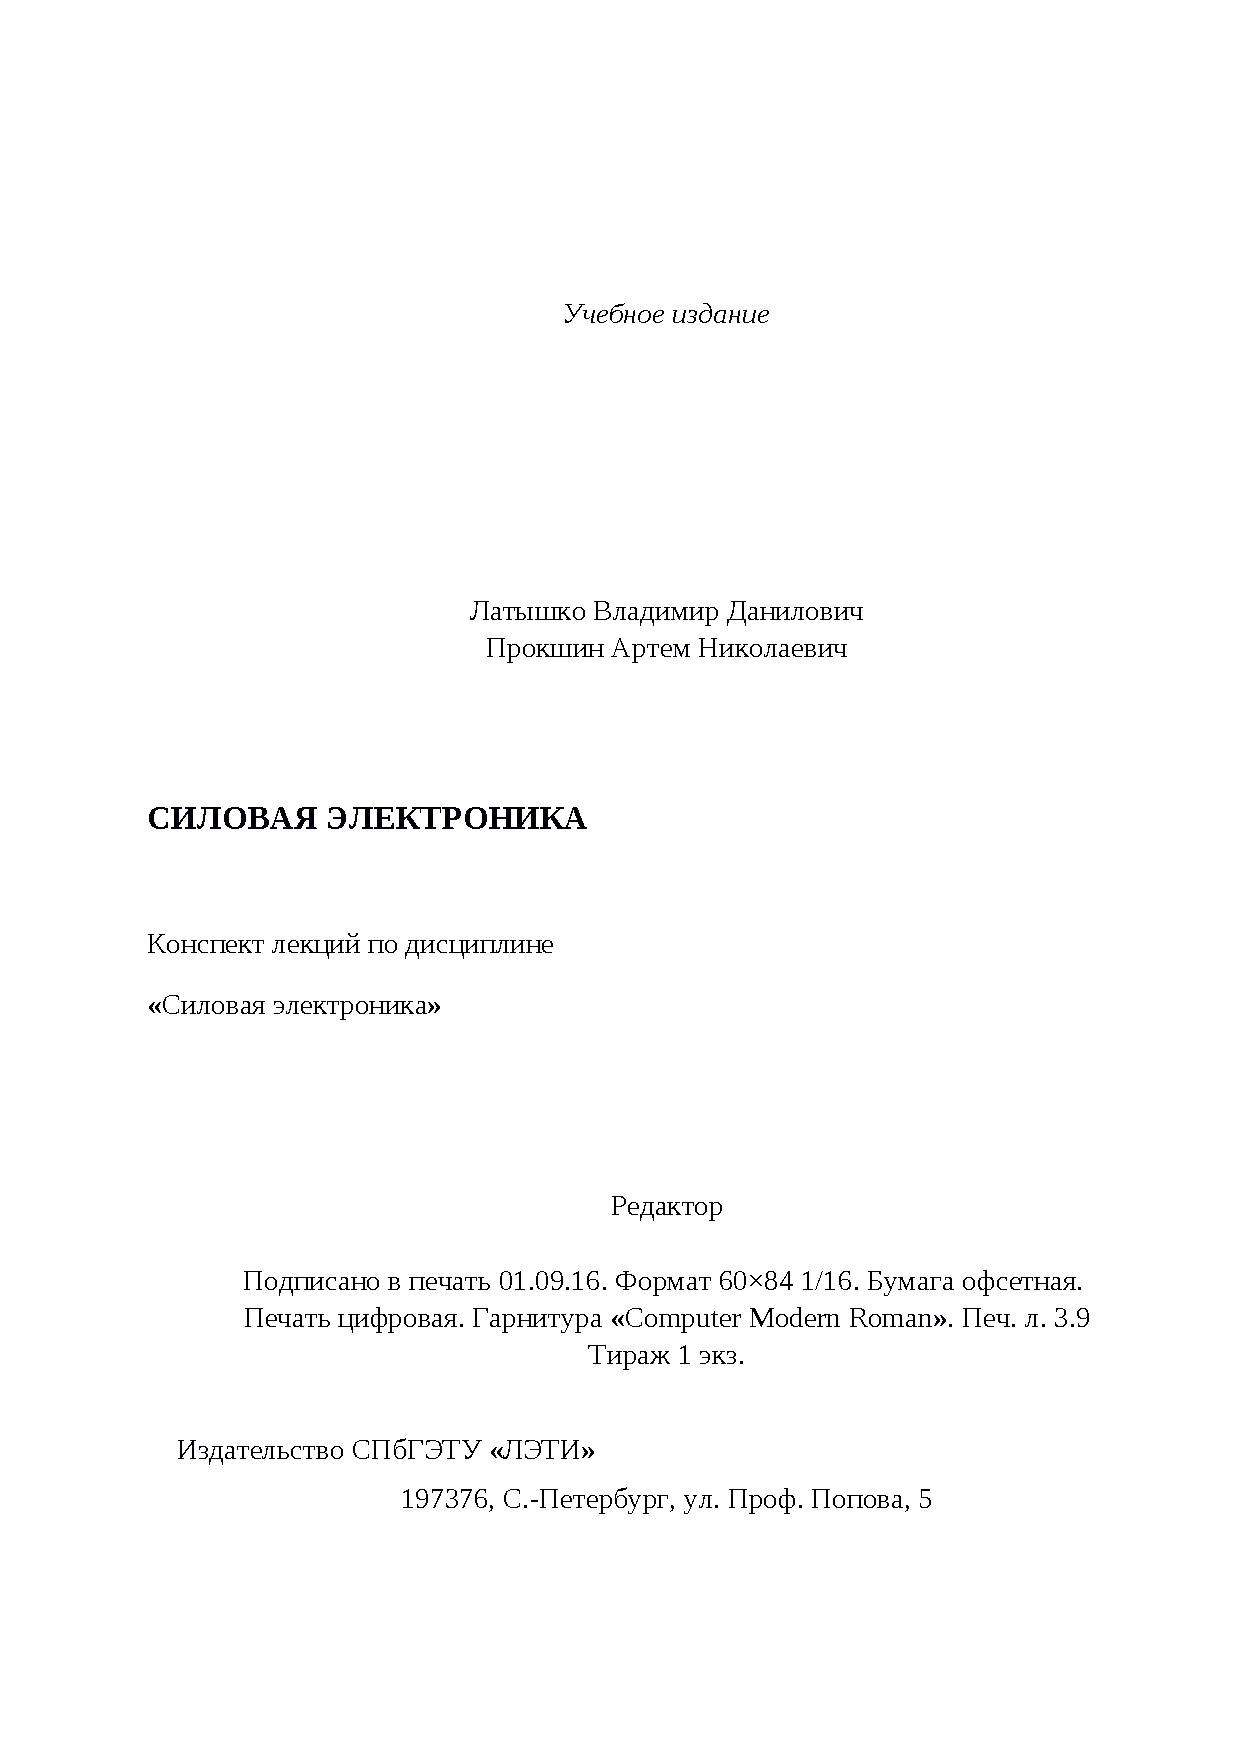
\includepdf[pages=-]{my_22my}
\newpage
\end{document}
